%%
%% This is file `sample-acmsmall.tex',
%% generated with the docstrip utility.
%%
%% The original source files were:
%%
%% samples.dtx  (with options: `acmsmall')
%% 
%% IMPORTANT NOTICE:
%% 
%% For the copyright see the source file.
%% 
%% Any modified versions of this file must be renamed
%% with new filenames distinct from sample-acmsmall.tex.
%% 
%% For distribution of the original source see the terms
%% for copying and modification in the file samples.dtx.
%% 
%% This generated file may be distributed as long as the
%% original source files, as listed above, are part of the
%% same distribution. (The sources need not necessarily be
%% in the same archive or directory.)
%%
%% The first command in your LaTeX source must be the \documentclass command.
%
% \documentclass[acmsmall,screen,nonacm]{acmart}
% \documentclass[acmsmall, authordraft]{acmart}
\documentclass[acmsmall]{acmart}
%
%% NOTE that a single column version is required for 
%% submission and peer review. This can be done by changing
%% the \doucmentclass[...]{acmart} in this template to 
%% \documentclass[manuscript,screen]{acmart}
%% 
%% To ensure 100% compatibility, please check the white list of
%% approved LaTeX packages to be used with the Master Article Template at
%% https://www.acm.org/publications/taps/whitelist-of-latex-packages 
%% before creating your document. The white list page provides 
%% information on how to submit additional LaTeX packages for 
%% review and adoption.
%% Fonts used in the template cannot be substituted; margin 
%% adjustments are not allowed.
%%
\usepackage{colortbl}
\usepackage{arydshln}
\usepackage{multirow}
\usepackage{multicol}
 \usepackage{array}
%% \BibTeX command to typeset BibTeX logo in the docs
\usepackage{bm}
\usepackage{booktabs} % For formal tables
\usepackage{amsmath}
\usepackage{amsfonts}
% \usepackage{amssymb}
\usepackage{graphicx}
\usepackage{tabularx}
\usepackage{textcomp}
\usepackage{xcolor}
\usepackage{listings}
\usepackage{multirow}
\usepackage{subfig}
\usepackage{algorithm}
\usepackage[noend]{algpseudocode}
\usepackage{graphicx}
\usepackage{bbding}



\AtBeginDocument{%
  \providecommand\BibTeX{{%
    \normalfont B\kern-0.5em{\scshape i\kern-0.25em b}\kern-0.8em\TeX}}}

%% Rights management information.  This information is sent to you
%% when you complete the rights form.  These commands have SAMPLE
%% values in them; it is your responsibility as an author to replace
%% the commands and values with those provided to you when you
%% complete the rights form.
\setcopyright{acmcopyright}
\copyrightyear{2021}
\acmYear{2021}
\acmDOI{10.1145/1122445.1122456}


%%
%% These commands are for a JOURNAL article.
\acmJournal{JACM}
\acmVolume{37}
\acmNumber{4}
\acmArticle{111}
\acmMonth{8}

%%
%% Submission ID.
%% Use this when submitting an article to a sponsored event. You'll
%% receive a unique submission ID from the organizers
%% of the event, and this ID should be used as the parameter to this command.
%%\acmSubmissionID{123-A56-BU3}

%%
%% The majority of ACM publications use numbered citations and
%% references.  The command \citestyle{authoryear} switches to the
%% "author year" style.
%%
%% If you are preparing content for an event
%% sponsored by ACM SIGGRAPH, you must use the "author year" style of
%% citations and references.
%% Uncommenting
%% the next command will enable that style.
%%\citestyle{acmauthoryear}

%%
%% end of the preamble, start of the body of the document source.
\begin{document}


\title{Time-aware Path Reasoning on Knowledge Graph for Recommendation}

\newcommand\norm[1]{\left\lVert#1\right\rVert}
\newcommand{\Lapl}{\mathbf{\mathop{\mathcal{L}}}}
\newcommand{\lapl}{\mathcal{L}}
\newcommand{\Trans}[1]{{#1}^{\top}}
\newcommand{\Trace}[1]{tr\left({#1}\right)}
\newcommand{\Bracs}[1]{\left({#1}\right)}
\newcommand{\Mat}[1]{\textbf{#1}}
\newcommand{\MatS}[3]{\mathbf{#1}^{#2}_{#3}}
\newcommand{\Space}[1]{\mathbb{#1}}
\newcommand{\Set}[1]{\mathcal{#1}}
\newcommand{\vectornorm}[1]{\left|\left|#1\right|\right|}
\newcommand{\bpi}{\boldsymbol{\pi}}
\newcommand{\BlockMat}[2]{\left[\begin{matrix}#1\\#2\end{matrix}\right]}
\newcommand{\BlockMatSquare}[4]{\left[\begin{matrix}#1 & #2\\#3 & #4\end{matrix}\right]}
% \newcommand{\ParaTitle}[1]{\vspace{5pt}\noindent\textbf{#1}}
\newcommand{\ParaTitle}[1]{\noindent\textbf{#1}}
\newcommand\at[2]{\left.#1\right|_{#2}}

\newcommand{\ie}{{\em i.e.}}
\newcommand{\eg}{{\em e.g.}}
\newcommand{\etal}{{\em et al.}}
\newcommand{\etc}{{\em etc.}}
\newcommand{\tkgrec}{TPRec}


%%
%% The "title" command has an optional parameter,
%% allowing the author to define a "short title" to be used in page headers.


%%
%% The "author" command and its associated commands are used to define
%% the authors and their affiliations.
%% Of note is the shared affiliation of the first two authors, and the
%% "authornote" and "authornotemark" commands
%% used to denote shared contribution to the research.

\author{Yuyue Zhao}
\email{yyzha0@mail.ustc.edu.cn}
\affiliation{%
  \institution{University of Science and Technology of China}
%   \institution{Key Laboratory of Cyberculture Content Cognition and Detection, Ministry of Culture and Tourism} 
  \country{China}
  }


\author{Xiang Wang}
\authornote{Corresponding Author.}
\email{xiangwang1223@gmail.com}
\affiliation{%
  \institution{University of Science and Technology of China}
%   \institution{Key Laboratory of Cyberculture Content Cognition and Detection, Ministry of Culture and Tourism} 
  \country{China}
  }
  
\author{Jiawei Chen}
\email{cjwustc@ustc.edu.cn}
\affiliation{%
  \institution{University of Science and Technology of China}
%   \institution{Key Laboratory of Cyberculture Content Cognition and Detection, Ministry of Culture and Tourism} 
  \country{China}
  }
  
  \author{Yashen Wang}
\email{yswang@bit.edu.cn}
\affiliation{%
  \institution{National Engineering Laboratory 
        for Risk Perception and Prevention (RPP)}
  \country{China}
  }

 \author{Wei Tang}
\email{weitang@mail.ustc.edu.cn}
\affiliation{%
  \institution{University of Science and Technology of China}
%   \institution{Key Laboratory of Cyberculture Content Cognition and Detection, Ministry of Culture and Tourism} 
  \country{China}
  }


\author{Xiangnan He}
\email{xiangnanhe@gmail.com}
\affiliation{%
  \institution{University of Science and Technology of China}
  \streetaddress{96 JinZhai Road}
  \city{Hefei}
  \country{China}
}


\author{Haiyong Xie}
\authornote{Corresponding Author.}
\email{haiyong.xie@ieee.org}
\affiliation{
%  \institution{University of Science and Technology of China}
  \institution{Key Laboratory of Cyberculture Content Cognition and Detection, Ministry of Culture and Tourism, }
  \institution{Advanced Innovation Center for Human Brain Protection, Capital Medical University}
  \country{China}
  \streetaddress{The authors from the University of Science and Technology of China are affliated with the CCCD Key Lab of MCT}
  }


% \author{Ben Trovato}
% \authornote{Both authors contributed equally to this research.}
% \email{trovato@corporation.com}
% \orcid{1234-5678-9012}
% \author{G.K.M. Tobin}
% \authornotemark[1]
% \email{webmaster@marysville-ohio.com}
% \affiliation{%
%   \institution{Institute for Clarity in Documentation}
%   \streetaddress{P.O. Box 1212}
%   \city{Dublin}
%   \state{Ohio}
%   \country{USA}
%   \postcode{43017-6221}
% }

% \author{Lars Th{\o}rv{\"a}ld}
% \affiliation{%
%   \institution{The Th{\o}rv{\"a}ld Group}
%   \streetaddress{1 Th{\o}rv{\"a}ld Circle}
%   \city{Hekla}
%   \country{Iceland}}
% \email{larst@affiliation.org}

% \author{Valerie B\'eranger}
% \affiliation{%
%   \institution{Inria Paris-Rocquencourt}
%   \city{Rocquencourt}
%   \country{France}
% }

% \author{Aparna Patel}
% \affiliation{%
%  \institution{Rajiv Gandhi University}
%  \streetaddress{Rono-Hills}
%  \city{Doimukh}
%  \state{Arunachal Pradesh}
%  \country{India}}

% \author{Huifen Chan}
% \affiliation{%
%   \institution{Tsinghua University}
%   \streetaddress{30 Shuangqing Rd}
%   \city{Haidian Qu}
%   \state{Beijing Shi}
%   \country{China}}

% \author{Charles Palmer}
% \affiliation{%
%   \institution{Palmer Research Laboratories}
%   \streetaddress{8600 Datapoint Drive}
%   \city{San Antonio}
%   \state{Texas}
%   \country{USA}
%   \postcode{78229}}
% \email{cpalmer@prl.com}

% \author{John Smith}
% \affiliation{%
%   \institution{The Th{\o}rv{\"a}ld Group}
%   \streetaddress{1 Th{\o}rv{\"a}ld Circle}
%   \city{Hekla}
%   \country{Iceland}}
% \email{jsmith@affiliation.org}

% \author{Julius P. Kumquat}
% \affiliation{%
%   \institution{The Kumquat Consortium}
%   \city{New York}
%   \country{USA}}
% \email{jpkumquat@consortium.net}

%%
%% By default, the full list of authors will be used in the page
%% headers. Often, this list is too long, and will overlap
%% other information printed in the page headers. This command allows
%% the author to define a more concise list
%% of authors' names for this purpose.
\renewcommand{\shortauthors}{Zhao, et al.}

%%
%% The abstract is a short summary of the work to be presented in the
%% article.

\begin{abstract}
%Knowledge graphs have been widely used in recommendation systems due to their 
% structured auxiliary data as well as potential support for reasoning. 
% In 
% particular, multi-hop connections on knowledge graphs can provide 
% explicit reasoning paths reflecting the working mechanism. 
% However, the temporal
% user-item interaction data can be used to facilitate reasoning but is usually 
% overlooked in existing studies. In this paper, we propose a novel method, 
% referred to as Temporal Knowledge Graph reasoning for Recommendation (TKGRec),
%% \footnote{github} 
% to better enhance explainable recommendation 
% by leveraging temporal information. Specifically, we propose a time-series 
% clustering technique to construct temporal knowledge graphs (TKGs), and then 
% encode the TKG for proper semantic representation. Furthermore, we propose a 
% time-aware path reasoning method for recommendation. Experiments on three 
% real-world datasets show that our method TGRec achieves substantial gains and 
% can successfully employ TKGs to improve the quality of explainable 
% recommendation.


Reasoning on knowledge graph (KG) has been studied for explainable recommendation due to its ability of providing explicit explanations.
    However, current KG-based explainable recommendation methods unfortunately
    ignore the temporal information (such as purchase time,
    recommend time, \etc), which may result in unsuitable explanations.
    % To improve the predictive capacity, we adopt temporal information with 
    % path reasoning for developing effective recommendation.
    % However, timestamps in recommender systems are likely to be numerous, 
    % ambiguous and from distinct sources. 
    % %
    % It is not easy to directly apply temporal information to promote path
    % reasoning over KGs.
%
In this work, we propose a novel  {\it Time-aware Path reasoning 
for Recommendation} (\tkgrec\ for short) method, which leverages the potential 
of temporal information to offer better recommendation with plausible
    explanations.
%
First, we present an efficient time-aware interaction relation 
extraction component
    to construct collaborative knowledge graph with time-aware interactions 
    (TCKG for short), and then 
    introduce
    a novel time-aware path reasoning  method for recommendation.  We conduct
    extensive experiments on three real-world datasets. The results demonstrate that the proposed \tkgrec\ could successfully
    employ TCKG to achieve substantial gains and improve the quality of 
    explainable recommendation. 

\end{abstract}

% \footnote{The authors from the University of Science and Technology of China are affliated with the CCCD Key Lab of MCT.}


%%
%% The code below is generated by the tool at http://dl.acm.org/ccs.cfm.
%% Please copy and paste the code instead of the example below.
%%
\begin{CCSXML}
<ccs2012>
<concept>
<concept_id>10002951.10003317.10003347.10003350</concept_id>
<concept_desc>Information systems~Recommender systems</concept_desc>
<concept_significance>500</concept_significance>
</concept>
</ccs2012>
\end{CCSXML}

\ccsdesc[500]{Information systems~Recommender systems}

\keywords{Explainable Recommendation; Temporal Knowledge Graphs; Reinforcement Learning;}

\maketitle


\section{Introduction}

% 1. 引出KG reasoning

Recently, knowledge graphs (KGs) have been widely used in 
recommender systems
due to their rich structured knowledge
%(i.e., entities' background knowledge and relations amongst entities) 
 (\eg, \cite{ripplenet, pgpr, CKE, DKN, KSR, shine, 
ADAC, wu2021disenkgat, zeng2022shadewatcher,
RNNexpl}). A KG is a type of directed heterogeneous graph in which nodes 
represent
real-world \textit{entities} and edges represent their \textit{relations}.
%in which nodes correspond to \textit{entities} and edges correspond to
%\textit{relations}.
%
Reasoning over KGs \cite{pgpr, ADAC} for recommendation can not 
only infer user preferences more accurately, but also
offer each recommended item with a multi-hop path. Such 
knowledge-aware paths allow us to explain why an item is recommended, so as to increase users' satisfaction and trust \cite{surveyExp, 
effectiveRec}.
%
% Using reinforcement learning agents promises to automatically mine and reason
% over such paths.
Existing methods adopt reinforcement learning agents to automatically mine and reason over such paths.
The core lies in  using 
% $\bm{(User, {Purchase}, [?])}$
\textbf{"What items will users purchase?"}
 to guide the 
reasoning process towards the target items.

% ============================================================================

% \begin{figure*}[tb]
% %\setlength{\abovecaptionskip}{0.cm}
% %\setlength{\belowcaptionskip}{-0.cm}
%     \begin{minipage}[b]{0.415\textwidth}
%         \centering
%         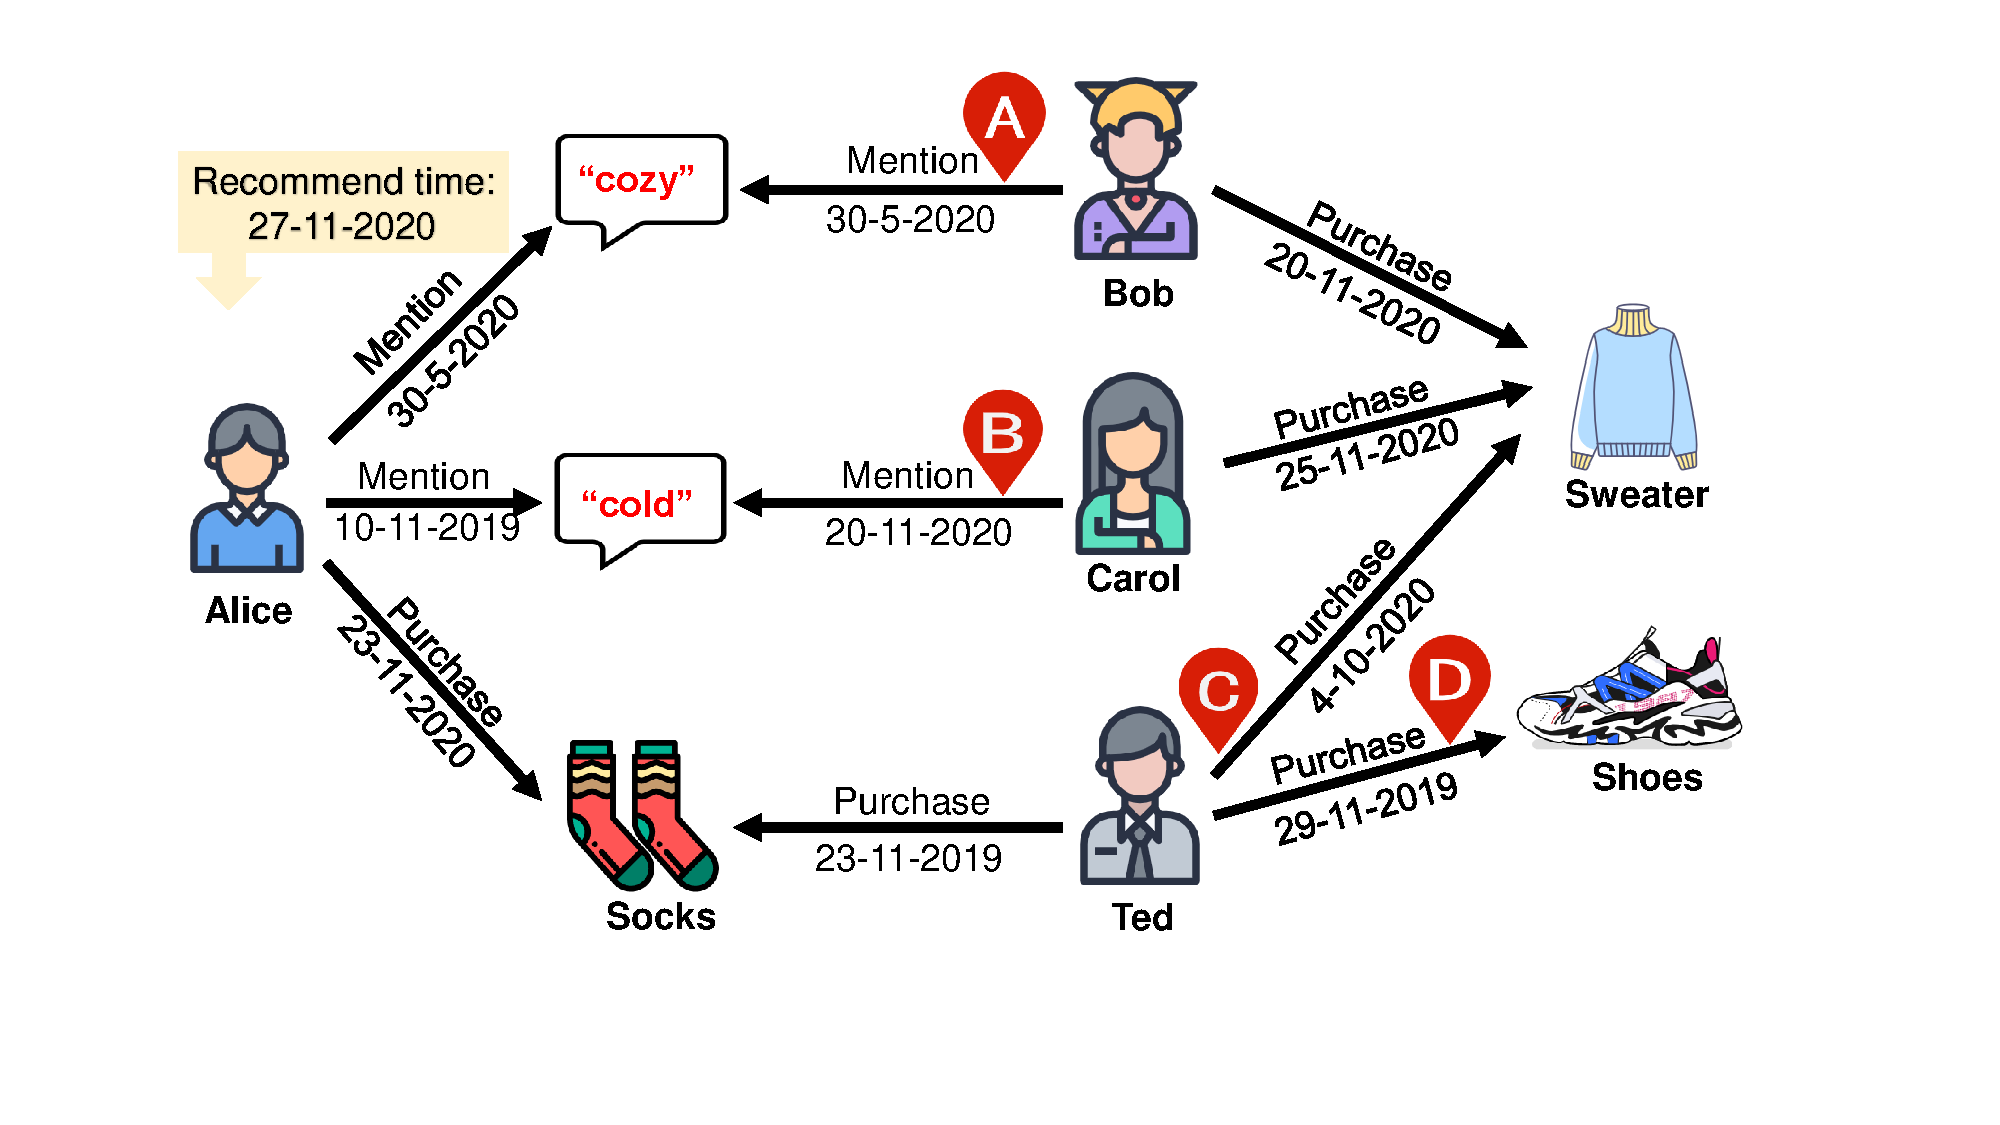
\includegraphics[width=0.99\textwidth]{chart/intro_emp.pdf}
% 		\caption{Example of how temporal information assists in explainable 
%         recommendation.}
%         \label{intro_exp}
%     \end{minipage}
%     \hfill
%     \begin{minipage}[b]{0.575\textwidth}
%         \centering
%         \subfloat[Clothing]{
%             \centering
%             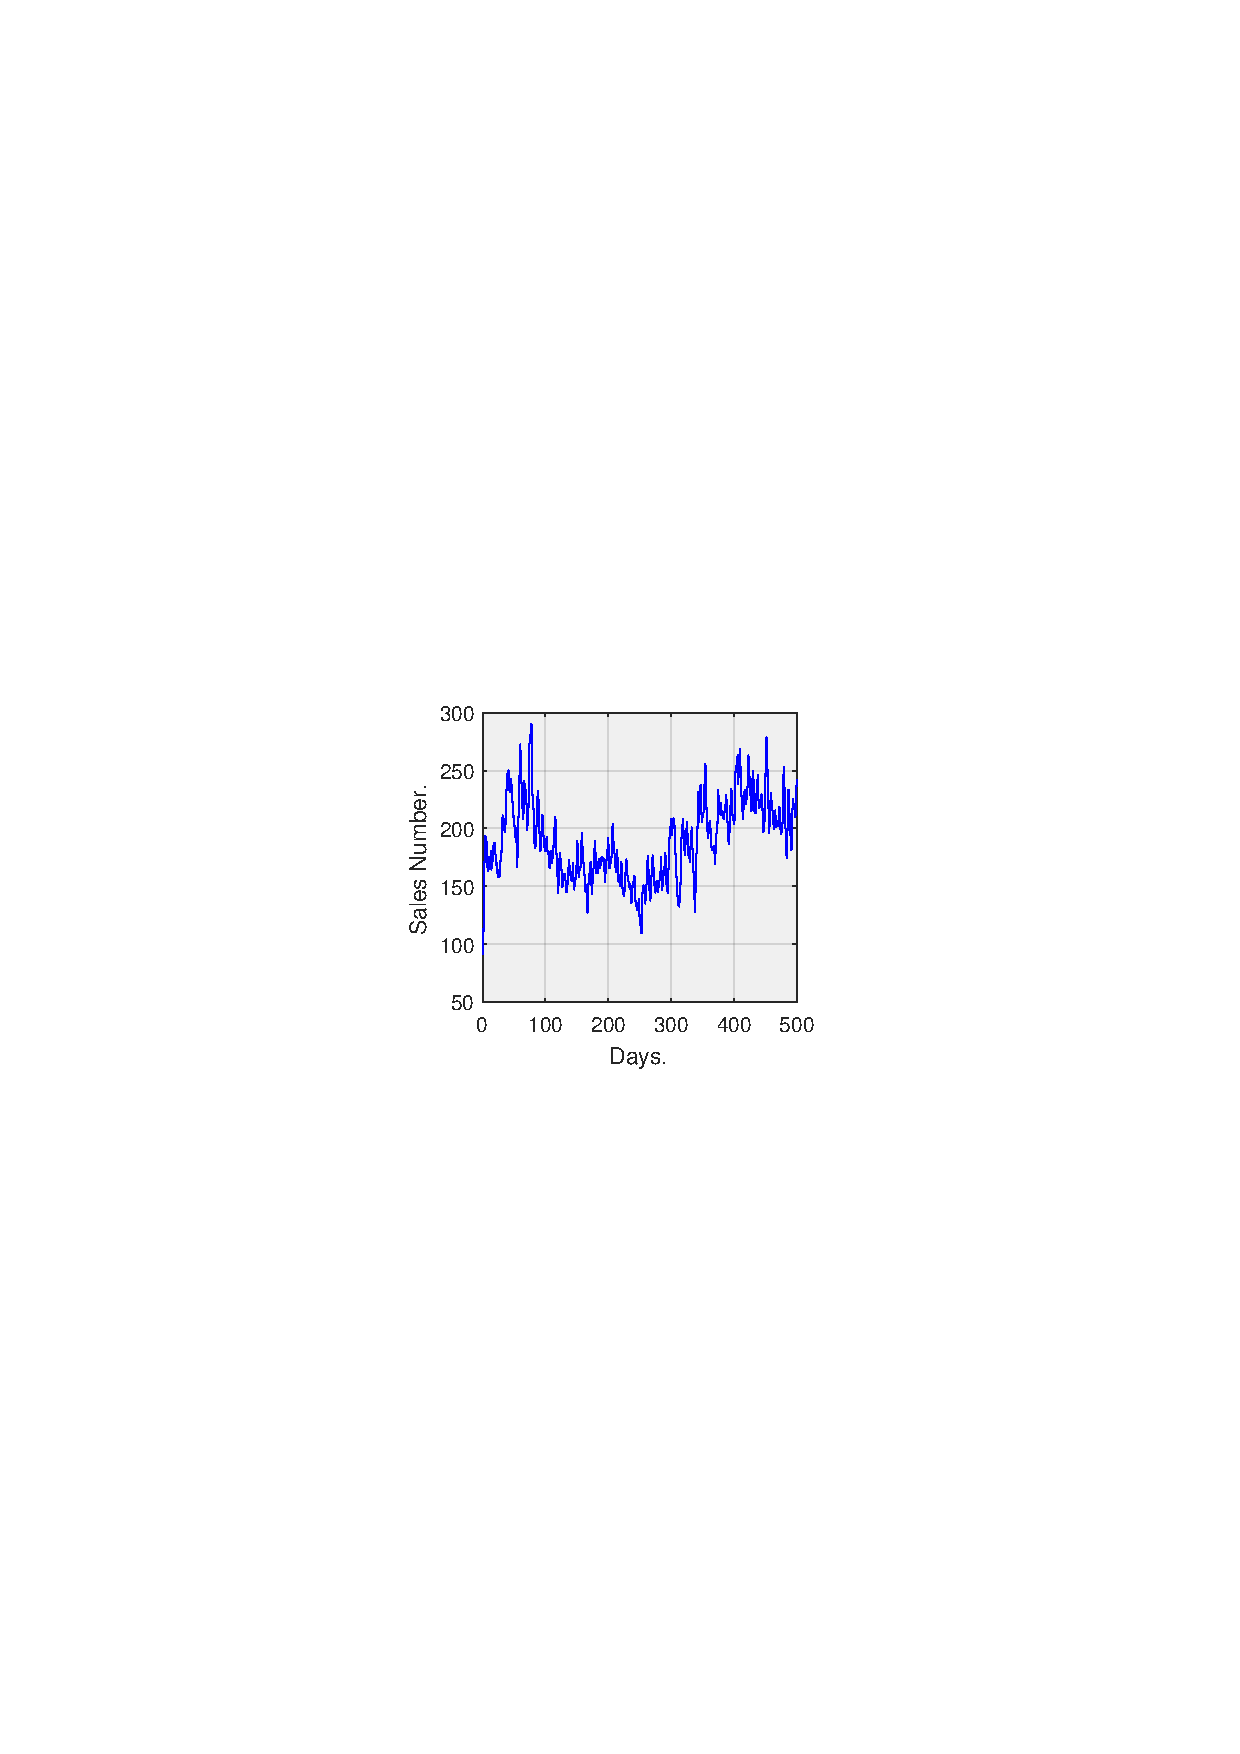
\includegraphics[width=0.345\textwidth]{chart/day_beauty.pdf}
%             \label{day_Cloth}
%         }
%         %
%         \subfloat[Cell Phones.]{
%             \centering
%             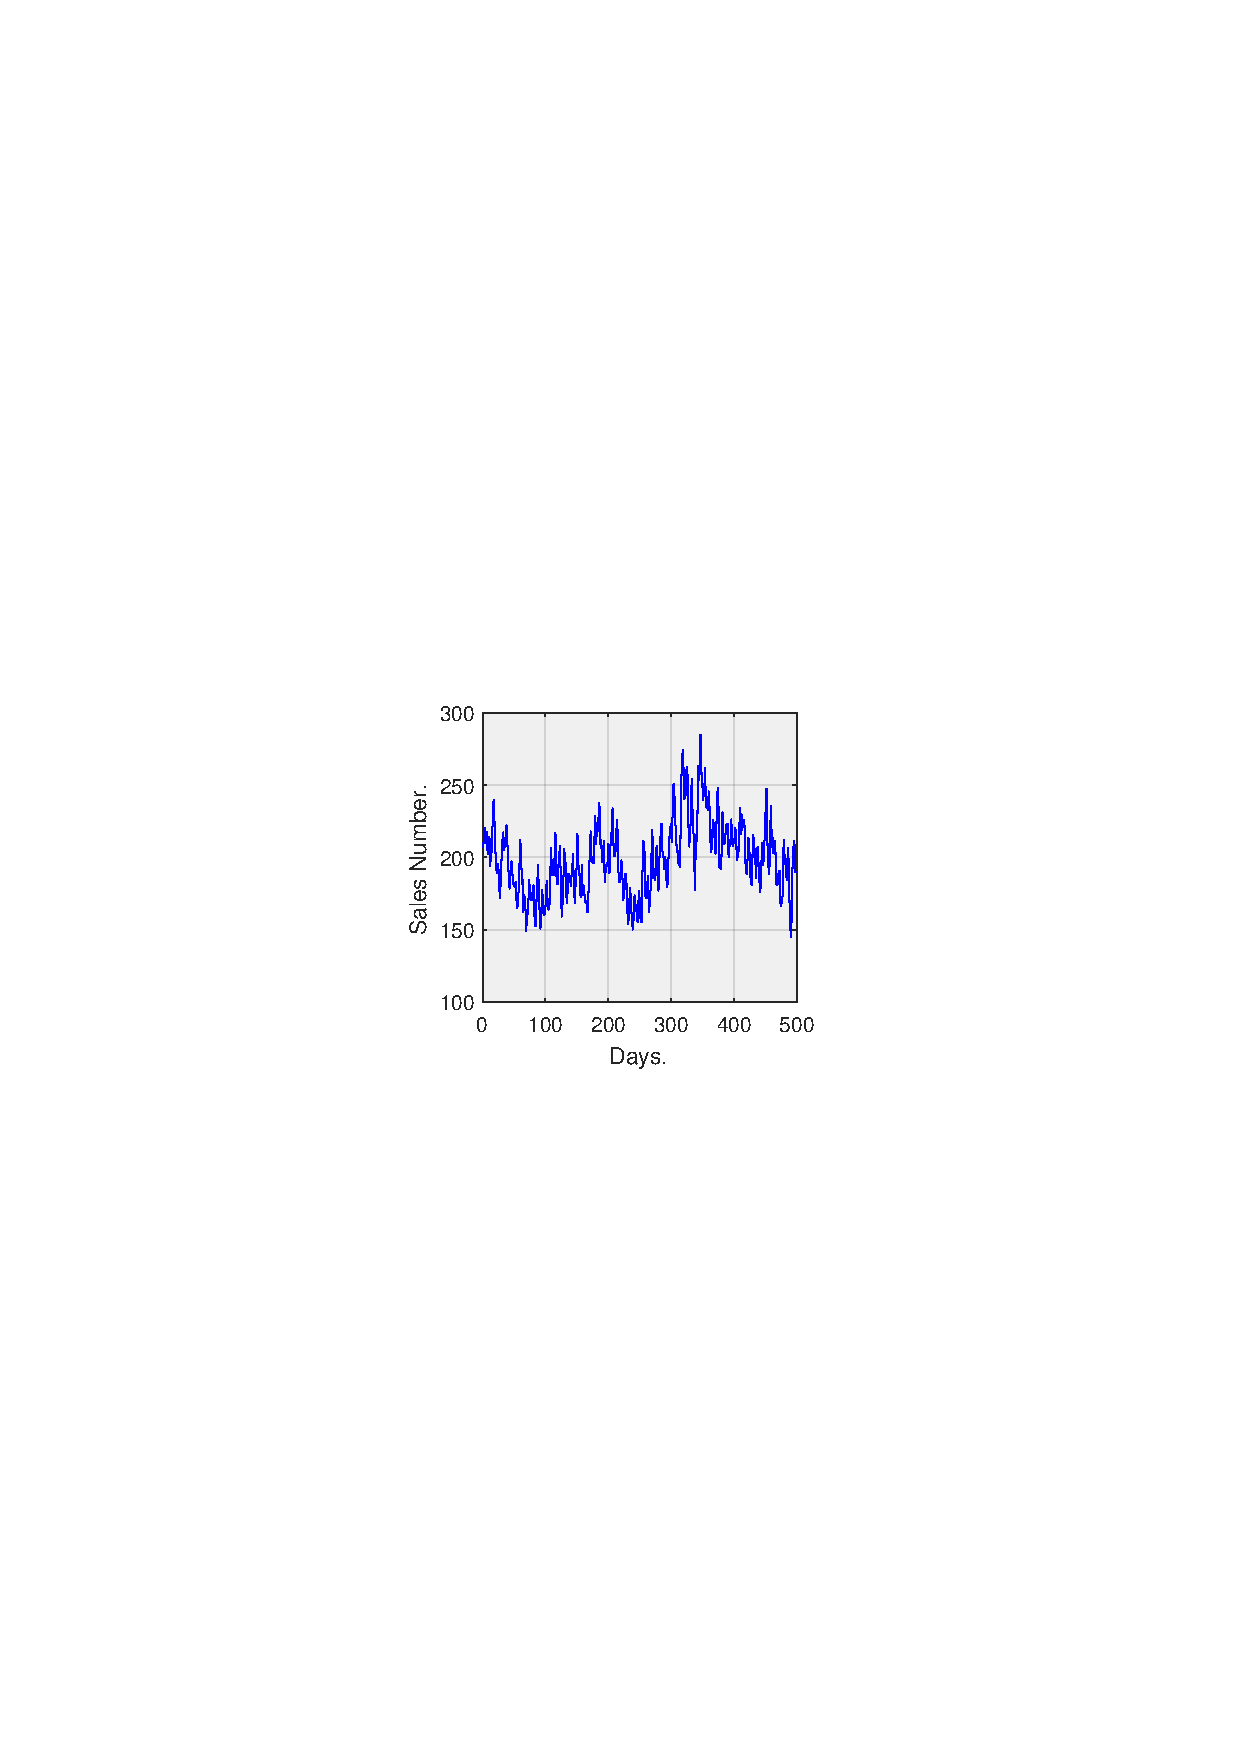
\includegraphics[width=0.345\textwidth]{chart/day_cell.pdf}
%             \label{day_Cell}
%         }
%         %
%         \subfloat[Beauty]{
%             \centering
%             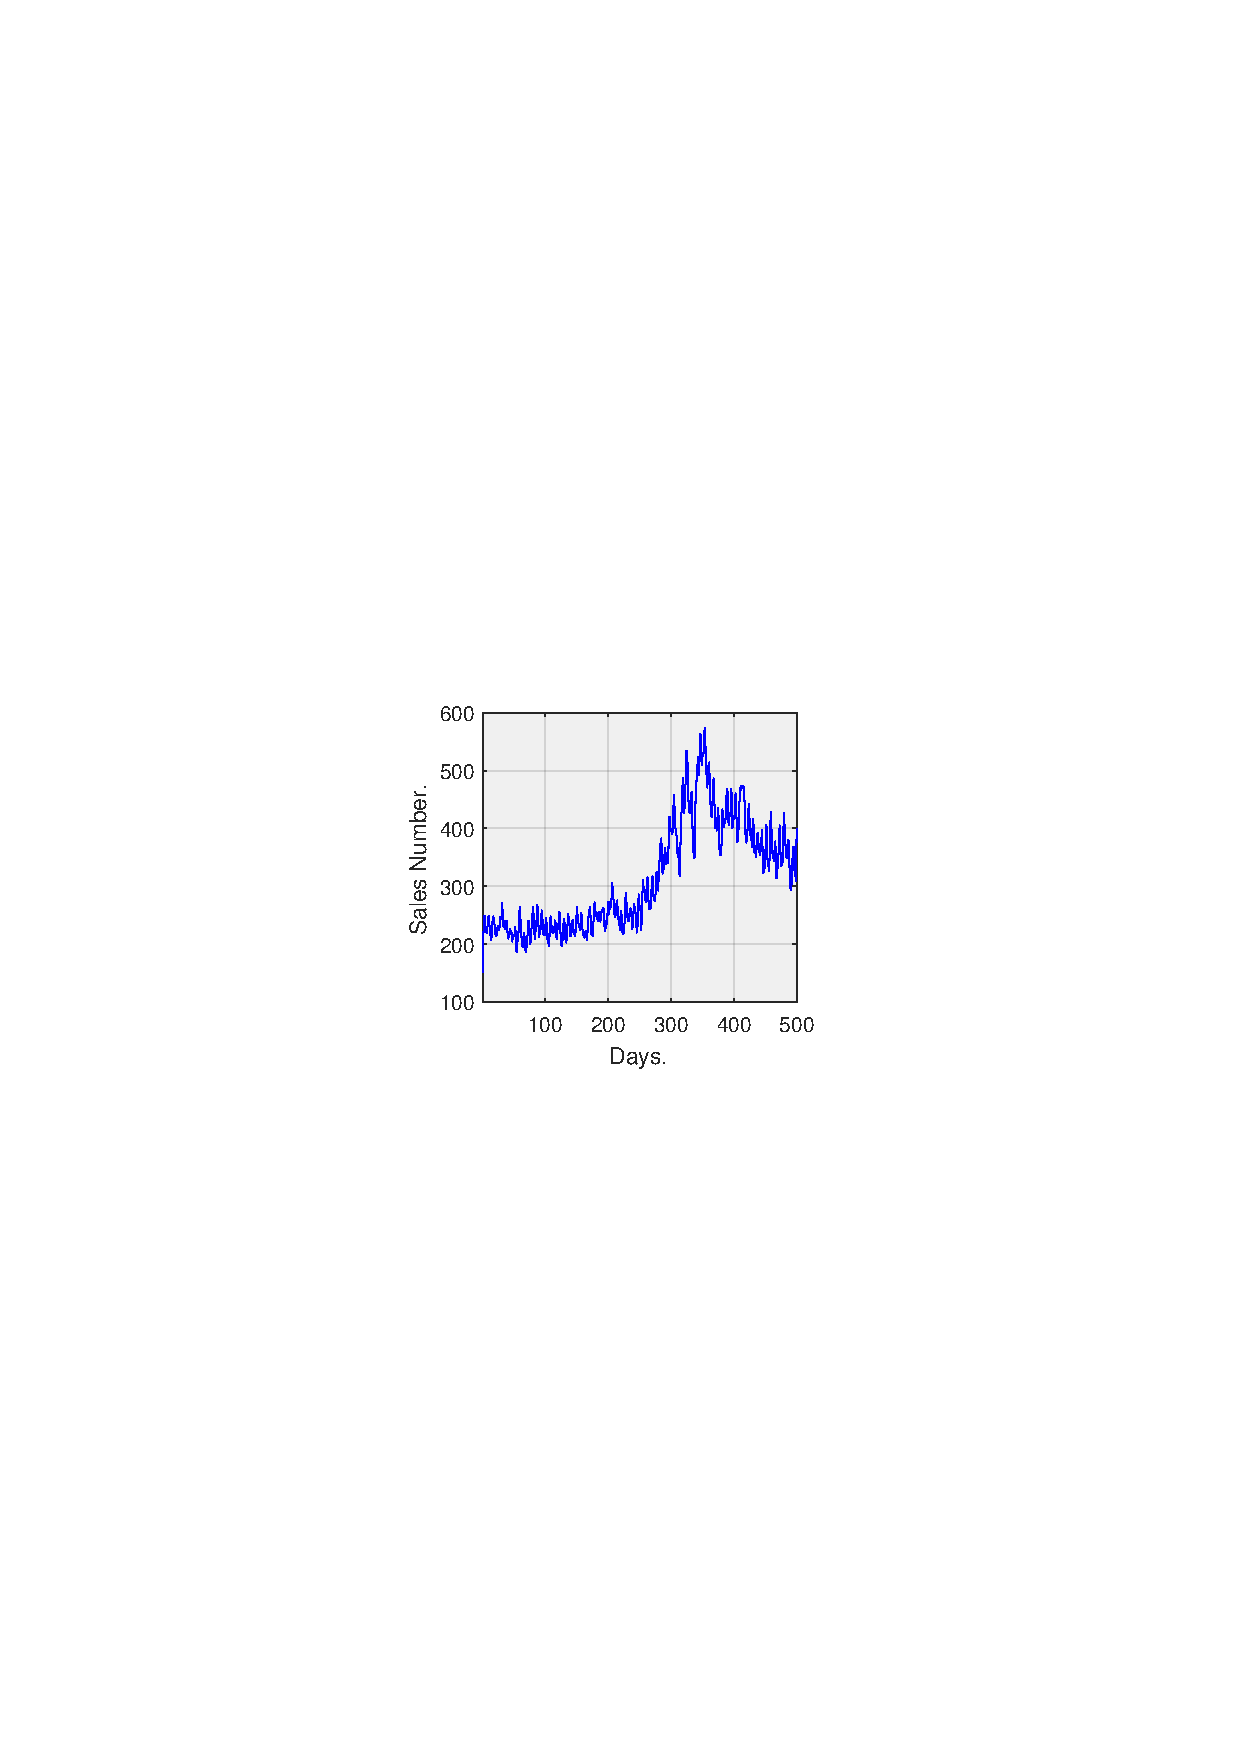
\includegraphics[width=0.345\textwidth]{chart/day_cloth.pdf}
%             \label{day_Beauty}
%         }
%         %
%         \caption{Sales behavior in three Amazon datasets.} 
%         \label{day_cmp}
%     \end{minipage}
% %    \setlength{\abovecaptionskip}{-1pt}
%     \vspace{-0.15cm}
% \end{figure*}

\begin{figure}[!t]
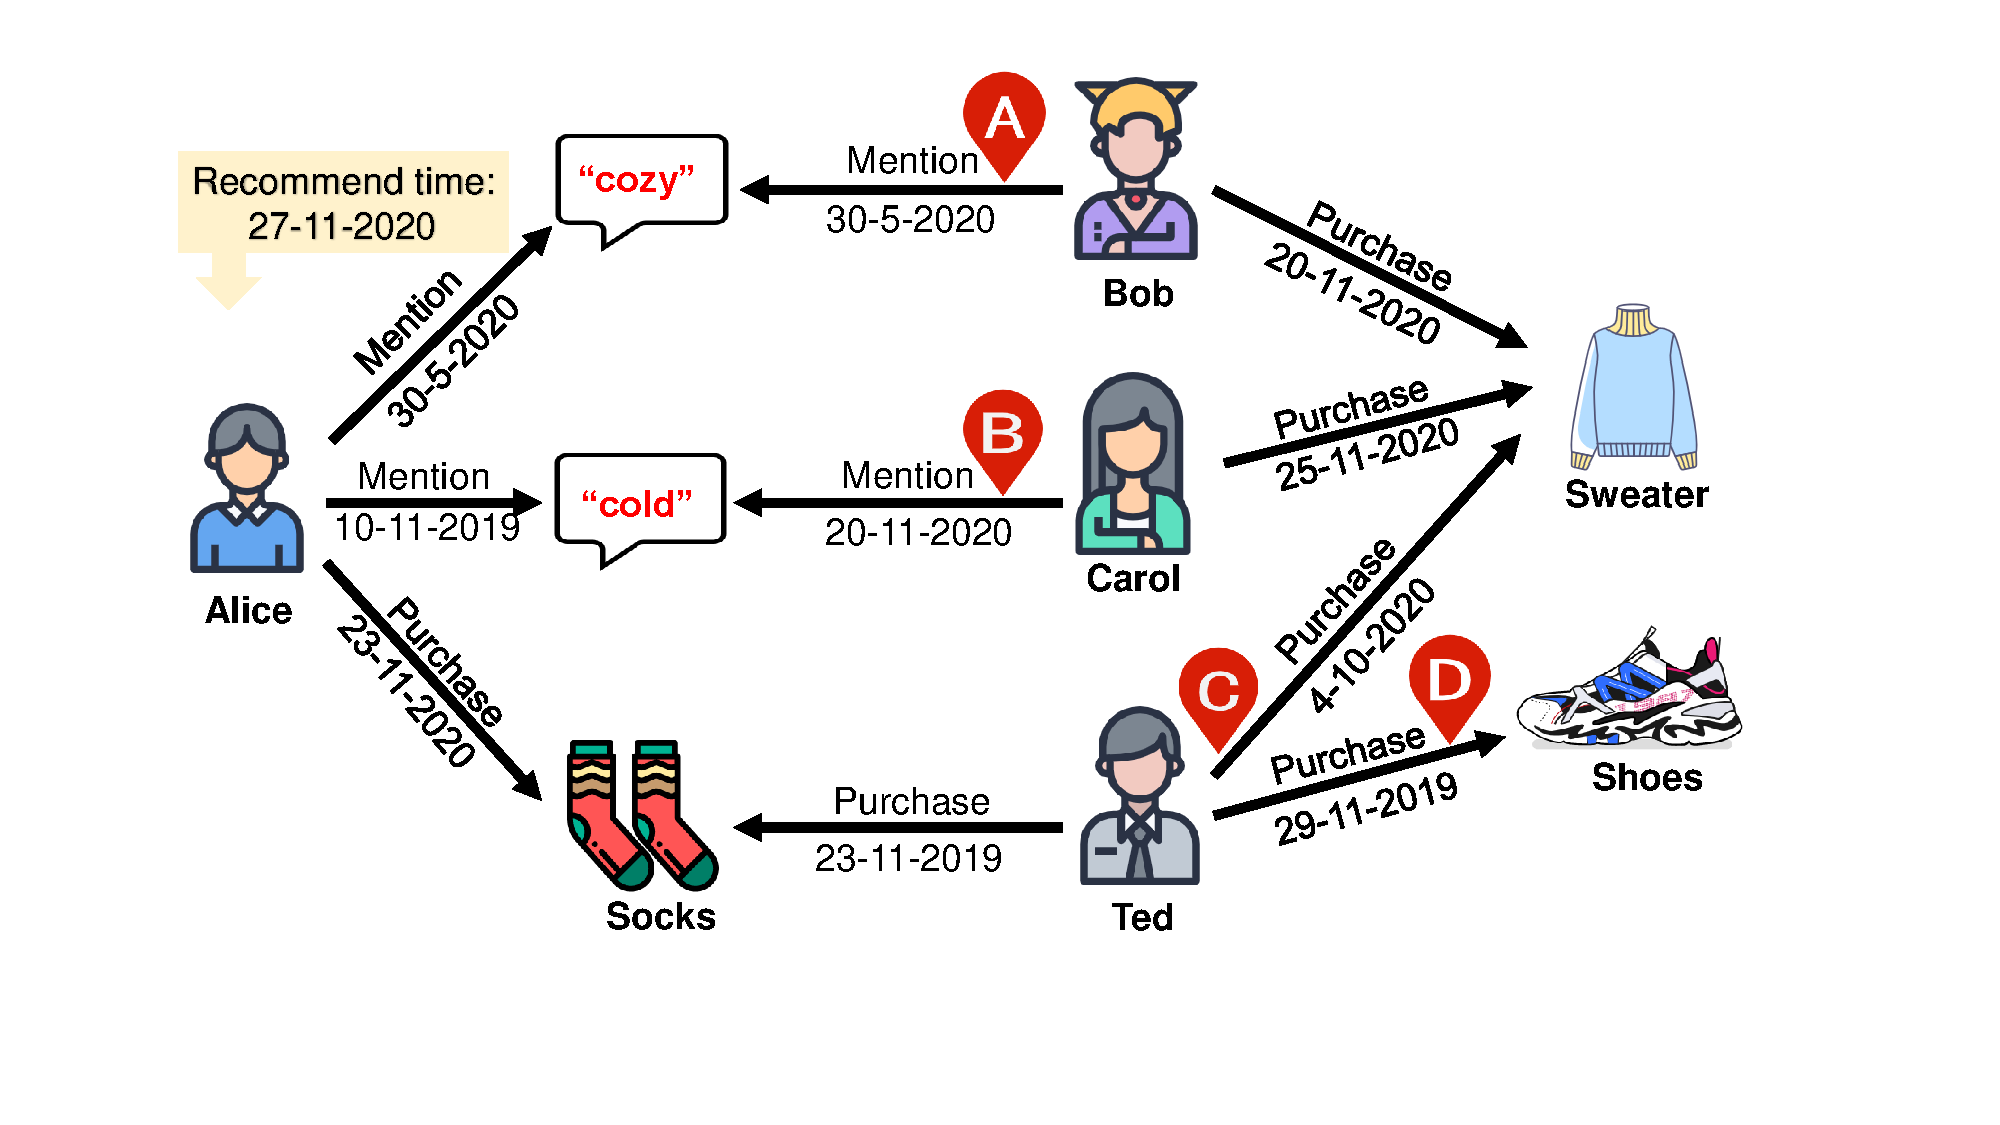
\includegraphics[width=0.7\columnwidth]{chart/intro_emp.pdf}
\caption{Example of how temporal information assists in explainable 
        recommendation.}
\label{intro_exp}
\end{figure}





% ============================================================================

However, current RL agents mostly treat the user-item interaction as the static 
relation, and ignore the time-aware information of interactions (\eg, purchase 
time).
Hence, they fall short in modeling the temporal patterns of user behaviors, 
possibly offering unreliable reasoning paths and recommendations.
%
Considering the example in Figure
\ref{intro_exp}, where A, B, C and D marked in red indicate different reasoning
paths. 
%
Typical KG reasoning methods (\eg, \cite{pgpr, ADAC}) may recommend
$Sweater$ to $Alice$, which can be explained by the path A existing in the
corresponding KG, namely, $Alice \stackrel{Mention}{\longrightarrow}\text{cozy}
\stackrel{Mentioned\_by}{\longrightarrow}Bob
\stackrel{Purchase}{\longrightarrow}Sweater$. 
%
However, with the help of temporal information, it can be shown that
the reasoning paths B and D are better than  A and C. 
%
First, in explaining the same recommendation $Sweater$, path B is more reasonable than A since its relation time (10-11-2019) is
in the season of winter, which is consistent with the recommendation time
(27-11-2020).  This implies the periodic patterns of user behaviors. 
%
Second, path D is better than C since the purchase time 29-11-2019 and
recommendation time 27-11-2020 are both Black Friday while 4-10-2020 is closer to 27-11-2020 only in linear time.
People tend to have similar behaviors in shopping festivals.
% Notably, another example is shown where \underline{Path C} and \underline{Path
% D} meet the branch at $Ted$. 
% Obviously the purchase time 4-10-2020 is closer to
% 27-11-2020 in linear time compared with 29-11-2019, while 29-11-2019 and
% 27-11-2020 are both Black Friday and people tend to have similar behaviors in
% shopping festivals. 
In this sense, we consider Path D a better recommendation.
%
Therefore, a time-aware KG reasoning method is more 
likely to generate better recommendation results.
%, thus makes \underline{Path D} $Shoes$ a better recommendation.

% 3.1 关键的第三段：突然冒出的两个challenge太突兀了。review并不清楚什么是 
%temporal
%knowledge graph(TKG)，他的意义在哪。还有写自己解决的问题的motivation的时候，
%不要用Inspired by。。。
%这个一般是讲方法的时候，我们利用XX方法来解决问题，会用inspired by。
%
%第三段需要捋一下：
%首先总结：考虑时间信息很重要但很有挑战，时间信息很难去建模，时间上的相近并不意
%味着有相似的行为。简单的作为特征的话自然不work。这里可以多讨论一下难点。因此，
%需
%要专门去建模他，以提升效果。 
%时间建模的难点: 1. 怎么合适建模? 难点是啥.
%2. 怎么TKG建模? 难点是啥.
%According to those observations,
\begin{figure}[!t]
    \begin{minipage}[b]{\columnwidth}
        \centering
        \subfloat[Clothing]{
            \centering
            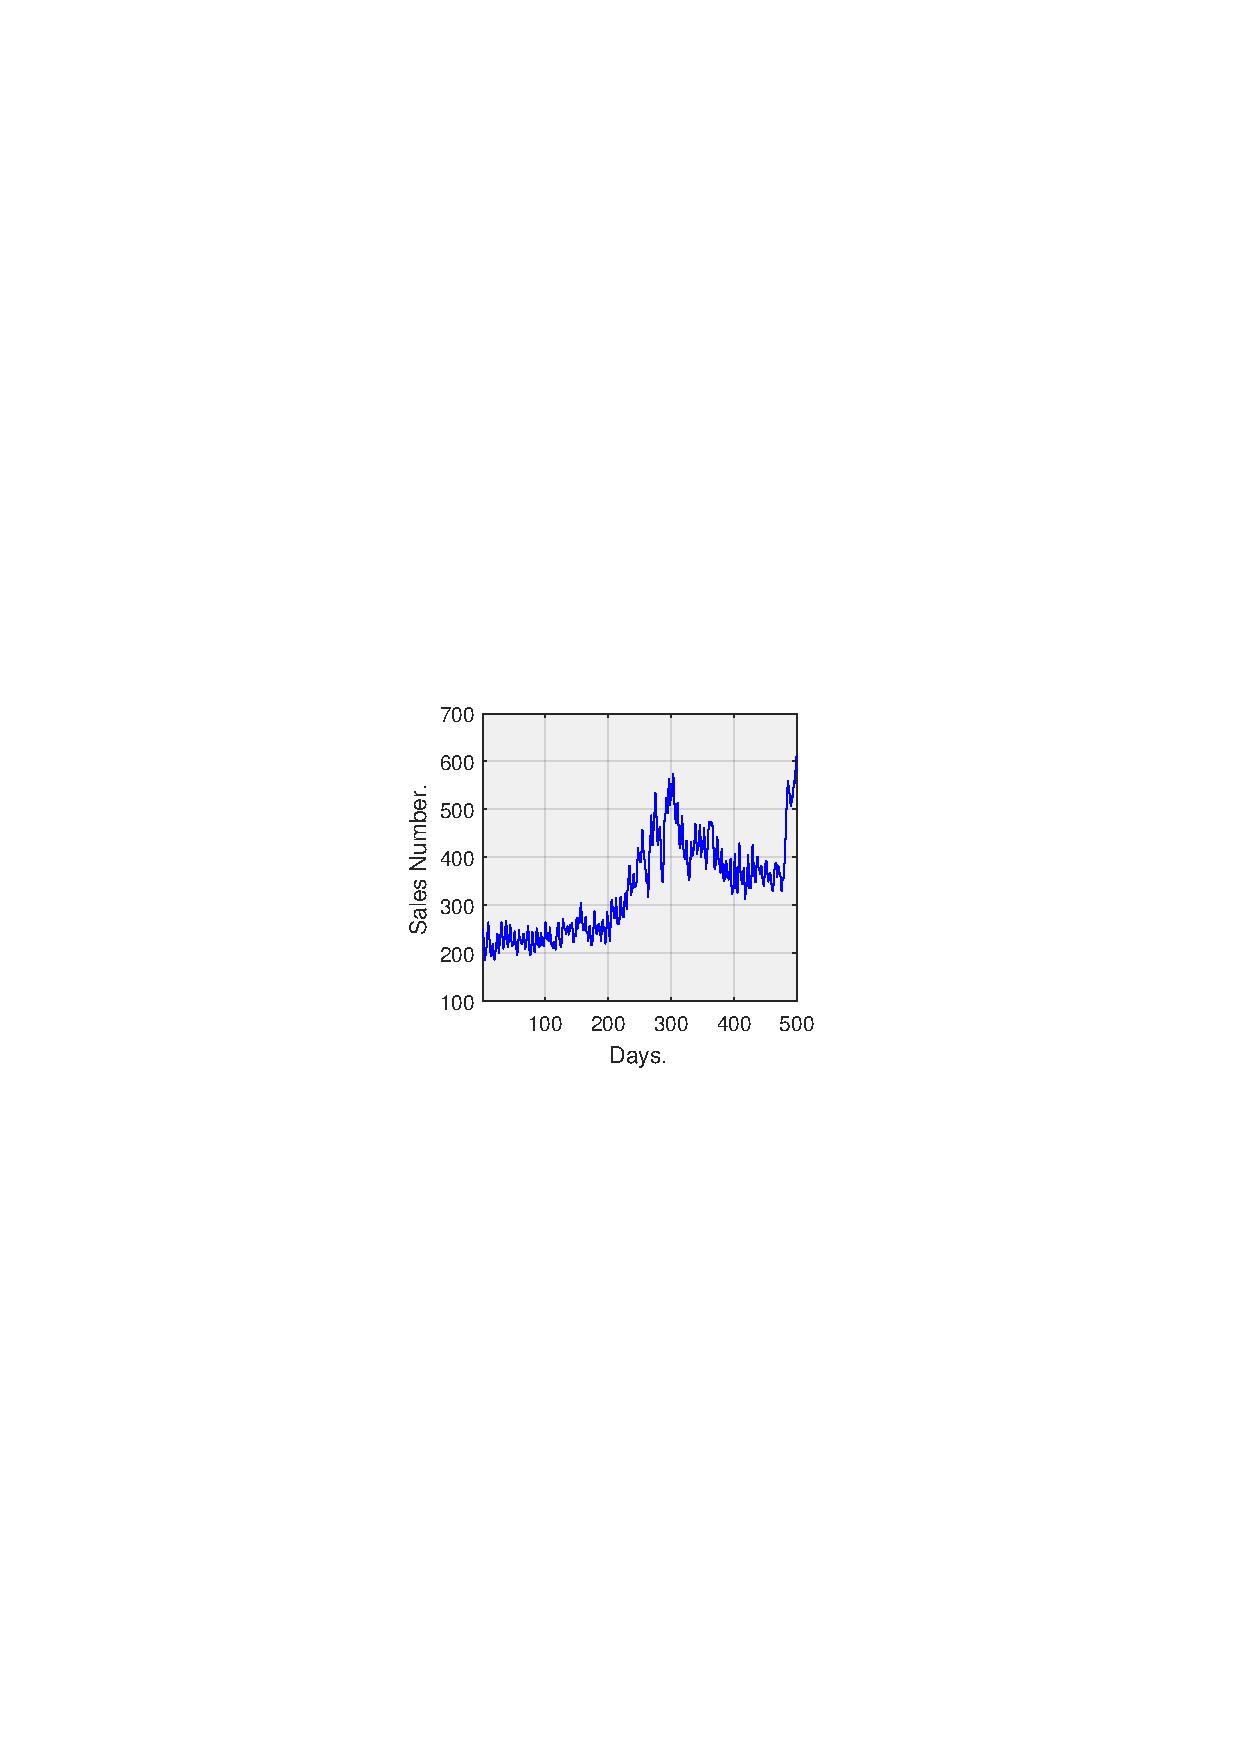
\includegraphics[width=0.33\columnwidth]{chart/day_clo2.pdf}
            \label{day_Cloth}
        }
        %
        \subfloat[Cell Phones.]{
            \centering
            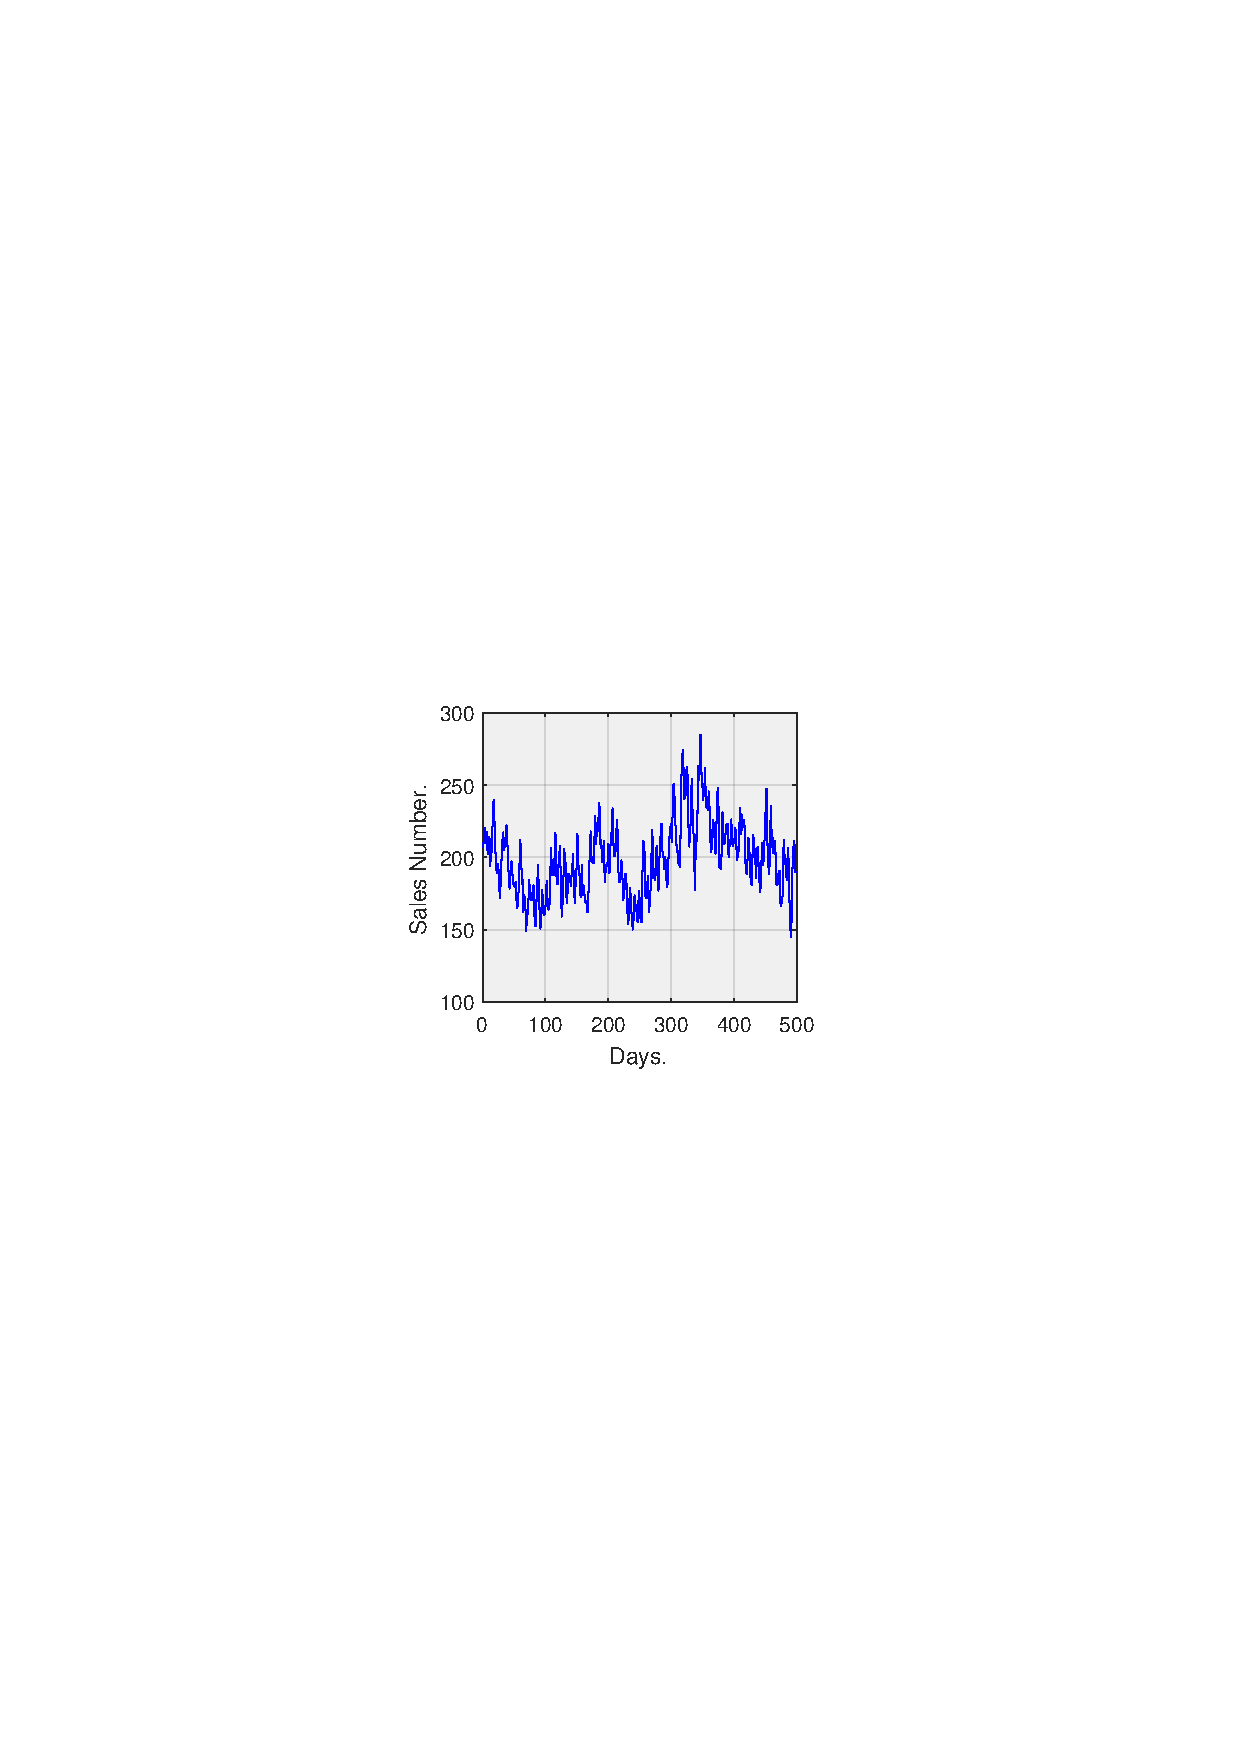
\includegraphics[width=0.33\columnwidth]{chart/day_cell.pdf}
            \label{day_Cell}
        }
        %
        \subfloat[Beauty]{
            \centering
            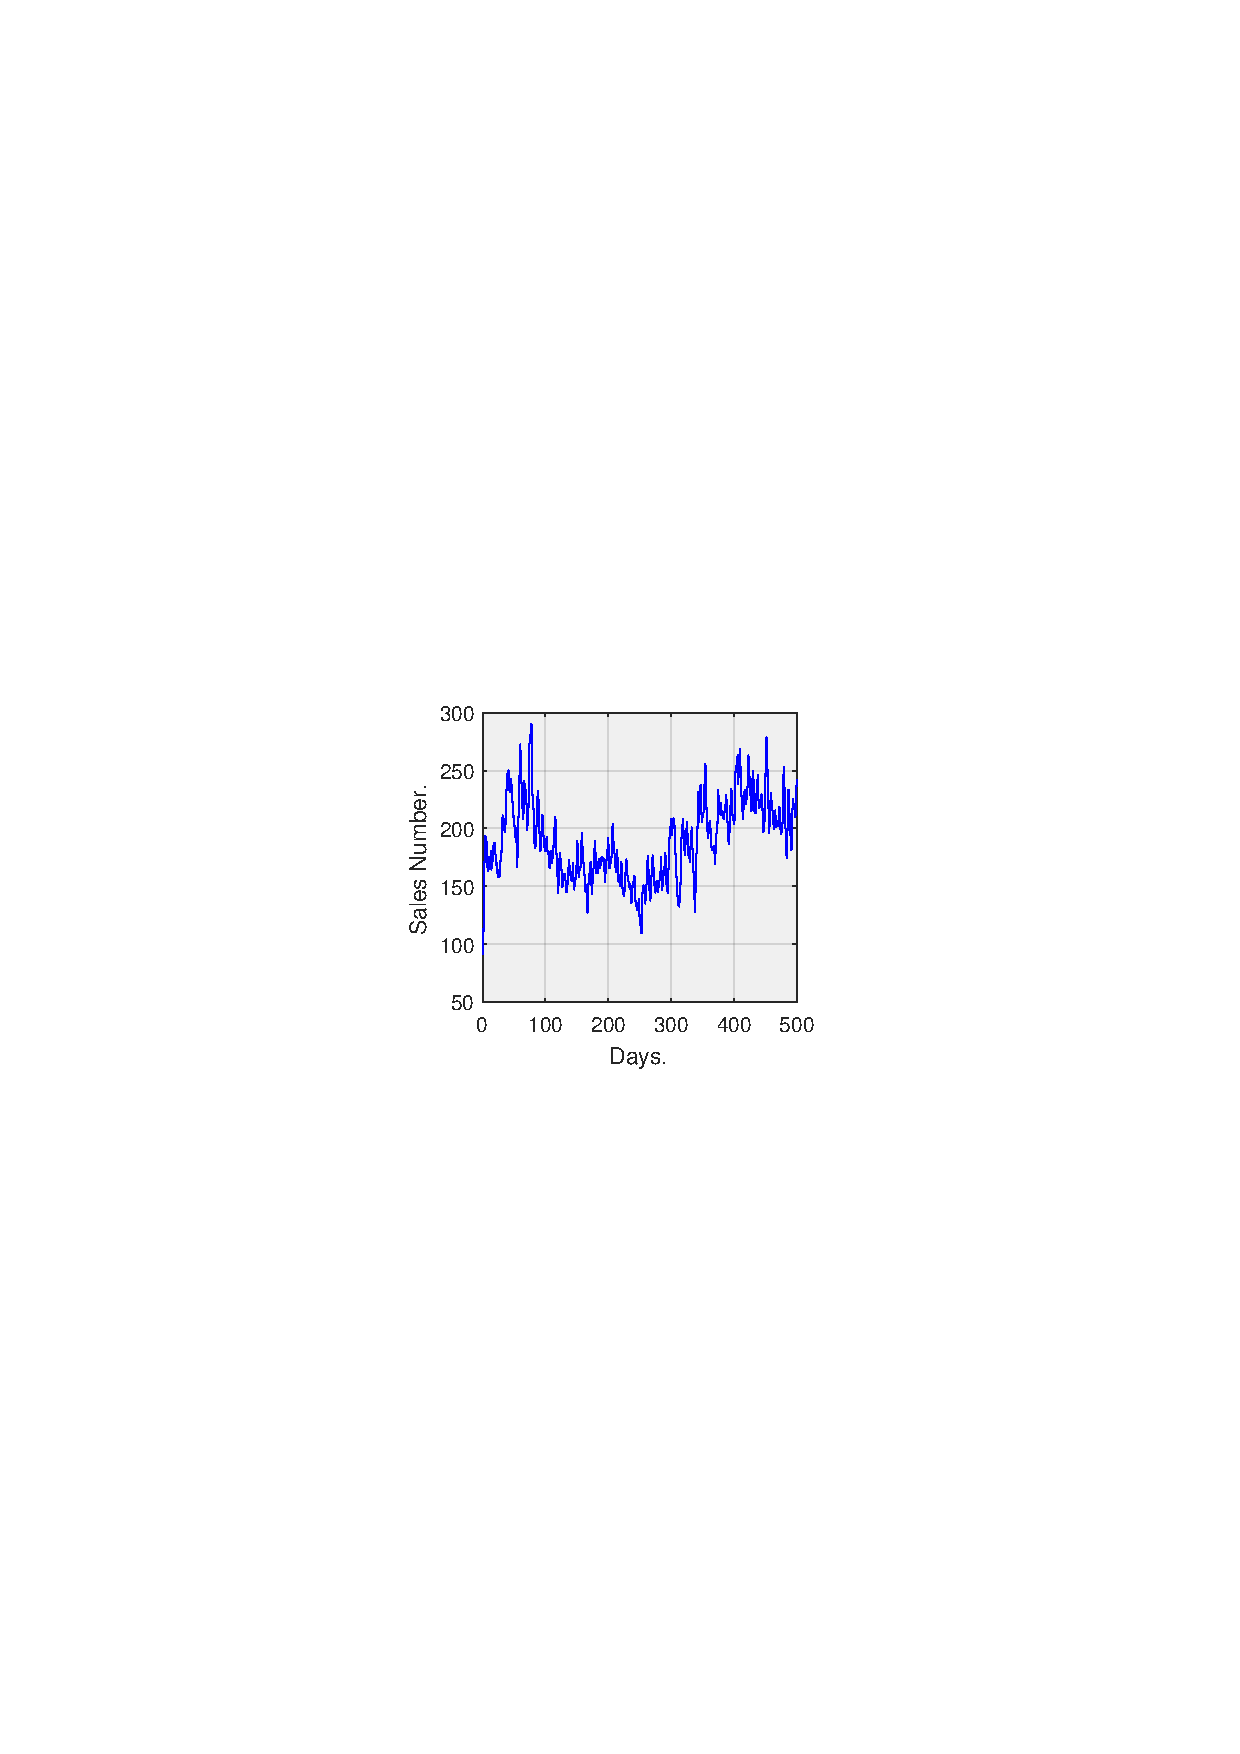
\includegraphics[width=0.33\columnwidth]{chart/day_beauty.pdf}
            \label{day_Beauty}
        }
        %
        \caption{Sales behavior in three Amazon datasets.} 
        \label{day_cmp}
    \end{minipage}
%    \setlength{\abovecaptionskip}{-1pt}
    \vspace{-0.15cm}
\end{figure}


 While some KG-based recommendation methods have modeled temporal information~\cite{kerl, KSR, huang2019explainable}, they mainly use KG data to enhance representation rather 
reasoning over the KG. Their focus is on modeling the interaction sequence for sequential recommendation, rather than the more general temporal patterns as exampled above. It remains underexplored how to model the rich patterns (\eg, seasons, shopping festivals, \etc) that can be inferred from timestamps.  

% Indeed, KG data with temporal information have been widely utilized in 
% recommendation tasks \cite{kerl, KSR, huang2019explainable}. 
% Previous studies mainly utilize KG data to enhance representation rather 
% reasoning over the KG, and mostly 
% focus on previous interaction sequence instead of the specific timestamps. As
% such, they cannot well capture  
% KG structural constraints, and will lack of modeling temporal patterns 
% (\eg, seasons, shopping festivals, \etc) that come with the 
% timestamp.


% 怎么改写这一段, 段段匹配.
%To model temporal patterns inherent in user-item interactions, 
% Therefore, 
% we propose a novel
% {\it \textbf{T}ime-aware \textbf{P}ath reasoning for \textbf{Rec}ommendation}
% (\tkgrec\ for short) method. 
% Our general idea  is to 
In this work, we
frame user-item interactions as time-aware relations. In the example of Figure \ref{intro_exp}, if the reasoning agent is guided by  
% $\bm{(User ,\ Purchase\  in \ Winter\  and\ festival, 
% [?])}$
\textbf{"What items will users purchase in winter and festival?"}
%\footnote{\yyzhao{How to make this expression more precisely?}}
, then 
\underline{Path B} and \underline{Path D}  can be easily inferred.
Nonetheless, it is non-trivial due to 
the following challenges: 
%
% 关系类型不能太多
\textbf{(i) A huge number of timestamps.}
Figure \ref{day_cmp} is based on the Amazon datasets~\cite{HM+2016},  which 
demonstrate user purchasing behaviors, as well as 
the corresponding timestamps over a 500-day period.
As the total number of timestamps is numerous, they cannot be directly 
considered as relation types.
% , and may be time-consuming and space-consuming to 
% obtain the relation embeddings.
%
% 时间距离定义模糊
\textbf{(ii) 	
Ambiguous definition of temporal distance.}
Those timestamps 
% that are close in linear time
do not always suggest similar user behaviors.
%
As illustrated in Figure \ref{day_cmp}, 
the sales of items in the same season tend to be similar in different years,
rather than in different seasons of the same year. 
%
% The performance is similar in other datasets (Figure
% \ref{day_Cell}, \ref{day_Beauty}). 
%
%
% 不平衡的KG.
\textbf{(iii) Different information sources.}
%\footnote{\yyzhao{Maybe the unbalanced KG update frequency shouldn't be 
%mentioned, so I removed it. Is this better?}}
In recommender systems, the interactions between users and items continuously stream in. But the external KG is relatively stable and seldom updated,
%
%\footnote{\yyzhao{Actually interaction won't be updated until the dateset 
%owner 
%publishes it, either. }}
%
which means we couldn't treat them equally 
when performing time-aware path reasoning.



To address the above challenges, 
% we propose a novel
% {\it \textbf{T}ime-aware \textbf{P}ath reasoning for \textbf{Rec}ommendation}
% (\tkgrec\ for short) method. 
% 提出了一个交互时间图谱来帮助进行时序推理.
we integrate the time-aware interactions into KG as a 
heterogeneous information graph (TCKG for short).
%collaborative knowledge graph with time-aware interactions (TCKG
%\footnote{\yyzhao{The name 'TCKG' sounds stupid...}}
% for short) for promoting time-aware path reasoning.
%
We propose a novel
{\it \textbf{T}ime-aware \textbf{P}ath reasoning for \textbf{Rec}ommendation}
(\tkgrec\ for short) method. 
Our method consists of three components.
%
The first one is the time-aware interaction relation extraction 
component.
%
%In this component, in order to ease the different knowledge sources problem,  
%we
%In this component, we
%take the time of \textit{interaction relations} into consideration, while 
%leaving the original KG relations unchanged. 
%%
We apply time series clustering on 
the interaction timestamps
and replace the original interaction relations with clustered relations.
By doing this, we could control the number of relation types, and make the 
extracted relations sensitive to time.
%
More specifically, the timestamp's temporal features consist of statistical and 
structural
discriminative properties, which enables us to measure temporal similarity and 
behavioral pattern similarity.  
%
In the second component, we adopt translational distance learning to 
encode entities and relations in TCKG to obtain
time-aware semantic representation.
%
The third component is the key time-aware path reasoning component.
%
In this component, we shape a personalized time-aware reward 
based on each user's interaction history and recommend time,
which is used to guide the reinforcement learning (RL) reasoner to explore more
precisely.
%% 在想把这一段删掉.... 怪怪的.
%Besides, since there exists implicit temporal dependency between hops in 
%reasoning paths, 
%just like the dependency between words in the sentence translation task, we 
%propose to 
%enhance the state representations with a widely used BLSTM layer in our policy 
%network.
%
%\footnote{\yyzhao{}}
%
%our policy network adopts a widely used bidirectional LSTM to 
%encode
%state vector, which aims to capture the implicit temporal dependence between
%reasoning hops.
%%
%\footnote{\hxie{why specifically mention ``bidirectional LSTM''? need 
%elaborate 
%a little bit to better explain the rationale as well as the 
%novelty?}{Actually, 
%BLSTM is widely used in other nlp tasks. I adopt it just because BLSTM 
%works well in experiment, and the ability of process sequence tasks seems to 
%have something to write about. e.g. "implicit temporal dependence between
%reasoning hops". LOL}}
%


%


%5. 总结贡献以及实验结论.
In summary, the contributions are as follows:

\begin{itemize}
%
\item We design a TCKG to properly integrate the temporal information into 
KG-based recommendation.
To the best of our knowledge, it is the first work to 
introduce time-aware path reasoning
for explainable recommendation.

%\item  To the best of our knowledge, our proposed \tkgrec\ is the first 
%work to 
%% design a TCKG to integrate the temporal information with knowledge graph, and
%introduce time-aware path reasoning method into a recommender system, based on 
%the designed TCKG which integrate the temporal information with knowledge 
%graph.
%
%%\item We design a TCKG to properly integrate the temporal information into 
%%the 
%%knowledge graph under the recommended scenario.

\item We propose a personalized time-aware reward to guide the RL-based 
reasoning agent,
which makes the time-aware reasoning achieve a
more accurate and interpretable  recommendation.

\item We conduct experiments on three real-world datasets, and the results 
demonstrate the effectiveness of \tkgrec\ over several state-of-the-art 
baselines. The codes are available at https://github.com/Go0day/TPRec.


\end{itemize}

%The remainder of this paper is organized as follows. We first present the
%problem formulation in Section~\ref{sec2}, then present the
%rationale and the algorithmic design of \tkgrec\ in Section~\ref{sec:method}. 
%We
%further conduct extensive experiments and present the evaluation results in
%Section~\ref{exper}. We present the related work in
%Section~\ref{sec:related}, and conclude the paper with future works in
%Section~\ref{sec:conclusion}.


\section{Problem Formulation}\label{sec2}
%Before introducing our proposed models, we first formally detail some concepts 
%related to our work.

%Knowledge graph reasoning is the core of making explainable 
%recommendation[PGPR]. 
%In this paper, we consider to add temporal information to the inferred
%multi-hop paths on the KG. Accordingly, the knowledge graph reasoning for 
%explainable recommendation problem can be formulated as follows:
%
%\textbf{Input.} The model input consists of the user set $U$, the item set 
%$V$,

\begin{table*}[t!] 
    \centering
    \caption{Notation and Definitions.}
\begin{tabular}{cc} 
\toprule
\textbf{Notations} & \textbf{Annotation} \\ \hline
$\mathcal{U}$                  & User set                \\
$\mathcal{V}$                  & Global item set                \\ 
$\mathcal{V}_\mathcal{U}$      & The observed interactions between users and items  \\
$\mathcal{V}_\mathcal{U}^T$     & The clustered time-aware interaction set, with $L$ categories \\
$\mathcal{G}_T$                 & Time-aware Collaborative Knowledge Graph \\
$\mathcal{E}^{\prime}$          & The entities in Time-aware Collaborative Knowledge Graph \\
$\mathcal{R}_T$                 & The relations in Time-aware Collaborative Knowledge Graph \\
$T$                             & The interaction timestamp set \\
$\hat{T}$                       & The recommend time \\
$\hat{\mathcal{V}}$             & The recommended item set \\
$\tau_{u, \hat{\mathcal{V}}}$   & The reasoning path set for user $u$ to  item set $\hat{\mathcal{V}}$ \\
$\mathcal{T}$                & Temporal feature space, including statistical features and structural features \\
$r_{kg}$                        & The  external knowledge graph relation set \\
$r_{interact}$                  & The time-aware interaction relation set \\
$\Mat{r}$                       & The embedding of relations            \\
$\Mat{e}_h, \Mat{e}_t$          & The embedding of entities                \\
$\Mat{W}_{t},  \Mat{W}_{\hat{T}}$   & The weight distribution of the Gaussian models at timestamp $t$,\ $\hat{T}$ \\
$\Mat{W}_{h_u}$                 & The time cluster weight distribution of user $u$'s interaction history \\
$k, k^{\prime}, K$                  & The $k$-th reasoning step, state history length $k^{\prime}$ and terminal step \\
$\Mat{s}_k$                     & The state at step $k$ \\
$a_k, \Set{A}_k$                     & The action and action space at step $k$ \\
$g_R(\hat{v} \mid u)$           &  The time-aware based reward for recommended item $\hat{v}$ for user $u$ \\
$\pi\left(\cdot \mid \mathbf{s}_k, \mathcal{A}_{k}(u)\right)$ & The policy network at step $k$ \\
$\hat{c}(\mathbf{s}_k)$         & The value network at step $k$ \\ \bottomrule
\end{tabular}
\label{notation_table}
\end{table*}


\noindent\textbf{Notions:} 
We consider the time-aware path reasoning for KG-enhanced recommendation.
Let denote the user set, the item set, and the observed interactions as $\mathcal{U}$, $\mathcal{V}$, ${\mathcal{V}}_{\mathcal{U}}$, respectively.
Moreover, there exists an external KG storing item properties. Generally, the KG is represented as $\mathcal{G}=\{(h, r, t)  \mid h, t \in \mathcal{E}, r \in \mathcal{R}\}$, where $\mathcal{E}$ represents the set of real-world entities and $\mathcal{R}$ is the set of relation.  
Each triplet $(h,r,t)$ delineates that there exist a relationship $r$ from head entity $h$ to tail entity $t$.
Previous works \cite{multi_modal,kgat} combine the user behaviors and item knowledge as a unified relational graph, termed Collaborative Knowledge Graph (CKG), which is defined as 
$\mathcal{G}_R=\{(h, r, t) \mid h, t \in \mathcal{E}^{\prime}$, $ r \in \mathcal{R}^{\prime}\}$,  where $ \mathcal{E}^{\prime}=\mathcal{E} \cup \mathcal{U}$ and $ \mathcal{R}^{\prime}=\mathcal{R} \cup{\mathcal{V}}_{\mathcal{U}}$. The notations of this work are summarized in Table \ref{notation_table}.
	 
\vspace{5pt}
\noindent\textbf{Reasoning Environment:}
Considering the time-aware interactions instead, we further obtain a Time-aware Collaborative Knowledge Graph (TCKG), which is the environment of time-aware path reasoning.
Specifically, the interaction timestamps are grouped into $L$ groups after time-series clustering, and the interaction relation ${\mathcal{V}}_{\mathcal{U}}$ is extended to $\{\mathcal{V}_{\mathcal{U}}^1, 
\mathcal{V}_{\mathcal{U}}^2, \cdots, \mathcal{V}_{\mathcal{U}}^{L}\}$.
Hence, the TCKG is formulated as $\mathcal{G}_T=\{(h, r, t) \mid 
h, t \in \mathcal{E}^{\prime}, r \in \mathcal{R}_{T}\}$, where 
$ \mathcal{R}_{T}=\mathcal{R} \cup \{ \mathcal{V}_{\mathcal{U}}^1, 
\mathcal{V}_{\mathcal{U}}^2, \cdots, \mathcal{V}_{\mathcal{U}}^{L} \}$.


\vspace{5pt}
\noindent\textbf{Task Description:}
We present the task of time-aware path reasoning for recommendation (TPRec) as follows:
\begin{itemize}
\item \textbf{Input:} Time-aware collaborative knowledge graph $\mathcal{G}_T$;
% \item \textbf{Input:} The model's input consists of the user set 
% $\mathcal{U}$, the item set $\mathcal{V}$,  the observed interactions 
% ${\mathcal{V}}_{\mathcal{U}}$, 
%  the observed interactions' timestamp set $T = \{t_1, t_2, ..., t_n\}$ where 
%  $n$ 
% denotes the total number of timestamps, and the collaborative knowledge graph 
% $\mathcal{G}_R$.

\item \textbf{Output:} Given a user $u$ and a timestamp $\hat{T}$, a recommender model results in an item set $\hat{\mathcal{V}} \subseteq 
\mathcal{V} $ with the corresponding explainable reasoning paths $\tau_{u, 
\hat{\mathcal{V}}}$.  
In particular, for an item $\hat{v} \in \hat{\mathcal{V}}$, 
$\tau_{u, \hat{v}}$ is a multi-hop path, which connects user $u$ with item $\hat{v}$ to explain why $\hat{v}$ is suitable for $u$: 
$\tau_{u, \hat{v}}=[u 
\stackrel{r_{1}}{\longrightarrow} e_{1} \stackrel{r_{2}}{\longrightarrow} 
\ldots \stackrel{r_{k-1}}{\longrightarrow} e_{k-1} 
\stackrel{r_{k}}{\longrightarrow} \hat{v}]$, where $e_{i-1} 
\stackrel{r_{i}}{\longrightarrow} e_{i}$ represents $(e_{i-1}, r_i, e_i) \in 
\mathcal{G}_T, i \in [k]$.

\end{itemize} 

% 可能一些, 比如类间距离大类内距离小的假设应该放在这里.
% 还有那个多跳推理能够成功的假设.






\section{Methodology}
\label{sec:method}

%We now present the proposed TER model, which uses temporary information for 
%explanation recommendation.

%============================================================================
%
%We now describe the proposed \tkgrec\ in details.
% Figure \ref{pipeline} sketches the model's architecture, which 
%consists of four main modules: 
%%
%\textbf{(1) Time-aware interact} 
%module, which constructs TKG by the interaction time-series 
%clustering mechanism and encodes the TKG to get temporal representation;
%%
%\textbf{(2) Time-aware Path Reasoner} 
%module, which innovatively leverages temporal information as guiding signals 
%for generating personalized recommendation; 
%%
%\textbf{(3) Temporal Ranking Recommendation} 
%module, which aims at ranking the predicted items from the trained reasoner to 
%get a temporal order recommendation.
In this section, we introduce the proposed \tkgrec\ in detail.
The overall framework of time-aware path reasoning is shown in Figure 
\ref{pipeline}.
%
Our approach is able to effectively fuse temporal information into knowledge 
graph and leverage a RL framework for recommendation.
In what follows, we start with 
\textbf{Time-aware Interaction Relation Extraction} 
to construct TCKG, and use \textbf{Time-aware representation learning} 
to generate entities and relations representations.
Then we present \textbf{Time-aware Path Reasoning} and \textbf{Model Prediction} to reason over TCKG for recommendation.

%============================================================================



\subsection{Time-aware Interaction Relation Extraction}\label{tire}
Clearly, how to deal with the dynamic characteristics of user-item interactions is of crucial importance in our task.
However, simply treating the interaction timestamps as auxiliary features might limit the potential of time-aware reasoning, due to the following challenges:
(1) As the timestamps are usually numerous \cite{datasetAmazon}, directly attaching them with user behaviors might cause meaningless features, such as purchase\_20150101 and purchase\_20150102, thus enlarging the feature space dramatically and losing the periodic semantics of timestamps.
(2) The interaction graph and knowledge graph come from heterogeneous sources, and thus are hardly updated synchronously --- that is, the interactions are usually dynamic, while the item knowledge (\eg, category, brand) is fixed over different timestamps.

To solve these challenges, we first consider the temporal and behavioral characteristics of interactions by projecting the timestamps into a temporal feature space $\mathcal{T}$.
It encodes temporal statistical and temporal structural features of interaction timestamps.
We then group the interaction timestamps $T = \{t_1, t_2, \cdots, t_n\}$ into $L$ categories, and then extend the single interaction type into $\mathcal{V}_{\mathcal{U}}^T = \{ \mathcal{V}_{\mathcal{U}}^1, \mathcal{V}_{\mathcal{U}}^2, \cdots, \mathcal{V}_{\mathcal{U}}^{L} \}$.
After that, the temporal user-item graph can be seamlessly integrated with relatively static KG based on the item-entity alignment set, and finally get the TCKG we need.
The extraction process is illustrated in Figure \ref{clu}.


% we first group the interaction timestamps $T = \{t_1, t_2, \cdots, t_n\}$ into $l$ categories, and then extend the single interaction type into $\mathcal{V}_{\mathcal{U}}^T = \{ \mathcal{V}_{\mathcal{U}}^1, \mathcal{V}_{\mathcal{U}}^2, \cdots, \mathcal{V}_{\mathcal{U}}^{l} \}$.
% Thereafter, we consider the temporal and behavioral characteristics of interactions by projecting the timestamps into a feature space $\mathcal{T} \in \mathbb{R}^m$, where $m$ indicates the space dimension.
% It encodes temporal statistical and temporal structural features of interaction timestamps.
% We illustrate the extraction process in Figure \ref{clu} and and elaborate it in the next sections. 



% Directly treating the timestamp as auxiliary features of the entity or 
% relation is suboptimal for path reasoning, due to the 
% following challenges:
% (1) As the timestamps are usually numerous \cite{datasetAmazon}, simply attaching the original relation with timestamps might loss the periodic characteristics and lead to meaningless features.
% (2) More importantly, the user-item bipartite graph and knowledge 
% graph come from different sources and are hardly updated synchronously --- that is, the interactions are dynamic, while the item knowledge (\eg, category, brand) is static over different timestamps.
% % The interaction of users purchasing items is happening all the time, and every interaction occurs with explicit behavioral intentions. But the external knowledge graph is derived from existing public KGs or extracted from 
% % the local business information network (\eg, category, brand), which is 
% % difficult to capture complete and specific timestamps.
% %
% Here, we propose TCKG to emphasize the dynamics of interactions.
% In particular, we divide the timestamps of interactions $T = \{t_1, 
% t_2, \cdots, t_n\}$ into $l$ categories, and obtain the time-aware interaction relations $\mathcal{V}_{\mathcal{U}}^T = \{ \mathcal{V}_{\mathcal{U}}^1, \mathcal{V}_{\mathcal{U}}^2, \cdots, \mathcal{V}_{\mathcal{U}}^{l} \}$.
% We visualize the extraction process in Figure \ref{clu}.
 
% To capture the temporal and behavioral characteristics of interactions, we identify two types of discriminative features: \textit{statistical} features and 
% \textit{structural} features.
% %
% These two types of features 
% %are widely used in unlabeled time-series data \cite{features_time},
% will represent 
% interaction timestamp set $T = \{t_1, t_2, ..., t_n\}$
% and compose our temporal feature space  $\mathcal{T} \in \mathbb{R}^m$, 
% where $m$ indicates the 
% dimensionality of the space.
% The details will be shown below.



\subsubsection{\textbf{Temporal Statistical Features}}
Before clustering timestamps, we project them into a feature space.
Specifically, the statistical features are considered to capture some time rules like seasonal changes, periodic purchases \cite{liao2005clustering}.
Hence, for a specific timestamp $t$, its statistical feature is formally summarized as:
\begin{equation}
    \boldsymbol{f}_{stat} =year(t)|| season(t) || month(t) || week(t) \cdots,
\end{equation}
where $\boldsymbol{f}_{stat}$ encodes the year,  season, month, week, and other statistical characteristics of $t$ and concatenates them together, where $||$ is the concatenate operator.


\begin{figure}[tb]
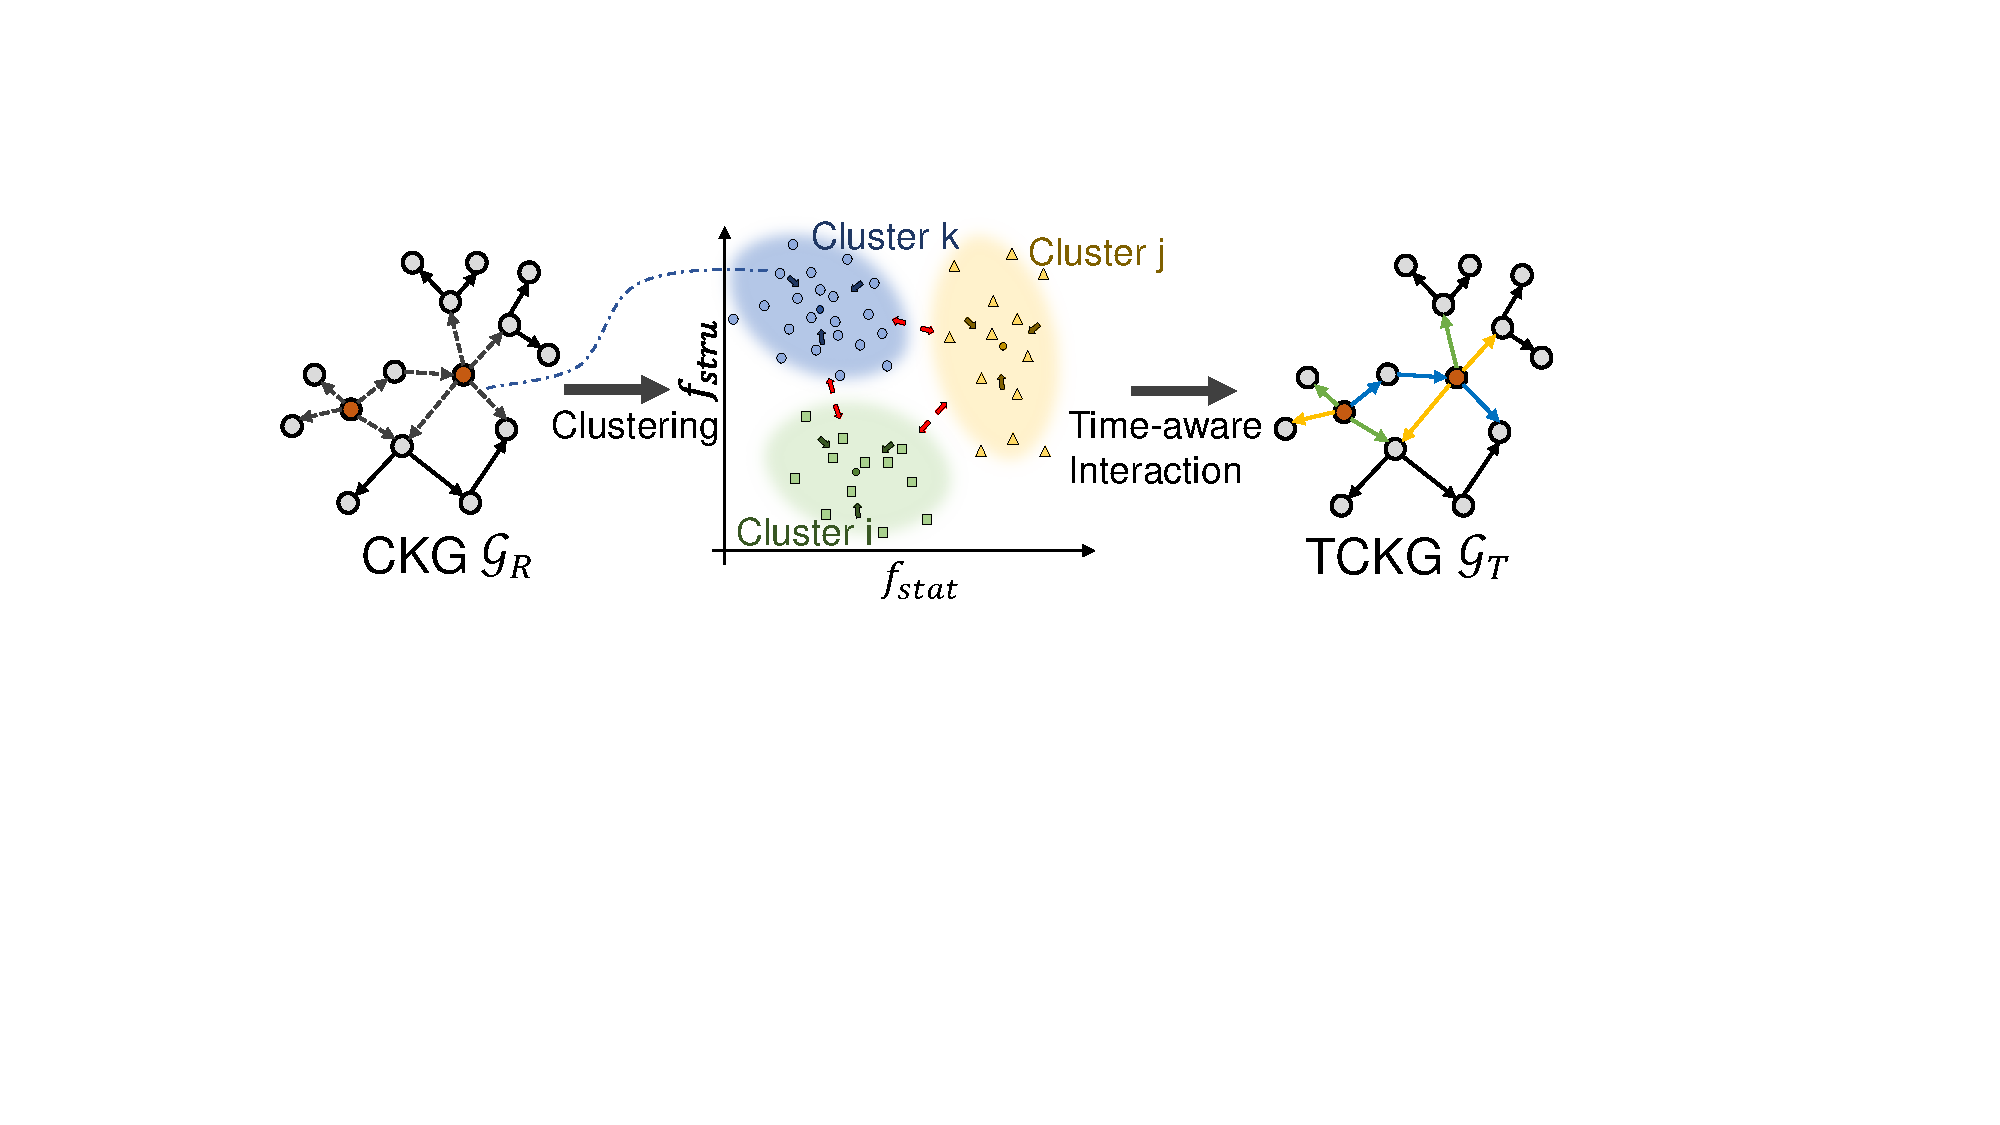
\includegraphics[width=0.85\columnwidth]{chart/clu.pdf}
\caption{Process of time-aware interaction relation extraction. Each 
interaction relation's (dashed edge) timestamp will be mapped into temporal 
feature space 
$\mathcal{T}$ and clustered. Different colored edges (\eg, blue, yellow, green) in TCKG represent 
different clustering results. }
\label{clu}
\end{figure}

\subsubsection{\textbf{Temporal structural features}}
Beyond the statistical features, we also exploit the structural features to delineate the characteristics of user behaviors, which measures the purchase propensity (\eg, shopping festival) at timestamp $t$.
More formally, we define the structural feature of $t$ as:
\begin{equation}
	\boldsymbol{f}_{stru} = z_{gap}'(t) || z_{gap}''(t),
\end{equation}
where $z_{gap}'(t)$ is the first-order structural feature, which measures the trend of interaction number in the current $gap$ time, compared with that in the past $gap$; $gap$ represents the granularity of window period, which can be set as 30 (\ie, month), or 1 (\ie, day); analogously, $z_{gap}''(t)$ denotes the second-order structural feature and models the momentum of interaction trend.
More formally, $z_{gap}'(t)$ and $z_{gap}''(t)$ is defined as:
% \begin{equation}
% 	 z_{gap}'(t) = \frac{\sum_{i=t-gap}^{t}z(i) - \sum_{i=t-2gap}^{t-gap}z(i)}{gap}
% \end{equation}
\begin{align}  \label{z_p}
	 z_{gap}'(t) &= \frac{\sum_{i=t-gap}^{t}z(i) - \sum_{i=t-2gap}^{t-gap}z(i)}{gap},\ & z_{gap}''(t) &= \frac{\sum_{i=t-gap}^{t}z_{gap}'(i) - \sum_{i=t-2gap}^{t-gap}z_{gap}'(i)}{gap},
\end{align}

where $z(i)$ is the interaction number happened on timestamp $i$, and we replace $z(i)$ with $z_{gap}'(i)$ in Eq. \ref{z_p} to calculate $z_{gap}''(t)$.
For those timestamp $t$ has less than $2gap$ historical interactions, their historical information is not enough to calculate $z_{gap}'(i)$.
In that case, we padding their corresponding features with the nearest timestamp's temporal structural feature. The same goes for $z_{gap}''(t)$.
% We replace it with the nearest timestamp
% As a result, $\boldsymbol{F}^{\prime \prime}$ reflects the first-
In this work, we set the gap as 90 (\ie, season), 30 (\ie, month), 7 (\ie, week), 1 (\ie, day) and simply concatenate them as temporal structural features.

Thereafter, we combine these two features together as the temporal feature space $\mathcal{T} \in \Space{R}^m$ for timestamp $t$:
\begin{equation}
	\mathcal{T} = \boldsymbol{f}_{stat} \ || \ \boldsymbol{f}_{stru},
\end{equation}
where $m$ is the feature dimension.


% Before grouping timestamps into categories, we map them into temporal feature 
% space 
% $\mathcal{T}$. The statistical features are 
% expected \cite{liao2005clustering} to capture some time rules like seasonal 
% changes, periodic 
% purchases, 
% \etc\ 
% The statistical features can be formally summarized as:
% \begin{equation}
% 	\boldsymbol{F}^{\prime} = f_{stat}(t)
% 	\end{equation}
% 	where $t$ represent an interaction timestamp, and $f_{stat}(t)$ means 
% 	encode 	the 
% 	timestamp $t$ with statistical features. 
% 	\ie, the function $f_{stat}(\cdot)$ will extract 
%  the year, month, season, week and other statistical characteristics of 
% each timestamp $t$, and concatenate them together after encoding. In particular, 
% $f_{stat}$
% can be formulated as:
% \begin{equation}
% 	f_{stat}(t) = year(t) \| season(t) \| month(t) \| ... 
% 	\end{equation}
% 	where $\|$ means concatenate operator.



% \subsubsection{Temporal structural features}
% Beyond the statistical features, we exploit structural features to capture 
% the characteristics of users' shopping behavior.
% Similarly, the statistical features can be formulated as:
% \begin{equation}
% 	\boldsymbol{F}^{\prime \prime} = f_{stru}(t)
% 	\end{equation}
% More specifically, $f_{stru}(t)$ contains 
% the first- and second-order features
% of time-interact function $z(t)$:
% \begin{equation}
% 	f_{stru}(t) = z_{gap}^{\prime}(t)  \| 
% 	z_{gap}^{\prime \prime}(t)
% 	\end{equation}
% where time-interact function $z(t)$ is the interaction number $n$ occured on 
% timestamp $t$, and $z_{gap}^{\prime}(n)$ model the trend of $n$ in current 
% $gap$ 
% time relative to past $gap$ time:
% \begin{equation}
% 	 z_{gap}^{\prime}(t) = \frac{\sum_{i=t-gap}^{t}z(i) 
% 	 - \sum_{i=t-2gap}^{t-gap}z(i)}{gap}
% 	\end{equation}\label{z_p}
% where $gap$ represents time granularity, which can be 30 (\ie month), 90 (\ie 
% season) or 1 (\ie day), \etc\ $z_{gap}^{\prime \prime}(t)$ models the momentum 
% of interaction trend, and can be calculated by replacing $z(i)$ in Equation 
% \ref{z_p} with $z_{gap}^{\prime}(t)$.

% These two types of features will compose our time-aware feature space 
% $\mathcal{T} \in 
% \mathbb{R}^m$:
% \begin{equation}
% 	\mathcal{T} = \boldsymbol{F}^{\prime} \|  \boldsymbol{F}^{\prime \prime}
% 	\end{equation}

\subsubsection{\textbf{TCKG Construction}}
Having mapped the timestamp to the temporal feature space, we now construct the relation of time-aware interaction.
Here we adopt a time-series clustering method, Gaussian Mixture Model (GMM) \cite{gmm}, on the timestamp set $T$, so as to reduce the timestamp numbers and discretize them into group values.
We leave the exploration of other clustering methods, such as K-means \cite{kmeans}, DBSCAN \cite{ester1996density}, and Mean-shift \cite{meanshift}, in future work.

Specifically, we hire $L$ Gaussian models. For the timestamp $t$ with its temporal feature, we can get the probability $w_{l}$ of being generated by the $l$-th Gaussian model.
As such, the interaction relation $r_t$ on timestamp $t$ can be obtained as follows:
\begin{equation}\label{relation_cluster_2}
	r_t \leftarrow \Space{I}_{max(\Mat{W}_{t})}(\Mat{W}_{t}) {\mathcal{V}_{\mathcal{U}}^T} \ ,
\end{equation}
where $\Mat{W}_{t} = [w^{1}_t, w^{2}_t, \cdots, w^{L}_t]^{\mathsf{T}}$ indicates the $t$-specific probability distribution derived from the Gaussian models;
${\mathcal{V}}_{\mathcal{U}}^T = [\mathcal{V}_{\mathcal{U}}^1, \mathcal{V}_{\mathcal{U}}^2, \cdots, \mathcal{V}_{\mathcal{U}}^{L}]$ is the time-aware interaction relation set, where $\mathcal{V}_{\mathcal{U}}^{l}$ is the $l$-th clustered relation.
Equation \eqref{relation_cluster_2} replaces $r_t$ with the most probable relation in ${\mathcal{V}}_{\mathcal{U}}^T$.
The number of time clusters $L$ is determined by the Bayesian Information Criterion (BIC) \cite{bic}, which is adjusted adaptively for different datasets.


Through the above extract process, we are able to project each observed interaction with timestamp into the same time-aware feature space, and divide all timestamps into weighted $L$ clusters by GMM.
The clustering assignments are used to replace the original interaction relations in CKG and finally convert CKG into TCKG.


% \subsubsection{TCKG Construction}
% Having mapped  the timestamp set $T$ to the time-aware feature space 
% $\mathcal{T}$, 
% we need to construct a time-aware interact relation based on those information.
% Here we adopt a time-series clustering mechanism on timestamp set $T$
% because the total number
% of timestamps is numerous and need to be bucketized into group values.
% % 表示很多聚类方法也行但是我们用的是GMM做.
% The clustering process can be modeled by K-means \cite{kmeans}, DBSCAN 
% \cite{ester1996density}, or 
% Mean-shift \cite{meanshift}, \etc\
% Intuitively, we integrate a simple but effective Gaussian Mixture 
% Model (GMM) \cite{gmm} to cluster time data. 



% Especially, for each $i$-th time vector 
% $\boldsymbol{t}_i \in \mathbb{R}^m$, we can get the probability $w_i(k)$ of 
% being generated by the $k$-th Gaussian model (the total amount is $l$). The 
% interaction relation 
% $\boldsymbol{r}_{t_i}$ on $t_i$  can be expressed as follows:
% \begin{equation}
% 	\boldsymbol{r}_{t_i} \leftarrow 
% 	\mathbb{I}_{max(\boldsymbol{w}_i)}(\boldsymbol{w}_i)
% 	\boldsymbol{R}_L^\intercal, \label{relation_cluster_2}
% 	\end{equation}
% where $\boldsymbol{w}_i = [w_i(1), w_i(2), ..., 
% w_i(l)]$ indicates the probability of $\boldsymbol{t}_i$ for each
% Gaussian model, and $\boldsymbol{R}_L = [r_{1}, 
% r_{2}, ..., r_{l}]$ is the extended relation set clustered 
% by GMM where $r_{l}$ is the $l$-th clustered relation. 
% Equation (\ref{relation_cluster_2}) means replacing $\boldsymbol{r}_{t_i}$ with 
% the most 
% probable relation in $\boldsymbol{R}_L$. 
% The number of time clusters $l$ is determined 
% by the Bayesian Information Criterion
% (BIC) \cite{bic},  
% which is adjusted adaptively for different datasets. 
	

% Therefore, each observed interaction with timestamp could be projected into  
% time-aware feature space 
% $\mathcal{T}$, and then be divided into weighted $l$ clusters by GMM model. 
% Those clustered result will replace the original interaction relations in CKG 
% and finally contributes to constructing TCKG.

\begin{figure}[tb]
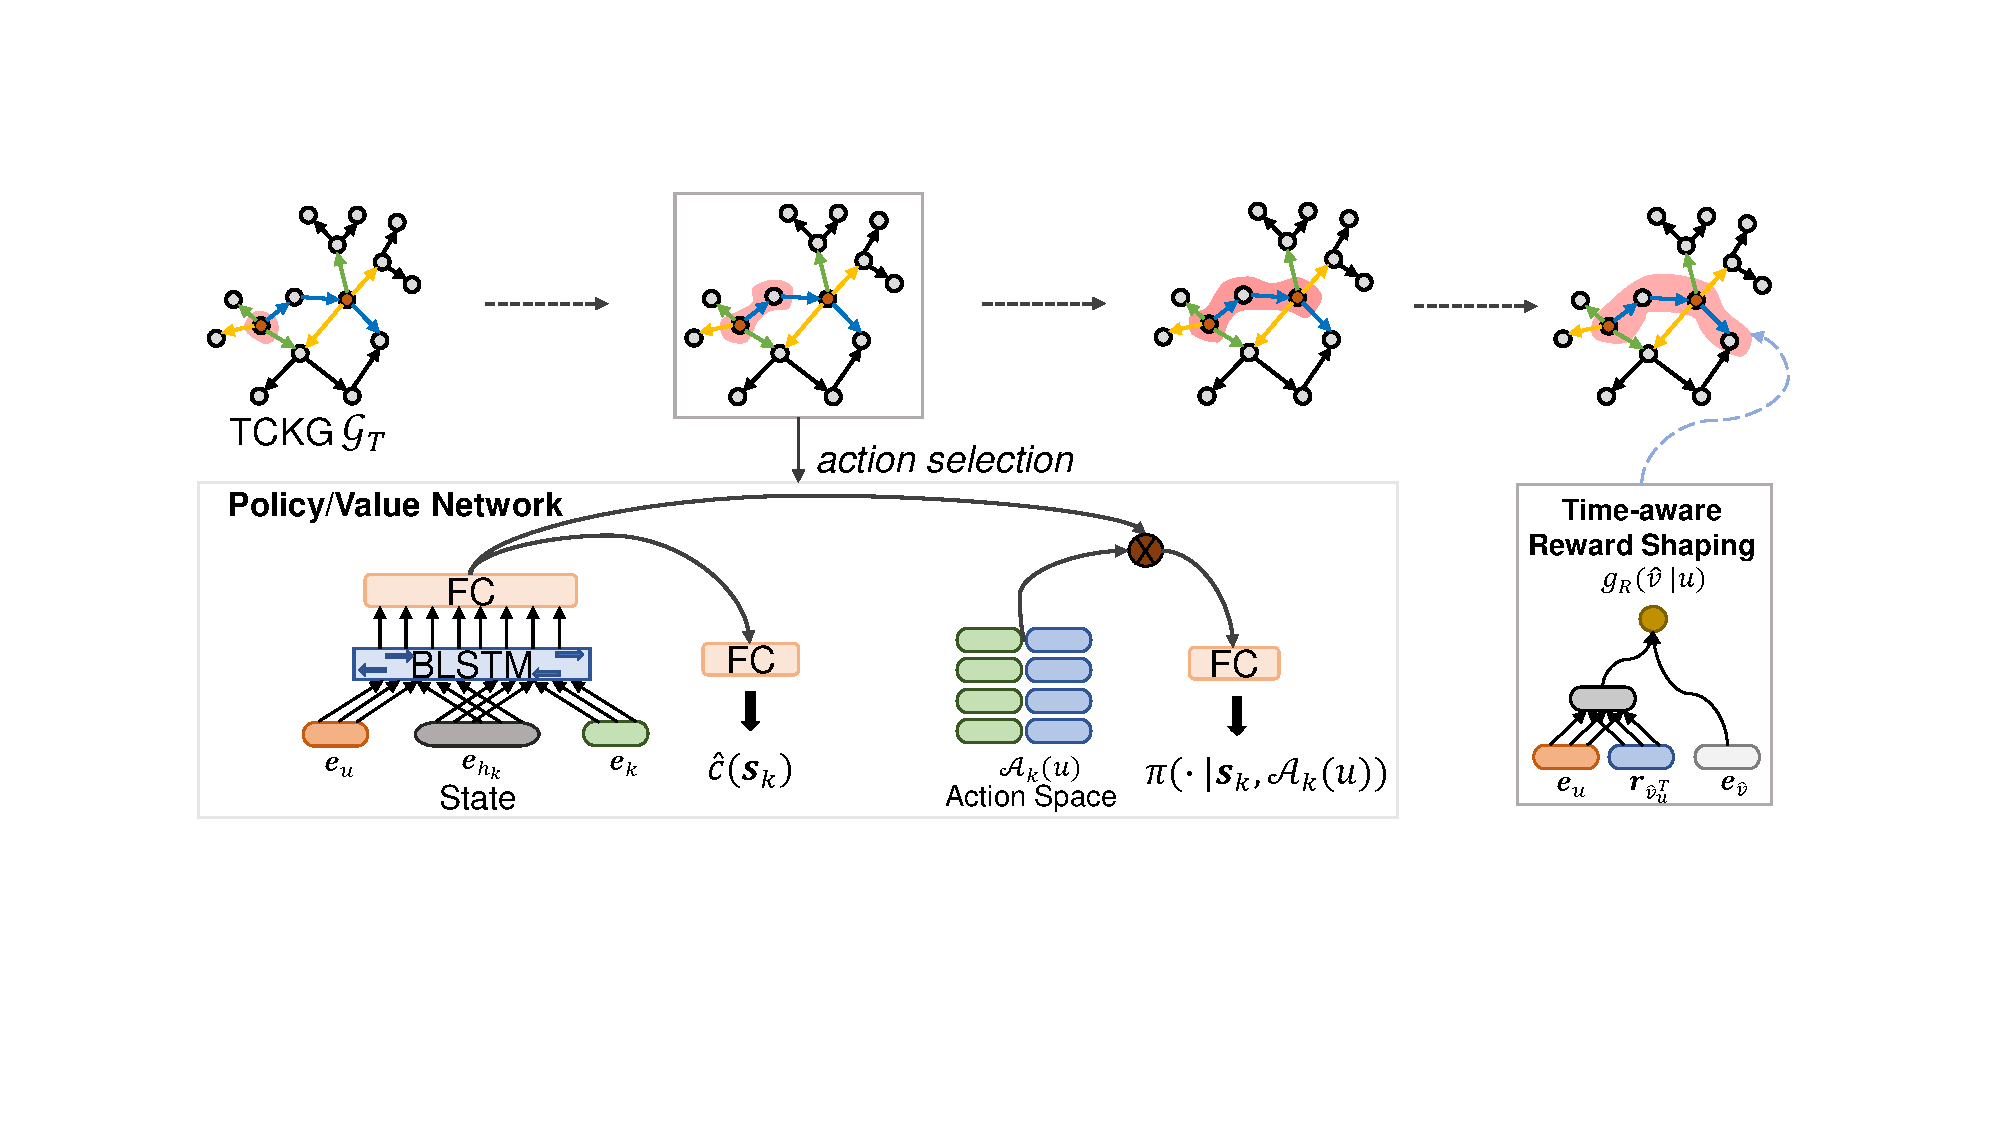
\includegraphics[width=\columnwidth]{chart/pipelineMH.pdf}
\caption{ Overall training approach of the proposed \tkgrec\ model.
		For a user $u$ at each time step $k$, as shown in the pink shaded part of TCKG, the agent chooses the next hop based on the temporal constraint, which samples a  
		link $a_k$ according to 
		$\pi\left(\cdot \mid \mathbf{s}_k, \mathcal{A}_{k}(u)\right)$.
		The agent receives a reward $g_R(\hat{v} \mid u)$  when stopped at an item 
		$\hat{v}$. The pink shaded path starts at user $u$ and ends at item $\hat{v}$, showing why our \tkgrec\ model recommends $\hat{v}$ to $u$.
		%
%		Framework overview of the proposed \tkgrec\ model. 
%				The algorithm aims to learn a policy that navigates from
				}
		\label{pipeline}
\end{figure}



\subsection{Time-aware Representation Learning}\label{trl}
Having constructed TCKG, we aim to learn representations for entities and relations by exhibiting the structural and temporal information.
In particular, the KG relations (defined as $r_{kg}$) require the entity representations to meet the structural constraints and maintain the semantics, while the time-aware interaction relations (defined as $r_{interact} \in {\mathcal{V}}_{\mathcal{U}}^T $) encourage the relation affinity within the same categories compared to that of different categories.



Towards this end, we employ the widely-used knowledge graph embedding method, TransE \cite{transE}, on TCKG.
To be more specific, for a given TCKG triplet $(h,r,t)$, it represents head entity $h$, relation $r \in \{r_{kg} \cup r_{interact}\}$ 
% which includes external KG relation $r_{kg}$ and interact relation $r_{interact}$
, and tail entity $t$ with $d$-dimension embeddings, \ie, $\Mat{e}_{h}$, $\Mat{r}$, $\Mat{e}_{t}$ $\in \mathbb{R}^d$.
These embeddings follow the translational principle: $\Mat{e}_h + \Mat{r} \approx \Mat{e}_t$.
Hence,  for a given triplet $(h, r, t)$, the scoring function is defined as the distance between $\Mat{e}_h + \Mat{r}$ and $\Mat{e}_t$, \ie,
\begin{equation}\label{trans}
	g_{r}({h},{t})=\|\Mat{e}_h+\Mat{r}-
	\Mat{e}_t\|_2^2 .
\end{equation}
A smaller score $g_{r}(h, t)$ suggests that the fact $(h, r, t)$ is more likely to be true, and vice versa. 
We employ the pairwise loss function to train the TCKG embeddings, which accounts for the relative order between the valid triplets and broken ones:
\begin{equation}\label{eqtranse}
    \Lapl_{tckg}=\sum_{\left(h, r, t, t'\right) \in \Set{S}}-\ln\sigma\left(g_{r}({h},{t}') - g_{r}({h},{t})\right)
\end{equation}
where $\Set{S} = \{(h, r, t, t') | (h, r, t) \in \Set{G}_T, (h, r, t') \notin \Set{G}_T\}$, and $ (h, r, t')$ is collected with the tail $t$ replaced by a random entity $t'$; 
$\sigma(\cdot)$ is the sigmoid function. 
This loss serves as a constraint that injects the structural and temporal information into representations, thus preserving the semantics of entities and relations.



% Having constructed the TCKG, we learn 
% representations for entities and relations by jointly considering inherent 
% graph structure and temporal information.
% %
% Therefore, our learning procedure of TCKG embedding comes from \textbf{two} 
% signals: (i) 
% \textbf{Original KG relations}, which makes embedding meet the
% semantic and structural constraints; and (ii) \textbf{Time-aware interaction 
% relations}, 
% which reduces the distances between time-aware relations
% $\mathcal{V}_{\mathcal{U}}^T$ of the same categories and increases the distances
% between the relations of different categories. 


% According to former Section \ref{tire}, our TCKG's relation types 
% $\mathcal{R}_T$ are 
% composed of two categories: original KG relations $r_{kg} \in 
%  \mathcal{R}$ and time-aware interaction relations  $r_{interact} \in \{ 
%  \mathcal{V}_{\mathcal{U}}^1, 
%   \mathcal{V}_{\mathcal{U}}^2, 
%   ..., \mathcal{V}_{\mathcal{U}}^{l} \}$. Although they are both relation types 
%   in TCKG, those embedding distances between $\boldsymbol{r}_{kg}$ and 
%   $\boldsymbol{r}_{interact}$ need to be different. 
% %
% For example, assuming that there are relations $\{r_{a1}, r_{a2}, r_{b1}, 
% r_{b2}\}$ extracted from relations $A$ and $B$. 
% In addition to be encoded by translational distance, furthermore, the distance 
% of
% relation embeddings extracted from the same relation type should be smaller 
% than those from different relation types, \eg, $ \text{d}(\boldsymbol{r}_{a1}, 
% \boldsymbol{r}_{a2}) \leq 
% \min(\text{d}(\boldsymbol{r}_{ai}, \boldsymbol{r}_{bj}))$, $\text{where} \  
% i,j=1,2$, and $\text{d}(\cdot)$ measures distance. 

% We employ the translational scoring function 
% \cite{transE}, 
% a widely used embedding method, on TCKG. To be more specific, it represents 
% both entities and relations in $d$-dimension 
% vector space, \ie, $\boldsymbol{e}_h, \boldsymbol{e}_t, \boldsymbol{r} \in 
% \mathbb{R}^d$, and 
%  makes embeddings follow the translational principle: $\boldsymbol{e}_h + 
%  \boldsymbol{r} \approx \boldsymbol{e}_t$, where $\boldsymbol{e}_h, 
%  \boldsymbol{e}_t$ are the head and tail entity embeddings, and 
%  $\boldsymbol{r} \in \{ 
%  \boldsymbol{r}_{kg} \cup \boldsymbol{r}_{interact}  \}$ 
%  is the relation embedding.
%  %
%  Hence,  for a 
%  given triplet $(h, r, t)$, the scoring 
%  function is defined as the 
%  distance between $\boldsymbol{e}_h + 
%   \boldsymbol{r}$ and $\boldsymbol{e}_t$, \ie,
% 	 \begin{equation}
% 	g_{r}({h},{t})=\|\boldsymbol{e}_h+\boldsymbol{r}-
% 	\boldsymbol{e}_t\|_2^2 ,
% 		 \end{equation} \label{trans}
%  A larger score $g_{r}(h, t)$ suggests that the fact $(h, r, t)$ is more likely 
%  to 
%  be true, and vice versa. 
 %
 %
%  In this way, the original KG relations $r_{kg}$ will be directly encoded by 
%  translational constraint.
% % as 
% % translational representation, because their positions in TCKG are still in 
% % their original places.
%  %
%  As to time-aware interaction relations $r_{interact}$, those relations 
%  extracted  from the 
%  same  interaction relation connect with same head entity types and tail entity 
%  types.  Therefore, the distance of their  
%  representation are smaller than those extracted from different interaction 
%  relation.
%  % 
%  %
%  The training of TCKG embedding considers the relative 
%  order between valid triplets and broken ones, and encourages
%  their discrimination through a pairwise ranking loss:

% \begin{equation}\label{eqtranse}
% \mathcal{L}_{tckg}=\sum_{\left(h, r, t, t^{\prime}\right) \in \mathcal{S}}-\ln 
% \sigma\left(g_{r}({h},{t}^{\prime}) - g_{r}({h},{t})\right)
% \end{equation}
% where $S = \{(h, r, t, t^{\prime}) | (h, r, t) \in \mathcal{G}_T, (h, r, 
% t^{\prime}) \notin \mathcal{G}_T\}$, and $ (h, r, t^{\prime})$ is collected 
%  with the tail $t$ replaced by a random entity $t^{\prime}$.
% $\sigma(\cdot)$ is the sigmoid function. 
% % original KG relations 因为仍然保留了原有的状态, 因此嵌入学习不变.
% % time-aware interaction relations, 由相同interaction提取出的relation之间,头尾实体
% %类别相似, 因此尽管它们在TCKG中属于不同的relation type, 
% %它们的distance会比不同interaction提取的relation更远. 因此完成我们的time-aware 
% %representaion.
% This loss serves as a 
% constraint signal, injecting the direct connections and temporal information 
% into representations, and 
% thus increases the semantics in the embedding .




%
%\subsubsection{Metric Learning.} 
%According to former Section \ref{tire}, our TKG's relation types are 
%composed of two categories: original KG relations $\mathcal{R}$ and temporal 
%classified relations $\mathcal{R}_T$. Although they are both relation types in 
%TKG, those 
%embedding distances between them need to be different. 
%%
%For example, assuming that there are relations $\{a_1, a_2, b_1, b_2\}$ 
%extracted from 
%relations $A$ and $B$. 
%In addition to be encoded by translational distance, furthermore, the distance 
%of
%relation embeddings extracted from the same relation type should be smaller 
%than those from different relation types, \eg, $ \text{d}(a_1, a_2) \leq 
%\min(\text{d}(a_i, b_j))$, $\text{where} \  i,j=1,2$, and $\text{d}(\cdot)$ 
%measures 
%distance. 
%
%In this way, those entities and relations can still encode their original 
%type  
%information into their embedding after being clustered by time, which couples 
%temporal information with types connection to achieve richer 
%representation.
%
%
%
%In order to make Euclidean distances between feature vectors from different 
%classes larger than that from the same class, inspired by 
%\cite{triloss},  
%we set TriHard loss to constraint:
%	\begin{equation}\label{eqtri}
%	\mathcal{L}_{T H}=\sum_{sa\in D, p_{h}, 
%	n_{h}}\left[\text{d}\left(\boldsymbol{r}_{sa}, 
%	\boldsymbol{r}_{p_h}\right)-\text{d}\left(\boldsymbol{r}_{sa}, 
%	\boldsymbol{r}_{n_h}\right)+\alpha\right]_{+}(\alpha>0)
%	\end{equation}
%where $\text{d}(x,y)$ represents the Euclidean distance between $x$ and $y$, 
%$\boldsymbol{r}_{sa} 
%\in \mathbb{R}^d$ are relation embedding vectors of 
%samples in mini-batch $D$, $\boldsymbol{r}_{p_h}, \boldsymbol{r}_{n_h} \in 
%\mathbb{R}^d$ are relation embedding vectors of the hardest positive and 
%negative samples towards anchors within $D$, and $\alpha$ is the margin. It 
%makes 
%the hardest relation triplets 
%more soft and various, and simultaneously solves the distance problem by 
%making 
%the anchor converge to 
%local minima.
%
%In addition to keeping the embeddings of different classes separable, 
%\cite{centloss} is utilized
%here for minimizing the intra-class variations, as follows:
%	\begin{equation}\label{eqcent}
%	\mathcal{L}_{C}=\frac{1}{2} 
%	\sum_{i=1}^{D}\left\|\boldsymbol{r}_{i}-\boldsymbol{c}_{k}\right\|_{2}^{2}, 
%	\end{equation}
%where $\boldsymbol{r}_i \in \mathbb{R}^d$ denotes the $i$-th clustered 
%relation, belonging to $k$-th relation type(\eg, $purchase\_i$ for 
%$purchase$). 
%Besides, 
%$\boldsymbol{c}_k \in 
%\mathbb{R}^d$ denotes the $k$-th relation cluster center embedding.
%
%
%Finally, we obtain the object function to learn Equations 
%(\ref{eqtranse}), (\ref{eqtri}) and (\ref{eqcent}) jointly, as 
%follows:
%	\begin{equation}\label{joint}
%	\mathcal{L}_{TKGE} = \mathcal{L}_{KG} + \lambda \mathcal{L}_{TH} + \eta 
%	\mathcal{L}_C, 
%	\end{equation}
%where scalars $\lambda$ and $\eta$ are used to balance the three loss 
%functions. This module models the entities and relations on the granularity of 
%triplets, working as a regularizer and injecting the temporal connections into 
%semantic representations, which can increase the temporal representation 
%ability of the model.
%
%%1. time-aware feature extraction，我觉得需要着重描写这部
%%分的motivation，为啥要这么做，我们的一个通用的数学表达式（就是用一个比较抽象的函数表
%%示这个框架），然后我们的是如何做的（举例子我们是如何做的GMM）；
%
%%=======================================================================
%%2. time-aware representation learning（或者什么其他的名字）；
%%3. time-aware path reasoning （同2）
%%
%%主要有些东西需要展开说（与我们paper重要创新点直接相关的）
%%有些东西需要删掉（比如，我打眼一看3.1.2，就觉得里面metric learning和distance 
%%learning，就是公式8中的三个loss是很没有必要的，甚至有些功能是重复的，可以简化成一个
%%的)
%




% ===================================================================
% ===================================================================
% ===================================================================
% ===================================================================
% ===================================================================


\subsection{Time-aware Path Reasoning}\label{tpr}
Having established the embeddings of entities and relations, we feed them into the Time-aware Path Reasoning module. We utilize path reasoning to identify a set of recommended items $\hat{\mathcal{V}}$ for each user $u$ as well as reasoning paths $\{\tau_{u, \hat{v}} | \hat{v} \in  \hat{\mathcal{V}}\}$ for the recommendation.
Nonetheless, existing path reasoning models \cite{pgpr,ADAC} fail to consider temporal information, which might hurt the recommendation performance and result in improper explanations (as illustrated in Figure \ref{intro_exp}). To solve this issue, we introduce temporal information by setting personalized time-aware reward during path reasoning.


\subsubsection{\textbf{Markov Decision Process Formulation}}\label{secMDP}
We follow the previous studies and use the Markov Decision Process (MDP) \cite{reinforcement} in reinforcement learning (RL) to set up the reasoning environment.
The environment can (1) inform the reasoner about its search state and available actions in the TCKG, and (2) reward the reasoner how well the current policy fits the observed user interactions. Overall, the MDP consists of the following components:

\textbf{State.} The initial state is $\Mat{s}_0 = (u, u, \varnothing)$, and the state at step $k$ is $\Mat{s}_k = (u, h_k, e_k)$, where $u \in \Set{U}$ denotes the initial user entity, $e_k$ is the entity which the agent has reached at step $k$, and $h_k$ is the history prior to step $k$. Moreover, to control the model size, we adopt $k'$-step history to encode the combination of all entities and relations in the past $k'$ steps, \ie, $h_k = \{e_{k-k'}, r_{k-k'+1},\cdots,e_{k-1},r_{k}\}$.


\textbf{Action.} For state $\Mat{s}_k$ at step $k$, the reasoner generates an action $a_k = (r_{k+1}, e_{k+1}) \in \mathcal{A}_k$, where $e_{k+1}$ is the next entity to visit, and $r_{t+1}$ is the relation between $e_{k+1}$ and the current entity $e_{k}$. While maintaining the size of the action space based on the largest out-degree may lead to better model efficiency, we also need to control space complexity to reason efficiently.
Therefore, we adopt a pruning function $g_k((r,e_{k+1})|u)$ to reduce the action space on user $u$, as follows:
\begin{equation}\label{actionprun}
\Set{A}_k(u) = \{(r,e_{k+1}) \ |\  \text{rank}(g_k((r,e_{k+1}) \, |\, u)) \leq \epsilon\ \},
\end{equation}
where $(e_k, r, e_{k+1}) \in \mathcal{G}_K$, and $\epsilon$ is the pre-defined action space size. Inspired by \cite{pgpr}, the pruning function is set as
%
$g_k((r, e_{k+1})|u) = (\boldsymbol{e}_u + \sum_{k''=1}^k\boldsymbol{r}_{k''}) \cdot \boldsymbol{e}_{k+1} + \boldsymbol{b}_{{e}_{k+1}}$, 
%
where $\cdot$ is the inner product, $\boldsymbol{e}_k$ is the entity embedding at step $k$, $\boldsymbol{r}_{k''} \in \{\boldsymbol{r}_{kg} \cup \boldsymbol{r}_{interact}  \}$ is the relation embedding at $k''$-th hop, and $\boldsymbol{b}_{{e}_{k+1}}$ is the entity embedding bias.


\textbf{Transition.} Given a state $\Mat{s}_k$ and an action $a_k$, the transition $\delta$ to the next state $\Mat{s}_{k + 1}$ is defined as:
\begin{eqnarray}
\Mat{s}_{k+1} = \delta(\Mat{s}_k, a_k) = \{ u, e_{k-k'},...,  r_{k}, e_k, 
r_{k+1}, e_{k+1} \}.
\end{eqnarray}

\textbf{Reward.} There is no pre-known targeted item for any user in the recommendation, especially in time-aware explainable recommendation.
Instead of setting a binary reward indicating whether the agent has reached a target or not, this paper adopts a soft reward for the terminal state $\Mat{s}_K = (u, h_K, e_K)$ based on the time-aware scoring function $g_R(\hat{v}\mid u)$:
\begin{equation}\label{rewardeq}
R_{K}=\dfrac{g_R (e_{K} \mid u )}{\max _{v \in \mathcal{V}} 
g_R(v \mid u)}
\end{equation}
where $e_{K} \in \mathcal{V}$, and the value of $R_K$ is limited to the range of [0,1]. $g_R(\hat{v} \mid u)$ will be introduced in the following Section \ref{rewardShape}.




% Having established the embeddings of entities and relations,
% we feed them into the Time-aware Path Reasoning module.
% We utilize path reasoning to identify a set of 
% recommended items 
% $\hat{\mathcal{V}}$ 
% for each user $u$ as well as reasoning paths $\{\tau_{u, \hat{v}} | 
% \hat{v} \in  \hat{\mathcal{V}}\}$ for the recommendation. 
% Unfortunately, 
% existing path reasoning recommendation researches \cite{pgpr, 
% ADAC}  have \textit{not}
% considered temporal information, which might reduce the accuracy of 
% the recommendation and cause improper explanations (as 
% illustrated in Figure \ref{intro_exp}). To solve this issue, 
% we introduce temporal information by setting personalized time-aware reward 
% during path reasoning.

% \subsubsection{Markov Decision Process Formulation}\label{secMDP}
% We follow the common terminologies in reinforcement learning (RL) to 
% describe the MDP environment \cite{reinforcement}. The 
% environment can (i) inform the reasoner about its 
% search state and available actions in the KG; and (ii) reward the 
% reasoner how much the current path finding policy fits the observed user 
% interactions. Overall, the MDP consists of the following components:

% \textbf{State.} The initial state is represented as $\boldsymbol{s}_0 = (u, u, 
% \varnothing)$, and the state at step $t$ is defined as $\boldsymbol{s}_t = (u, 
% h_t, e_t)$, where $u \in \mathcal{U}$ denotes the initial user entity, $e_t$ is 
% the 
% entity which the agent has reached at step $t$, and $h_t$ is the history prior 
% to step 
% $t$. Moreover, since controlling model size is useful to balance accuracy and 
% efficiency, 
% we adopt $k$-step history to encode the combination of all entities and 
% relations in the past $k$ steps, \ie, $h_t = \{e_{t-k}, r_{t-k+1},$ $..., 
% e_{t-1}, r_{t}\}$.

% \textbf{Action.} For state $\boldsymbol{s}_t$ at each time $t$, the reasoner 
% generates an action $a_t = (r_{t+1}, e_{t+1}) \in \mathcal{A}_t$, where 
% $e_{t+1}$ 
% is the next entity in the path, and $r_{t+1}$ is the relation between $e_{+1}$ 
% and current entity $e_{t}$. While maintaining the size of the action space 
% based on the largest out-degree may lead to better model efficiency, we also 
% need 
% to control space complexity to efficiently reasoning. Therefore, we adopt a 
% pruning function $g_t((r,e_{t+1})|u)$ to prune action space on user 
% $u$, as follows:
% \begin{equation}
% \mathcal{A}_t(u) = \{(r,e_{t+1}) \ |\  \text{rank}(g_t((r,e_{t+1}) \, |\, u)) 
% \leq 
% \epsilon\ \},
% \end{equation}
% where $(e_t, r, e_{t+1}) \in \mathcal{G}_T$, and $\epsilon$ is pre-defined 
% action space 
% size. Inspired by \cite{pgpr}, the pruning function is set as $g_t((r, 
% e_{t+1})|u) = (\boldsymbol{e}_u + \sum_{s=1}^k\boldsymbol{r}_s) \cdot
% \boldsymbol{e}_{t+1} + \boldsymbol{b}_{{e}_{t+1}}
% $, where  $\cdot$ is the 
% inner product, $\boldsymbol{e}_t$ is the entity embedding at step $t$, 
% $\boldsymbol{r}_s \in \{ 
%  \boldsymbol{r}_{kg} \cup \boldsymbol{r}_{interact}  \}$ is the relation 
%  embedding at $s$-th hop,
% $\boldsymbol{b}_{{e}_{t+1}}$ is the 
% entity embedding bias.

% \textbf{Transition.} Given a state $s_t$ and an action $a_t$, the transition 
% $\delta$ to 
% the next state $s_{t + 1}$ is defined as follows:
% \begin{eqnarray}
% s_{t+1} = \delta(s_t, a_t) = \{ u, e_{t-k},...,  r_{t}, e_t, 
% r_{t+1}, e_{t+1} \}.
% \end{eqnarray}

% \textbf{Reward.} There is no pre-known targeted item for any user in 
% recommendation 
% problems, especially in time-aware explainable recommendation. Instead of 
% setting a binary reward indicating whether the agent has reached a target or 
% not, this paper adopts a soft reward for the terminal state $s_T = (u, h_T, 
% e_T)$ based 
% on the time-aware scoring function $g_R(u, \hat{v})$:
% \begin{equation}\label{rewardeq}
% R_{T}=\dfrac{g_R (u, e_{T} )}{\max _{v \in \mathcal{V}} 
% g_R(u, v)}
% \end{equation}
% where $e_{T} \in \mathcal{V}$, and the value of $R_T$ is limited to the 
% range of [0,1]. $g_R(u, \hat{v})$ will be 
% introduced in the following Section \ref{rewardShape}.


\subsubsection{\textbf{Time-aware Based Reward Shaping}}\label{rewardShape}
According to Equation (\ref{rewardeq}), the agent receives a soft reward based on the scoring function $g_R(\hat{v} | u)$. Intuitively, a widely-used  multi-hop scoring function \cite{pgpr} to shape the terminal reward is: 
\begin{equation}
g(\hat{v} \mid u) = (\boldsymbol{e}_u + \boldsymbol{r}_{interact}) \cdot 
\boldsymbol{e}_{\hat{v}} + \boldsymbol{b}_{e_{\hat{v}}},
\end{equation}
where $\cdot$ is the inner product, $u \in \mathcal{U}$ is the target user, $\hat{v} \in \hat{\mathcal{V}}$ is the predicted item at path $\tau_{u, \hat{v}}$ terminal, and $\boldsymbol{b}_{e_{\hat{v}}} \in \mathbb{R}$ is the embedding bias of entity $\hat{v}$. This scoring function is based on an assumption: if there exists a $k$-hop connection between user $u$ and item $\hat{v}$ (say, $\{u\stackrel{r_{1}}{\longrightarrow} e_{1} \stackrel{r_{2}}{\longrightarrow} \ldots \stackrel{r_{k-1}}{\longrightarrow} e_{k-1} \stackrel{r_{k}}{\longrightarrow} \hat{v}\}$), it is reasonable to infer a potential interaction relation $r_{interact}$ between $u$ and $\hat{v}$, which is $u\stackrel{r_{interact}}{\longrightarrow} \hat{v}$.
% The TCKG embedding method we proposed in Section \ref{trl} provides a prerequisite by encoding suitable representations for entities and relations.


Nevertheless, this scoring function $g(u, \hat{v})$ hardly works in the TCKG recommendation scenario, because we cannot directly determine which time-aware interaction relation $ r_{interact} \in \mathcal{V}_{\mathcal{U}}^T = \{  \mathcal{V}_{\mathcal{U}}^1, \mathcal{V}_{\mathcal{U}}^2, \cdots, \mathcal{V}_{\mathcal{U}}^{L} \}$ to use for a user $u$.
To address this issue, we design a personalized interaction relation $r_{\hat{v}_u^T}$ for each user $u$ based on her history $h_u$:
\begin{equation}\label{perre}
    r_{\hat{v}_u^T} \leftarrow \boldsymbol{W}_{h_u}\mathcal{V}_\mathcal{U}^T \ ,
\end{equation}
where $\boldsymbol{W}_{h_u} = [w_{h_u}^1, w_{h_u}^2, \cdots, w_{h_u}^L]^{\mathsf{T}}$ is the time cluster weight derived from user $u$'s interaction history $h_u = \{v_u^1, v_u^2, \cdots, v_u^q\}$, where $q$ is the length of $h_u$. 
% The weight $\boldsymbol{W}_{h_u}$ can be modeled by averaging, attention mechanism, or statistics-based method, \etc\
Here we adopt a statistical method to weight each cluster, we leave the exploration of other weighting methods (\eg, attention mechanism) in future work.
The $l$-th interaction relation's weight $w_{h_u}^l$, in which $l \in \{1,2,...,L\}$, is formulated as follows:
\begin{equation}
w_{h_u}^l = \dfrac{\sum_{i=1}^q{\mathbb{I}(v_u^i = \mathcal{V}_\mathcal{U}^l)}}{q} \ ,
\end{equation}
where $\mathbb{I}(\cdot)$ is the indicator function. A larger relation's weight $w_{h_u}^l$ indicates that interaction $\hat{v}_u^l$ appears more frequently in history $h_u$.
Finally, the personalized time-aware reward
scoring function can be obtained by:
\begin{equation}\label{reward}
g_R(\hat{v} \mid u) = (\boldsymbol{e}_u + \boldsymbol{r}_{\hat{v}_u^T}) \cdot \boldsymbol{e}_{\hat{v}} + \boldsymbol{b}_{\hat{v}} \ .
\end{equation}



%Defining an appropriate reward function is especially important for RL 
%algorithms. 

% According to Equation (\ref{rewardeq}), the agent receives a soft reward based 
% on 
% scoring function $g_R(\hat{v} | u)$. Intuitively, a widely-used  
% multi-hop scoring function \cite{pgpr} to shape the terminal 
% reward is: 
% %Xian et al.[PGPR] proposed multi-hop scoring function
% %$f(u, v_u) = <\boldsymbol{e}_u + \boldsymbol{r}_{interact}, 
% %\boldsymbol{e}_{v_u}> + \boldsymbol{b}_{e_{v_u}}$, where $u \in \mathcal{U}$ 
% %is 
% %the user who needs a recommendation, $\hat{v}_u \in 
% %\hat{\mathcal{V}}_u$ is the predicted 
% %item at path $\tau_{u, \hat{v}_{u}}$ terminal, and 
% %$\boldsymbol{b}_{e_{v_u}} \in \mathbb{R}$ is the bias of entity $e_{v_u}$. 
% \begin{equation}
% g(\hat{v} | u) = (\boldsymbol{e}_u + \boldsymbol{r}_{interact}) \cdot 
% \boldsymbol{e}_{\hat{v}} + \boldsymbol{b}_{e_{\hat{v}}},
% \end{equation}
% %\begin{equation}
% %g(u, \hat{v}) = \left\langle\boldsymbol{e}_u + \boldsymbol{r}_{interact}, 
% %\boldsymbol{e}_{\hat{v}}\right\rangle + \boldsymbol{b}_{e_{\hat{v}}},
% %\end{equation}
%  where $\cdot$ is the inner product, $u \in \mathcal{U}$ is 
% the user who needs a recommendation, $\hat{v} \in 
% \hat{\mathcal{V}}$ is the predicted 
% item at path $\tau_{u, \hat{v}}$ terminal, and 
% $\boldsymbol{b}_{e_{\hat{v}}} \in \mathbb{R}$ is the embedding bias of entity 
% $\hat{v}$. This scoring function is based on an assumption: if the 
% recommendation is correct, there will exist 
% a $k$-hop connection between user $u$ and item $\hat{v}$ such that $\{u 
% \stackrel{r_{1}}{\longrightarrow} e_{1} \stackrel{r_{2}}{\longrightarrow} 
% \ldots \stackrel{r_{k-1}}{\longrightarrow} e_{k-1} 
% \stackrel{r_{k}}{\longrightarrow} \hat{v}\}$, and there will be a implicit 
% interact 
% relation $r_{interact}$ between $u$ and $\hat{v}$, which is
% $u\stackrel{r_{interact}}{\longrightarrow} \hat{v}$. The TCKG embedding method 
% we 
% proposed in Section \ref{trl}  
% provides a prerequisite by encoding suitable representations for entities and 
% relations.


% However, such scoring function $g(u, \hat{v})$ mentioned above can \textit{not}
% work in our TCKG recommendation scenario, because we can not directly determine 
% which 
% time-aware interaction relation 
% $ r_{interact} \in \hat{\mathcal{V}}_{\mathcal{U}}^T 
% = \{  \mathcal{V}_{\mathcal{U}}^1, 
%   \mathcal{V}_{\mathcal{U}}^2, 
%   ..., \mathcal{V}_{\mathcal{U}}^{l} \}$ to use for a user $u$.
% % 


% To address this issue, we define a personalize interaction relation 
% $r_{\hat{v}_u^T}$ for each user $u$ based on their interaction history 
% $h_u$:
% 	\begin{equation}\label{perre}
% r_{\hat{v}_u^T} \leftarrow 
% \boldsymbol{W}_{h_u}\hat{\mathcal{V}}_u^T \ ,
% \end{equation}
% where $\boldsymbol{W}_{h_u} = \{w_{h_u}^1, w_{h_u}^2, ..., w_{h_u}^l\}\in 
% \mathbb{R}^l$ is 
% the time cluster weight derived from  
%  user $u$'s interaction history $h_u = \{v_u^1, v_u^2, ..., 
% v_u^q\}$, there $q$ is the length of $h_u$.
% The weight $\boldsymbol{W}_{h_u}$ can be 
% modeled by averaging, 
% attention mechanism, or statistics-based method, \etc\
% Intuitively, we adopt a statistical method to weight each cluster, and 
% the $k$-th interaction 
% relation's weight $w_{h_u}^k$ is formulated as follows:
% \begin{equation}
% w_{h_u}^k = 
% \dfrac{\sum_{i=1}^q{\mathbb{I}_{\hat{v}_u^k}(v_u^i)}}{q} \ ,
% \end{equation}
% where $\mathbb{I}(\cdot)$ is the indicator function. A larger relation's weight 
% $w_{h_u}^k$ suggests that interaction $\hat{v}_u^k$ appears more frequently in 
% history 
% $h_u$.
% Finally, the personalized time-aware reward
% scoring function can be obtained by Equation (\ref{reward}).

% \begin{equation}\label{reward}
% g_R(\hat{v} | u) = (\boldsymbol{e}_u + 
% \boldsymbol{r}_{\hat{v}_u^T}) \cdot 
% \boldsymbol{e}_{\hat{v}} + \boldsymbol{b}_{\hat{v}} \ ,
% \end{equation}


\subsubsection{\textbf{Optimization}}
The path reasoning policy is parameterized by using the state information and action space. As illustrated in Section \ref{secMDP}, the component state $\Mat{s}_k = (u, h_k, e_k)$ at step $k$ contains search history $h_k$. Since the reasoning hops may imply dependencies (\eg, temporal dependency or sequence dependency), we introduce a bidirectional LSTM to encode the state vector $\Mat{s}_t$:
\begin{align}
 \Mat{x}_k = & \ \text{dropout}(\sigma(BLSTM(\boldsymbol{e}_u, \boldsymbol{e}_{h_k}, \boldsymbol{e}_k) \ \boldsymbol{W}_1))
\end{align}
where the path reasoning starts from $\Mat{s}_0 = (u, u, \varnothing)$, and for those path lengths with less than $k$-hop historical interactions, we fill zero paddings in their representations;
$\boldsymbol{W}_1$ is linear parameters.
The policy network $\pi$ is an actor and outputs the probability of each action in the pruning action space $\mathcal{A}_k(u)$, and the value network $\hat{c}$ maps the state vector $x_t$ to a real value as the baseline in RL. 
\begin{equation}
\begin{split}
	\pi\left(\cdot \mid \mathbf{s}_k, \mathcal{A}_{k}(u)\right) &=\text{softmax} \left(\mathcal{A}_{k}(u) \times \left(\mathbf{x}_k \boldsymbol{W}_{a}\right)\right) \\
	\hat{c}(\mathbf{s}_k) &=\mathbf{x}_k \boldsymbol{W}_{c}
	\end{split}
\end{equation}
where $\boldsymbol{W}_{a}, \boldsymbol{W}_{c}$ are linear parameters to learn.
These two networks are trained by maximizing the expected reward for any user $u$ in TCKG $\mathcal{G}_K$:
\begin{equation}
	J(\theta) = \mathbb{E}_{a_1, ...,a_K \thicksim 
	\pi}\lbrack\sum_{t=0}^{K-1}\gamma^t 
	R_{k+1} \mid \Mat{s}_0=(u,u,\varnothing)\rbrack
\end{equation}
The optimization is performed via the REINFORCE \cite{reinforcement} algorithm, which updates model parameters $\Theta$ with the following policy gradient: 
\begin{equation}
	\nabla_{\Theta} J(\Theta)=\mathbb{E}_{a_1, ...,a_K \thicksim 
		\pi}\left[\nabla_{\Theta} \log \pi_{\Theta}\left(\cdot \mid \Mat{s}_k, 
		\mathcal{A}_{k}(u)\right)(G-\hat{c}(\Mat{s}_k))\right]
\end{equation}
where $G$ represents the discounted cumulative reward from state $\Mat{s}_k$ to the terminal state $\Mat{s}_K$.


% The path reasoning policy is parameterized by using state information and 
% action 
% space. As illustrated in Section \ref{secMDP}, the component state $s_t = (u, 
% h_t, e_t)$ at step $t$ contains search history $h_t$. Since the reasoning hops 
% may imply dependencies (\eg, temporal dependency or sequence dependency), like 
% the dependency between words in the sentence translation task, we 
% introduce a bidirectional LSTM to encode the state vector $s_t$:

% \begin{align}
%  x_t = & \ \text{dropout}(\sigma(BLSTM(\boldsymbol{e}_u, \boldsymbol{e}_{h_t}, 
%  \boldsymbol{e}_t) \ \boldsymbol{W}_1))
% \end{align}
% where the path reasoning starts at $s_0 = (u, u, \varnothing)$, and for those 
% path length with less than $k$-hop historical interactions,
% we fill zero paddings in their representations. $\boldsymbol{W}_1$ is linear 
% parameters. The 
% policy 
% network $\pi$ is a actor and outputs the probability of each action in 
% pruning action space $\mathcal{A}_u$, and the value network $\hat{c}$ maps the 
% state vector $x_t$ to a real value as the baseline in 
% reinforcement learning. 
% 	\begin{align}
% 	\pi\left(\cdot \mid \mathbf{s}_t, \mathcal{A}_{u}\right) 
% 	&=\text{softmax} \left(\mathcal{A}_{u} \times \left(\mathbf{x}_t
% 	\boldsymbol{W}_{a}\right)\right) \\
% 	\hat{c}(\mathbf{s}_t) &=\mathbf{x}_t \boldsymbol{W}_{c}
% 	\end{align}
% where $\boldsymbol{W}_{a}, \boldsymbol{W}_{c}$ are linear parameters to 
% learn.
% These two networks is trained by maximizing the expected reward for any user 
% $u$ in TCKG $\mathcal{G}_T$:
% 	\begin{equation}
% 	J(\theta) = \mathbb{E}_{a_1, ...,a_T \thicksim 
% 	\pi}\lbrack\sum_{t=0}^{T-1}\gamma^t 
% 	R_{t+1} \mid s_0=(u,u,\varnothing)\rbrack
% 	\end{equation}
% The optimization is done using the REINFORCE 
% \cite{reinforcement} algorithm, which update 
% model parameters $\Theta$ with the
% following policy gradient: 
% %policy gradient.
% 	\begin{equation}
% 	\nabla_{\Theta} J(\Theta)=\mathbb{E}_{a_1, ...,a_T \thicksim 
% 		\pi}\left[\nabla_{\Theta} \log \pi_{\Theta}\left(\cdot \mid s_t, 
% 		\mathcal{A}_{u}\right)(G-\hat{c}(\mathbf{s}_t))\right]
% 	\end{equation}
% where G represents the discounted cumulative reward from state $s_t$ to the 
% terminal 
% state $s_T$.



\subsection{Model Prediction}
We now introduce the procedure of temporal ranking recommendation, answering the question ``how to make appropriate time-aware recommendations''.
Similar to the TCKG relation extractor module (Section \ref{tire}), the temporal ranking recommendation module uses the temporal feature space $\mathcal{T} \in \mathbb{R}^m$ to get the time signal.
As illustrated in Figure \ref{pipeline}, the recommend time $\hat{T}$ will be mapped into the temporal feature space $\mathcal{T}$, and we can get the projected recommend temporal vector $\boldsymbol{\hat{T}} \in \mathbb{R}^m$. Then the GMM module will return the clusters distribution $\boldsymbol{W}_{\hat{T}} \in \mathbb{R}^L$ according to $\boldsymbol{\hat{T}}$. Thereafter, the recommendation relation can be calculated by the following formulation:
\begin{equation}\label{rankeq}
\boldsymbol{r}_{W_{\hat{T}}} \leftarrow \boldsymbol{W}_{\hat{T}}\mathcal{V}_\mathcal{U}^T \ ,
\end{equation}

With the input of $u$, the trained time-aware path reasoning module (Section \ref{rewardShape}) will predict the recommended item set $\hat{\mathcal{V}}$ and the corresponding reasoning paths $\tau_{u, \hat{v}}$. Ultimately, we  \textit{rank} the item set $\hat{\mathcal{V}}$ and their paths $\tau_{u, \hat{v}}$ to determine a temporal order to be presented:
\begin{equation}
\text{Rank}(\hat{\mathcal{V}}) = \text{Sort}((\boldsymbol{e}_u + \boldsymbol{r}_{W_{\hat{T}}}) \cdot \boldsymbol{e}_{\hat{\mathcal{V}}})
\end{equation}
where the function $\text{Sort}(\cdot)$ sorts the inner product results in descending order.


% In the proposed model, we leverage TCKG for improving path 
% reasoning for explainable recommendation. A key point lies in: how to make 
% appropriate time-aware recommendations. For this purpose, we first utilize the 
% Gaussian Mixture Model to construct TCKG (Section \ref{tire}), then we adopt 
% translational distance 
% learning to encode entities and relations in 
% TCKG (Section \ref{trl}). Based on these embeddings, a personalized time-aware 
% path 
% reasoning mechanism is 
% proposed to learn the recommendation patterns (Section \ref{tpr}). We 
% next introduce the temporal ranking recommendation procedure.


% Similar to the TCKG relation extractor module (Section \ref{tire}), the 
% temporal 
% ranking recommendation 
% module also uses temporal feature space $\mathcal{T} \in \mathbb{R}^m$ to get 
% recommend time signal. As illustrate in Figure \ref{pipeline}, 
% the recommend time $\hat{T}$ will be mapped into the temporal 
% feature space $\mathcal{T}$, and we can get the projected recommend 
% temporal vector $\boldsymbol{\hat{T}} \in \mathbb{R}^m$. Then the GMM module 
% will 
% return the clusters distribution $\boldsymbol{W}_{\hat{T}} \in \mathbb{R}^l$ 
% according to 
% $\boldsymbol{\hat{T}}$. Same as Equation (\ref{perre}), the recommendation 
% relation can be calculated by the following formulation:
% \begin{equation}\label{rankeq}
% \boldsymbol{r}_{W_{\hat{T}}} \leftarrow 
% \boldsymbol{W}_{\hat{T}}\hat{\mathcal{V}}_u^T \ ,
% \end{equation}

% With the input of $u$, 
% the trained time-aware path reasoning module (Section \ref{rewardShape})
% will predict the recommended item set $\hat{\mathcal{V}}$ and 
% the corresponding reasoning paths $\tau_{u, \hat{v}}$. Ultimately, we  
% \textit{rank} the item set $\hat{\mathcal{V}}$ and their paths $\tau_{u, 
% \hat{v}}$ to 
% determine a temporal order to be presented:
% \begin{equation}
% \text{Rank}(\hat{\mathcal{V}}) = \text{Sort}((\boldsymbol{e}_u + 
% \boldsymbol{r}_{W_{\hat{T}}}) \cdot 
% \boldsymbol{e}_{\hat{\mathcal{V}}})
% \end{equation}
% wherein function $\text{Sort}(\cdot)$ sorts the inner product results in 
% descending order.




















\section{Experiments}
\label{exper}

In this section, we conduct experiments to evaluate the performance of our proposed \tkgrec.  Our experiments are intended to address the following research questions:

\begin{itemize}
\item \textbf{RQ1:} How does the proposed \tkgrec~ perform as compared with state-of-the-art normal test and sequence-based recommendation methods?

\item \textbf{RQ2:} How do different components in \tkgrec~ (\textit{\ie,
temporal features,
personalized time-aware reward and
bidirectional LSTM encoder}) affect \tkgrec's performance?

\item \textbf{RQ3:} How do the core parameters ( \ie, \textit{number of time clusters}, \textit{action space size} and \textit{
state history length}) in the time-aware path reasoning module affect the recommendation performance?

\item \textbf{RQ4:} Does the temporal information indeed boost the quality of explainable recommendation?
\end{itemize}



\begin{table}[t!]
\centering
\small
\caption{The statistics of datasets.}
\scalebox{0.78}{
\begin{tabular}{c|c|c|c||c|c|cc}
\hline \hline
\multirow{2}{*}{\textbf{Datasets}} & \multirow{2}{*}{\textbf{Clothing}} & \multirow{2}{*}{\textbf{Cell Phones}} & \multirow{2}{*}{\textbf{Beauty}} & \multirow{2}{*}{\textbf{Relation Details}} & \multirow{2}{*}{\textbf{Description}} & \multicolumn{2}{c}{\textbf{Relation Status}} \\ \cline{7-8} 
                          &                           &                              &                         &                            &                              &  Time-aware?         &  Static?       \\ \hline
\#Users                   & 39,387                    & 27,879                       & 22,363                  &         \#$Purchase$                   &     $User\stackrel{Purchase}{\longrightarrow}Item$ 
&   \checkmark              &   $\times$                \\
\#Items                   & 23,033                    & 10,429                       & 12,101       &  \#$Mention$          &      $User\stackrel{Mention}{\longrightarrow}Feature$                       &    \checkmark                          &      $\times$                             \\
\#Interactions            & 278,677                   & 194,439                      & 198,502                 &   \#$Described\_by$ &      $Item\stackrel{Described\_by}{\longrightarrow}Feature$                         &    \checkmark             &     $\times$              \\
\#Time Clusters           & 24                        & 14                           & 14            &          \#$Bought\_together$ &      $Item_i \stackrel{Bought\_together}{\longrightarrow}Item_j$                        &    $\times$            &      \checkmark              \\
\#Relations Types         & 77                        & 47                           & 47                      &             \#$Also\_viewed$ &      $Item_i \stackrel{Also\_viewed}{\longrightarrow}Item_j$                         &    $\times$            &      \checkmark              \\
\#Entity Types            & 5                         & 5                            & 5                       &            \#$Also\_bought$ &      $Item\_i\stackrel{Also\_bought}{\longrightarrow}Item_j$                         &    $\times$            &      \checkmark             \\
\#Entities                & 425,528                   & 163,249                      & 224,074       
  &            \#$Belong\_to$ &      $Item\stackrel{Belong\_to}{\longrightarrow}Category$                         &    $\times$            &      \checkmark             \\  
\#Triplets                & 10,671,090                & 6,299,494                    & 7,832,720         
      &            \#$Produced\_by$ &      $Item\stackrel{Produced\_by}{\longrightarrow}Brand$                         &    $\times$            &      \checkmark              \\
 \hline \hline
\end{tabular}}
            \label{dataset}
\end{table}












\subsection{Experimental Settings}

%设置的时候描述一下hyper parameters.

\subsubsection{Datasets.}
%
\label{testdata}
%
Our experiments are conducted on real-world e-commerce datasets from Amazon ~\cite{datasetAmazon,
HM+2016}, where each dataset contains user interactions (\ie, reviews) and product metadata (\eg, descriptions, brand, price, features, etc) on one specific product category. Here we adopt three typical product categories (\ie, \textit{Clothing}, \textit{Cell Phones} and \textit{Beauty}) and take the standard 5-core version for experiments. For normal test comparison, we follow the previous work \cite{pgpr, jrl} to construct the knowledge graph. Also, we use the same training and test sets as that of \cite{pgpr}. That is, we randomly sample 70\% of user purchases for model training and take the rest 30\% for testing. From the training set, we randomly select 10\% of interactions as validation set to tune hyperparameters. The statistics of each dataset are presented in Table \ref{dataset}, we have three kinds of \textit{Time-aware} relations and five kinds of \textit{Static} relations. The total number of \textit{Relations Types} is obtained by calculating the number of \textit{Time-aware} relations times the number of \textit{Time Clusters} and plus the number of \textit{Static} relations.
%
We also utilize timestamps of reviews for temporal study. Specifically, we extract time-aware interaction relations as described Section~\ref{tire}.
For sequence-based comparison\cite{seqd1, seqd2, sasrec}, we take the first 60\% of interactions in each user's purchase sequence, and use the next 10\% of interactions as the validation set to tune hyperparameters for all sequential recommendation methods. The rest 30\% of interactions are used as the test set.

%Note that in the experiments, we obtain the interaction timestamps from reviews
%in the datasets, and use the method described in Section~\ref{tire} to extract
%the time-aware interaction relations.
%%There exists significant difference between each dataset
%%($p_{value}=0.0002<0.05$),
%
%To gain more insights on the datasets, we obtain the number of extracted
%timestamp clusters based on the Bayesian Information Criterion as suggested
%by~\cite{bic}.
%%
%The results are shown in Figure \ref{bic}. We observe that the optimal number
%of extracted clusters on different datasets is clearly different, \ie 24, 14, and 14 on \textit{Clothing}, \textit{Cell Phones} and \textit{Beauty},
%respectively. The clustering results are also inllustrated in Figure \ref{cluster}, where different
%clusters are in different colors.
%
%
%%
%For fair comparison, we use the same training and test sets as that of previous work \cite{pgpr, jrl}. That is, we randomly sample 70\% of user purchases for model training and take the rest 30\% for testing. The statistics of each dataset are presented in Table \ref{dataset}.
%
%
%W
%
%To gain more insights on the datasets, we obtain the number of extracted
%timestamp clusters based on the Bayesian Information Criterion as suggested
%by~\cite{bic}.
%%
%The results are shown in Figure \ref{bic}. We observe that the optimal number
%of extracted relation clusters on different datasets is quite different, \ie 24, 14, and 14 on \textit{Clothing}, \textit{Cell Phones} and \textit{Beauty},
%respectively. The clustering results are also inllustrated in Figure \ref{cluster}, where different
%clusters are in different colors.
%
%%
%For fair comparison, we use the same training and test sets as that of previous work \cite{pgpr, jrl}. That is, we randomly sample 70\% of user purchases for model training and take the rest 30\% for testing. The statistics of each dataset are presented in Table \ref{dataset}.


\subsubsection{Compared methods.}
%
We compare the performance of \tkgrec~ with the following baselines, which include KG-based and sequence-based recommendation methods:
%
\begin{itemize}
%
\item \textbf{BPR} \cite{bpr}: the classic recommendation method that learns user and item embedding with a pair-wise objective function.
%
\item \textbf{RippleNet} \cite{ripplenet}: a KG-based recommendation method with modeling preference propagation along with the knowledge graph.
%
\item \textbf{TransRec} \cite{transRec}: a translation-based recommendation method that map both user and item representations in a specific shared space with
        personalized translation vectors.
%
%\item \textbf{DKN:} Deep Knowledge-aware Network(DKN) is also a KG-based model
        %which fuses semantic-level and knowledge-level embeddings to get item
        %representation, and uses attention mechanism on clicked history to
        %capture user's dynamic interests. We apply the knowledge-level part in
        %our recommendation scenario.
%
\item \textbf{PGPR} \cite{pgpr}: a KG-based explainable recommendation method that performs path reasoning on knowledge graph to make recommendation as well as provide interpretations.
%
\item \textbf{ADAC} \cite{ADAC}: a state-of-the-art explainable recommendation method that extends PGPR with leveraging demonstrations to guide path finding.

\item \textbf{GRU4Rec} \cite{gru4rec}: a session-based recommendation method equipped with RNN structured GRU.

\item \textbf{BERT4Rec} \cite{bert4rec}: a bidirectional self-attention framework that models user behaviors.

\item \textbf{GC-SAN} \cite{gcsan}: a graph contextualized self-attention model that utilizes GNN and self-attention for session-based recommendation.

\item \textbf{NextItNet} \cite{nextit}: a session-based CNN recommender that captures short- and long-range item dependencies.

\item \textbf{SASRec} \cite{sasrec}: a self-attention based sequential model that utilizes Markov Chains and RNNs to capture short-term and long-term user behaviors.

\item \textbf{SR-GNN} \cite{srgnn}: a session-based recommendation method equipped with Graph Neural Networks.

\item \textbf{TimelyRec} \cite{heteTemporal}: a timely recommendation method that jointly considers periodic and evolving heterogeneous temporal patterns of user preferences, and proposes a cascade of two encoders to capture such patterns.



\item \textbf{\tkgrec}: the method proposed in this work. We mainly test three versions of \tkgrec:  w/ $\boldsymbol{f_{stru}}$ that removes statistical features and only uses structural features in the time-aware relation extraction module; w/ $\boldsymbol{f_{stat}}$ that only uses statistical features; \tkgrec\ that uses both statistical and structural features.
%
%\item \textbf{PGPR} \cite{pgpr}: PGPR
%is the main model for comparison. It
%    adopts path reasoning recommendation on knowledge graphs and provide
%        interpretive results.
%%
%\item \textbf{ADAC} \cite{ADAC}: ADAC extends PGPR
%    with demonstration-guided path finding. It helps to find a reward function
%        from demonstrations instead of manually setting one.
%%

\end{itemize}

\begin{figure}[!t]
    \begin{minipage}[b]{\columnwidth}
        \centering
        \subfloat[BIC value with the clustering number.]{
            \centering
            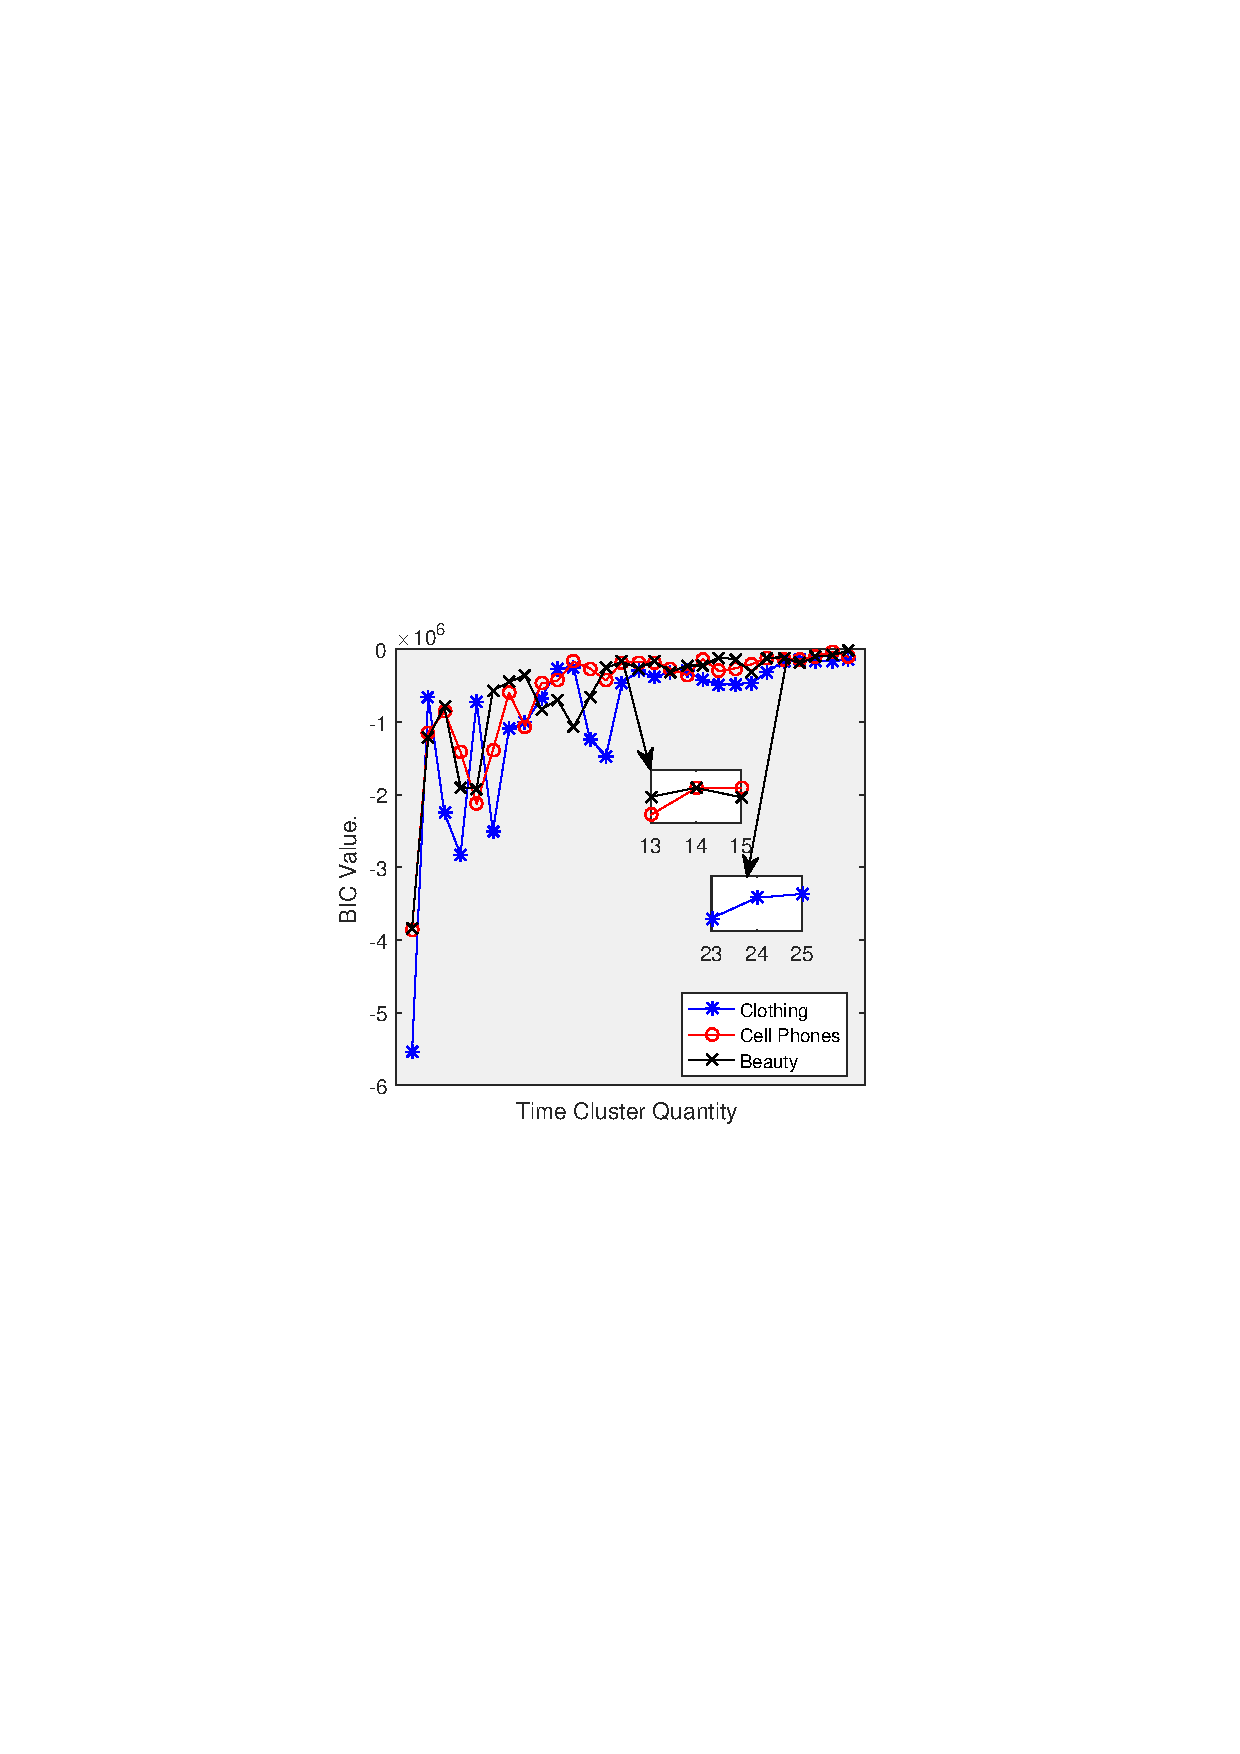
\includegraphics[width=0.43\columnwidth]{chart/bic.pdf}
            \label{bic}
        }
        %
        \subfloat[The number of invalid users.]{
            \centering
            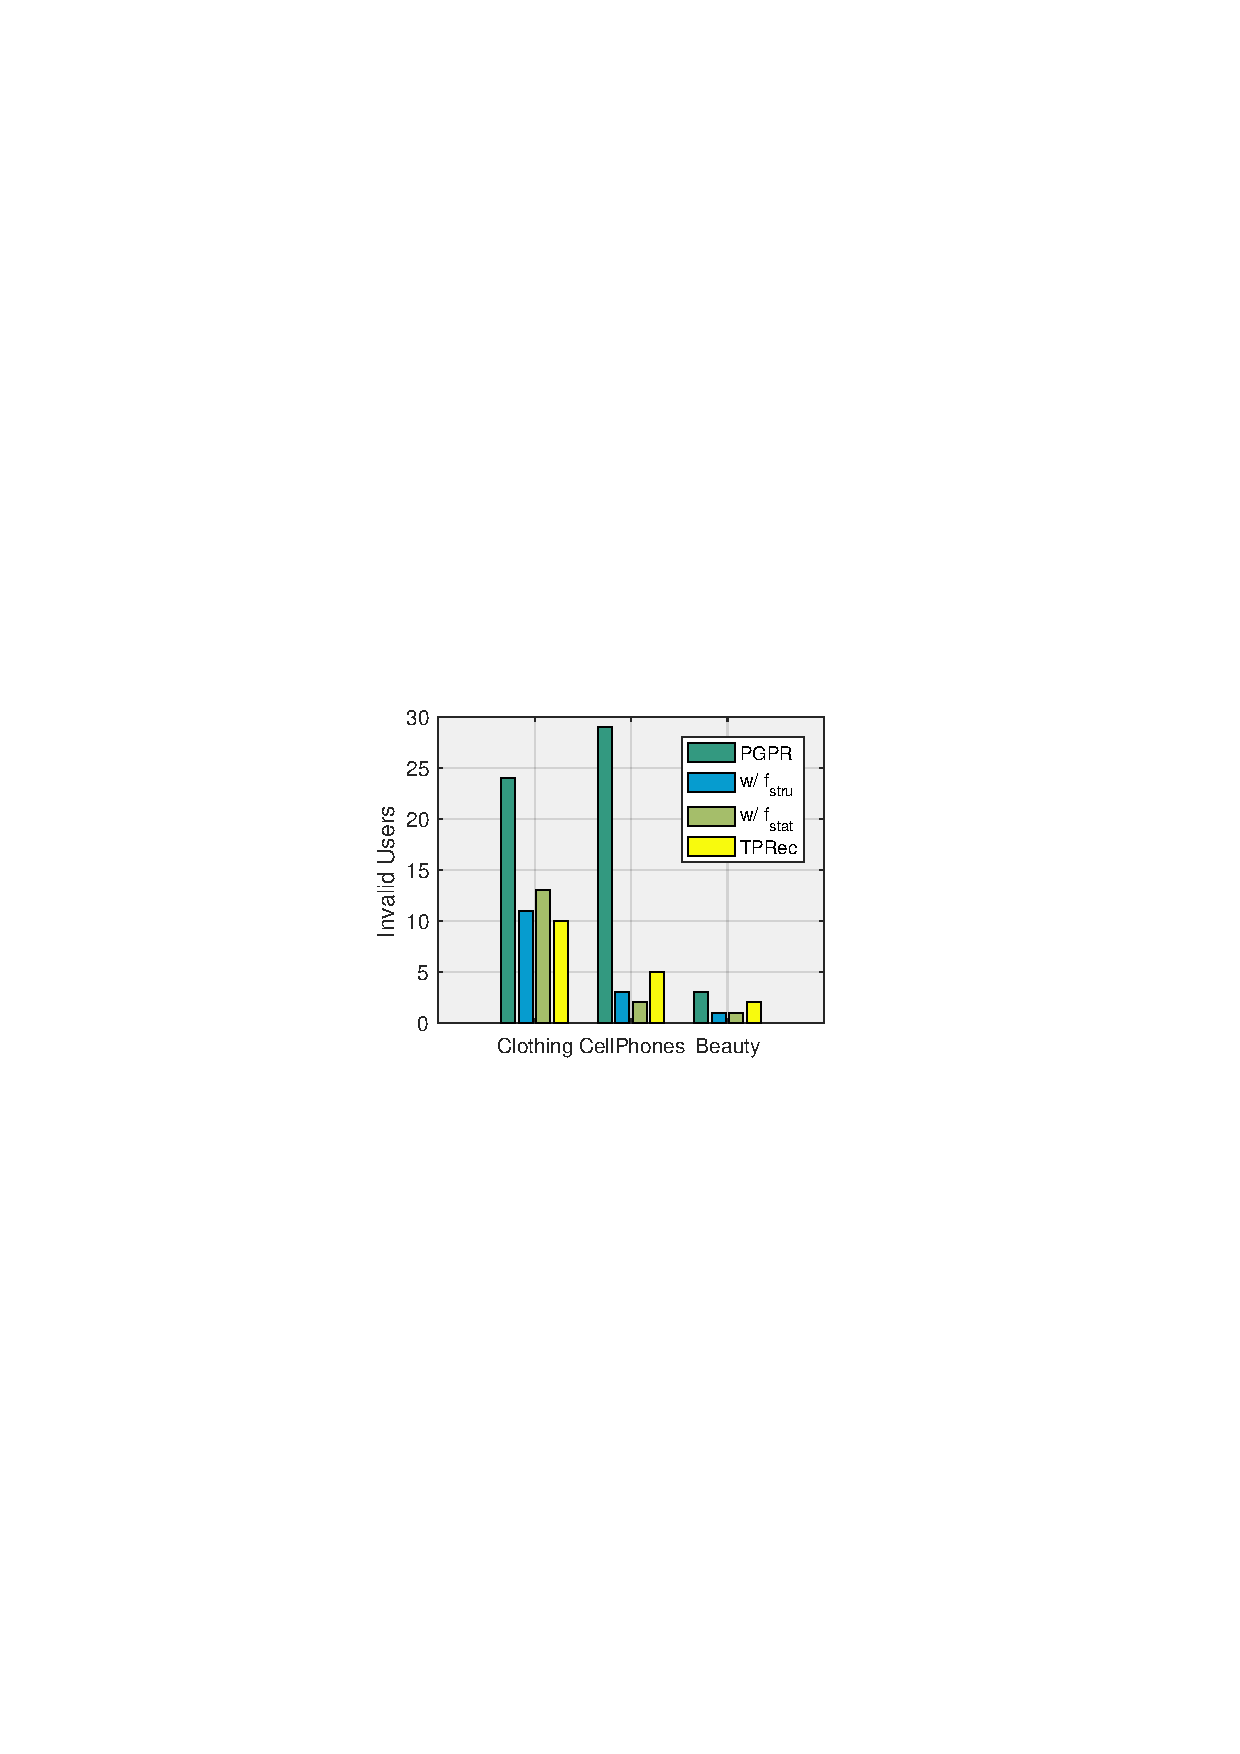
\includegraphics[width=0.5\columnwidth]{chart/invalid_user.pdf}
            \label{invalid}
        }
        %
        \caption{Analyses of different datasets. The left subgraph illustrates how BIC value varies with the clustering number, while the right subgraph illustrates the numbers of invalid users calculated from PGPR and \tkgrec.}
    \end{minipage}
%    \setlength{\abovecaptionskip}{-1pt}
    \vspace{-0.15cm}
\end{figure}

\subsubsection{Implementation Details.}\label{parasetting}
%
%We implement our Markov Decision Process formulation environment, where we
%mainly refer to Xian~\etal~\cite{pgpr} in the implementation.

To reduce the experiment workload and keep the comparison fair, we closely follow the settings of the PGPR work ~\cite{pgpr}.
For the time-aware relation extraction module, we perform relation clustering with GMM and select the optimal number of clusters with Bayesian Information Criterion (BIC) ~\cite{bic}. The BIC value with the clustering number is presented in Figure \ref{bic}. The optimal clustering numbers are 24, 14, and 14 on \textit{Clothing}, \textit{Cell Phones} and \textit{Beauty}, respectively.

For the time-aware representation learning module, we set the embedding size $d$ as $100$, and the dimension $m$ of temporal feature space as $25$, with 16 dimensions for statistical features and 9 dimensions for structural features. More specifically, for statistical features, we 
simply compute the $year(t) \in \mathbb{R}^1$ to be $= current\ year - earliest\ year$, $day(t) \in \mathbb{R}^1 = current\ day - earliest\ day$, $month(t) \in \mathbb{R}^1$ is the month of the year, $week(t) \in \mathbb{R}^8$ is the day in a week and it's one-hot encoding, and $season(t) \in \mathbb{R}^5$ is the season in a year and it's one-hot encoding. For structural features, given a specific timestamp $t_1$, we have $\boldsymbol{f}_{stru}(t_1) \in \mathbb{R}^9$ $= z(t_1)\ ||\ z_{sea}'(t_1)\ ||\ z_{sea}''(t_1)$ $||\ 
\ z_{mon}'(t_1)\ ||\ z_{mon}''(t_1)$ $||\ z_{week}'(t_1)\ ||\ z_{week}''(t_1)
$ $||\ z_{day}'(t_1)\ ||\ z_{day}''(t_1)$.



For the time-aware path reasoning module, we set the maximum episode path length $k$ as $3$ (namely,
the maximum history length is $2$), the default history length $k'$ as 1, and the maximum size of pruned action space as $|\mathcal{A}_k|\leq250$.
Besides, for the parameters in RL, we set the dimension of $x_t$ as 256 and the discount factor $\gamma$ as $0.99$; Also, for the policy/value network, we set $W_1 \in \mathbb{R}^{512 \times
256}$ , $W_a \in \mathbb{R}^{256 \times 251}$ and $W_c \in \mathbb{R}^{256 \times 1}$. We optimize our model for 50 epochs with Adam, where the learning rate is set as 0.0001 and the batch size is 32. During the prediction, we refer to PGPR \cite{pgpr} and set the sampling sizes as $K_1=25$, $K_2=5$, $K_3=1$.

%In our implementation, we adopt a set of parameters for the models' latent
%representation. More specifically, the dimension $m$ of temporal feature space
%is $25$, including $16$-dimensional statistical features and $9$-dimensional
%structural features.
%


%We also adopt a set of parameters for the time-aware path reasoning component.
%%
%Specifically, the maximum episode path length $k$ is set to $3$ (namely,
%the maximum history length is $2$), and the default history length is set to $k'=1$, the maximum size of pruned action space
%is $|\mathcal{A}_u|\leq250$.
%

\subsubsection{Evaluation Metrics.}\label{evalMetric}
%
We adopt four widely used metrics to evaluate recommendation performance including: 
\textit{Normalized Discounted Cumulative Gain@K} (\textit{NDCG@K} for short), 
\textit{Recall@K}, \textit{Precision@K} and \textit{Hit Ratio@K} (\textit{HR@K} for short).
%
The process for obtaining the scores for those metrics is given in Equation (\ref{metric_fun}).

   
% \begin{equation}   \label{metric_fun}
% \begin{split}
% 	 NDCG@K &= \frac{DCG@K}{IDCG@K} &	 Recall@K &= \frac{\left| tp \right|}{\left| tp \right| + \left| fn \right|} \\
% 	 Precision@K &= \frac{\left| tp \right|}{\left| tp \right| + \left| fp \right|} &	 HR@K &=  \frac{N_{hits} @K}{N_{test}}
% 	\end{split}
% \end{equation}
\begin{align}   \label{metric_fun}
	 NDCG@K &= \frac{DCG@K}{IDCG@K} & Recall@K &= \frac{\left| TP \right|}{\left| TP \right| + \left| FN \right|} \notag \\
	 Precision@K &= \frac{\left| TP \right|}{\left| TP \right| + \left| FP \right|} & HR@K &=  \frac{N_{hits} @K}{N_{users}}
\end{align}
Here, \textit{DCG@K} is the  Discounted Cumulative Gain at position K, \textit{IDCG@K} is Ideal Discounted Cumulative Gain through position K, $\left| TP \right|$ means the number of recommended items that are actually relevant at position K, $\left| TP \right| + \left| FN \right|$ is the total number of relevant items and  $\left| TP \right| + \left| FP \right|$ means the number of recommended items at position K. As for \textit{HR@K}, $N_{hits} @K$ is the number of users whose items in the test set at position K, and $N_{users}$ is the total number of users.

%
These metrics reflect how a model retrieves relevant items that users are indeed fond of. A larger score indicates the better performance that a model achieves. In our experiments, we refer to ~\cite{pgpr} and set $\text{K}=10$.



\begin{table}[t!]
\centering
\small
\caption{Normal test performance comparison on three real-world datasets. The results are reported in percentage (\%). The bold font denotes the winner in that column. The row `Impv' indicates the relative performance gain of our \tkgrec~ relative to ADAC.}\label{overallComp}
% \resizebox{\textwidth}{!}{
{
% \begin{tabular}{c|p{0.65cm}<{\centering}ccc|cccc|cccc}
\begin{tabular}{c|p{0.65cm}<{\raggedleft}p{0.65cm}<{\raggedleft}p{0.65cm}<{\raggedleft}p{0.65cm}<{\raggedleft}|
p{0.65cm}<{\raggedleft}p{0.65cm}<{\raggedleft}p{0.65cm}<{\raggedleft}p{0.65cm}<{\raggedleft}|
p{0.65cm}<{\raggedleft}p{0.65cm}<{\raggedleft}p{0.65cm}<{\raggedleft}p{0.65cm}<{\raggedleft}}
\hline  \hline
Models      &
\multicolumn{4}{c|}{\textbf{Clothing}}                               &
\multicolumn{4}{c|}{\textbf{Cell Phones}}                                 &
\multicolumn{4}{c}{\textbf{Beauty}}
\\ \hline
Metrics     & \textbf{NDCG}  & \textbf{Recall} & \textbf{HR}     &
\textbf{Prec.} & \textbf{NDCG}  & \textbf{Recall} & \textbf{HR}    &
\textbf{Prec.} & \textbf{NDCG} & \textbf{Recall} & \textbf{HR}     &
\textbf{Prec.} \\ \hline
BPR         & 0.598          & 1.086           & 1.801          &
0.196              & 1.892          & 3.363           & 5.323           &
0.624              & 2.704         & 4.927           & 9.113           &
1.066              \\
RippleNet   & 0.627          & 1.112           & 1.885          &
0.201              & 1.935          & 3.858           & 5.727           &
0.688              & 2.458         & 5.251           & 9.224           &
1.133              \\
TransRec    & 1.245          & 2.078           & 3.116          &
0.312              & 3.361          & 6.279           & 8.725           &
0.962              & 3.218         & 4.853           & 8.671           &
1.285              \\
PGPR        & 2.871          & 4.827           & 7.023          &
0.723              & 5.042          & 8.416           & 11.904          &
1.274              & 5.573         & 8.476           & 14.682          &
1.744              \\
ADAC        & \underline{3.048}          & \underline{5.027}           & \underline{7.502}          &
\underline{0.763}              & \underline{5.220}           & \underline{8.943}           & \underline{12.537}          &
\underline{1.358}              & \underline{6.080} & \underline{9.424}  & \underline{16.036} &
\underline{1.991}     \\  \hline
%
w/ $\boldsymbol{f_{stru}}$        & 3.074          & 5.132           &
7.484          &
0.778              & \textbf{5.988}          & \textbf{10.185}           &
\textbf{14.278}          & \textbf{1.528}              & \textbf{6.185}
& \textbf{9.582}     & \textbf{16.130}          &
\textbf{2.023}              \\
%
w/ $\boldsymbol{f_{stat}}$        & 2.997          & 5.144           &
7.498          &
0.781              & 5.743          & 9.714           & 13.649          &
1.471              & 5.868         & 9.227           & 15.719          &
1.928              \\
%
\tkgrec\ & \textbf{3.109} & \textbf{5.298}  & \textbf{7.657} &
\textbf{0.798}    &5.643 & 9.572 & 13.553
&1.463     & 5.963 & 9.184 & 15.678 & 1.919              \\   \hline
% \hdashline[0.8pt/3pt] \midrule[0.1mm]
Impv.(\%)    & +2.01          & +5.39           & +2.07          &
+4.59             & +14.71         & +13.89         & +13.89          &
+12.52            & +1.73 & +1.68 & +0.59  & +1.66            \\  \hline  \hline
\end{tabular}
}
\end{table}



% % =========================================
% \begin{table}[t!]
% \centering
% \small
% \caption{Sequence-based performance comparison. The results are reported in percentage (\%). }\label{seqComp}
% % \resizebox{\textwidth}{!}{
% {
% % \begin{tabular}{c|p{0.65cm}<{\centering}ccc|cccc|cccc}
% \begin{tabular}{c|p{0.65cm}<{\raggedleft}p{0.65cm}<{\raggedleft}p{0.65cm}<{\raggedleft}p{0.65cm}<{\raggedleft}|
% p{0.65cm}<{\raggedleft}p{0.65cm}<{\raggedleft}p{0.65cm}<{\raggedleft}p{0.65cm}<{\raggedleft}|
% p{0.65cm}<{\raggedleft}p{0.65cm}<{\raggedleft}p{0.65cm}<{\raggedleft}p{0.65cm}<{\raggedleft}}
% \hline  \hline
% Models      &
% \multicolumn{4}{c|}{\textbf{Clothing}}                               &
% \multicolumn{4}{c|}{\textbf{Cell Phones}}                                 &
% \multicolumn{4}{c}{\textbf{Beauty}}
% \\ \hline
% Metrics     & \textbf{NDCG}  & \textbf{Recall} & \textbf{HR}     &
% \textbf{Prec.} & \textbf{NDCG}  & \textbf{Recall} & \textbf{HR}    &
% \textbf{Prec.} & \textbf{NDCG} & \textbf{Recall} & \textbf{HR}     &
% \textbf{Prec.} \\ \hline
% BERT4Rec	&    0.248 	&    0.516 	&    0.676 	&    0.072 	&    1.612 	&    3.315 	&    4.303 	&    0.456 	&    1.664 	&    3.540 	&    4.552 	&    0.482 \\
% GRU4Rec	&    0.541 	&    1.070 	&    1.391 	&    0.147 	&    3.370 	&    6.365 	&    8.268 	&    0.876 	&    3.813 	&    6.508 	&    8.451 	&    0.896 \\
% NextItNet	&    0.289 	&    0.573 	&    0.741 	&    0.079 	&    2.422 	&    4.683 	&    6.084 	&    0.645 	&    2.360 	&    4.727 	&    6.136 	&    0.650 \\
% SR-GNN	&    0.428 	&    0.797 	&    1.027 	&    0.109 	&    3.072 	&    5.777 	&    7.501 	&    0.795 	&    3.212 	&    5.757 	&    7.416 	&    0.785 \\
% GC-SAN	&    1.116 	&    2.229 	&    2.886 	&    0.306 	&    \underline{4.211} 	&    \underline{8.219} 	&    \underline{10.673} 	&    \underline{1.131} 	&    4.361 	&    7.511 	&    9.763 	&    1.135 \\
% SASRec	&    1.253 	&    2.541 	&    3.302 	&    0.350 	&    3.876 	&    7.695 	&    9.997 	&    1.060 	&    \underline{4.522} 	&    \underline{8.918} 	&    \underline{11.583} 	&    \underline{1.228} \\
% TimelyRec	&    1.263 	&    2.716 	&    3.839 	&    0.395 	&    4.039 	&    7.791 	&    10.212 	&    1.092 	&    \textbf{4.671} 	&    \textbf{9.217} 	&    \textbf{12.723} 	&    \textbf{1.401} \\
% PGPR	&    \underline{2.102} 	&    \underline{3.651} 	&    \underline{5.087} 	&    \underline{0.523} 	&    3.135 	&    4.911 	&    7.820 	&    0.818 	&    3.654 	&    6.060 	&    9.805 	&    1.112 \\ \hline
% w/ $\boldsymbol{f_{stru}}$	&    2.245 	&    3.905 	&    5.447 	&    0.563 	&    4.228 	&    8.936 	&    11.362 	&    1.211 	&    4.331 	&    8.051 	&    10.416 	&    1.138 \\
% w/ $\boldsymbol{f_{stat}}$	&    2.270 	&    3.955 	&    5.518 	&    0.569 	&    4.123 	&    8.767 	&    11.146 	&    1.189 	&    4.175 	&    7.717 	&    10.118 	&    1.131 \\
% \tkgrec\	&    \textbf{2.304} 	&    \textbf{4.027} 	&    \textbf{5.612} 	&    \textbf{0.578} 	&    \textbf{4.292} 	&    \textbf{9.131} 	&    \textbf{11.387} 	&    \textbf{1.216} 	&    4.467 	&    8.773 	&    11.223 	&    1.206 \\
% \hline  \hline
% \end{tabular}
% }
% \end{table}
% % =================


% \begin{table}[t!]
% \caption{Sequence-based performance comparison. The results are reported in percentage (\%). }\label{seqComp}
% \begin{tabular}{c|rr|rr|rr}
% \hline \hline
% \textbf{}    & \multicolumn{2}{c|}{\textbf{Clothing}}           & \multicolumn{2}{c|}{\textbf{Cell Phones}}                                & \multicolumn{2}{c}{\textbf{Beauty}}             \\
% \textbf{Metrics}    & \multicolumn{1}{c}{\textbf{NDCG}} & \multicolumn{1}{c|}{\textbf{Recall}} & \multicolumn{1}{c}{\textbf{NDCG}} & \multicolumn{1}{c|}{\textbf{Recall}} & \multicolumn{1}{c}{\textbf{NDCG}} & \multicolumn{1}{c}{\textbf{Recall}} \\ \hline
% \textbf{BERT4Rec}  & 0.248                             & 0.516                                & 1.612                             & 3.315                                & 1.664                             & 3.540                               \\
% \textbf{GRU4Rec}   & 0.541                             & 1.070                                & 3.370                             & 6.365                                & 3.813                             & 6.508                               \\
% \textbf{NextItNet} & 0.289                             & 0.573                                & 2.422                             & 4.683                                & 2.360                             & 4.727                               \\
% \textbf{SR-GNN}    & 0.428                             & 0.797                                & 3.072                             & 5.777                                & 3.212                             & 5.757                               \\
% \textbf{GC-SAN}    & 1.116                             & 2.229                                & {\underline{4.211}}                       & {\underline{8.219}}                          & 4.361                             & 7.511                               \\
% \textbf{SASRec}    & 1.253                             & 2.541                                & 3.876                             & 7.695                                & {\underline{4.522}}                       & {\underline{8.918}}                         \\
% \textbf{TimelyRec} & 1.263                             & 2.716                                & 4.039                             & 7.791                                & \textbf{4.671}                    & \textbf{9.217}                      \\
% \textbf{PGPR}      & {\underline{2.102}}                       & {\underline{3.651}}                          & 3.135                             & 4.911                                & 3.654                             & 6.060                               \\ \hline
% \textbf{w/ $\boldsymbol{f_{stru}}$}    & 2.245                             & 3.905                                & 4.228                             & 8.936                                & 4.331                             & 8.051                               \\
% \textbf{w/ $\boldsymbol{f_{stat}}$}    & 2.270                             & 3.955                                & 4.123                             & 8.767                                & 4.175                             & 7.717                               \\
% \textbf{\tkgrec}     & \textbf{2.304}                    & \textbf{4.027}                       & \textbf{4.292}                    & \textbf{9.131}                       & 4.467                             & 8.773                               \\ \hline \hline
% \end{tabular}
% \end{table}

\begin{table}[t!]
\caption{Sequence-based performance comparison. The results are reported in percentage (\%). }\label{seqComp}
\begin{tabular}{c|cc|rr|rr|rr}
\hline \hline
\multirow{2}{*}{\textbf{Models}} & \multicolumn{2}{c|}{\textbf{Side Infomation}} & \multicolumn{2}{c|}{\textbf{Clothing}}                                   & \multicolumn{2}{c|}{\textbf{Cell Phones}}                                & \multicolumn{2}{c}{\textbf{Beauty}}                                     \\ \cline{2-9} 
                         & \multicolumn{1}{c}{\textbf{KG?}}       & \multicolumn{1}{c|}{\textbf{Time?}}      & \multicolumn{1}{c}{\textbf{NDCG}} & \multicolumn{1}{c|}{\textbf{Recall}} & \multicolumn{1}{c}{\textbf{NDCG}} & \multicolumn{1}{c|}{\textbf{Recall}} & \multicolumn{1}{c}{\textbf{NDCG}} & \multicolumn{1}{c}{\textbf{Recall}} \\ \hline
BERT4Rec  &   $\times$                 &          \checkmark                & 0.248                             & 0.516                                & 1.612                             & 3.315                                & 1.664                             & 3.540                               \\
GRU4Rec  &   $\times$                 &          \checkmark                         & 0.541                             & 1.070                                & 3.370                             & 6.365                                & 3.813                             & 6.508                               \\
NextItNet &   $\times$                 &          \checkmark                         & 0.289                             & 0.573                                & 2.422                             & 4.683                                & 2.360                             & 4.727                               \\
SR-GNN   &   $\times$                 &          \checkmark                          & 0.428                             & 0.797                                & 3.072                             & 5.777                                & 3.212                             & 5.757                               \\
GC-SAN    &   $\times$                 &          \checkmark                         & 1.116                             & 2.229                                & \underline{4.211}                       & \underline{8.219}                          & 4.361                             & 7.511                               \\
SASRec  &   $\times$                 &          \checkmark                         & 1.253                             & 2.541                                & 3.876                             & 7.695                                & \underline{4.522}                       & \underline{8.918}                         \\
TimelyRec &   $\times$                 &          \checkmark                         & 1.263                             & 2.716                                & 4.039                             & 7.791                                & \textbf{4.671}                    & \textbf{9.217}                      \\
PGPR      &     \checkmark               &      $\times$                    & \underline{2.102}                       & \underline{3.651}                          & 3.135                             & 4.911                                & 3.654                             & 6.060                               \\ \hline
w/ $\boldsymbol{f_{stru}}$      &     \checkmark               &       \checkmark                   & 2.245                             & 3.905                                & 4.228                             & 8.936                                & 4.331                             & 8.051                               \\
w/ $\boldsymbol{f_{stat}}$       &     \checkmark               &       \checkmark                        & 2.270                             & 3.955                                & 4.123                             & 8.767                                & 4.175                             & 7.717                               \\
\tkgrec     &     \checkmark               &       \checkmark                         & \textbf{2.304}                    & \textbf{4.027}                       & \textbf{4.292}                    & \textbf{9.131}                       & 4.467                             & 8.773                               \\ \hline \hline
\end{tabular}
\end{table}

\subsection{Performance Comparison (RQ1)}
\label{rq1}
%精确度, 以及那个啥, invalid users(介绍invalid的时候提一嘴原因放在RQ3讲).
Table \ref{overallComp} presents the performance of the compared normal test methods in terms of four evaluation metrics.  For the sake of
clarity, the row `Impv' shows the relative improvement achieved by our \tkgrec\ or w/ $\boldsymbol{f_{stru}}$ over the best baselines. 
Table \ref{seqComp} presents the sequence-based recommendation methods performance comparison.
The boldface font denotes the winner in that column.
We make the following observations:

\subsubsection{\textbf{\tkgrec~ Vs. existing normal test methods.}}
From Table \ref{overallComp}, we observe our \tkgrec~ always achieve the best performance among all compared methods. Especially in the dataset Cell Phones, the improvement of w/ $\boldsymbol{f_{stru}}$ over best baselines are quite impressive --- 14.71\%, 13.89\%, 13.89\%, and 12.52\% in terms of NDCG, Recall, HR, and Precision, respectively. 
%
% And our \tkgrec~ significantly better (p=0.0015 \textless 0.05) than those open source baselines (PGPR, TransRec, \textit{etc}.) with three repeated trials. 
%
And our \tkgrec~ performs significantly better ($p$-value \textless\ 0.05) than those open source baselines (PGPR, TransRec, \textit{etc}.) with three repeated trials.
%
This result validates that by leveraging temporal information our \tkgrec~ is able to find higher-quality reasoning paths.  

We make a further investigation to provide more insights. We refer to a path as an \textit{invalid path} if the path starts from a user but doesn't end at an item entity within three hops (note that we set the path length $k=3$). We also refer to a target user that we predict  as an \textit{invalid user} if he has less than 10 \textit{valid} paths. As shown in Figure \ref{invalid}, we find the number of \textit{Invalid Users} in \tkgrec\ is consistently less than PGPR which does not consider temporal information. This result suggests that time-aware rewards adopted by \tkgrec\ indeed guide the RL agent towards exploration better.


%Firstly, \tkgrec\ consistently yields the best performance on Clothing and Cell
%Phones datasets. In particular, \tkgrec\ improves over the SOTA path-reasoning
%baseline PGPR {\it w.r.t.} NDCG by  7.49\%, 11.92\%,7.01\% and {\it w.r.t.} HR
%by 8.49\%, 13.85\%, 6.78\% in Amazon Clothing, Cell Phones and Beauty,
%respectively. Note that these evaluation results are obtained for the top-10
%predicted items for every user in the test set.
%However, \tkgrec\ is slightly worse than ADAC on the Beauty dataset because of
%adaptability of the different mechanisms. The details will be discussed later.
%
%\footnote{\hxie{Should explain a little bit on why \tkgrec\ performs worse on
%Beauty compared against ADAC.}}

%We make further investigations into the above results.
%%
%We refer to a path as an \textit{invalid path} if the path starts from a user
%but doesn't end at an item entity within three hops (note that we set the path
%length $k=3$).
%%
%We also refer to a user as an \textit{invalid user} if the user we predict has
%less than 10 \textit{valid} paths.
%%
%As shown in Figure \ref{invalid}, we find the number of \textit{Invalid Users}
%in \tkgrec\ is consistently less than in PGPR.
%%
%This suggests that out
%time-aware based reward adopted in \tkgrec\ can guide the RL agent to explore better.
%
%We further make the following observations.
%%
%Firstly, \tkgrec\ consistently yields the best performance on Clothing and Cell
%Phones datasets. In particular, \tkgrec\ improves over the SOTA path-reasoning
%baseline PGPR {\it w.r.t.} NDCG by  7.49\%, 11.92\%,7.01\% and {\it w.r.t.} HR
%by 8.49\%, 13.85\%, 6.78\% in Amazon Clothing, Cell Phones and Beauty,
%respectively. Note that these evaluation results are obtained for the top-10
%predicted items for every user in the test set.
%%
%This verifies the validity of the temporal side information in recommendation.
% And jointly analyzing Figure[cite]

%\begin{figure}[htbp]
%%\centerline{
\includegraphics{fig1.png}}
%
\includegraphics[width=0.47\textwidth]{invalid_cmp.pdf}
%\caption{Results of each dataset's invalid users number.}
%\label{invalid_cmp}
%\end{figure}
\subsubsection{\textbf{Comparison in terms of different datasets.}}
 Interestingly, in normal test setting, we observe that the improvement of our \tkgrec\ over recent work on the datasets Clothing and Cell Phones are relatively large, while relatively small on the dataset Beauty. This result can be explained by the difficulty of different datasets. From Figure \ref{invalid}, we observe that the number of invalid users on the Beauty dataset generated by PGPR is $3$, while the number increases to $24$ and $29$ on other datasets. This result validates that path reasoning on Beauty is relatively easier than on other datasets. PGPR or ADAC also achieve pretty good performance on Beauty. Correspondingly, our \tkgrec\ does not obtain much gain on Beauty.

\subsubsection{\textbf{Reasoning Vs. Unreasoning.}}
 We also observe that KG-based reasoning methods (\ie, PGPR, ADAC and \tkgrec) outperform other KG-based methods (\ie, RippleNet) on all three datasets across all four evaluation metrics. This result clearly validates the superiority of conducting path reasoning on knowledge graph. Though reasoning, interpretability is not against accuracy. It not only increases interpretability, but also boosts model accuracy.
 
 \subsubsection{\textbf{\tkgrec~ Vs. existing sequence-based  methods.}}
 From Table \ref{seqComp}, we can see the performance of \tkgrec\ and PGPR is lower than that at normal test setting.
%  and our \tkgrec\ achieve the best performance on the \textit{Clothing} and the \textit{Cell Phones} datasets, whereas, slightly worse than TimelyRec and SASRec on the \textit{Beauty} dataset.
% From Table \ref{seqComp}, we can see our \tkgrec\ achieve the best performance on the \textit{Clothing} and the \textit{Cell Phones} datasets, whereas, slightly worse than TimelyRec and SASRec on the \textit{Beauty} dataset.
%  the performance of our \tkgrec\ and PGPR is lower than that at normal test setting,
One possible reason of the performance drop is the Out-of-Distribution (OOD) setting in the sequence-based experiment, which means the test distribution is different from the training.
% That performance degradation is because the sequence-based experimental setting mentioned in Section \ref{dataset} is Out-of-Distribution(OOD), which means the testing distribution is different from the training. 
%
Our \tkgrec\ achieves the best performance on the \textit{Clothing} and the \textit{Cell Phones} datasets, whereas, slightly worse than TimelyRec and SASRec on the \textit{Beauty} dataset.
It is appropriate to emphasize that these sequential recommendation methods are specifically designed for predicting the next item that the user would interact, which sacrifices explainability. Our \tkgrec\ can not only provide explanations about why an item is suitable for a user, but also achieve comparable recommendation accuracy in sequential recommendation.
% Since our sequence-based experimental setting mentioned in Section \ref{dataset} is Out-of-Distribution(OOD), 
% we can see the performance of our \tkgrec\ is slightly worse than TimelyRec and SASRec on the \textit{Beauty} dataset, but achieve the best performance on the \textit{Clothing} and the \textit{Cell Phones} datasets. 


We further make the following observations. In the \textit{Clothing} dataset, even PGPR is much better than other sequence-based methods, which indicates that the KG side information is really useful in the \textit{Clothing} dataset. Additionally, our \tkgrec\ consistently beats PGPR in all  datasets, and \tkgrec\ performs better than the other two versions, $w/ f_{stru}$ and $w/ f_{stat}$. 
%
Notably, there is 10\% of the interactions in validation set between training set and test set in sequence-based comparison, and the time-series clustering method doesn't know the interaction distribution around the test set, which is different from normal test setting. 
Hence, $w/ f_{stru}$'s effect is not enough to support such experiments, it needs to be supplemented by $w/ f_{stat}$.
%
% 其中, 由于在seq实验设置下, 训练集和测试集之间存在验证集的间隔, 并且聚类方法完全没有见过测试集附近的商品购买分布分布, 这和正常设置下不同.
%因此wstru的效果不足以支撑这样的实验, 需要wstat进行补充.
%
This verifies the validity of our time-aware reasoning methodology.

%Secondly, by compare the performance of ADAC and \tkgrec\ in Table
%\ref{overallComp}, and analyze the results in Figure \ref{invalid}, we observe
%that the number of invalid users on the Beauty dataset generated by PGPR is
%$3$; however, this number increases dramatically to $25$ and $29$ on the
%Clothing and Cell Phones dataset, respectively.
%%
%This means that it is easier to perform recommendation tasks on the Beauty
%dataset than on the other two datasets,
%%least ten times less than the other two.
%suggesting that the temporal information available in the Beauty dataset has
%less contribution to improve the overall performance.
%%
%Additionally, ADAC adopts the Shortest Path (SP) as its expert
%demonstration~\cite{ADAC}
%to achieve adversarial learning,
%%
%%\footnote{\hxie{what do you mean by ``expert demonstration''?}}
%%
%which is intuitively simpler and more straightforward, but more suitable for
%Beauty dataset.
%%
%Thus, our \tkgrec\ performs slightly worse than ADAC in Beauty dataset, but
%still better than other baseline models.
%%
%What's more, \tkgrec's invalid users number in Clothing dataset is larger than
%the other two datasets and it does not decrease much compared to
%PGPR. This is consistent with the Imp(\%) performance of Clothing is not as
%good as the Cell Phones dataset.





%%====================================================================
%%消融实验, 以PGPR为基准, 加时间轴, 再加deep metric learning, 再加RNN,
%%再加time-aware %reasoning(原来的PGPR就采用, purchase平均值一把梭).
%To explore the effect of temporal information, we compare results of
%our
%\tkgrec\
%model on different modalities over the Amazon Cell Phones
%dataset. \textbf{PGPR} is a classic KG reasoning recommendation model
%and we
%set it as the baseline. \textbf{\tkgrec+t} replaces CKG in PGPR with TKG
%and uses
%TransE method to get entities/relations representation,
%while \textbf{\tkgrec+te} uses TKGE method(Section \ref{TKGE}) to encode
%the
%temporal KG.
%\textbf{\tkgrec+tr} adds personalized time-aware reward to w/o te.
%And \textbf{TGRec+trl}, which is the full picture of our \tkgrec, uses
%bidirectional LSTM to encode the state vector compares with \tkgrec+tr.
%The performance comparison results are presented in
%Table \ref{abCmpt} and Figure \ref{abCmp}. We have the following
%observations:
%% 刚加时间轴的时候, 精确度是立马下降的.
%\begin{itemize}
%\item As expected, the method that includes all modules outperforms the
%baseline (PGPR), as shown in Table \ref{abCmpt}.
%
%\item The TKG plays an important role in our method, but added it
%directly to
%the baseline caused a sharp decline (at least -67.63\%) in two metrics.
%Even
%added the TKGE method only improved a little. The reason for this may
%be that
%the multiple time modes interfered the path reasoning phase, and made
%the
%policy network learned wrong pattern. To verify this statement, the
%method
%\textbf{TGRec + tr} with personalized time-aware reward significantly
%improved
%the values of prec. and rec., as shown in Figure \ref{abCmp}.
%
%\item The BiLSTM encoder module is designed to capture implicit
%dependencies
%between hops. However, its effect on beauty dataset is worse than
%ordinary FC
%network in TGRec + tr. As mentioned in \textbf{(RQ1)}, the beauty
%dataset is
%simpler than other datassets, which means our method may cause overfit
%on
%simple dataset.
%\end{itemize}
%%====================================================================

\begin{table}[t!]
\caption{Characteristics and performance of \tkgrec\ and its variants in normal test setting.  The `Imp(\%).' is relative to \tkgrec.}\label{abCmpt}
\resizebox{\textwidth}{27mm}{
\begin{tabular}{c|cc|cc|llllll}
% \begin{tabular}{c|cc|cc|p{0.7cm} p{0.7cm} p{0.7cm} p{0.7cm} p{0.7cm} p{0.7cm}}
\hline \hline
\multirow{3}{*}{Methods} & \multicolumn{2}{c|}{Reasoning With.}                                                    & \multicolumn{2}{c|}{Equipped with.}                                            & \multicolumn{6}{c}{Performance}                                                                                  \\ \cline{2-11} 
                         & Time-aware                                 & BLSTM                                      & Statistical                                & Structural                                 & \multicolumn{2}{c|}{Clothing}            & \multicolumn{2}{c|}{Cell Phones}         & \multicolumn{2}{c}{Beauty} \\ \cline{6-11} 
                         & Reward?                                    & Encoder?                                   & Feature?                                   & Feature?                                   & Prec.    & \multicolumn{1}{l|}{Recall}   & Prec.    & \multicolumn{1}{l|}{Recall}   & Prec.        & Recall      \\ \hline
\textbf{PGPR}            & \multirow{2}{*}{$\times$}    & \multirow{2}{*}{$\times$}    & \multirow{2}{*}{$\times$}    & \multirow{2}{*}{$\times$}    & 0.723    & \multicolumn{1}{l|}{4.827}    & 1.274    & \multicolumn{1}{l|}{8.416}    & 1.744        & 8.476       \\
Imp(\%)                  &                                            &                                            &                                            &                                            & -9.40  & \multicolumn{1}{l|}{-8.89}  & -12.9 & \multicolumn{1}{l|}{-12.1} & -9.12      & -7.71     \\ \hline
\textbf{w/o R}         & \multirow{2}{*}{$\times$}    & \multirow{2}{*}{\checkmark} & \multirow{2}{*}{\checkmark} & \multirow{2}{*}{\checkmark} & 0.191    & \multicolumn{1}{l|}{1.374}    & 0.317    & \multicolumn{1}{l|}{1.909}    & 0.712        & 3.031       \\
Imp(\%)                  &                                            &                                            &                                            &                                            & -76.1 & \multicolumn{1}{l|}{-74.1} & -78.3 & \multicolumn{1}{l|}{-80.1} & -62.9     & -67.0    \\ \hline
\textbf{w/o L}         & \multirow{2}{*}{\checkmark} & \multirow{2}{*}{$\times$}    & \multirow{2}{*}{\checkmark} & \multirow{2}{*}{\checkmark} & 0.786    & \multicolumn{1}{l|}{5.205}    & 1.450    & \multicolumn{1}{l|}{9.534}    & 1.927        & 9.200       \\
Imp(\%)                  &                                            &                                            &                                            &                                            & -1.50  & \multicolumn{1}{l|}{-1.76}  & -0.89  & \multicolumn{1}{l|}{-0.40}  & +0.42       & +0.17      \\ \hline
\textbf{w/ $\boldsymbol{f_{stru}}$}     & \multirow{2}{*}{\checkmark} & \multirow{2}{*}{\checkmark} & \multirow{2}{*}{$\times$}    & \multirow{2}{*}{\checkmark} & 0.778    & \multicolumn{1}{l|}{5.132}    & 1.528    & \multicolumn{1}{l|}{10.185}   & 2.023        & 9.582       \\
Imp(\%)                  &                                            &                                            &                                            &                                            & -2.51  & \multicolumn{1}{l|}{-3.13}  & +4.44   & \multicolumn{1}{l|}{+6.40}   & +5.42       & +4.33      \\ \hline
\textbf{w/ $\boldsymbol{f_{stat}}$}     & \multirow{2}{*}{\checkmark} & \multirow{2}{*}{\checkmark} & \multirow{2}{*}{\checkmark} & \multirow{2}{*}{$\times$}    & 0.781    & \multicolumn{1}{l|}{5.144}    & 1.471    & \multicolumn{1}{l|}{9.714}    & 1.928        & 9.227       \\
Imp(\%)                  &                                            &                                            &                                            &                                            & -2.13  & \multicolumn{1}{l|}{-2.91}  & +0.55   & \multicolumn{1}{l|}{+1.48}   & +0.47       & +0.47      \\ \hline
\textbf{\tkgrec}      & \checkmark                  & \checkmark                  & \checkmark                  & \checkmark                  & 0.798    & \multicolumn{1}{l|}{5.298}    & 1.463    & \multicolumn{1}{l|}{9.572}    & 1.919        & 9.184       \\ \hline \hline
\end{tabular}}
\end{table}




% \begin{figure}[]
% 	\centering
% 	\subfloat[Clothing.]{
% 		\begin{minipage}[t]{0.3\textwidth}
% 			\centering
% 			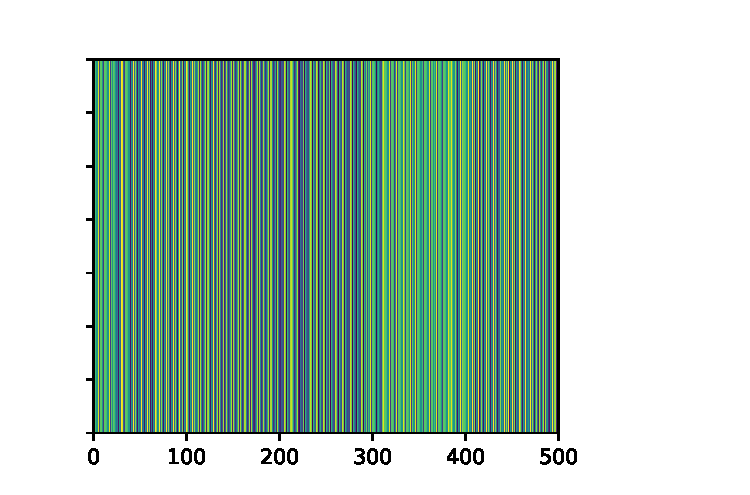
\includegraphics[width=1\textwidth]{chart/clothNone.pdf}
% 		\end{minipage}
% 	}
% 	\subfloat[Clothing-$\boldsymbol{f_{stat}}$]{
% 		\begin{minipage}[t]{0.3\textwidth}
% 			\centering
% 			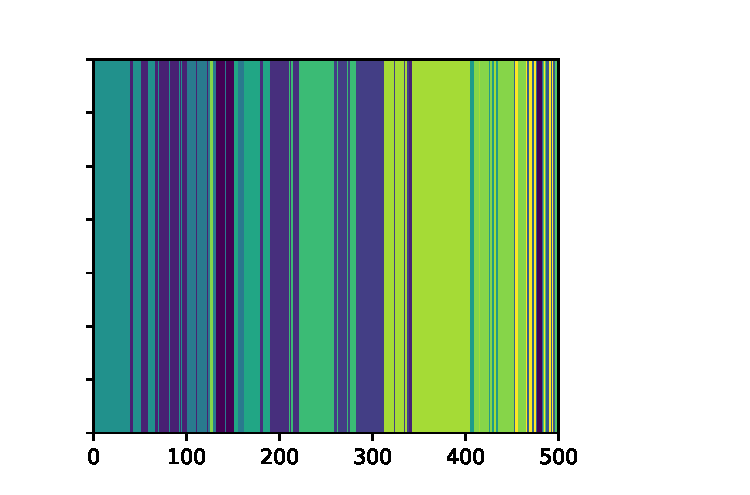
\includegraphics[width=1\textwidth]{chart/clothminus_stat.pdf}
% 		\end{minipage}
% 	}
% 	\subfloat[Clothing-$\boldsymbol{f_{stru}}$]{
% 		\begin{minipage}[t]{0.345\textwidth}
% 			\centering
% 			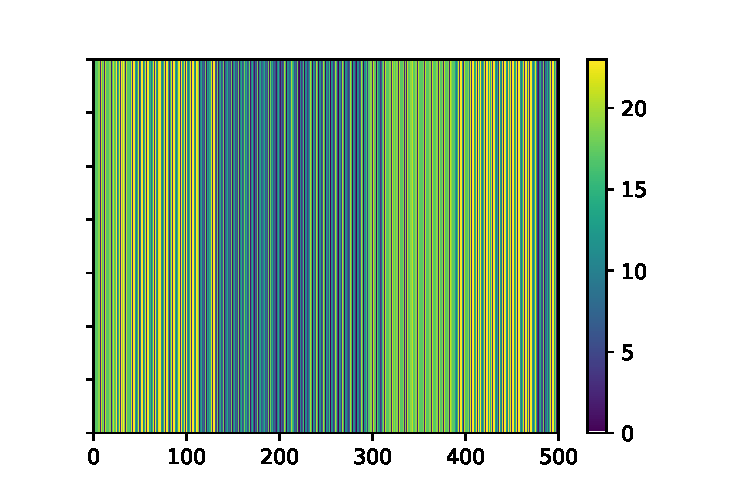
\includegraphics[width=1\textwidth]{chart/clothminus_stru.pdf}
% 		\end{minipage}
% 	}
	
% 	\subfloat[Cell Phones.]{
% 		\begin{minipage}[t]{0.3\textwidth}
% 			\centering
% 			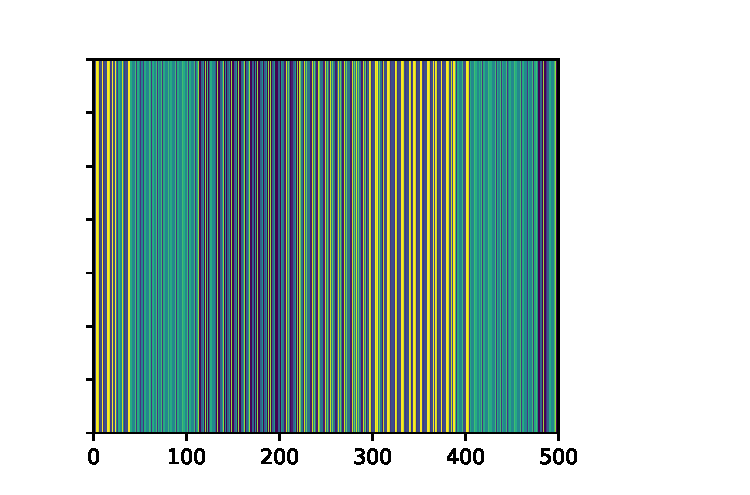
\includegraphics[width=1\textwidth]{chart/cellNone.pdf}
% 		\end{minipage}
% 	}
% 	\subfloat[Cell Phones-$\boldsymbol{f_{stat}}$]{
% 		\begin{minipage}[t]{0.3\textwidth}
% 			\centering
% 			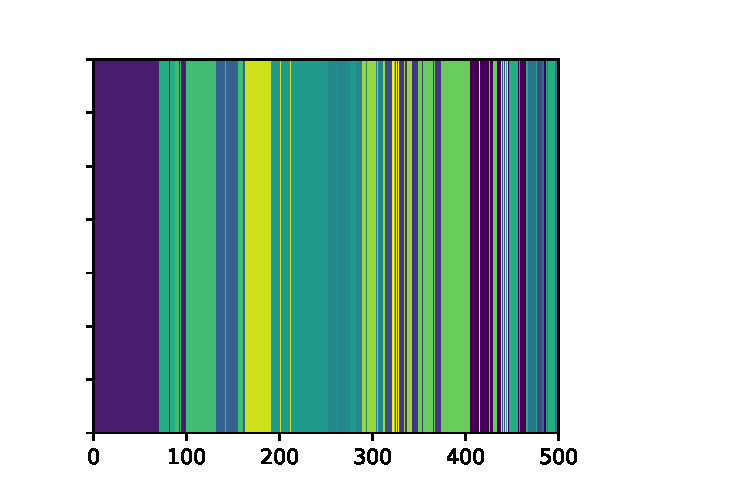
\includegraphics[width=1\textwidth]{chart/cellminus_stat.pdf}
% 		\end{minipage}
% 	}
% 	\subfloat[Cell Phones-$\boldsymbol{f_{stru}}$]{
% 		\begin{minipage}[t]{0.345\textwidth}
% 			\centering
% 			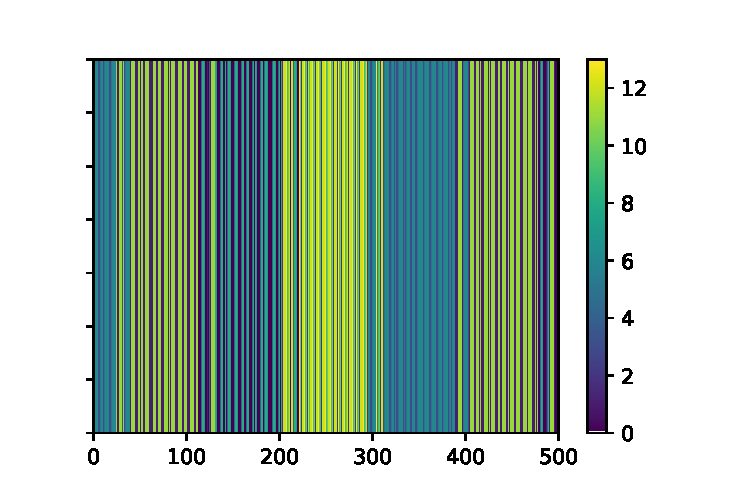
\includegraphics[width=1\textwidth]{chart/cellminus_stru.pdf}
% 		\end{minipage}
% 	}
	
% 	\subfloat[Beauty.]{
% 		\begin{minipage}[t]{0.3\textwidth}
% 			\centering
% 			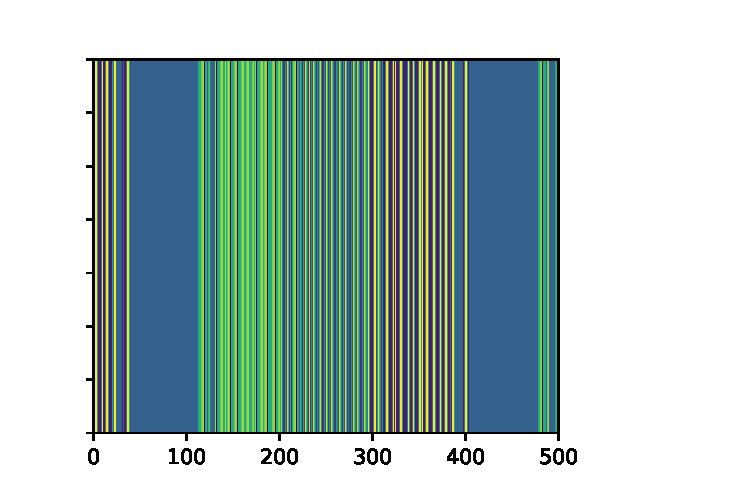
\includegraphics[width=1\textwidth]{chart/beautyNone.pdf}
% 		\end{minipage}
% 	}
% 	\subfloat[Beauty-$\boldsymbol{f_{stat}}$]{
% 		\begin{minipage}[t]{0.3\textwidth}
% 			\centering
% 			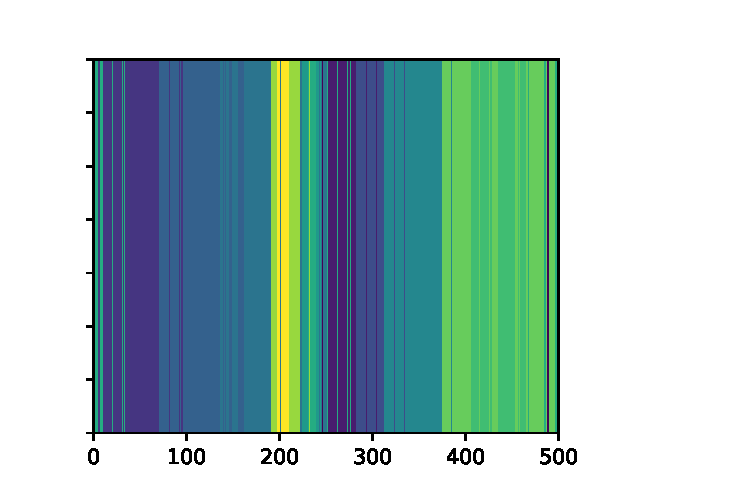
\includegraphics[width=1\textwidth]{chart/beautyminus_stat.pdf}
% 		\end{minipage}
% 	}
% 	\subfloat[Beauty-$\boldsymbol{f_{stru}}$]{
% 		\begin{minipage}[t]{0.345\textwidth}
% 			\centering
% 			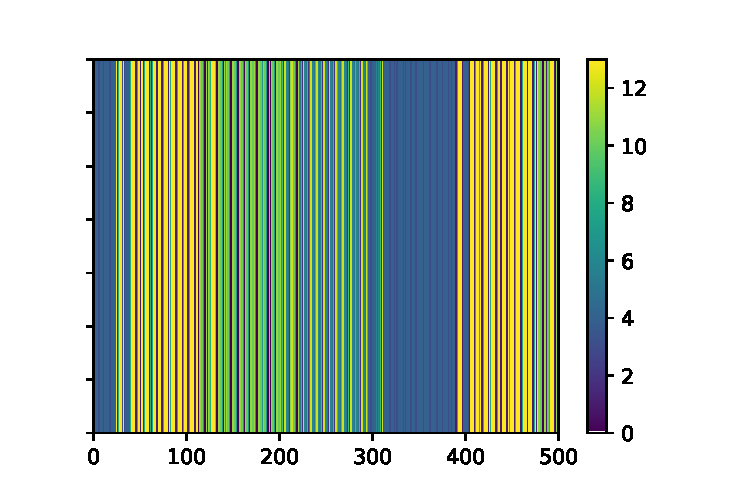
\includegraphics[width=1\textwidth]{chart/beautyminus_stru.pdf}
% 		\end{minipage}
% 	}
% \caption{Visualization of the clustering of the relations with varying timestamp.
% The color represents the class that the timestamp belongs to. 
% }
% 	\label{cluster}
% \end{figure}

\begin{figure}[tb]
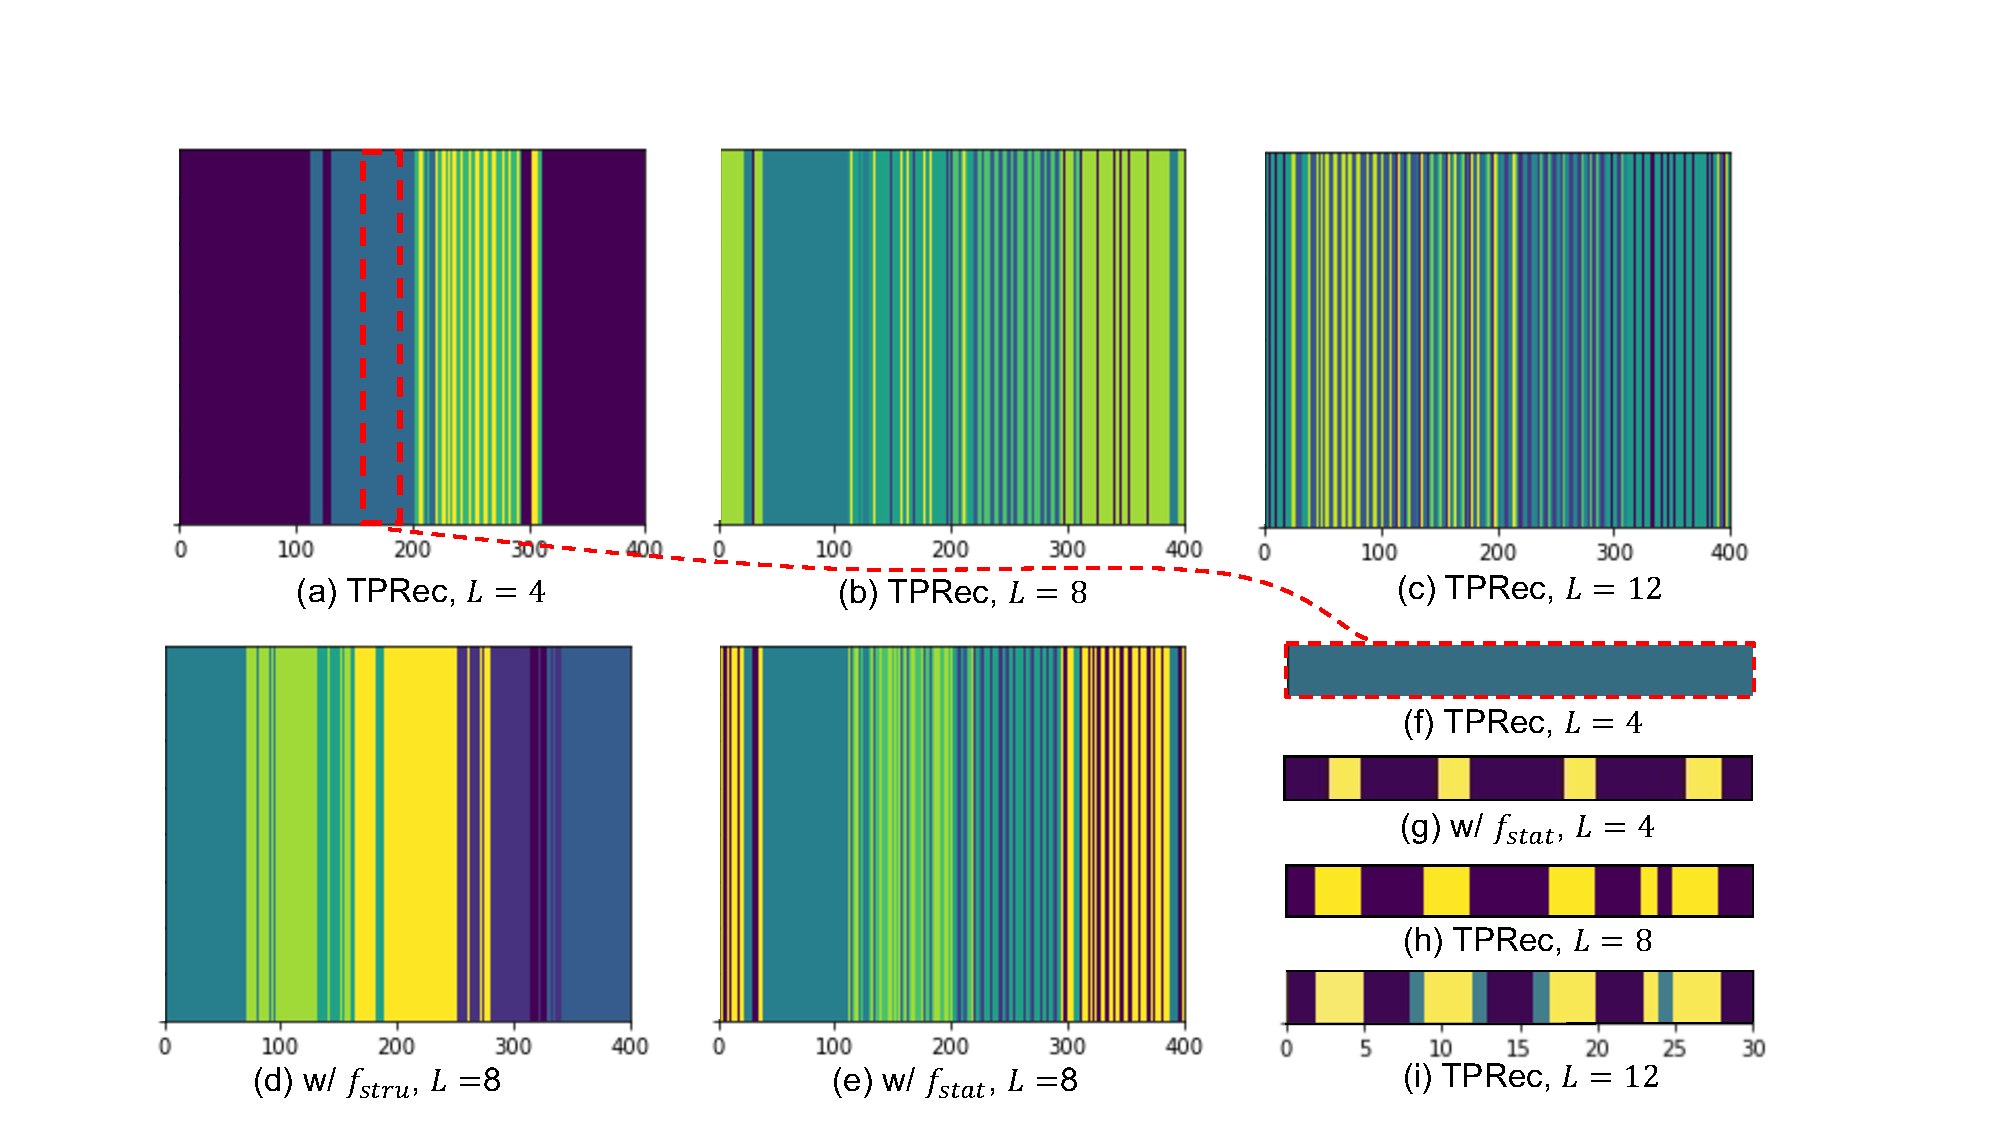
\includegraphics[width=\columnwidth]{chart/cluster_colorbar3.pdf}
\caption{ Visualization of the clustering of the relations with varying timestamp on the \textit{Cell Phones} dataset. 
The color represents the class that the timestamp belongs to. 
				}
		\label{cluster}
\end{figure}


\subsection{Ablation Study (RQ2)}

Note that \tkgrec\ improves PGPR mainly in the following three aspects: using temporal features to extract relations, adopting personalized time-aware reward strategy, and using bidirectional LSTM to encode the state vector. To show the impact of these aspects, besides making a comparison among three versions of \tkgrec\ (w/ $\boldsymbol{f_{stru}}$, w/ $\boldsymbol{f_{stat}}$ and \tkgrec ), we further conduct ablation studies and compare \tkgrec\ with its two variants: (1) \textit{w/o R} that removes personalized time-aware weighting strategy $W_{h_u}$ in generating rewards and uses average pooling instead. (2) \textit{w/o L} that replaces bidirectional LSTM with a simple fully connected layer as PGPR.  The characteristics and performance of these methods are presented in Table \ref{abCmpt}.

\subsubsection{\textbf{Effectiveness of using temporal features.}}
 First, we observe our \tkgrec  (\ie, w/ $\boldsymbol{f_{stru}}$, w/ $\boldsymbol{f_{stat}}$ and \tkgrec) that use temporal features consistently outperform PGPR. This result validates the essence of temporal information in making recommendation. We then make a comparison among three versions of \tkgrec. To our surprising, w/ $\boldsymbol{f_{stru}}$ that just uses structure features usually achieves better performance than \tkgrec\ 
which uses both statistical and structural features in normal test setting. To gain more insights of this phenomenon, we visualize the results of the \textit{Cell Phones} dataset  clustering in Figure \ref{cluster}, and the other two datasets have similar performance.
 %
 We observe that with the cluster number $L$ gaining, the clustering result in \tkgrec\ turns to be more complicated. 
 %
%  For example, in Figure \ref{cluster}a, the \tkgrec\ clustering result is similar with the four seasons in a year, and then we focus on 30 days in the second season (Figure \ref{cluster}f). As the $L$ grew to $8$, it broke the seasons pattern, and capable to obtain weekend-like clusters (Figure \ref{cluster}h). It's worth noting that w/ $\boldsymbol{f_{stat}}$ (Figure \ref{cluster}g) also distinguishes between weekdays and weekends, but our \tkgrec\ clustering is more flexible, which 
% is benefit from the structural features.
%  When $L = 12$, in Figure \ref{cluster}c and \ref{cluster}i, the clusters become even more precisely.  
 %
 For example, in Figure \ref{cluster}a, the clustering result of \tkgrec\ is similar with the four seasons in one year,
and then we focus on 30 days in the second season (Figure \ref{cluster}f). As the $L$ grew to $8$, it broke the seasons' pattern, and could obtain weekend-like clusters (Figure \ref{cluster}h). It’s worth noting that w/ $\boldsymbol{f_{stat}}$ (Figure \ref{cluster}g) also distinguishes between weekdays and weekends, but our \tkgrec\ clustering is more flexible, which benefits from the structural features. When $L = 12$ in Figures \ref{cluster}c and \ref{cluster}i, the clusters become even more precise. 
%
 Furthermore, in Figure \ref{cluster}b, \ref{cluster}d and \ref{cluster}e, 
 we can see that the clustering is more stable in w/ $\boldsymbol{f_{stru}}$, where the interactions with similar tendencies are more likely to be clustered into the same class, while we observe relatively heavy fluctuation in w/ $\boldsymbol{f_{stat}}$. 
 %
%  Additionally, Figure \ref{cluster}f-i shows the clustering result in a shorter and clearer manner.
 %
 This interesting phenomenon suggests that the structural features deduced from user behaviors provide an important and reliable signal in capturing interaction similarity, while statistical features exhibit weak or even noisy correlation with the similarity. Nonetheless, the statistical features sometimes are also useful and serve as a complement for relation extraction. It can be seen from the better performance of \tkgrec\ over w/ $\boldsymbol{f_{stru}}$ on dataset Clothing and all three datasets in sequence-based test setting.

\subsubsection{\textbf{Effectiveness of using time-aware reward.}}
From Table \ref{abCmpt}, when removing personalized time-aware weighting strategy in reward, we observe significant performance degradation (higher than 69.21\%) of w/o R compared with \tkgrec. w/o R even performs worse than PGPR. This interesting phenomenon clearly reveals the importance of using personalized weights. Time-aware relations are indeed useful for path reasoning, but they require to be carefully exploited. Only if we finely differentiate the contribution of each type of relation, can we sufficiently enjoy the merits of such information.





%When  ignoring the user's personalized history and directly adopting a fixed
%interaction relation as reasoning reward,  it
%leads to a significant performance degradation of at least -69.21\%
%on all datasets. The reason is that

\subsubsection{\textbf{Effectiveness of using bidirectional LSTM}}
By comparing w/o L with \tkgrec, generally speaking, we can conclude that using bidirectional LSTM could boost recommendation performance. This result can be attributed to the powerful capacity of BLSTM in capturing dependency between reasoning hops.  However, on the dataset Beauty, \tkgrec\ performs closely or even worse than w/o L. This phenomenon can be attributed to the specialty of Beauty. As discussed in Section~\ref{rq1}, Beauty is a relatively simple dataset and does not need such complex structure. The advanced BLSTM may not bring much gain on Beauty and instead would increase the risk of over-fitting.




%Last but not least, \tkgrec\ uses bidirectional LSTM to encode the
%state vector,
%compared against \textbf{w/o L}.
%%
%The BLSTM encoder module is designed to capture implicit dependencies between
%hops and indeed works. However, its effect on beauty dataset is worse than the
%ordinary FC network in w/o L  (see Table \ref{abCmpt}).
%%
%As mentioned in Section~\ref{rq1}, the beauty dataset is simpler than other
%datasets, which means our \tkgrec\ method may be too complicated on Beauty
%dataset, thus leads to performance degradation.



%in and continuous when remove $\boldsymbol{f_{stat}}$, and fluctuate more
%severely when remove $\boldsymbol{f_{stru}}$
%
%Firstly, \textbf{w/o $\boldsymbol{f_{stat}}$} and
%\textbf{w/o $\boldsymbol{f_{stru}}$}
%are the variants with the corresponding temporal feature removed. The
%statistical feature is proposed to measure some time rules like seasonal
%or week changes. The structural feature is proposed to capture users'
%shopping behaviors.
%%
%Figure \ref{cluster} is the visualization of time clustering result derived from Figure
%\ref{day_cmp}.  Figure \ref{cluster} shows that the clustering result is more
%stable and continuous when remove $\boldsymbol{f_{stat}}$, and fluctuate more
%severely when remove $\boldsymbol{f_{stru}}$. \tkgrec\ make a compromise between the above two.
%%
%Specifically, the performance of w/o $\boldsymbol{f_{stat}}$ in Beauty
%dataset outperforms ADAC, while $\boldsymbol{f_{stru}}$ performs worse than ADAC, even compared to \tkgrec. It demonstrates that stability and continuity are more effective on Beauty dataset.
%%
%The comparison between w/o $\boldsymbol{f_{stat}}$,
%w/o $\boldsymbol{f_{stat}}$ and \tkgrec\ in Table \ref{overallComp} and
%Table \ref{abCmpt} shows that
%%stru的效果一直都比stat好, 说明它更重要.
%%而适当地结合这两者能够在特定的数据集上取得更好的结果(cloth).
%%而不管是哪种特征, 聚类结果都比没有引入时间聚类的PGPR更好,
%%说明time-aware确实更有效.
%the effect of w/o $\boldsymbol{f_{stat}}$ consistently better than
%w/o $\boldsymbol{f_{stru}}$, indicating that $\boldsymbol{f_{stru}}$
%is more important in our model.
%And combining those two features can achieve better results on some datasets
%(\eg, Clothing.).
%
%What's more, those time-aware reasoning methods (\ie,
%w/o $\boldsymbol{f_{stat}}$,
%w/o $\boldsymbol{f_{stat}}$ and \tkgrec) outperform normal KG reasoning
%method (\ie, PGPR), which confirms the effectiveness of the time-aware method.

%






%\tkgrec\ has multiple key components in its design. These components include the
%use of the temporal features, the
%use of temporal information to shape a personalized time-aware reward, and the
%use of the bidirectional LSTM to encode the state vector.
%
%In order to evaluate the effect of each component in \tkgrec, we
%start with \tkgrec (note that it includes all components designed to optimize
%for the
%best results), separately remove certain components to generate several
%variants, and compare the results on the three datasets.
%%
%We summarize the variants as follows:
%%
%\begin{itemize}
%%
%%\item \textbf{w/o ErL} is the variant with the least number of components.
%%    It replaces original knowledge graphs with the TKG we proposed, learns the
%%        entities/relations representation by using only the TransE method and
%%        shape the reward by selecting a fixed interaction relation, and encodes
%%        the state vector with a simple FC layer in policy network, which is the
%%        same in PGPR.
%%%
%%\item \textbf{w/o rL} is the variant with the temporal knowledge graph and
%%    TKGE method only. Compared against w/o ErL, it additionally uses the
%%        TKGE method (as described in Section~\ref{trl}) to encode the
%%        temporal KG, aiming to increase the semantics and temporal in the
%%        representation.
%%%
%%\item \textbf{w/o L} uses temporal information to shape a personalized
%%    time-aware reward, which serves as a guide signal in KG reasoning.
%%
%%
%\item \textbf{w/o $\boldsymbol{f_{stat}}$} removes the statistical features
%from temporal feature space $\mathcal{T}$. It extracts the time-aware
%interaction relation by using only the structural features.
%%
%\item \textbf{w/o $\boldsymbol{f_{stru}}$} removes the structural features
%from temporal feature space $\mathcal{T}$.
%%%
%%\item \textbf{w/o E} removes the time-aware representation learning
%%component from \tkgrec.
%%It learns the entities/relations representation by using only the TransE
%%method.
%%
%\item \textbf{w/o R} removes the personalized time-aware reward from
%\tkgrec. The reward is shaped by selecting a fixed interaction relation as in
%the PGPR approach.
%%
%\item \textbf{w/o L} is the variant removes the bidirectional LSTM and
%encodes the state vector with a simple FC layer in policy network, which is the
%        same in PGPR.
%%
%\end{itemize}







%
%
%Firstly, \textbf{w/o E} is the variant which replaces original
%knowledge graphs in PGPR with the time-aware interaction relations we
%proposed,
%and uses TransE method to
%get entities/relations representation.
%%
%As mentioned in Section \ref{tire}, time-aware interaction plays an important
%role in our method.
%%
%%However, when directly using TCKG instead of KG, it leads to a significant
%%performance degradation of at least -67.63\% on all datasets.
%%
%The reason is that the multiple time modes interfered the path reasoning phase,
%thus makes the policy network learn the wrong pattern.
%% TRL 造成了效果的下降, 虽然下降, 但是下降趋势并不明显, 因此重要度没有很大.
%
%
%Secondly, \textbf{w/o R}
%% 对应下面那一段, 下降幅度剧增, 说明很重要, 是key.
%uses the TKGE method to encode the temporal KG.
%The comparison between w/o rL and w/o ErL
%shows that when using w/o rL (namely, adding TKGE to w/o ErL), the
%performance improves by 0.64 \textasciitilde 10.21(\%)  on w/o ErL, but is
%far from making up for the loss caused by TKG.
%%show that \tkgrec+tE can
%%increase the
%%effect of 0.64~10.21(\%) on \tkgrec+t, but still cannot make up for the
%%loss caused by TKG.
%That means the TKGE method can indeed improve
%recommendation, but is still not able to achieve the desired performance.
%
%% 对应加上下面那一段结合使用.
%Thirdly, \textbf{w/o L} is designed to solve the poor performance
%caused by TKG, which uses temporal information to assist in
%reasoning with personalized time-aware reward.
%%
%Figure \ref{abCmp} shows that with the help of the temporal information, its
%performance rises
%rapidly once the personalized time-aware reward is added.
%
%% 这一段结合上一段, 这一段就写stat喝stru的作用吧, 同时mention一下那个图.
%Last but not least, \textbf{\tkgrec}\ uses bidirectional LSTM to encode the
%state vector,
%compared against w/o L.
%%
%The BLSTM encoder module is designed to capture implicit dependencies between
%hops and indeed works. However, its effect on beauty dataset is worse than the
%ordinary FC network in w/o L  (see Figure \ref{beautyCMp}).
%%
%As mentioned in Section~\ref{rq1}, the beauty dataset is simpler than other
%datasets, which means our \tkgrec\ method may be too complicated on Beauty
%dataset, thus leads to performance degradation.


% \begin{table}[t!]
% \caption{Characteristics and performance of \tkgrec~full and its variants.  The `\%Improv.' is relative to
% w/o full.}\label{abCmpt}
% \begin{tabular}{|c|cc|cc|cc|}
% % \toprule
% \hline
% Dataset              & \multicolumn{2}{c|}{\textbf{Clothing}} &
% \multicolumn{2}{c|}{\textbf{Cell Phones}} & \multicolumn{2}{c|}{\textbf{Beauty}}
% \\ \hline
% Metrics(\%)          & Precision              & Recall              &
% Precision               & Recall                & Precision             & Recall
% \\ \hline
% \textbf{PGPR} & 0.723              & 4.827             &
% 1.274               & 8.416               & 1.744             & 8.476
% \\ \hline
% \textbf{\tkgrec}  & 0.798              & 5.298             &
% 1.463               & 9.572               & 1.919             & 9.184
% %\\
% %\%Improv.            & \textbf{+10.37}    & \textbf{+9.76}    &
% %\textbf{+14.84}     & \textbf{+13.74}     & +10.03\%          &
% %+8.35\%
% \\ \hline
% \textbf{w/o $\boldsymbol{f_{stat}}$}   & 0.778 & 5.132 & 1.528 & 10.185 &
% 2.023 &
% 9.582
% \\
% \%Improv.            & -2.77 & -3.44 & +5.10 & +7.28 & +5.96 & +4.69
% \\ \hline
% \textbf{w/o $\boldsymbol{f_{stru}}$}  & 0.781 & 5.144 & 1.471 & 9.714 &
% 1.928 &
% 9.227
% \\
% \%Improv.          & -2.35 & -3.19 & +0.63 & +1.69 & +0.52 & +0.51
% \\ \hline
% \textbf{w/o R} & 0.191 & 1.374 & 0.317 & 1.909 & 0.712 & 3.031
% \\
% \%Improv.           & -83.96 & -81.29 & -89.95 & -91.05 & -69.21 &
% -72.59
% \\ \hline
% \textbf{w/o L}  & 0.786 & 5.205 & 1.450 & 9.534 & 1.927 & 9.200
% \\
% \%Improv.           & -1.66 & -1.93 & -1.02 & -0.45 & +0.46 & +0.19
% % \\ \bottomrule
% \\ \hline
% \end{tabular}
% \end{table}
% Please add the following required packages to your document preamble:
% \usepackage{multirow}
% Please add the following required packages to your document preamble:
% \usepackage{multirow}


%\begin{figure}[]
%	\centering
%	\subfloat[Clothing.]{
%		\begin{minipage}[t]{0.15\textwidth}
%			\centering
%			
\includegraphics[width=1\textwidth]{cloth_cmp.pdf}
%		\end{minipage}
%	}
%	\subfloat[Cell Phones.]{
%		\begin{minipage}[t]{0.15\textwidth}
%			\centering
%			
\includegraphics[width=1\textwidth]{cell_cmp.pdf}
%		\end{minipage}
%	}
%	\subfloat[Beauty.]{
%		\begin{minipage}[t]{0.15\textwidth}
%			\centering
%			
\includegraphics[width=1\textwidth]{beauty_cmp.pdf}\label{beautyCMp}
%		\end{minipage}
%	}
%\caption{Effect tendency of modalities.  From left-to-right
%are Base, TKGRec-ErL, TKGRec=rL, TKGRec-L, TKGRec.}
%	\label{abCmp}
%\end{figure}



\begin{figure}[]
	\centering
	\subfloat[Clothing.]{
		\begin{minipage}[t]{0.33\textwidth}
			\centering
			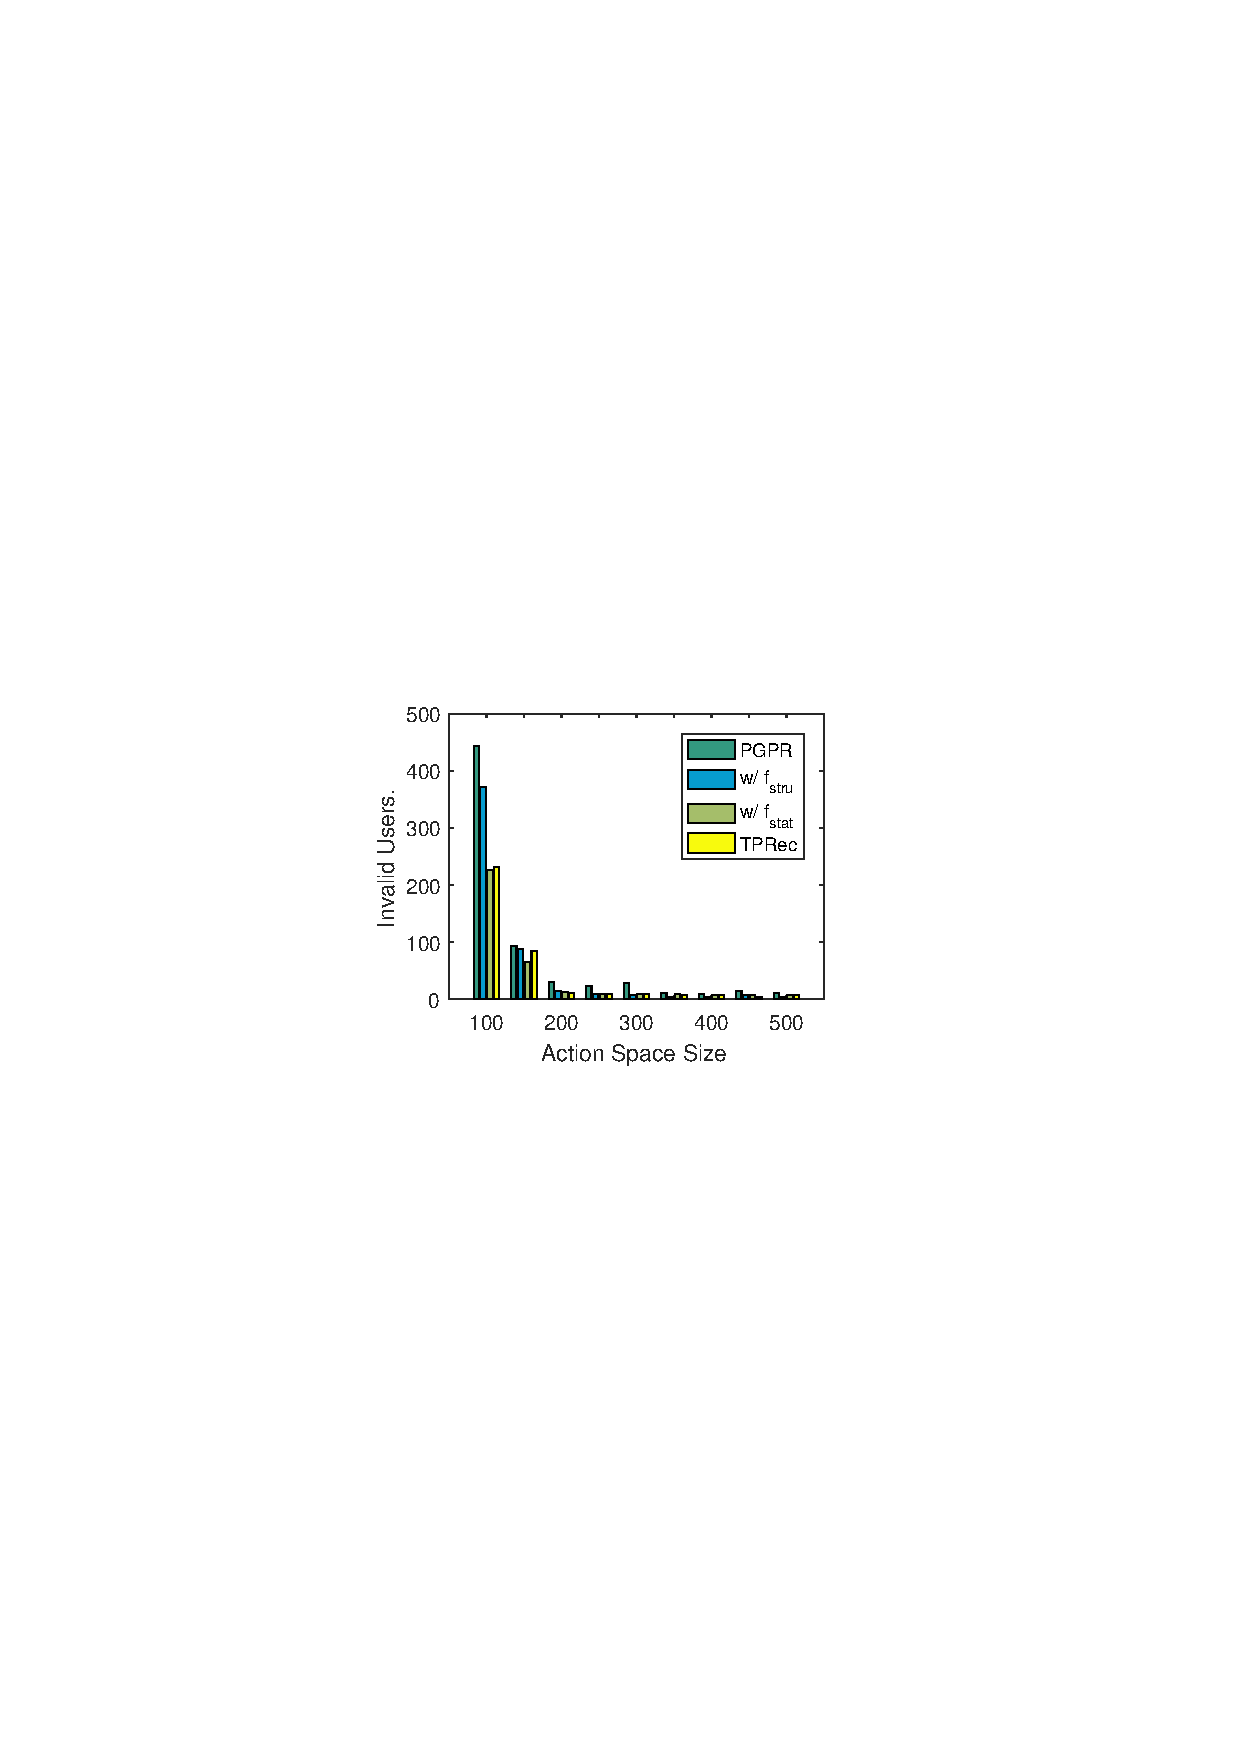
\includegraphics[width=1\textwidth]{chart/cloth_invalid_act.pdf}
		\end{minipage}
	}
	\subfloat[Cell Phone.]{
		\begin{minipage}[t]{0.33\textwidth}
			\centering
			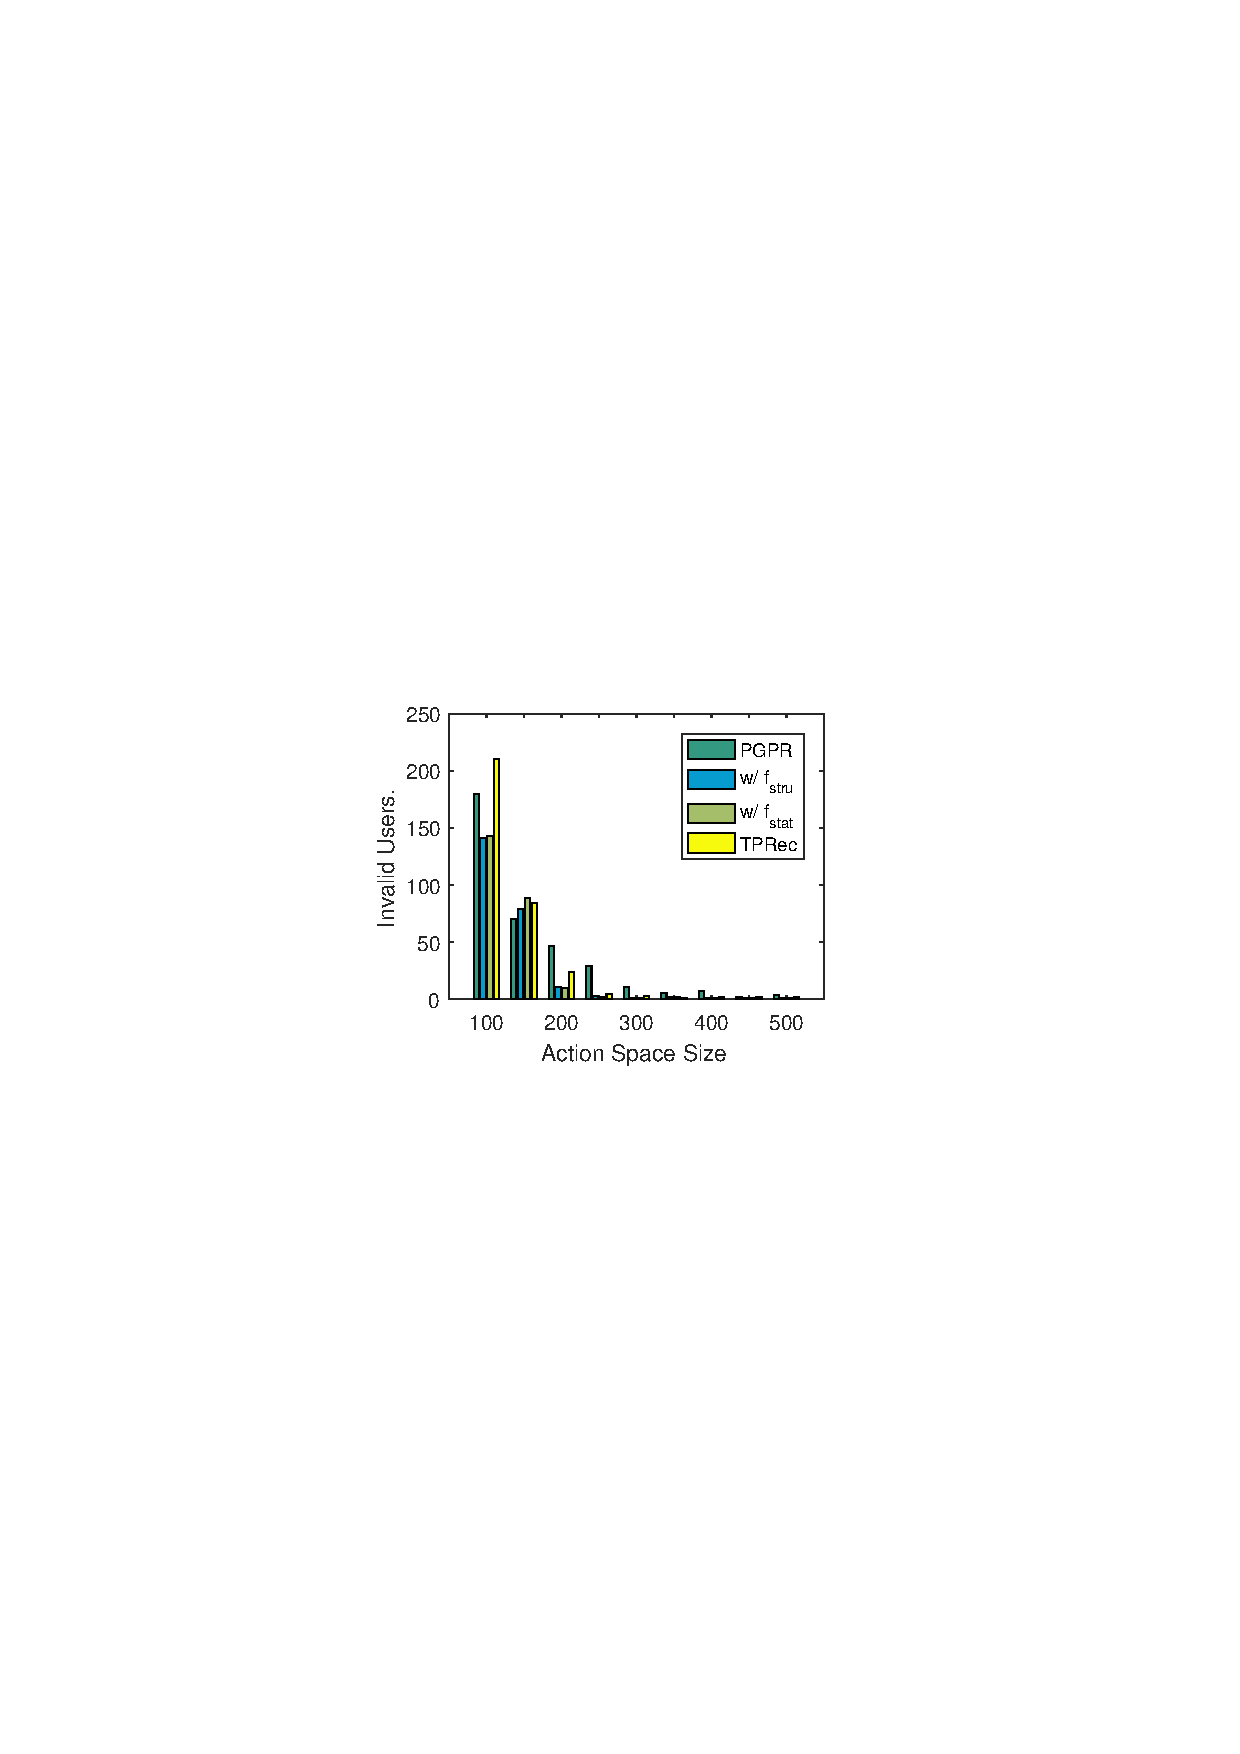
\includegraphics[width=1\textwidth]{chart/cell_invalid_act.pdf}
		\end{minipage}
	}
	\subfloat[Beauty.]{
		\begin{minipage}[t]{0.33\textwidth}
			\centering
			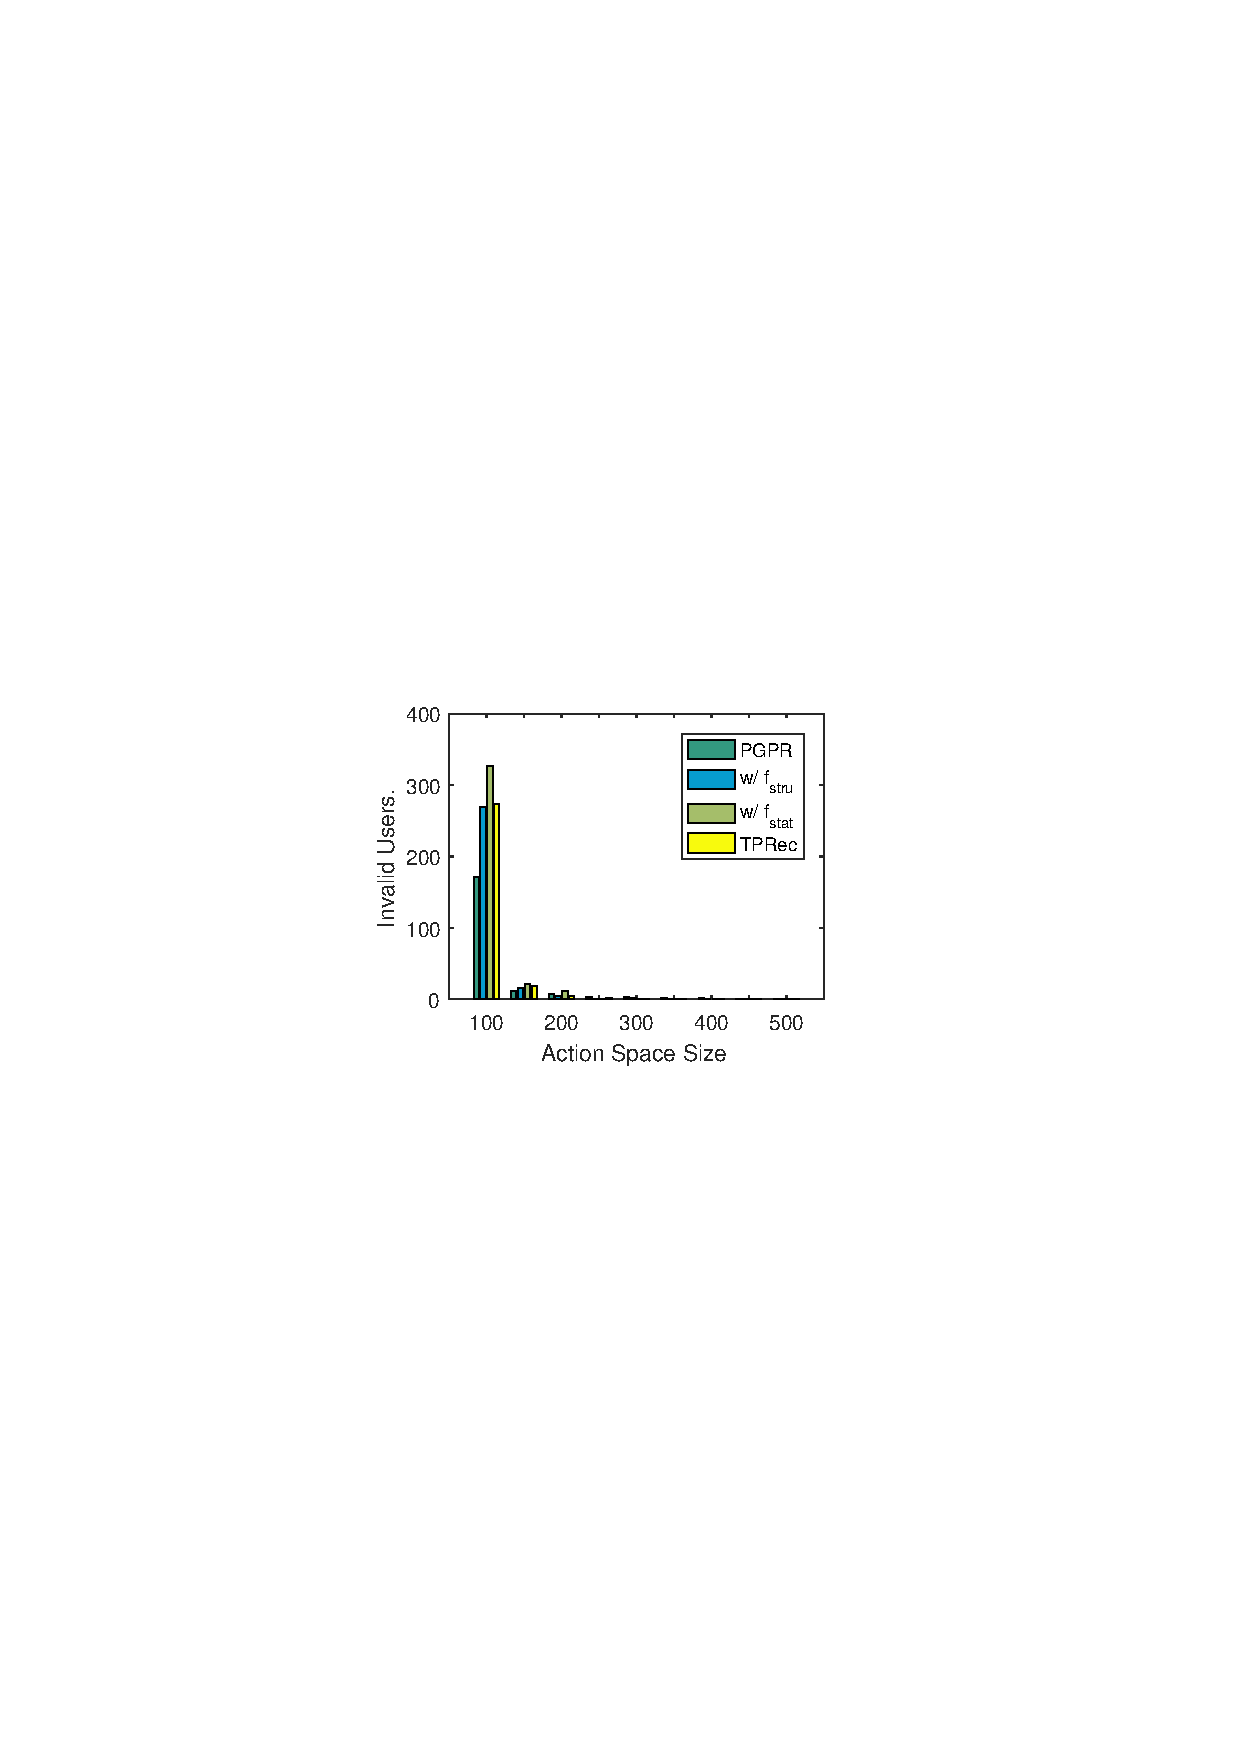
\includegraphics[width=1\textwidth]{chart/beauty_invalid_act.pdf}
		\end{minipage}
	}
\caption{ Invalid User number of varying action space size $\epsilon$.
}
	\label{act_invalid}
\end{figure}

\subsection{Parameter Study on Path Reasoning Module. (RQ3)}
To provide more insights on the time-aware path reasoning module, we test the performance of \tkgrec\ with different time cluster quantity, action space size $\epsilon$ and state history length $k'$.

\subsubsection{\textbf{Effect of Time Cluster Quantity.}}
Figure \ref{cluster_num} presents the performance of four compared methods with different time 
cluster $L$ in range \{4, 8, 12, 16, 20, 24 \}. We make the following three observations: (1) With few exceptions, our \tkgrec\ consistently outperforms PGPR in all three datasets. 
(2) In the Cell Phones and Beauty dataset, all three versions of \tkgrec\ perform better when the number of time cluster $L = 12$ or $16$. And when $L$ is too small or too large, the performance of all three methods drops slightly.  
(3) In the Cloth dataset, when $L$ increases, the performance of our methods is relatively stable.
% This demonstrates the validity of our strategy to adaptively determine time cluster number by BIC value, which is mentioned in Section \ref{parasetting}. 
This is consistent with our strategy to adaptively determine time cluster number by BIC value (in Section \ref{parasetting}), and shows that BIC value can provide a suitable reference for clustering number $L$. 
% and show that BIC can provide a good reference for clustering number.
% It demonstrates we could set time clusters $L$ with reference to BIC value, instead of naive searching for $L$.
% When L increases, the accuracy of our method does not drop too much.
%
% -- The performance in Cloth dataset is insensitive to $L$, that could because the temporal information is not so useful than KG information in Cloth dataset. 
%
\begin{figure}[]
	\centering
	\subfloat[NDCG (Clothing).]{
		\begin{minipage}[t]{0.25\textwidth}
			\centering
			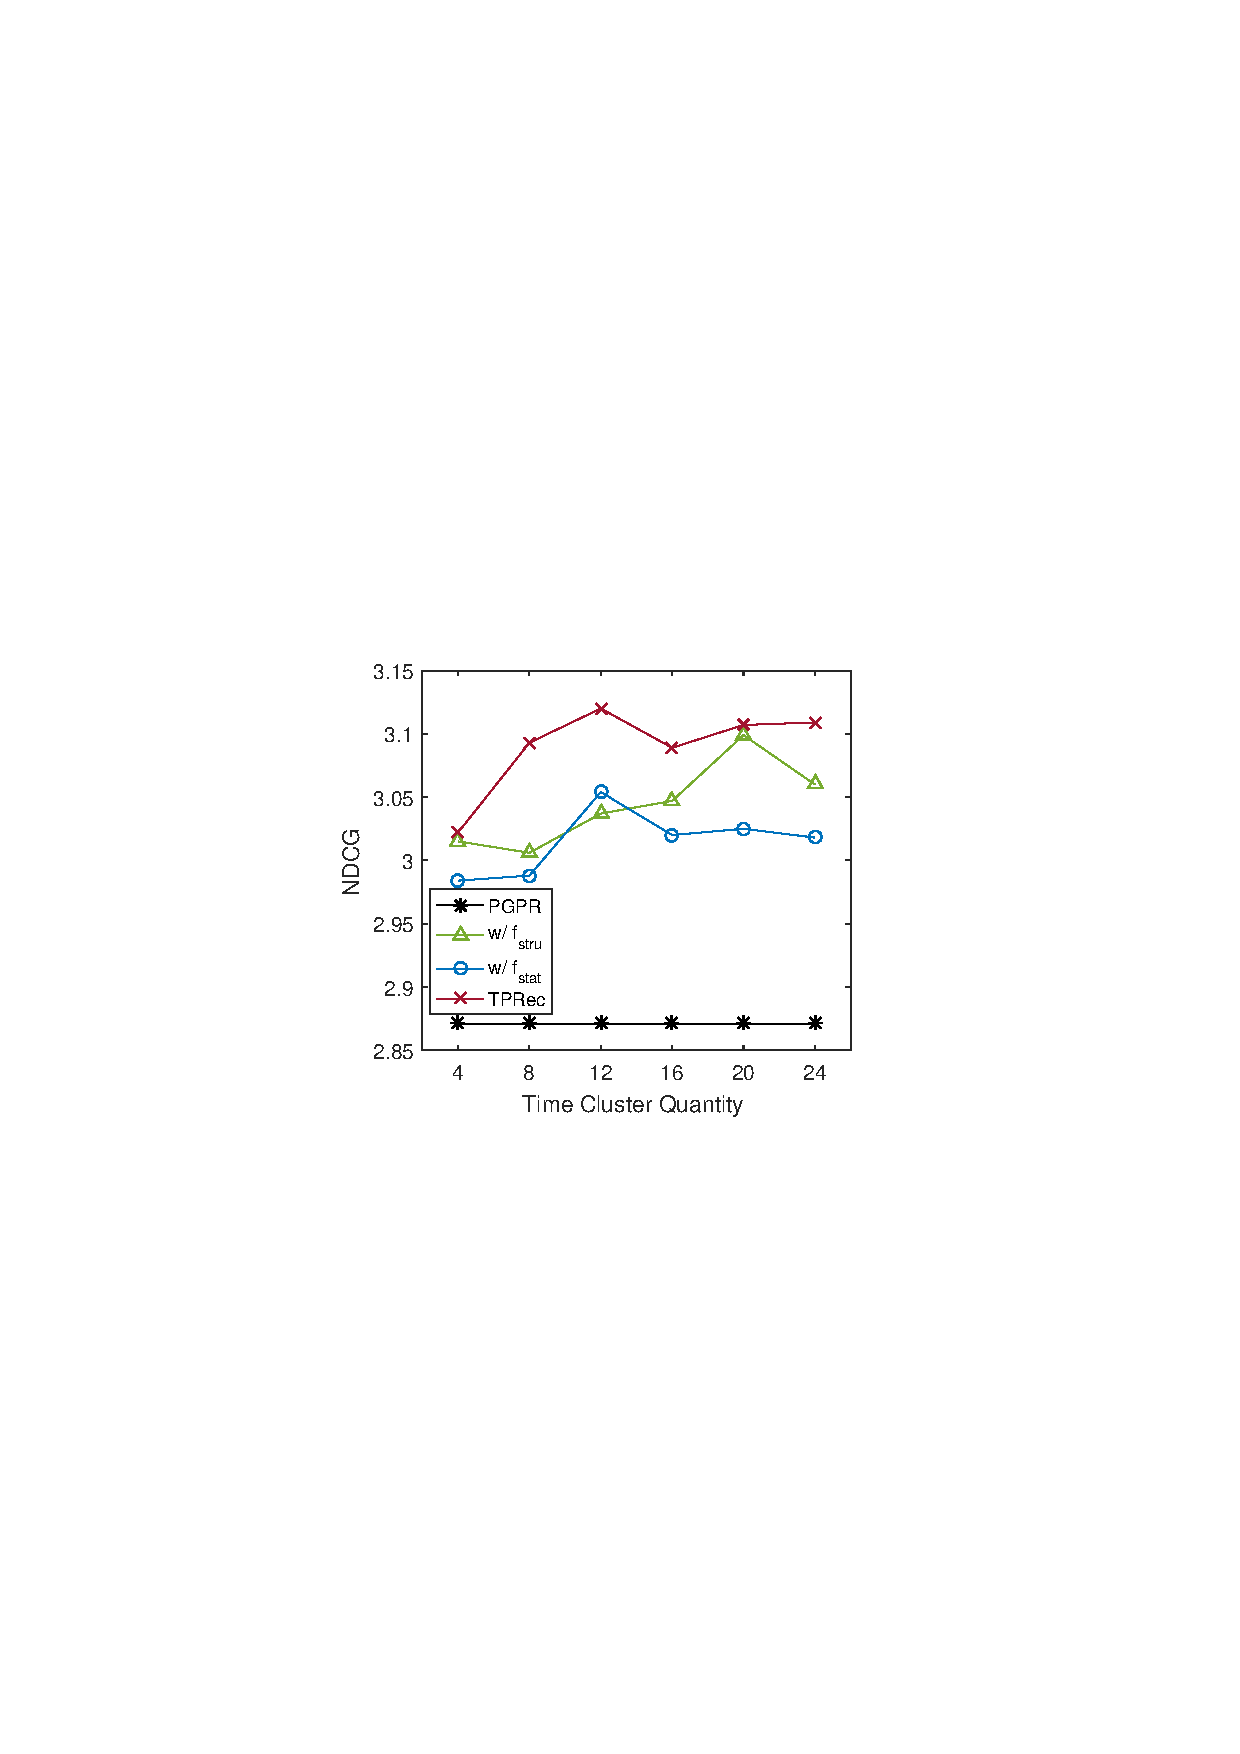
\includegraphics[width=1\textwidth]{chart/cloth_c_ndcg.pdf}
		\end{minipage}
	}
	\subfloat[Recall (Clothing).]{
		\begin{minipage}[t]{0.25\textwidth}
			\centering
			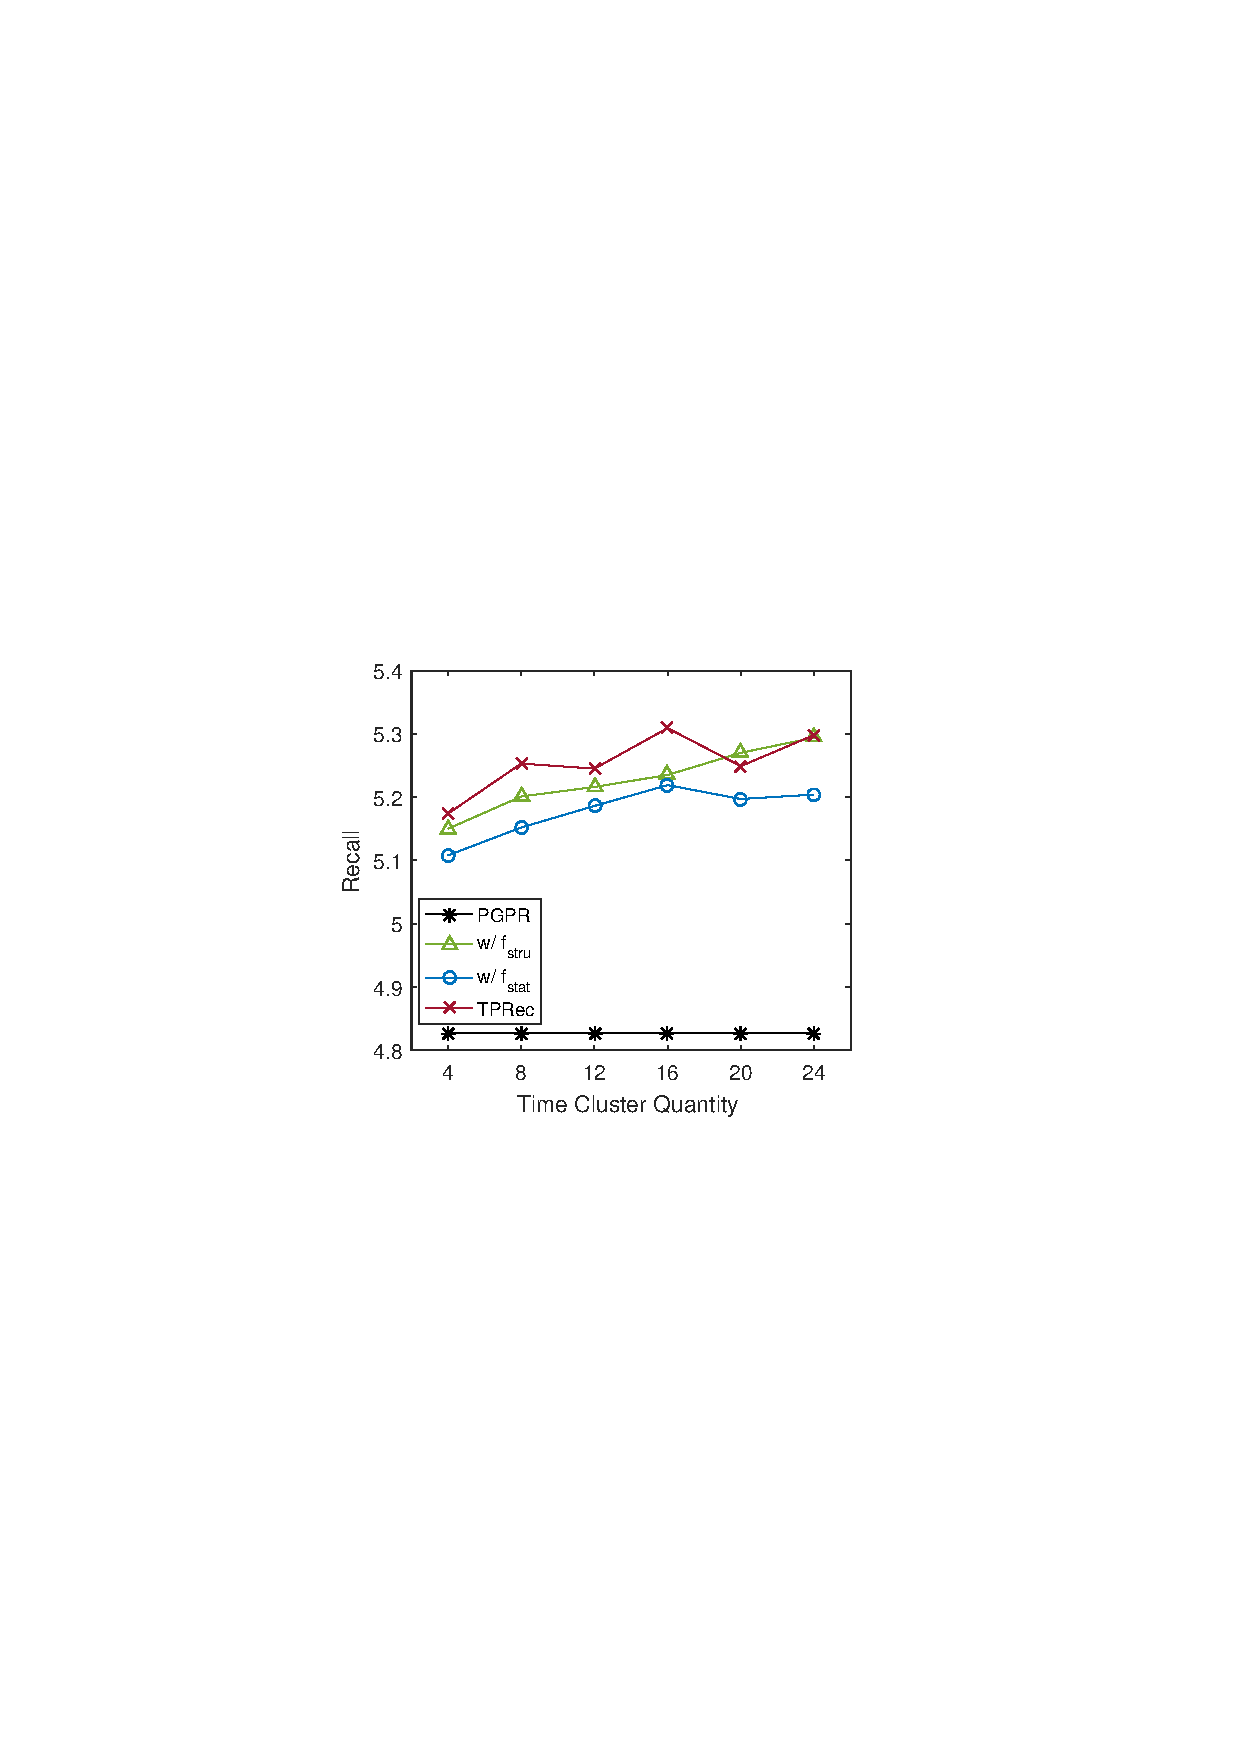
\includegraphics[width=1\textwidth]{chart/cloth_c_recall.pdf}
		\end{minipage}
	}
	\subfloat[HR (Clothing).]{
		\begin{minipage}[t]{0.25\textwidth}
			\centering
			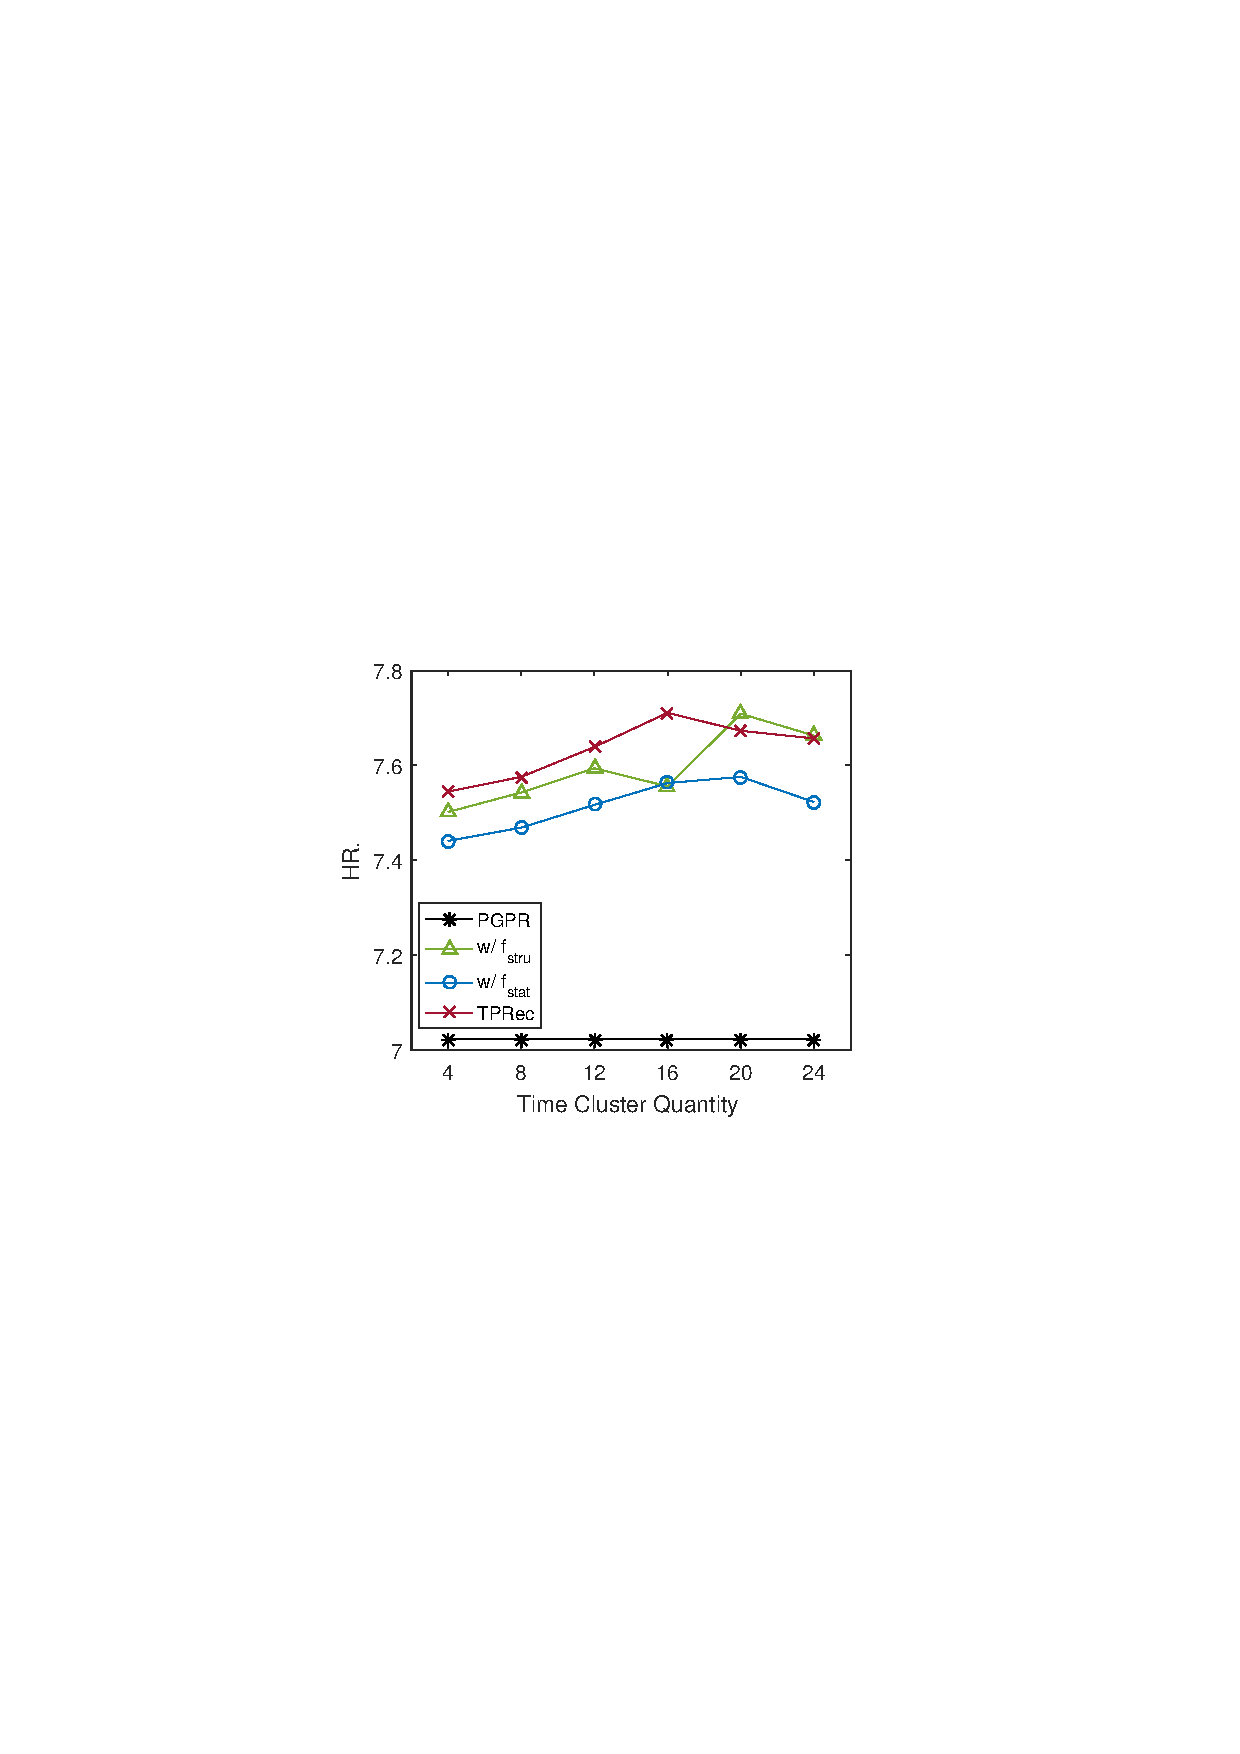
\includegraphics[width=1\textwidth]{chart/cloth_c_hr.pdf}
		\end{minipage}
	}
	\subfloat[Precision (Clothing).]{
		\begin{minipage}[t]{0.25\textwidth}
			\centering
			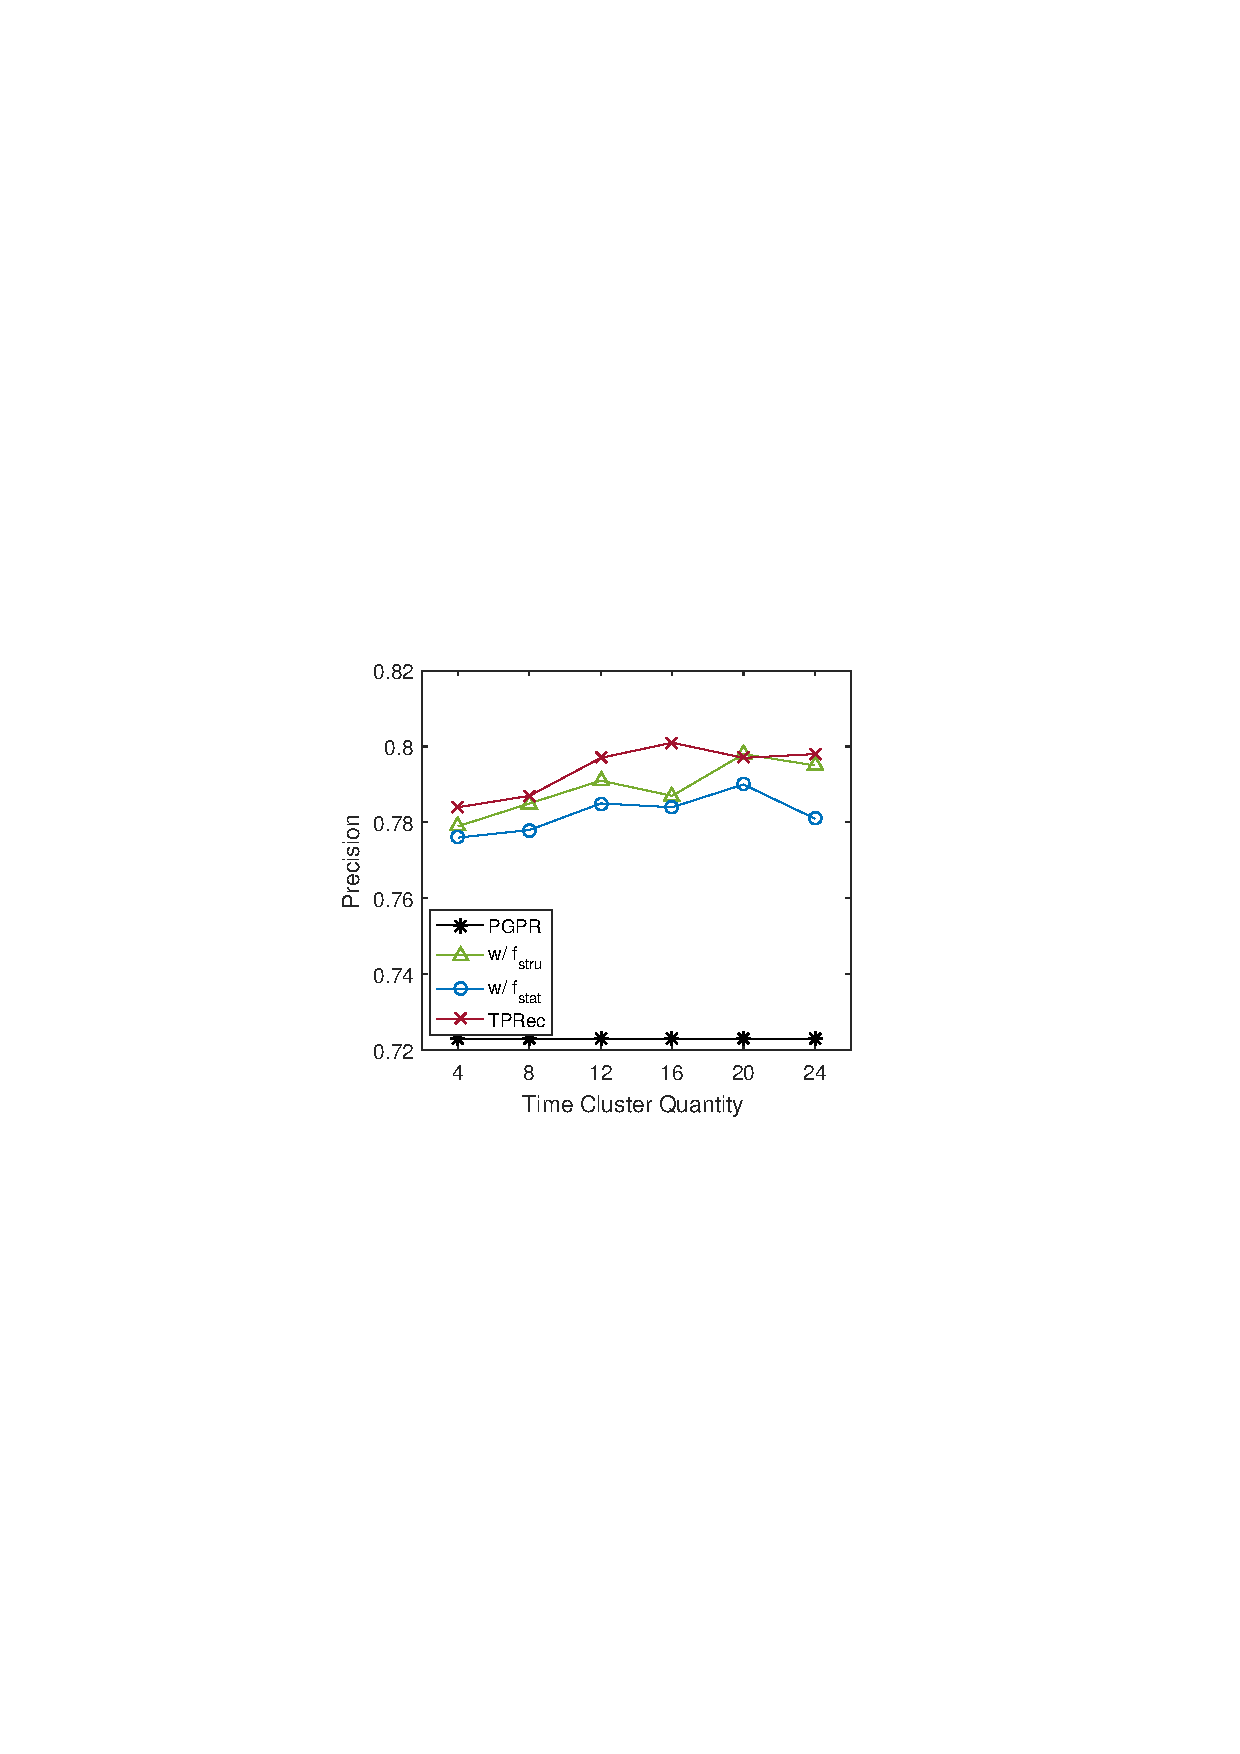
\includegraphics[width=1\textwidth]{chart/cloth_c_prec.pdf}
		\end{minipage}
	}
	
	\subfloat[NDCG (Clothing).]{
		\begin{minipage}[t]{0.25\textwidth}
			\centering
			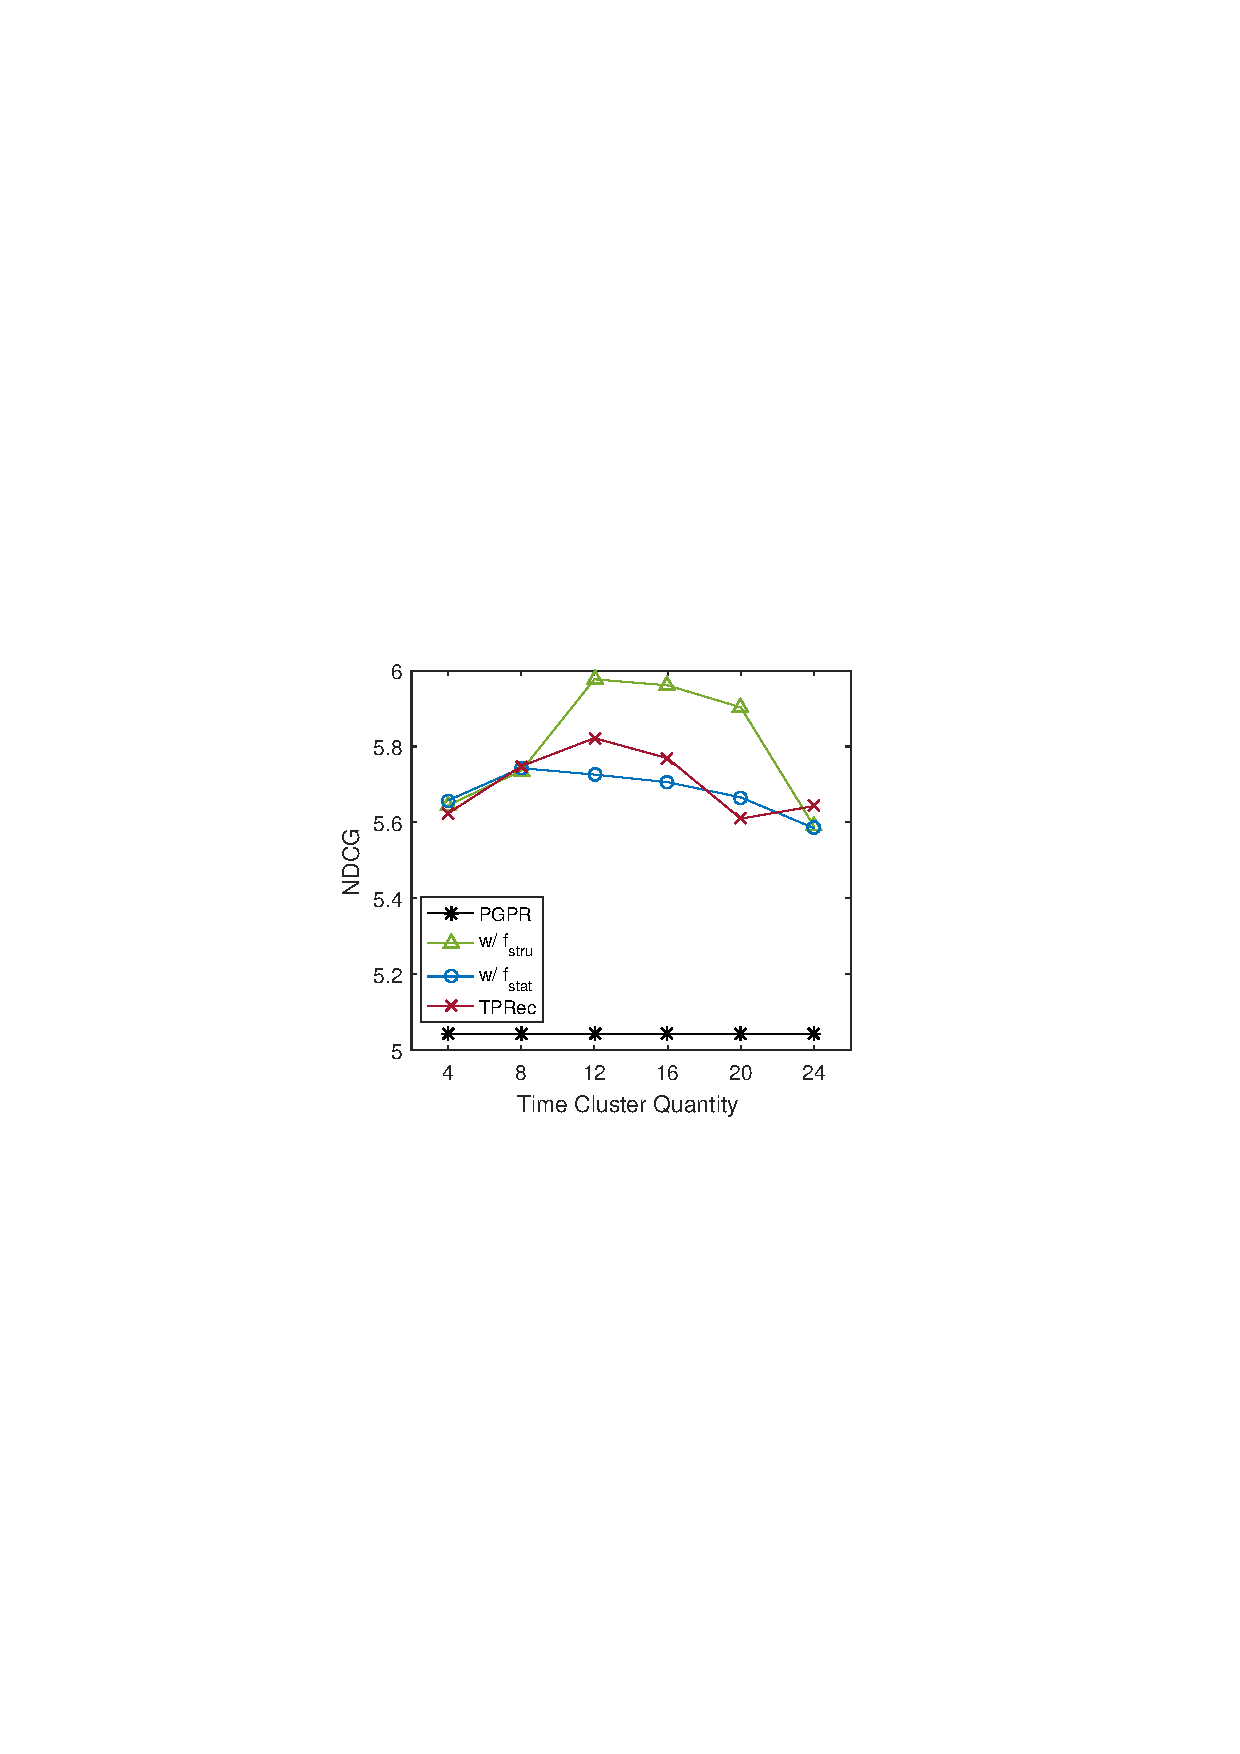
\includegraphics[width=1\textwidth]{chart/cell_c_ndcg.pdf}
		\end{minipage}
	}
	\subfloat[Recall (Cell).]{
		\begin{minipage}[t]{0.25\textwidth}
			\centering
			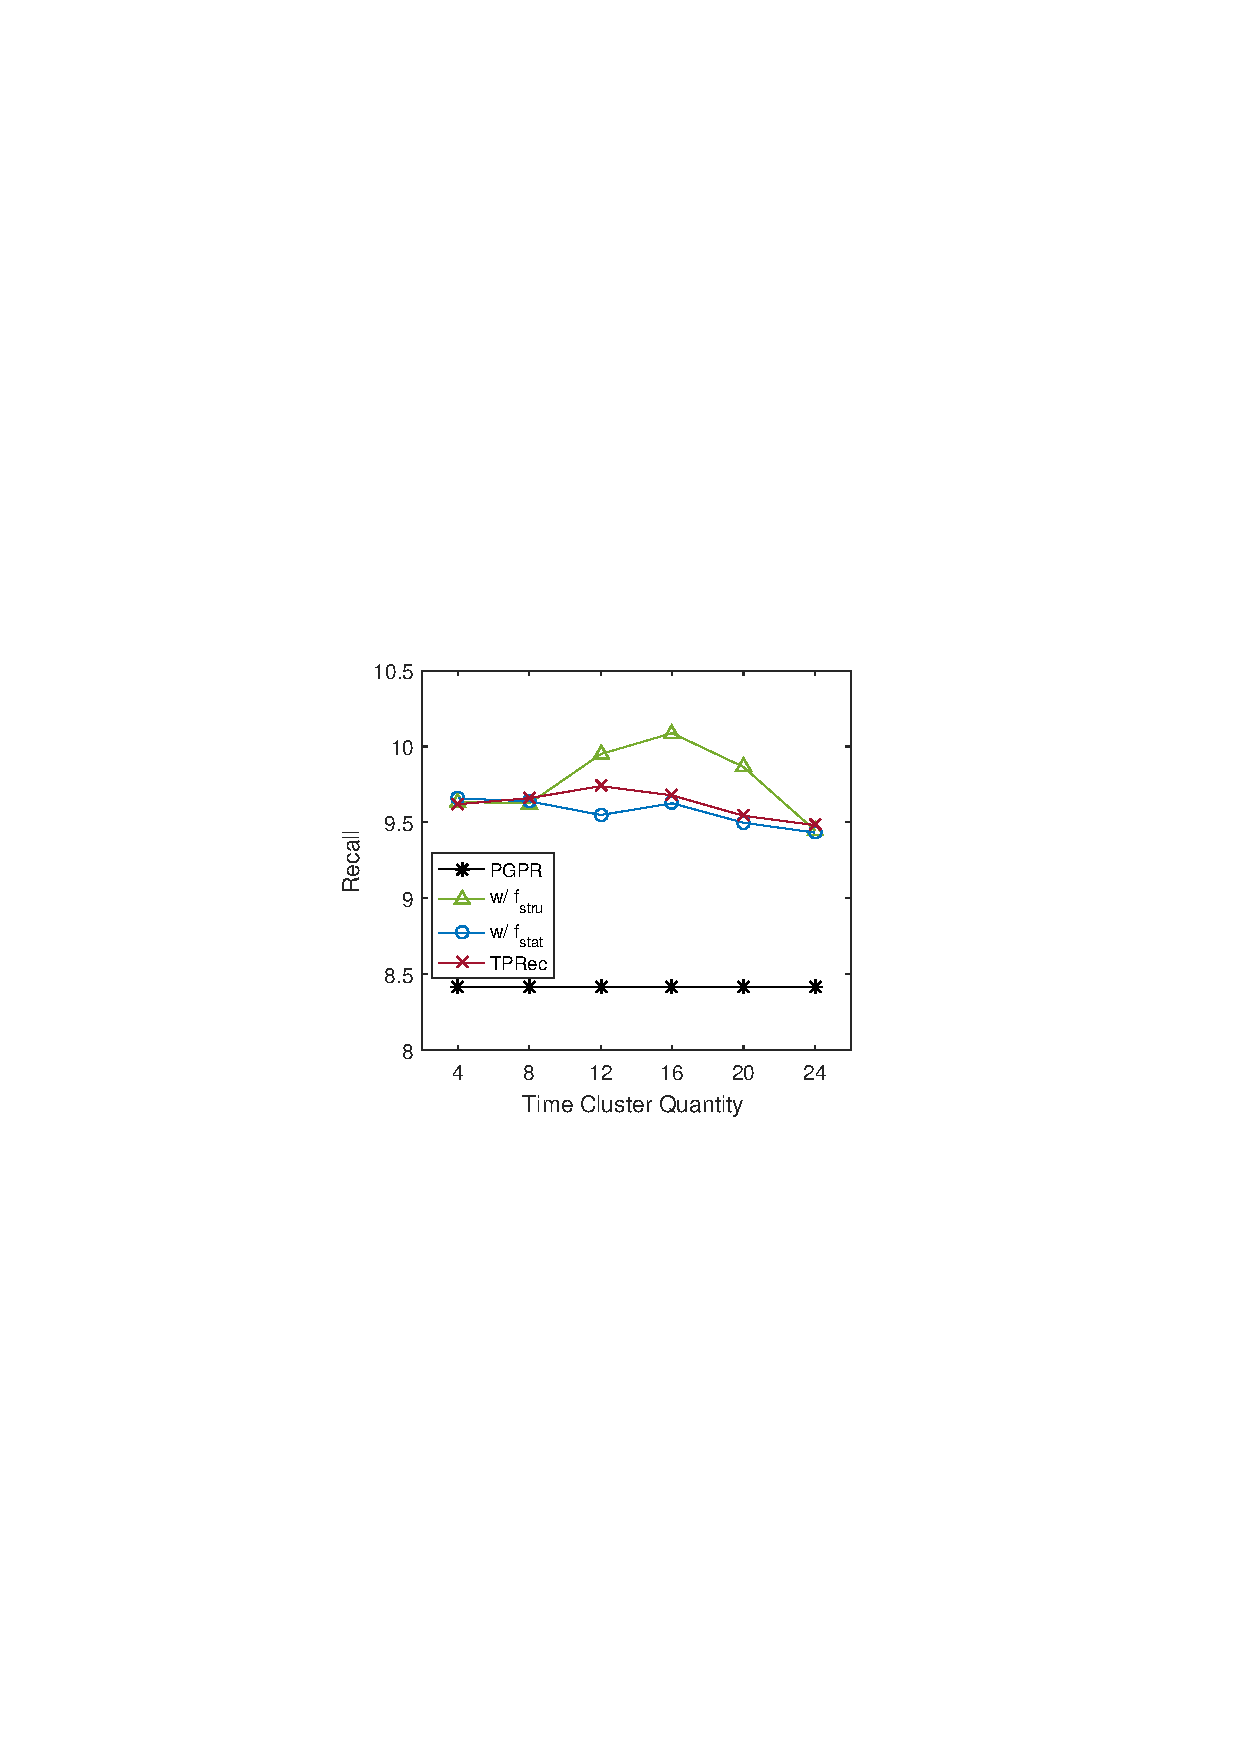
\includegraphics[width=1\textwidth]{chart/cell_c_recall.pdf}
		\end{minipage}
	}
	\subfloat[HR (Cell).]{
		\begin{minipage}[t]{0.25\textwidth}
			\centering
			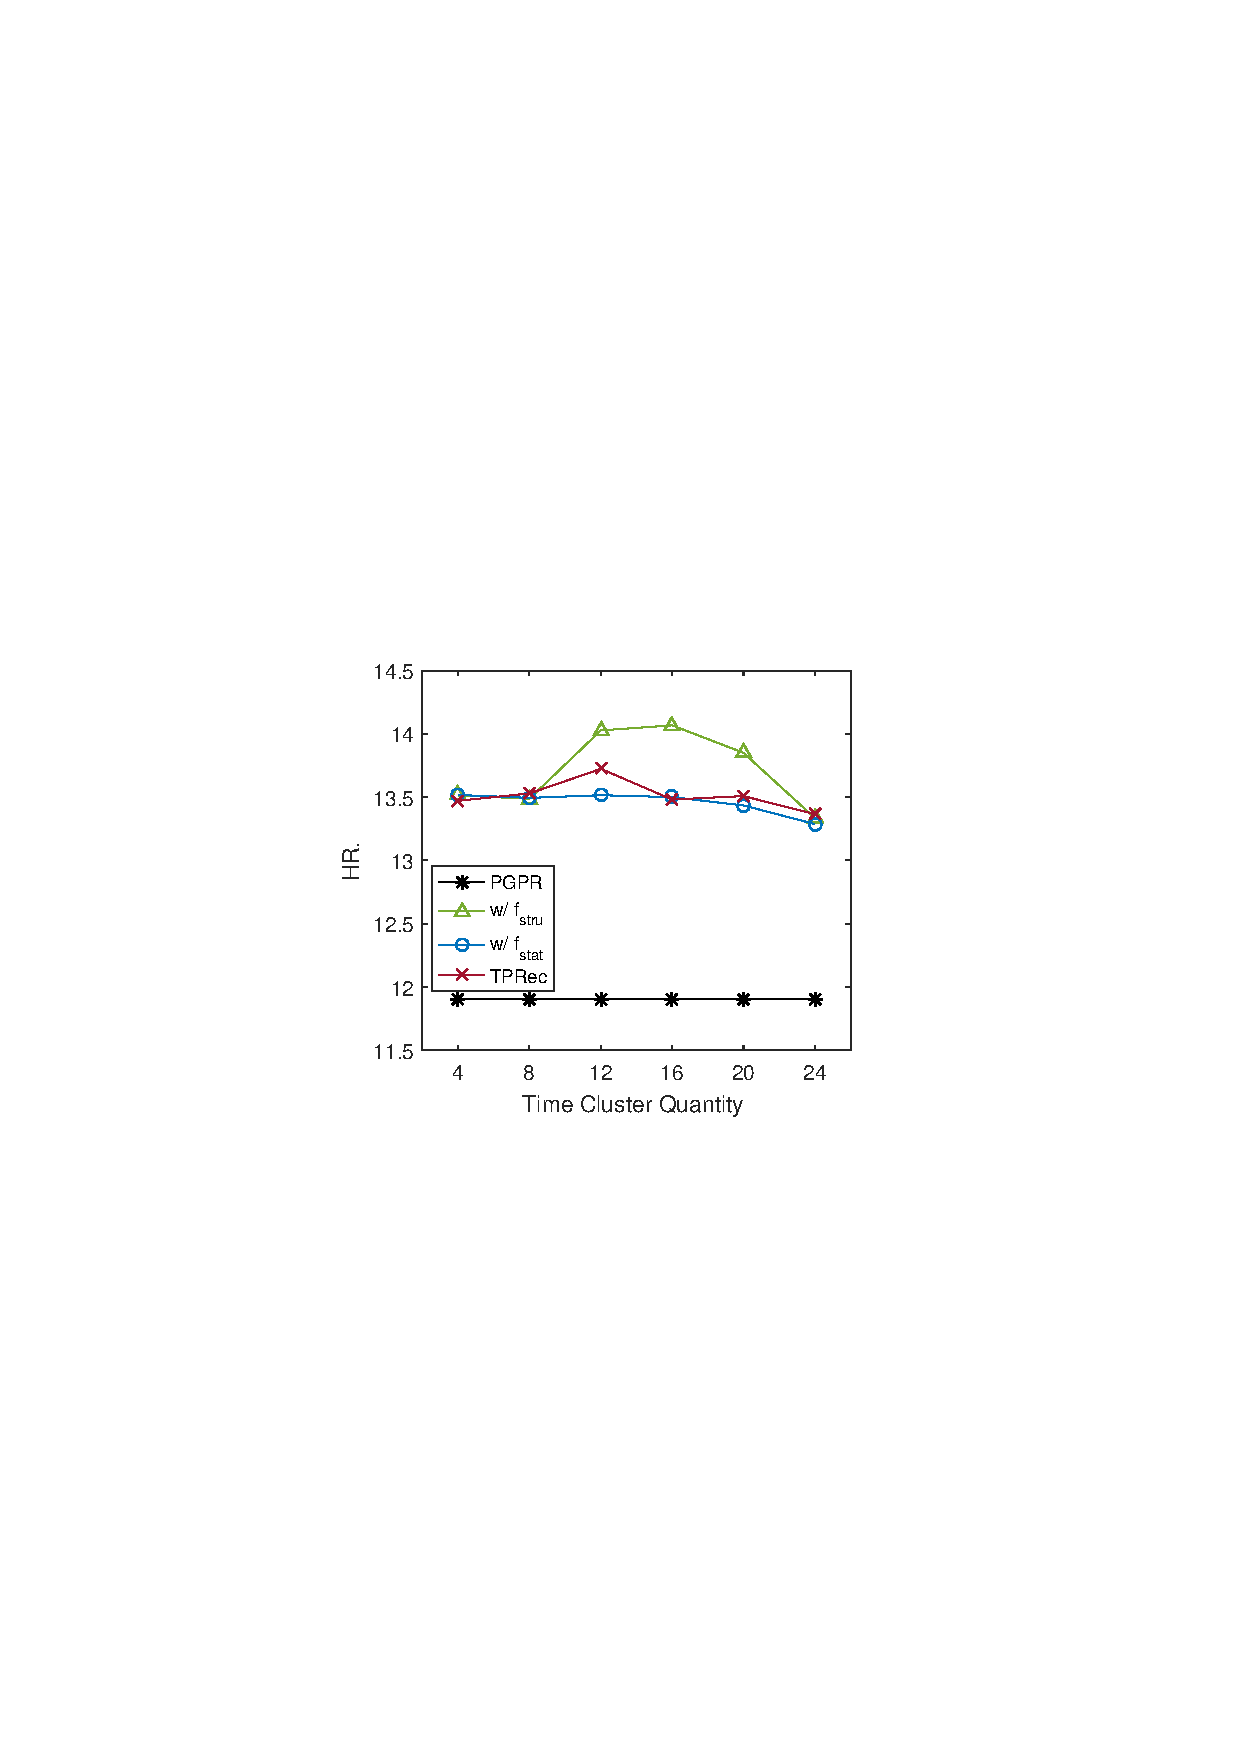
\includegraphics[width=1\textwidth]{chart/cell_c_hr.pdf}
		\end{minipage}
	}
	\subfloat[Precision (Cell).]{
		\begin{minipage}[t]{0.25\textwidth}
			\centering
			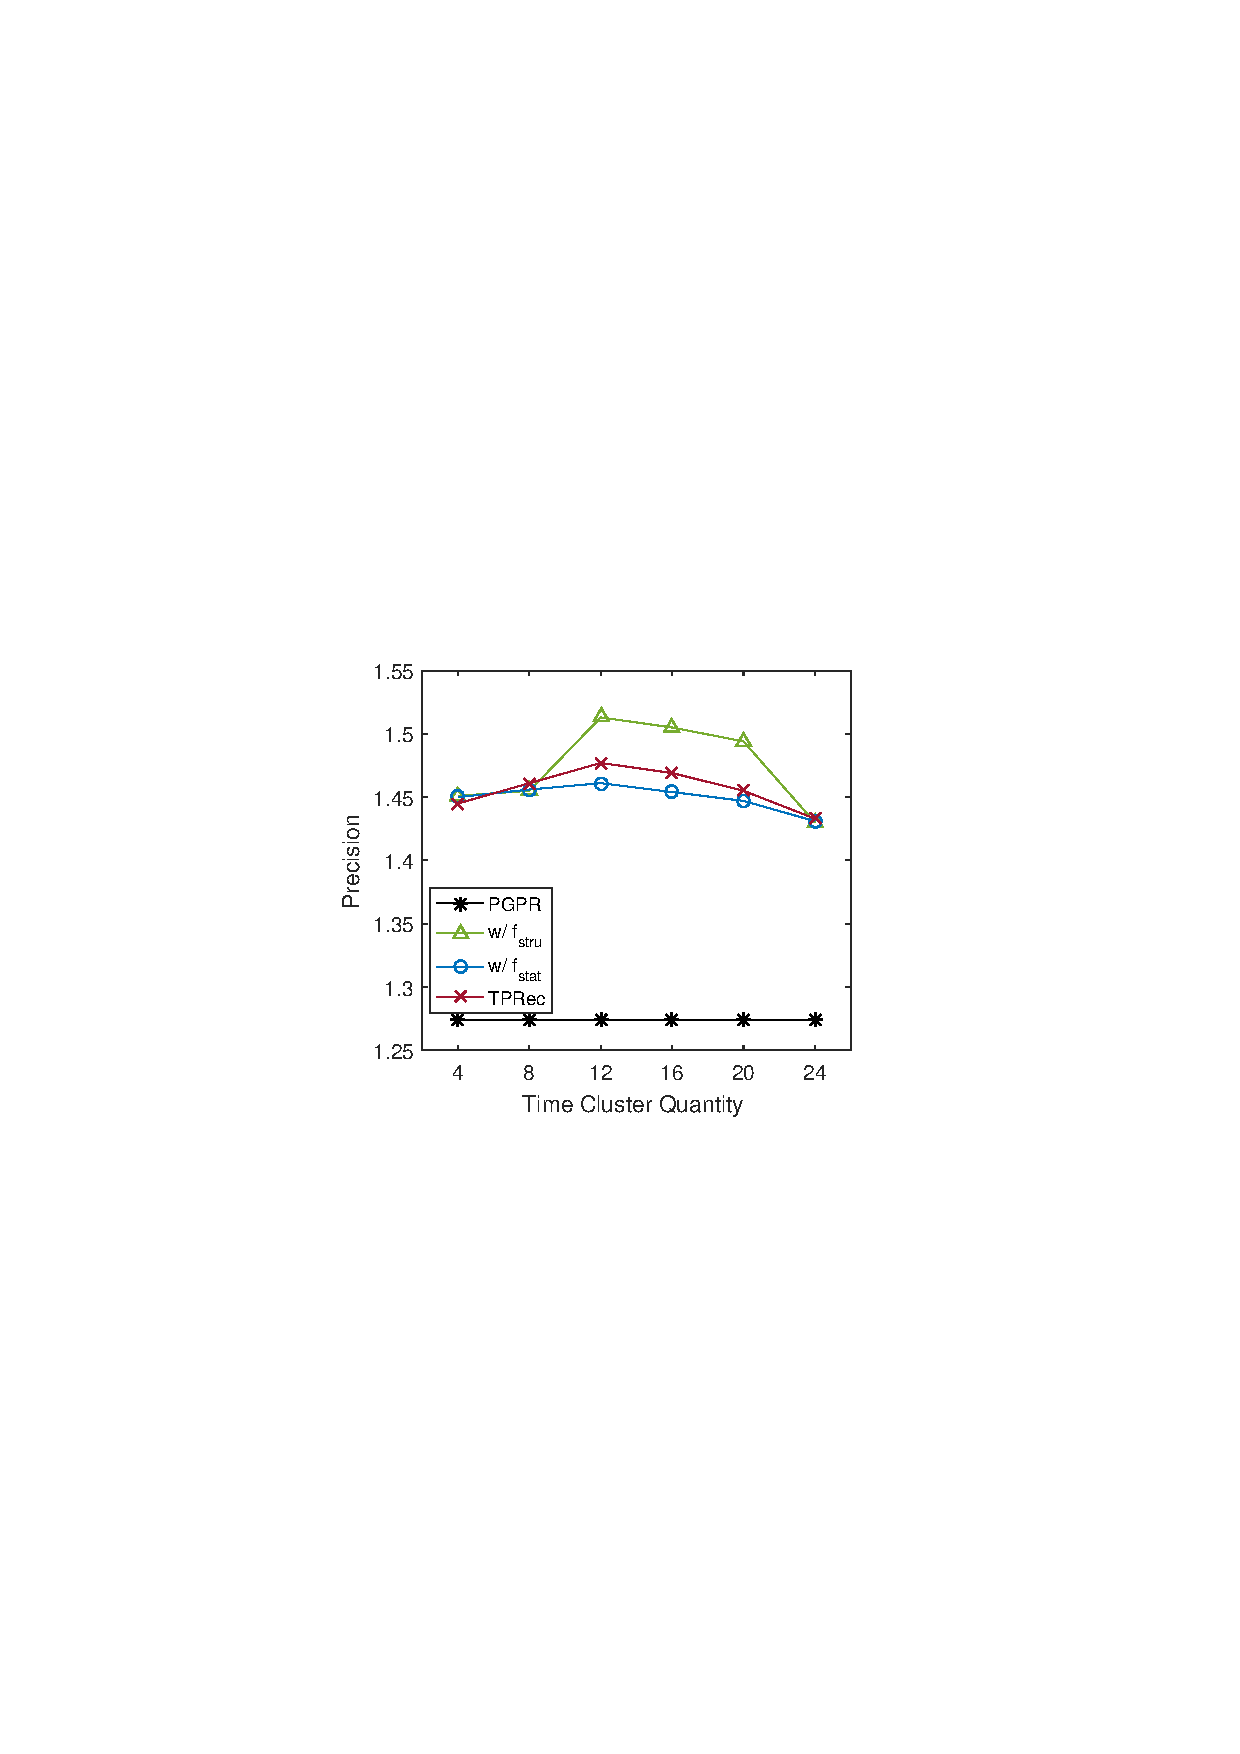
\includegraphics[width=1\textwidth]{chart/cell_c_prec.pdf}
		\end{minipage}
	}
	
	\subfloat[NDCG (Beauty).]{
		\begin{minipage}[t]{0.25\textwidth}
			\centering
			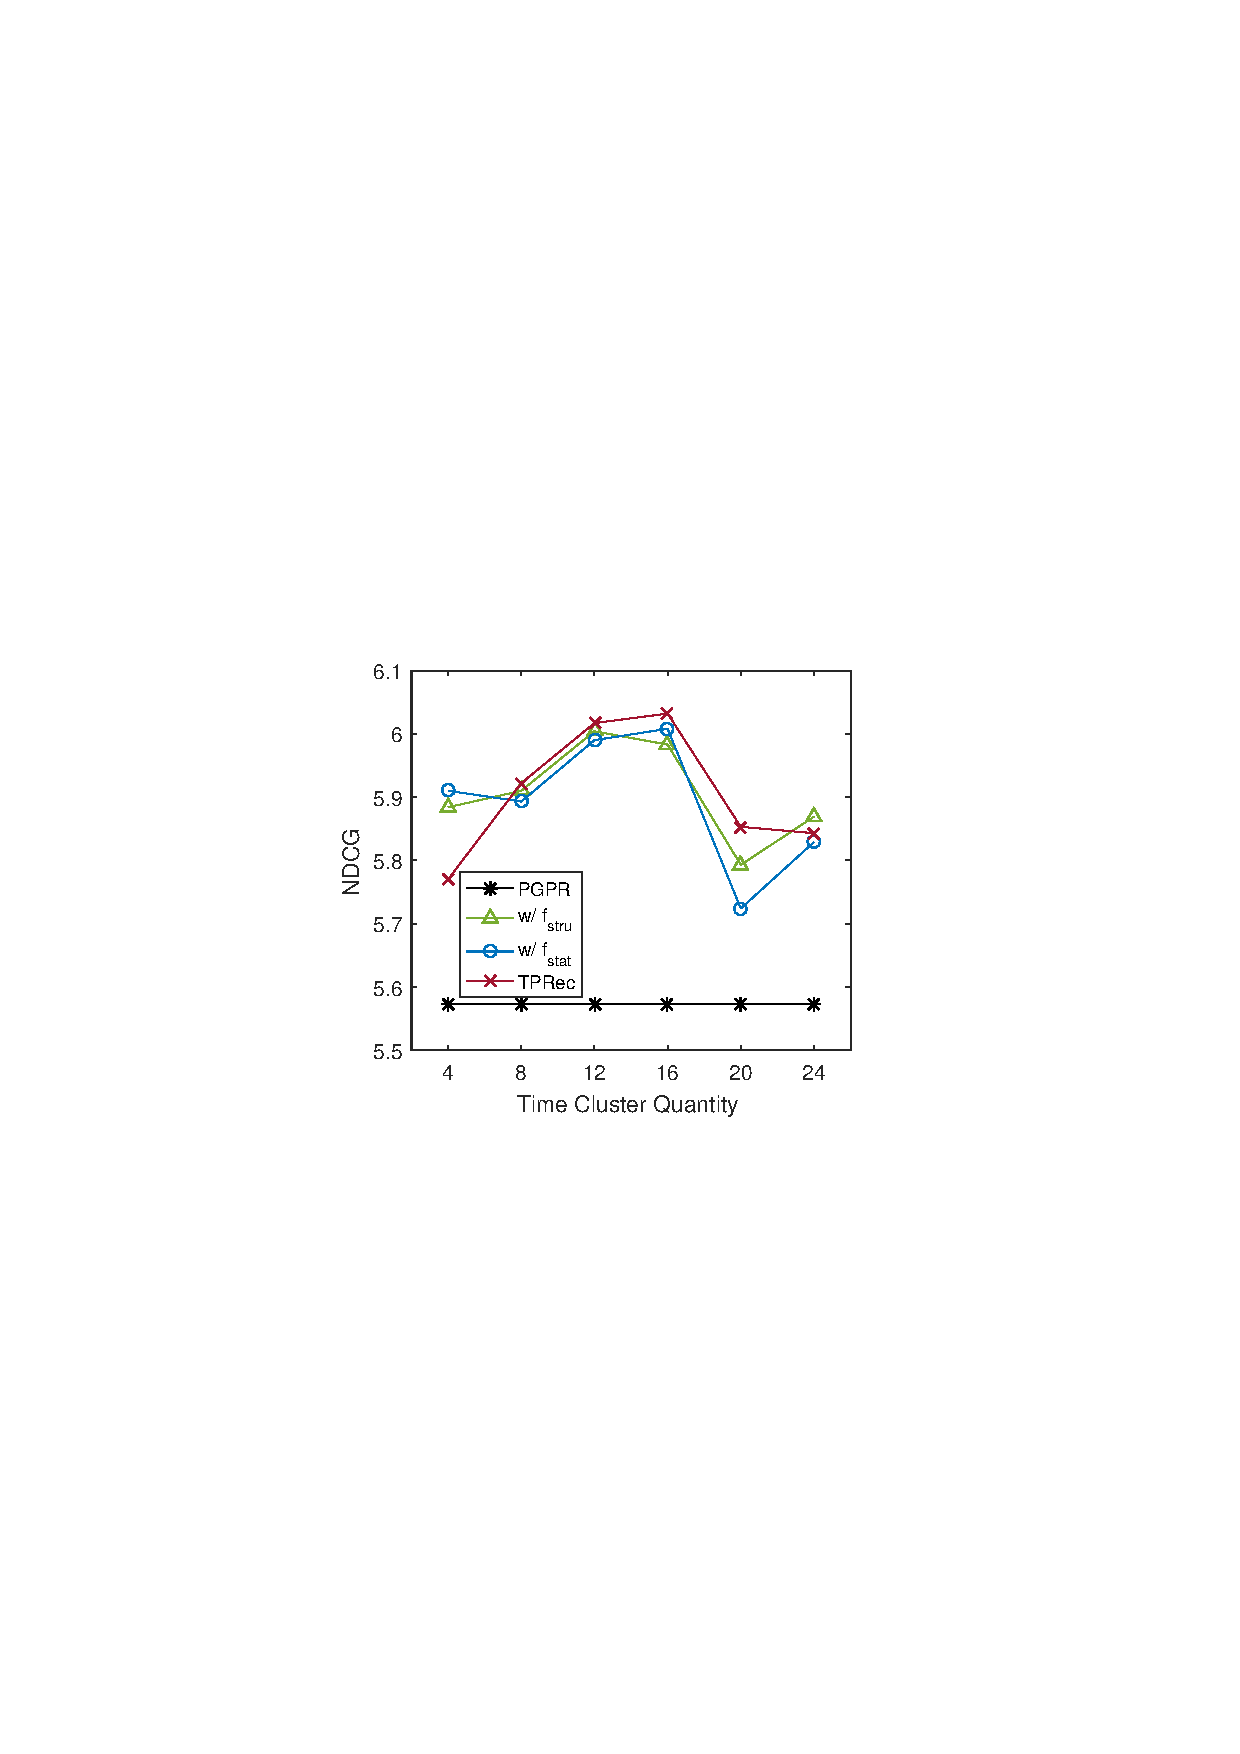
\includegraphics[width=1\textwidth]{chart/beauty_c_ndcg.pdf}
		\end{minipage}
	}
		\subfloat[Recall (Beauty).]{
		\begin{minipage}[t]{0.25\textwidth}
			\centering
			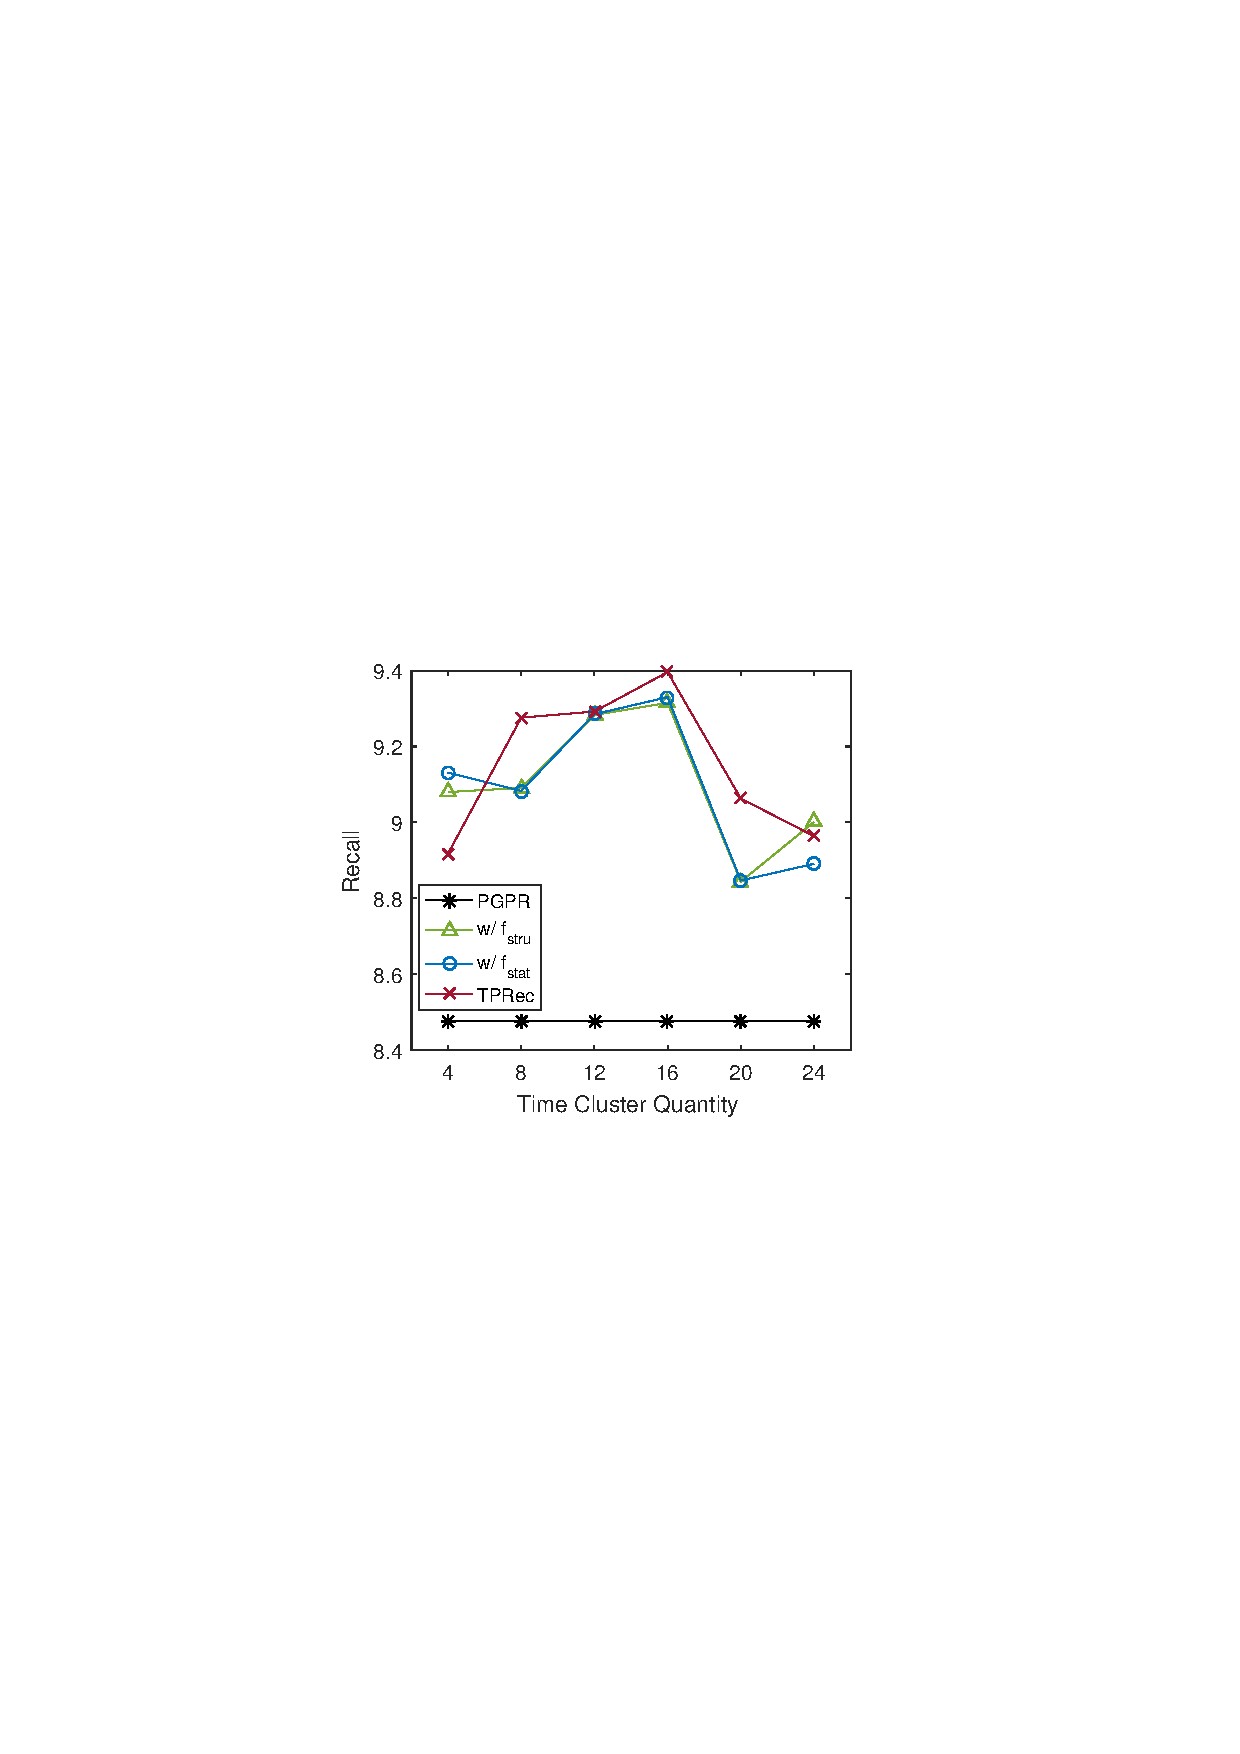
\includegraphics[width=1\textwidth]{chart/beauty_c_recall.pdf}
		\end{minipage}
	}
	\subfloat[HR (Beauty).]{
		\begin{minipage}[t]{0.25\textwidth}
			\centering
			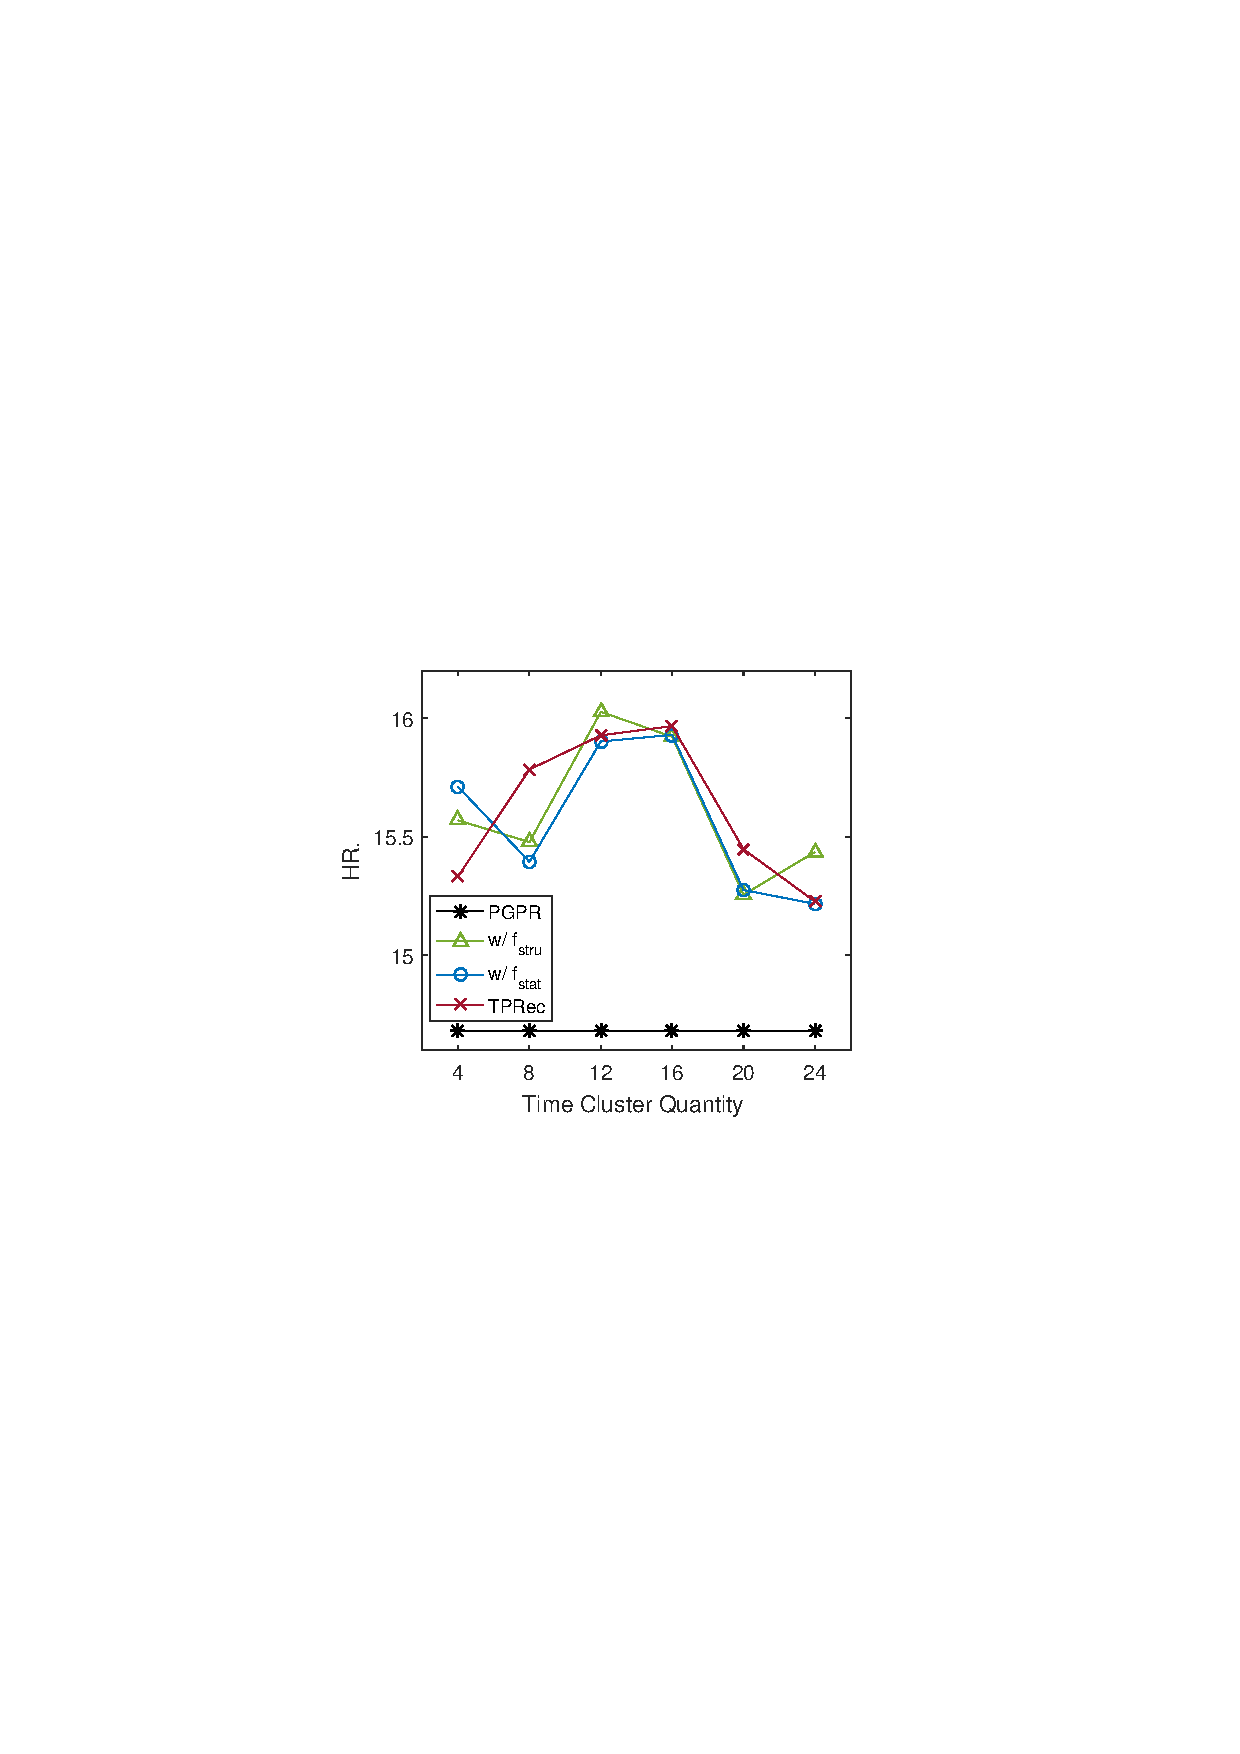
\includegraphics[width=1\textwidth]{chart/beauty_c_hr.pdf}
		\end{minipage}
	}
	\subfloat[Precision (Beauty).]{
		\begin{minipage}[t]{0.25\textwidth}
			\centering
			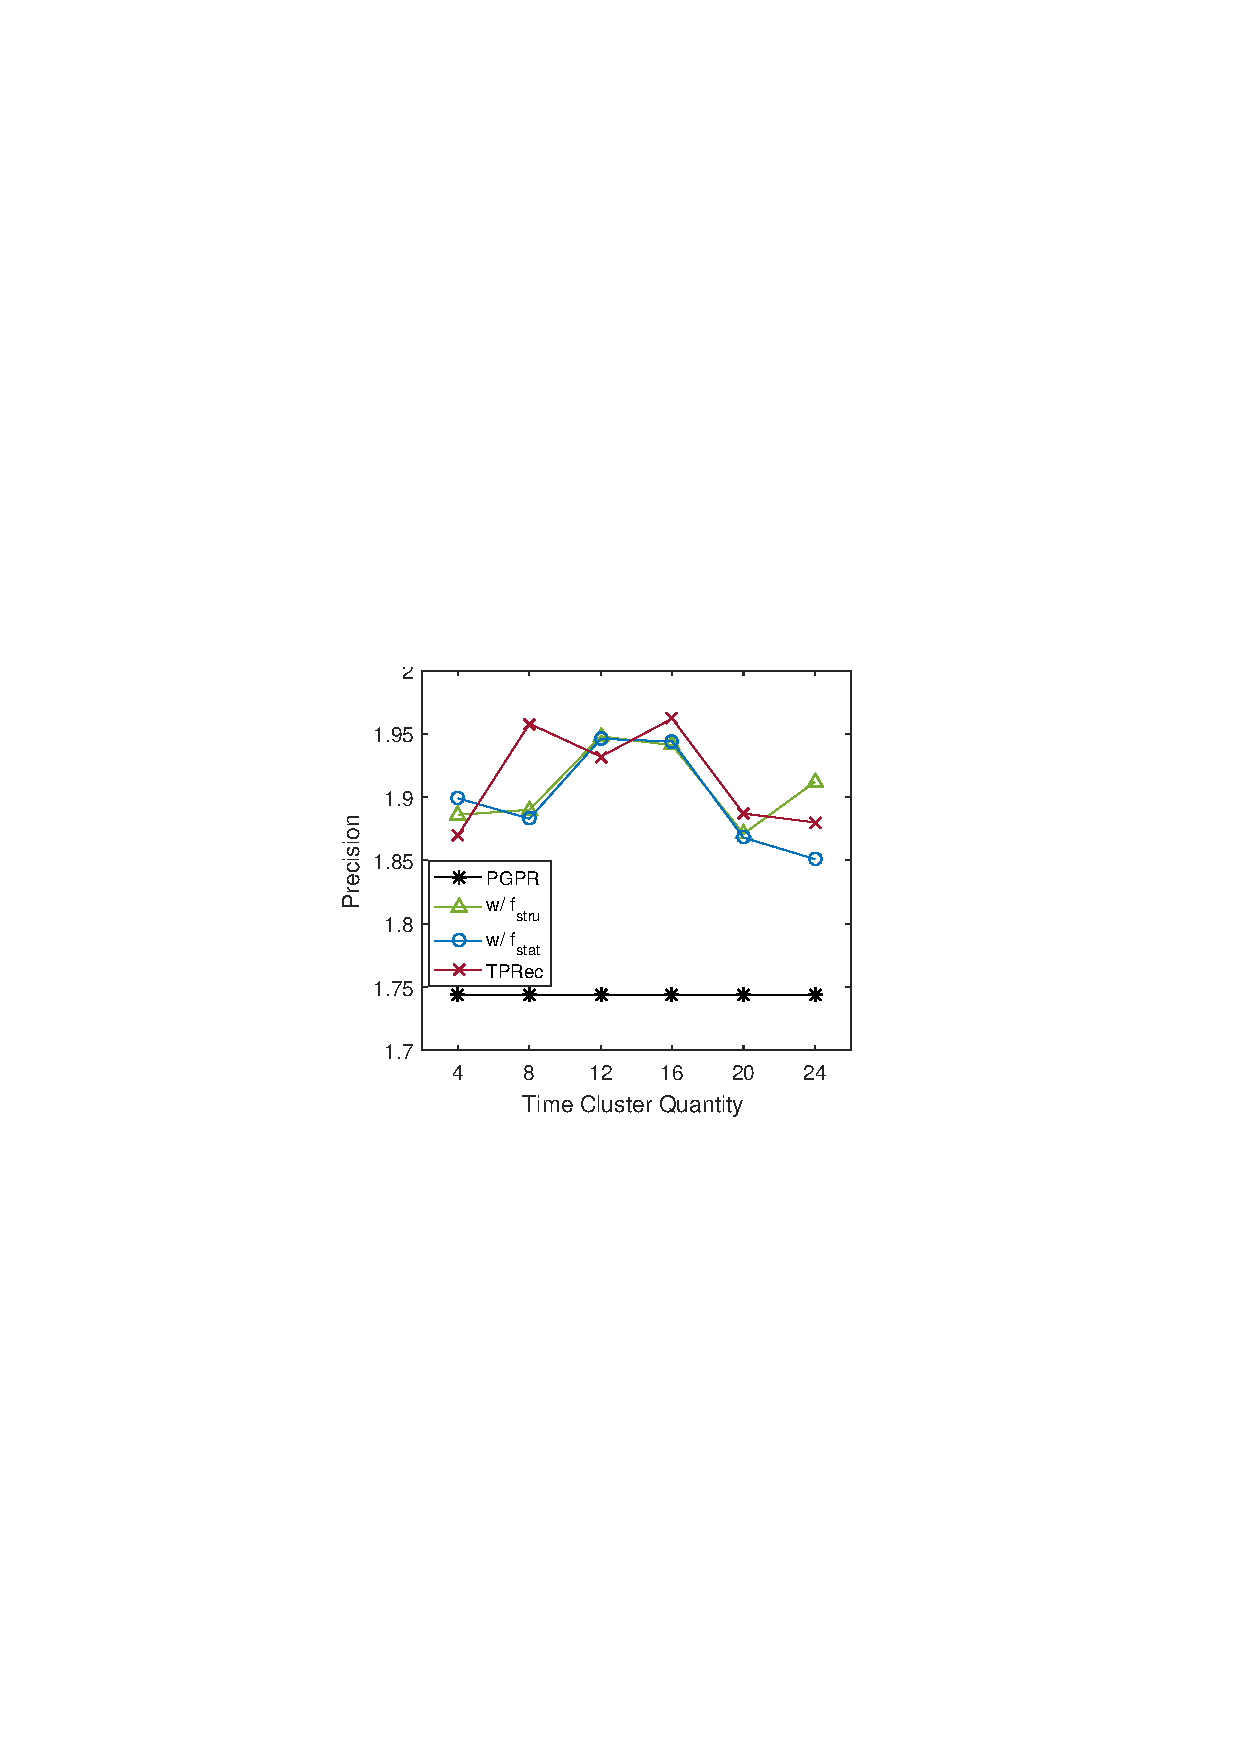
\includegraphics[width=1\textwidth]{chart/beauty_c_prec.pdf}
		\end{minipage}
	}
\caption{ Effect of varying time cluster quantity $L$.
}
	\label{cluster_num}
\end{figure}

\subsubsection{\textbf{Effect of Action Space Size.}}
 Figure \ref{actionSpace} presents the performance of four compared methods with different action space size $\epsilon$ varying from 100 to 500. We make the following two observations: 
  (1) With few exceptions, all three versions of \tkgrec\ consistently outperform PGPR with various $\epsilon$, demonstrating the effectiveness of exploiting temporal information. 
(2) As the action space size $\epsilon$ increases, generally speaking, the performance will become better at the beginning.  The reason is that when the action space size $\epsilon$ is too small, the model is likely to miss the relevant paths. It also can be seen from Figure \ref{act_invalid}, that a smaller action space size (\eg\ $ \epsilon\leq 200$) would incur a larger number of invalid users.
 %
 (3) But when the $\epsilon$ surpasses a certain threshold, the performance of all the methods drops with $\epsilon$ further increasing. The reason is that a larger action space would increase the risk of retrieving irrelevant paths. Nonetheless, our \tkgrec\ drops relatively mildly. It demonstrates our \tkgrec\ is more robust to $\epsilon$ and able to identify high-quality paths by leveraging temporal information. 
 
 
 %Also, we find the smallest $\epsilon$ may not bring optimal performance. It can be seen from the inferior performance of some methods with $\epsilon=100$ comparing with $\epsilon=150$. 
 %Therefore, we adopt the maximum size of action space as $|\mathcal{A}_k| = \epsilon \leq250$ as PGPR\cite{pgpr} do to get a suitable performance in Section \ref{rq1}.

%To explore the impact of action space size, we consider to set the action space size by 50 margin ranging from 100 to 500. Recall that action space size $\epsilon$ is defined in Equation \ref{actionprun}, which means for a user $u$ at step $k$, only the top $\epsilon$ relations from the pruning function $g_k((r,e_{k+1}) \, |\, u)$ could be selected as action candidates.
%%
%In other words, a smaller action space might cause the RL agent miss the correct path, while larger action space means more irrelevant actions will be served to user. This experiment aims to show how does the action space size affects the  performance and which action space size is a better choice.
%%
%We experiment on three datasets Clothing, Cell Phones and Beauty, and report the performance of w/o $\boldsymbol{f_{stat}}$,
%w/o $\boldsymbol{f_{stat}}$ and \tkgrec. What's more, the baseline method PGPR is also reported for comparison. The results are plotted in Figure \ref{actionSpace}, and we have the following observations:
%
%\begin{itemize}
%\item Our model \tkgrec, including two variants (w/o $\boldsymbol{f_{stat}}$,
%w/o $\boldsymbol{f_{stat}}$), outperform PGPR under most choices of action space sizes.
%%
%As shown in Figure \ref{actionSpace}, the black curve of PGPR is consistently under other curves for all sizes ranging from 100 to 500. It again verifies the effectiveness of our time-aware path reasoning compared to other baselines.
%
%\item As illustrated in Figure \ref{actionSpace}, the common trend is that a smaller action space size leads to better performance, but too small action space may hurt the diversity of the recommendation results when performing path reasoning.
%%
%It's obvious that the performance of PGPR decreases rapidly while the action space size increases. Whereas, the performance of our model is slightly influenced by the action space size.
%%
%This means that though larger action space could bring more irrelevant actions to user, our scoring function based on original relations $r_{kg}$ and time-aware interaction relations $r_{interact}$ can select higher-quality actions to avoid lowering the effect.
%
%\end{itemize}

% 后面就巴拉巴拉一通讲啊, 每一个画个图啊, 巴拉巴拉的.

\begin{figure}[]
	\centering
	\subfloat[NDCG (Clothing).]{
		\begin{minipage}[t]{0.25\textwidth}
			\centering
			
\includegraphics[width=1\textwidth]{chart/cloth_ndcg.pdf}
		\end{minipage}
	}
	\subfloat[Recall (Clothing).]{
		\begin{minipage}[t]{0.25\textwidth}
			\centering
			
\includegraphics[width=1\textwidth]{chart/cloth_recall.pdf}
		\end{minipage}
	}
	\subfloat[HR (Clothing).]{
		\begin{minipage}[t]{0.25\textwidth}
			\centering
			
\includegraphics[width=1\textwidth]{chart/cloth_hr.pdf}
		\end{minipage}
	}
	\subfloat[Precision (Clothing).]{
		\begin{minipage}[t]{0.25\textwidth}
			\centering
			
\includegraphics[width=1\textwidth]{chart/cloth_prec.pdf}
		\end{minipage}
	}
	
	\subfloat[NDCG (Cell).]{
		\begin{minipage}[t]{0.25\textwidth}
			\centering
			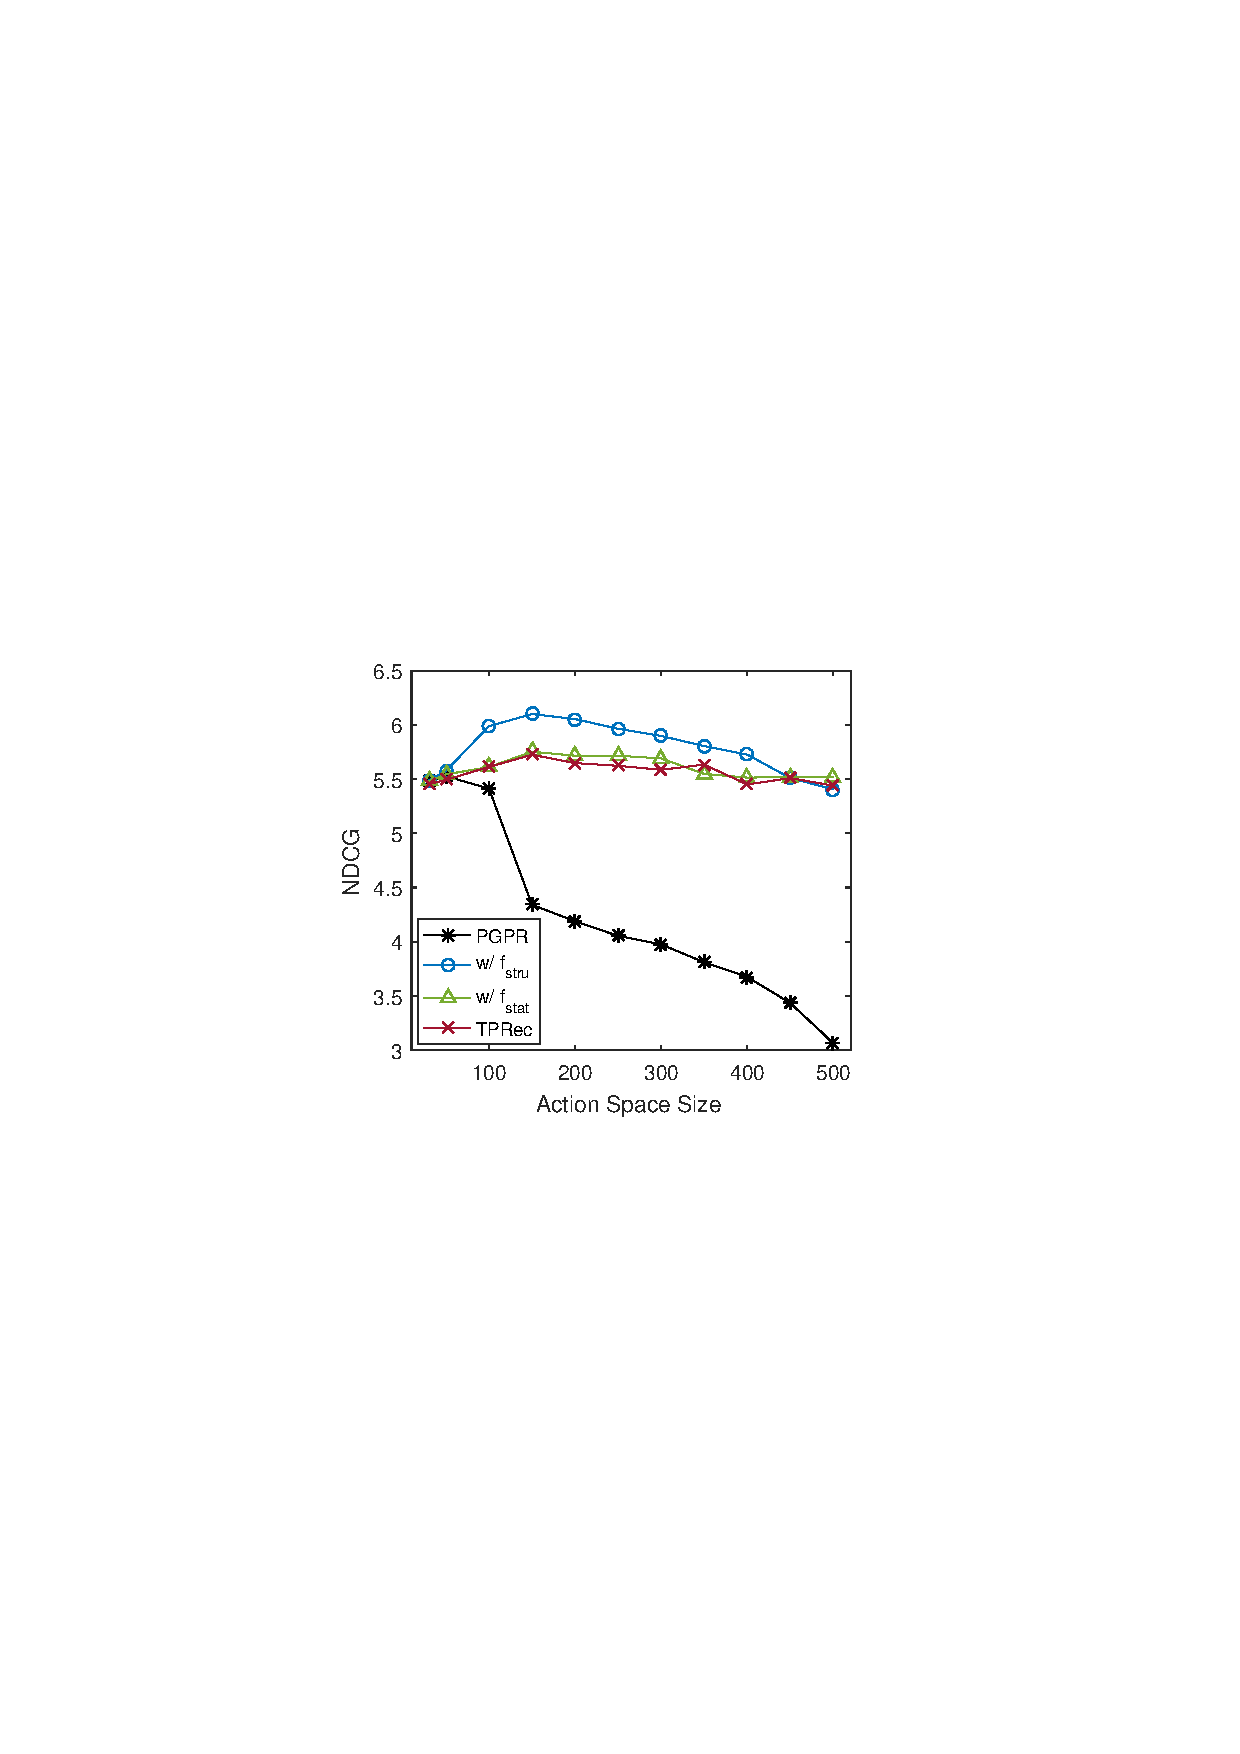
\includegraphics[width=1\textwidth]{chart/cell_ndcg.pdf}
		\end{minipage}
	}
	\subfloat[Recall (Cell).]{
		\begin{minipage}[t]{0.25\textwidth}
			\centering
			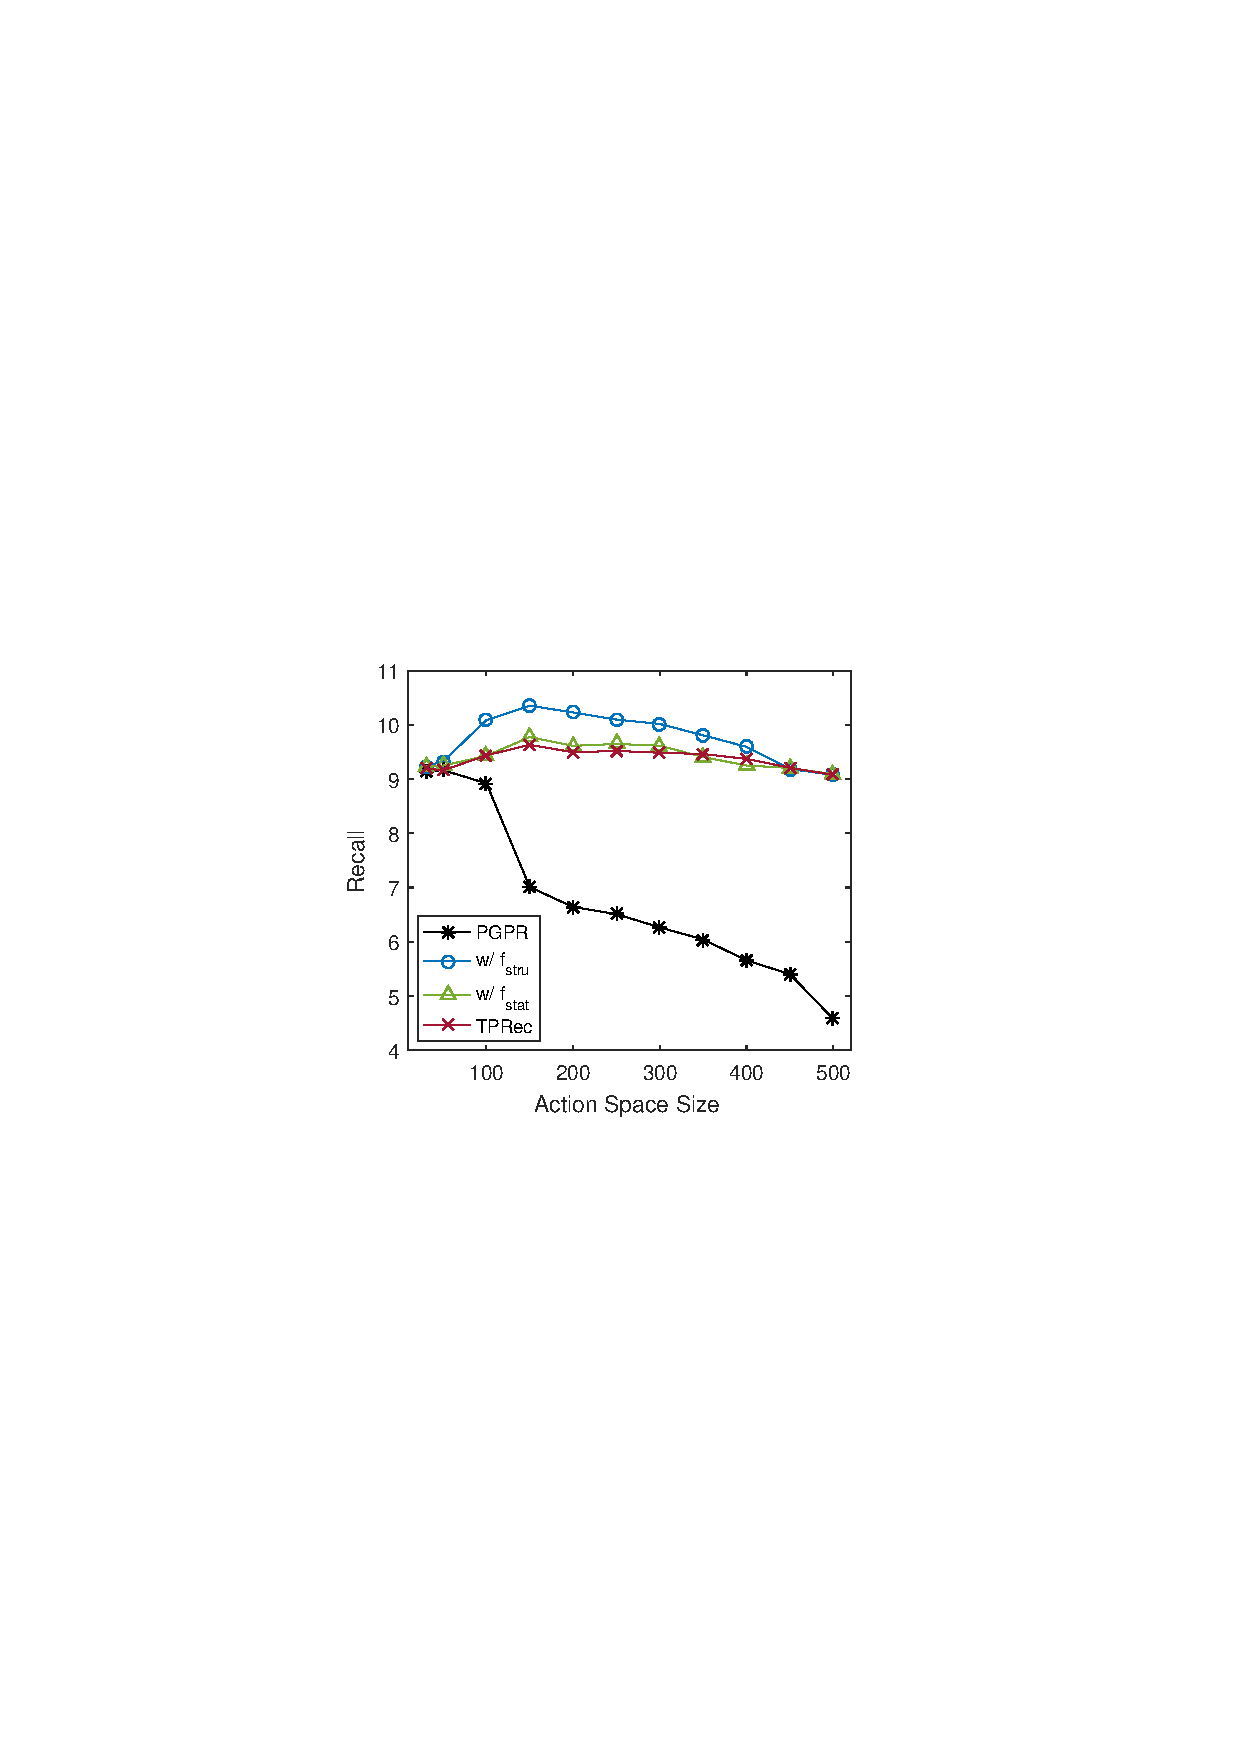
\includegraphics[width=1\textwidth]{chart/cell_recall.pdf}
		\end{minipage}
	}
	\subfloat[HR (Cell).]{
		\begin{minipage}[t]{0.25\textwidth}
			\centering
			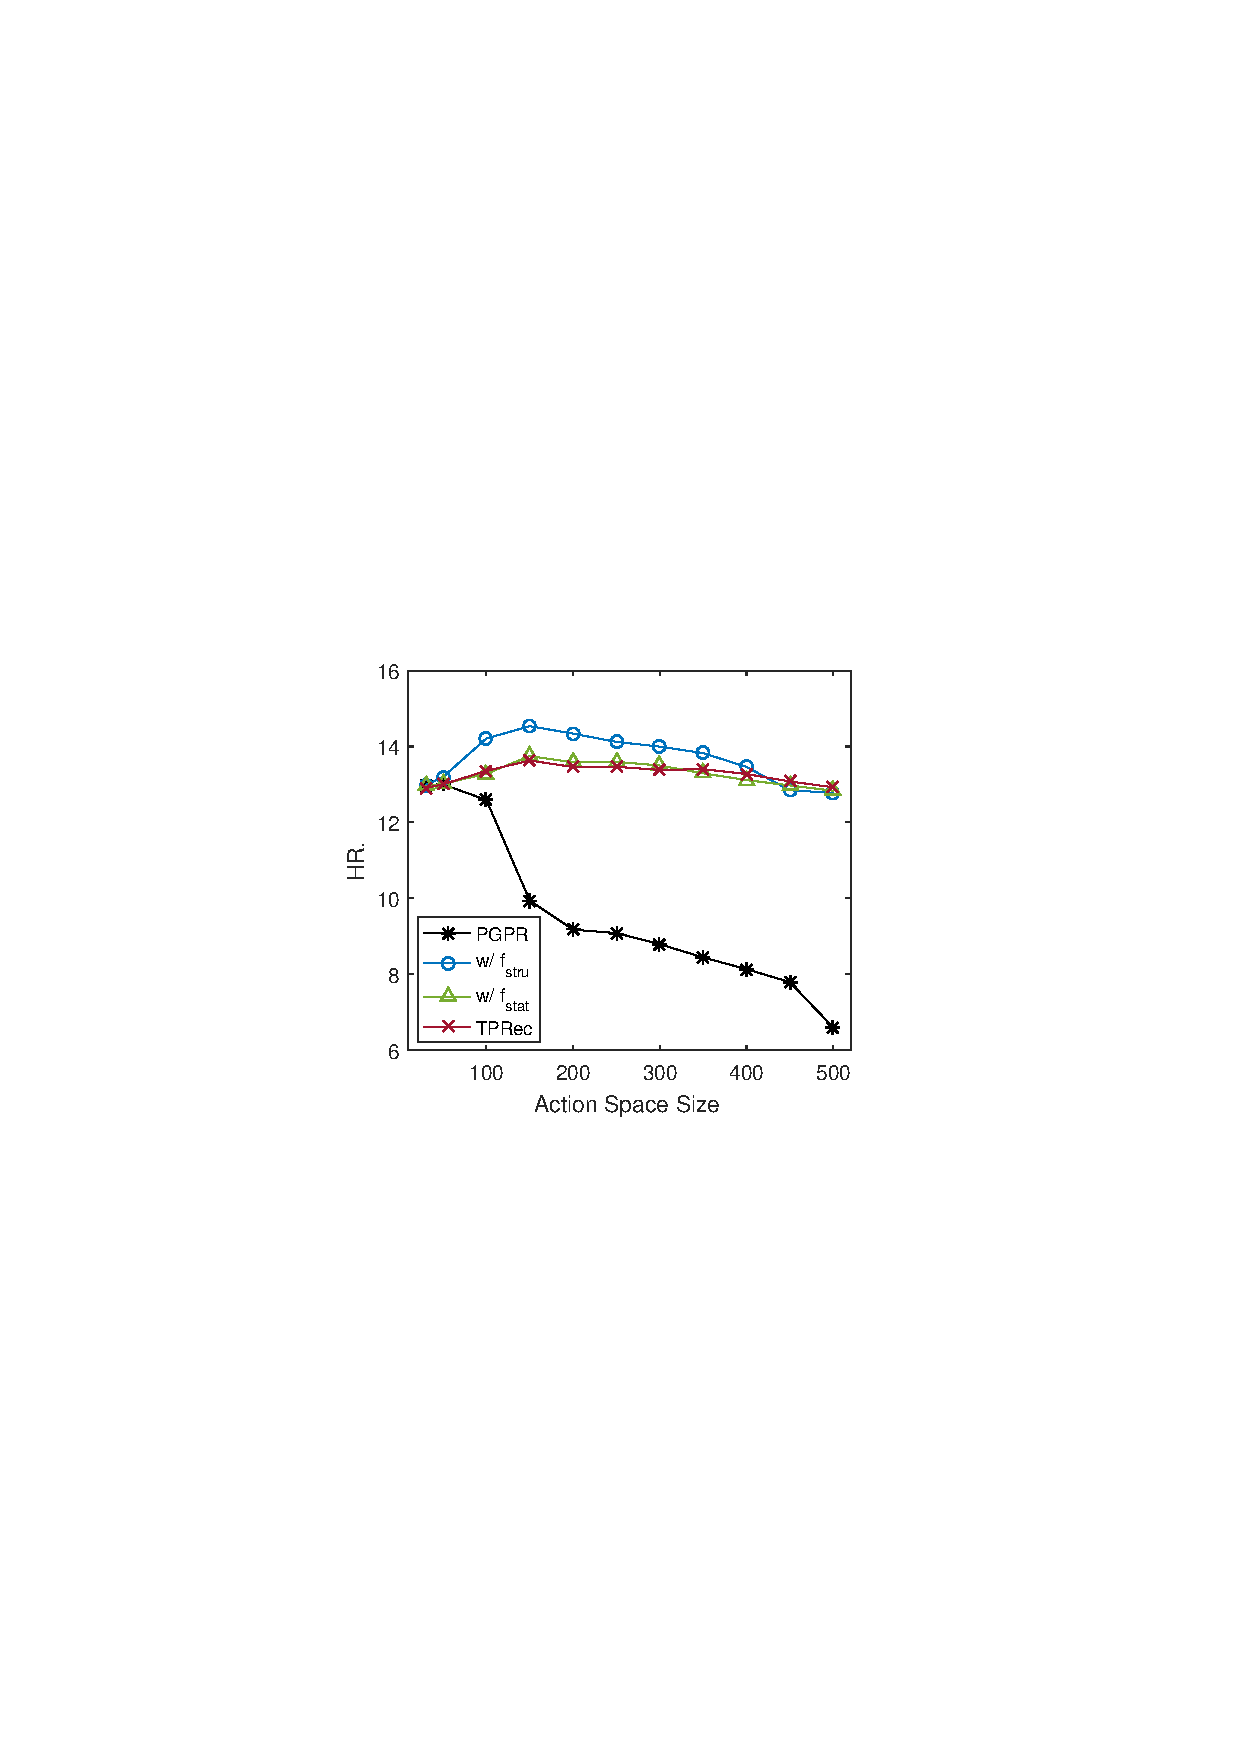
\includegraphics[width=1\textwidth]{chart/cell_hr.pdf}
		\end{minipage}
	}
	\subfloat[Precision (Cell).]{
		\begin{minipage}[t]{0.25\textwidth}
			\centering
			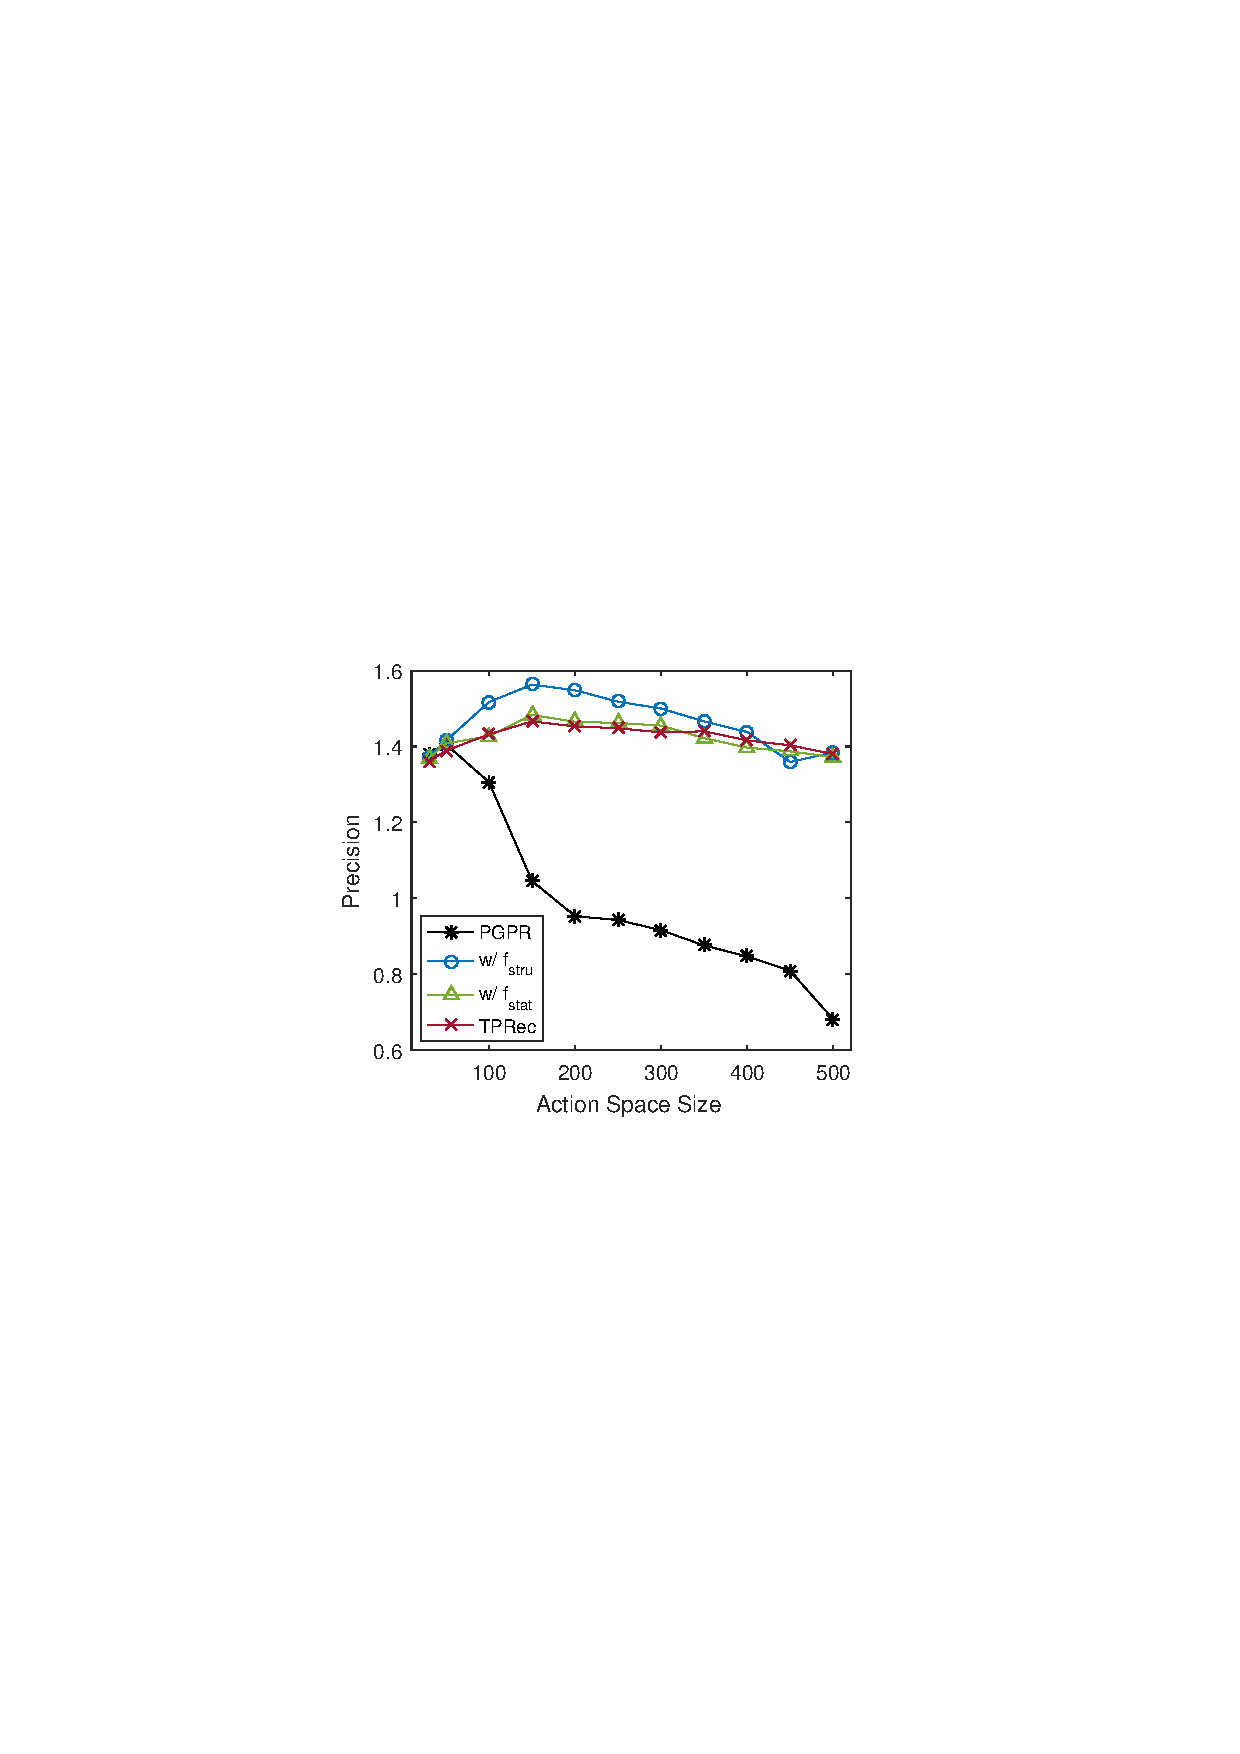
\includegraphics[width=1\textwidth]{chart/cell_prec.pdf}
		\end{minipage}
	}
	
	\subfloat[NDCG (Beauty).]{
		\begin{minipage}[t]{0.25\textwidth}
			\centering
			
\includegraphics[width=1\textwidth]{chart/beauty_ndcg.pdf}
		\end{minipage}
	}
		\subfloat[Recall (Beauty).]{
		\begin{minipage}[t]{0.25\textwidth}
			\centering
			
\includegraphics[width=1\textwidth]{chart/beauty_recall.pdf}
		\end{minipage}
	}
	\subfloat[HR (Beauty).]{
		\begin{minipage}[t]{0.25\textwidth}
			\centering
			
\includegraphics[width=1\textwidth]{chart/beauty_hr.pdf}
		\end{minipage}
	}
	\subfloat[Precision (Beauty).]{
		\begin{minipage}[t]{0.25\textwidth}
			\centering
			
\includegraphics[width=1\textwidth]{chart/beauty_prec.pdf}
		\end{minipage}
	}
\caption{ Effect of varying action space size $\epsilon$.
}
	\label{actionSpace}
\end{figure}



\subsubsection{\textbf{Effect of State History Length.}}
Figure \ref{stateHistory} presents the performance of four compared methods with different State History Length $k'$ in range $\{0,1,2\}$. We make the following observations: (1) with few exceptions, our \tkgrec\ consistently outperforms PGPR. (2) For all methods, the versions with encoding 1-step or 2-step history consistently outperform those without encoding history. This result validates the effectiveness of exploiting historical states to learn policy. But, we observe that encoding 2-step history may not be superior over 1-step. Too long history will bring some irrelevant information or even noises, which deteriorates recommendation performance.   
 
% We make the following two observations: (1) With few exceptions, all three versions of \tkgrec\ consistently outperform PGPR, demonstrating the effectiveness of exploiting temporal information. (2) Generally speaking, the performance of all the methods drops as $\epsilon$ increases. The reason is that a larger action space would increase the risk of retrieving irrelevant paths. Nonetheless, our \tkgrec\ drops relatively mildly. This result implies our \tkgrec\ is more robust to the $\epsilon$ as it is more powerful to identify high-quality paths with leveraging temporal information. Also, we find the smallest $\epsilon$ may not bring optimal performance. It can be seen from the inferior performance of some methods with $\epsilon=100$ comparing with $\epsilon=150$. It may be caused by the missing of the target paths in the action space when $\epsilon$ is too small.
%
%
%In this experiment, we study how the length of state history influences the recommendation performance of our method.
%Recall that in Section \ref{secMDP}, we define $k'$-step history to encode the combination of entities and relations in the past $k'$ step.
%Since we set the maximum path length to $k=3$, thus, our state history length $k'$ is set to [0, 1, 2]. Intuitively, a larger history length will contain more path reasoning information for promoting recommendation.
%
%Figure \ref{stateHistory} illustrates our performance w.r.t. different state history length on three datasets. As shown in Figure \ref{stateHistory}, the performance of using 1-step history and 2-step history further outperforms the general 0-step history.
%This improvement demonstrate that the state representation with history could help the RL agent to learn a good policy with sufficient information. What's more, the performance of 2-step history was not improved compared with 1-step history. The reason may be that too much historical information introduces additional noise and fails to provide effective information to guide the RL agent.


% 能够捕获更远的信息, 但是太远了诱惑噪音.

% 后面就讲啊, 什么更短更没有信息啊, 更长引入更多噪音啊, 所以设为1 啊.

\begin{figure}[]
	\centering
	\subfloat[NDCG (Clothing).]{
		\begin{minipage}[t]{0.25\textwidth}
			\centering
			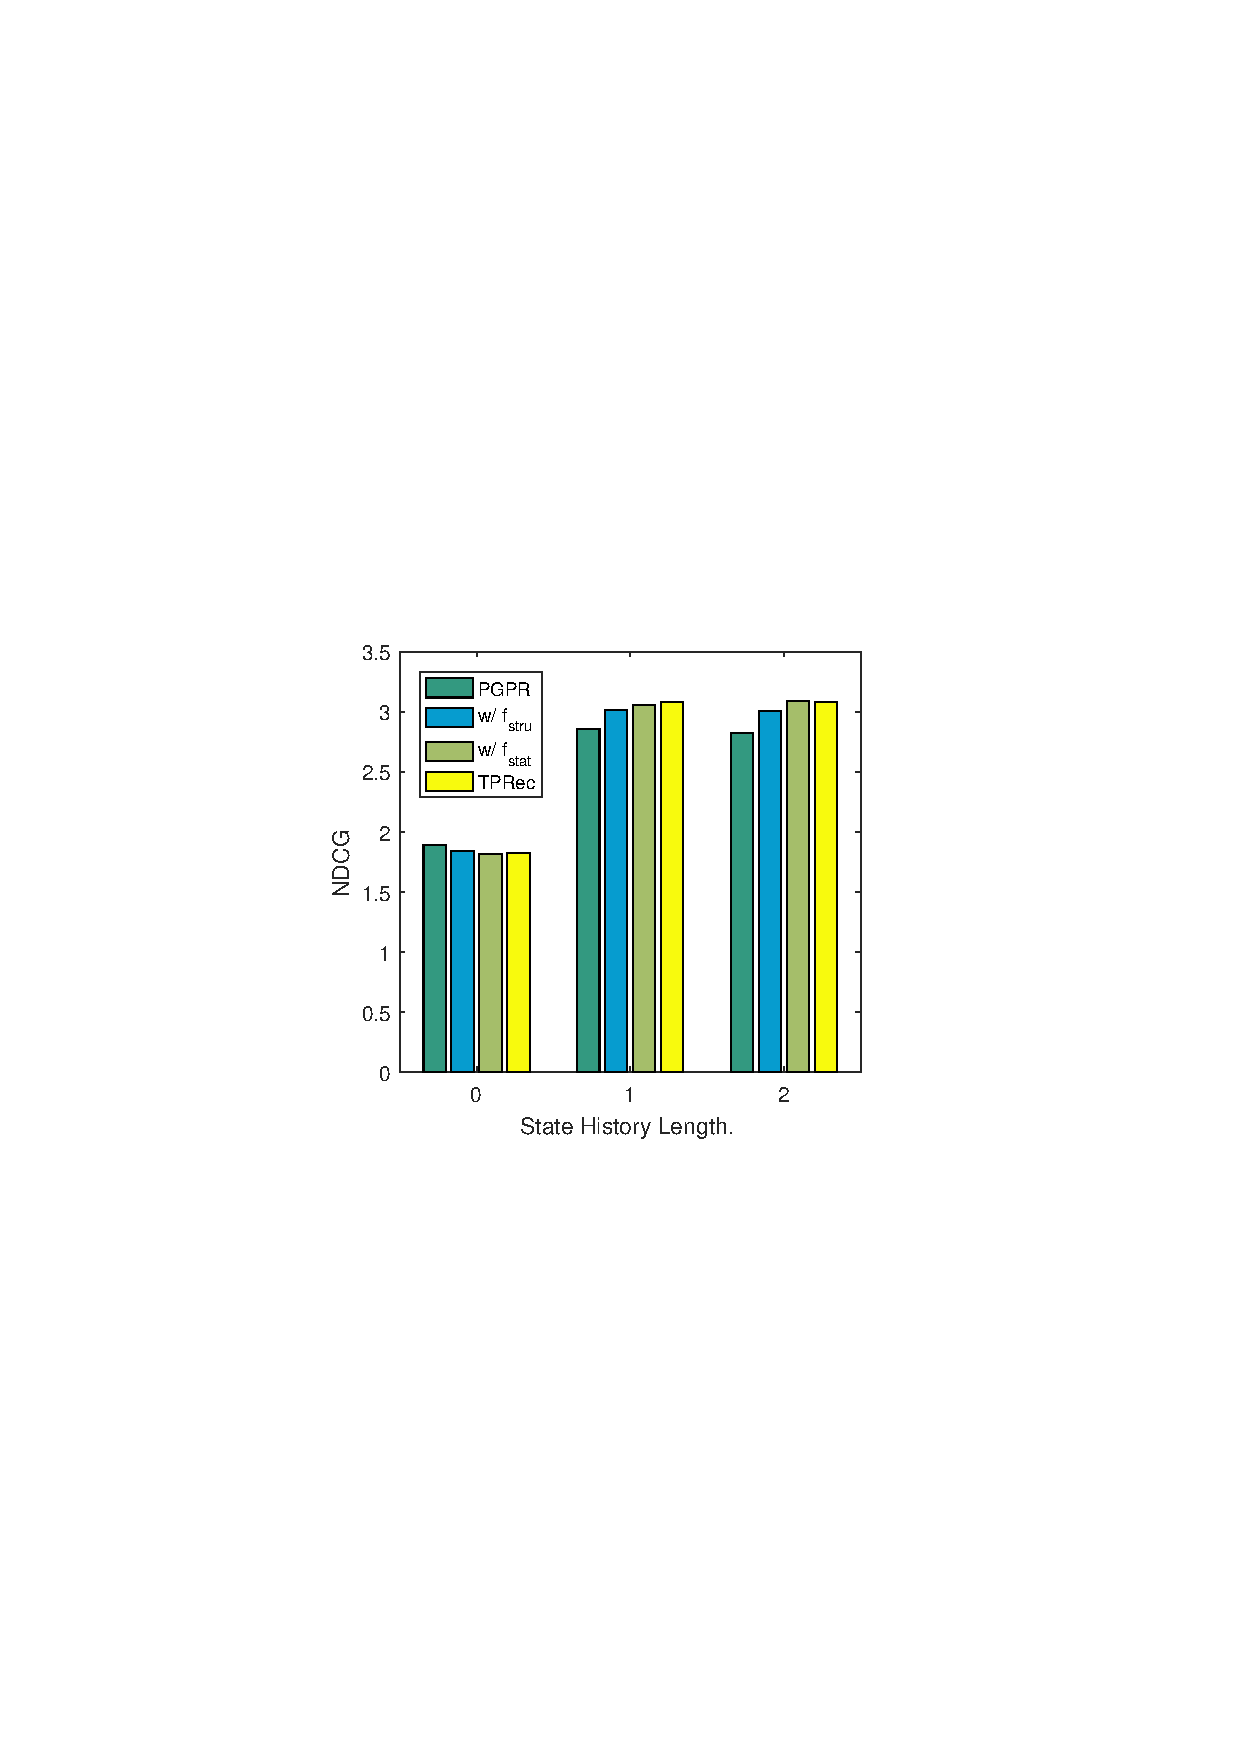
\includegraphics[width=1\textwidth]{chart/cloth_s_ndcg.pdf}
		\end{minipage}
	}
	\subfloat[Recall (Clothing).]{
		\begin{minipage}[t]{0.25\textwidth}
			\centering
			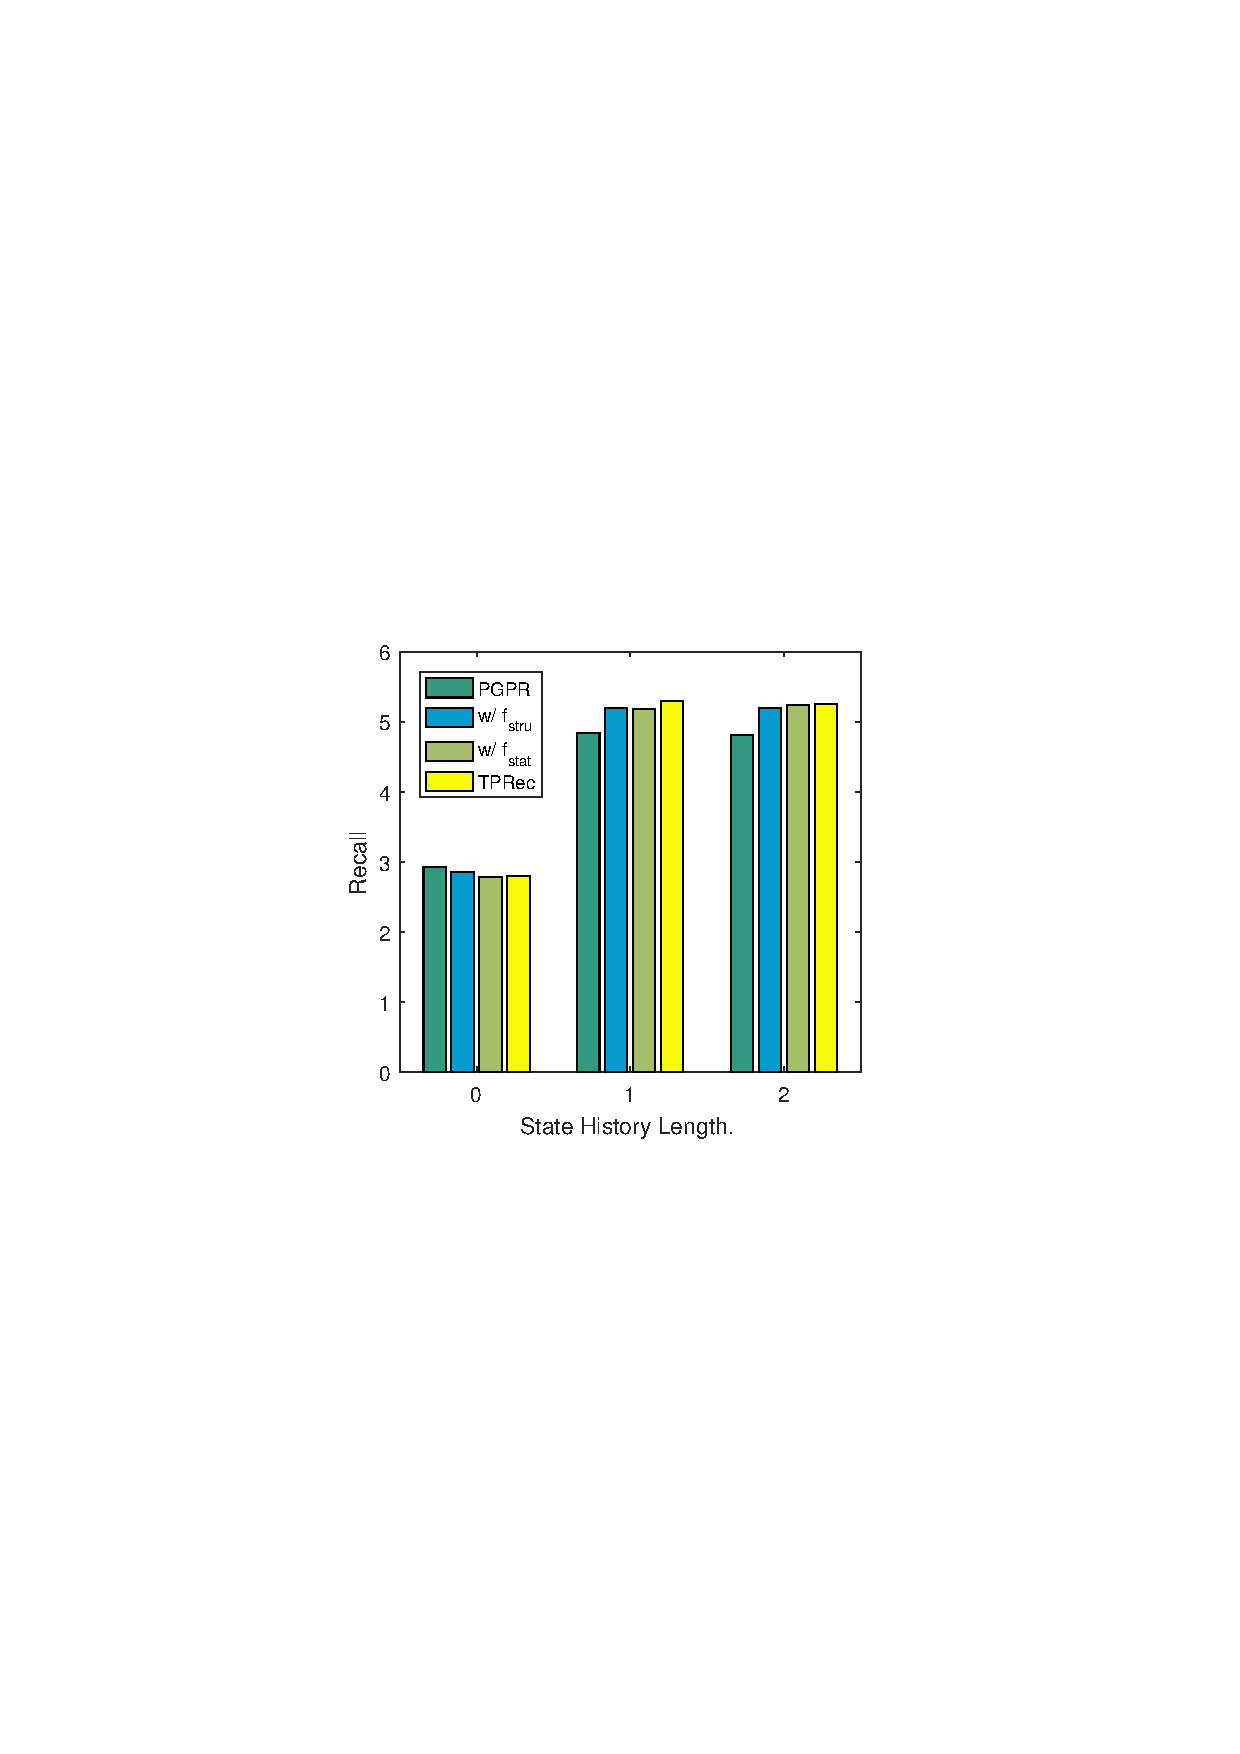
\includegraphics[width=1\textwidth]{chart/cloth_s_recall.pdf}
		\end{minipage}
	}
	\subfloat[HR (Clothing).]{
		\begin{minipage}[t]{0.25\textwidth}
			\centering
			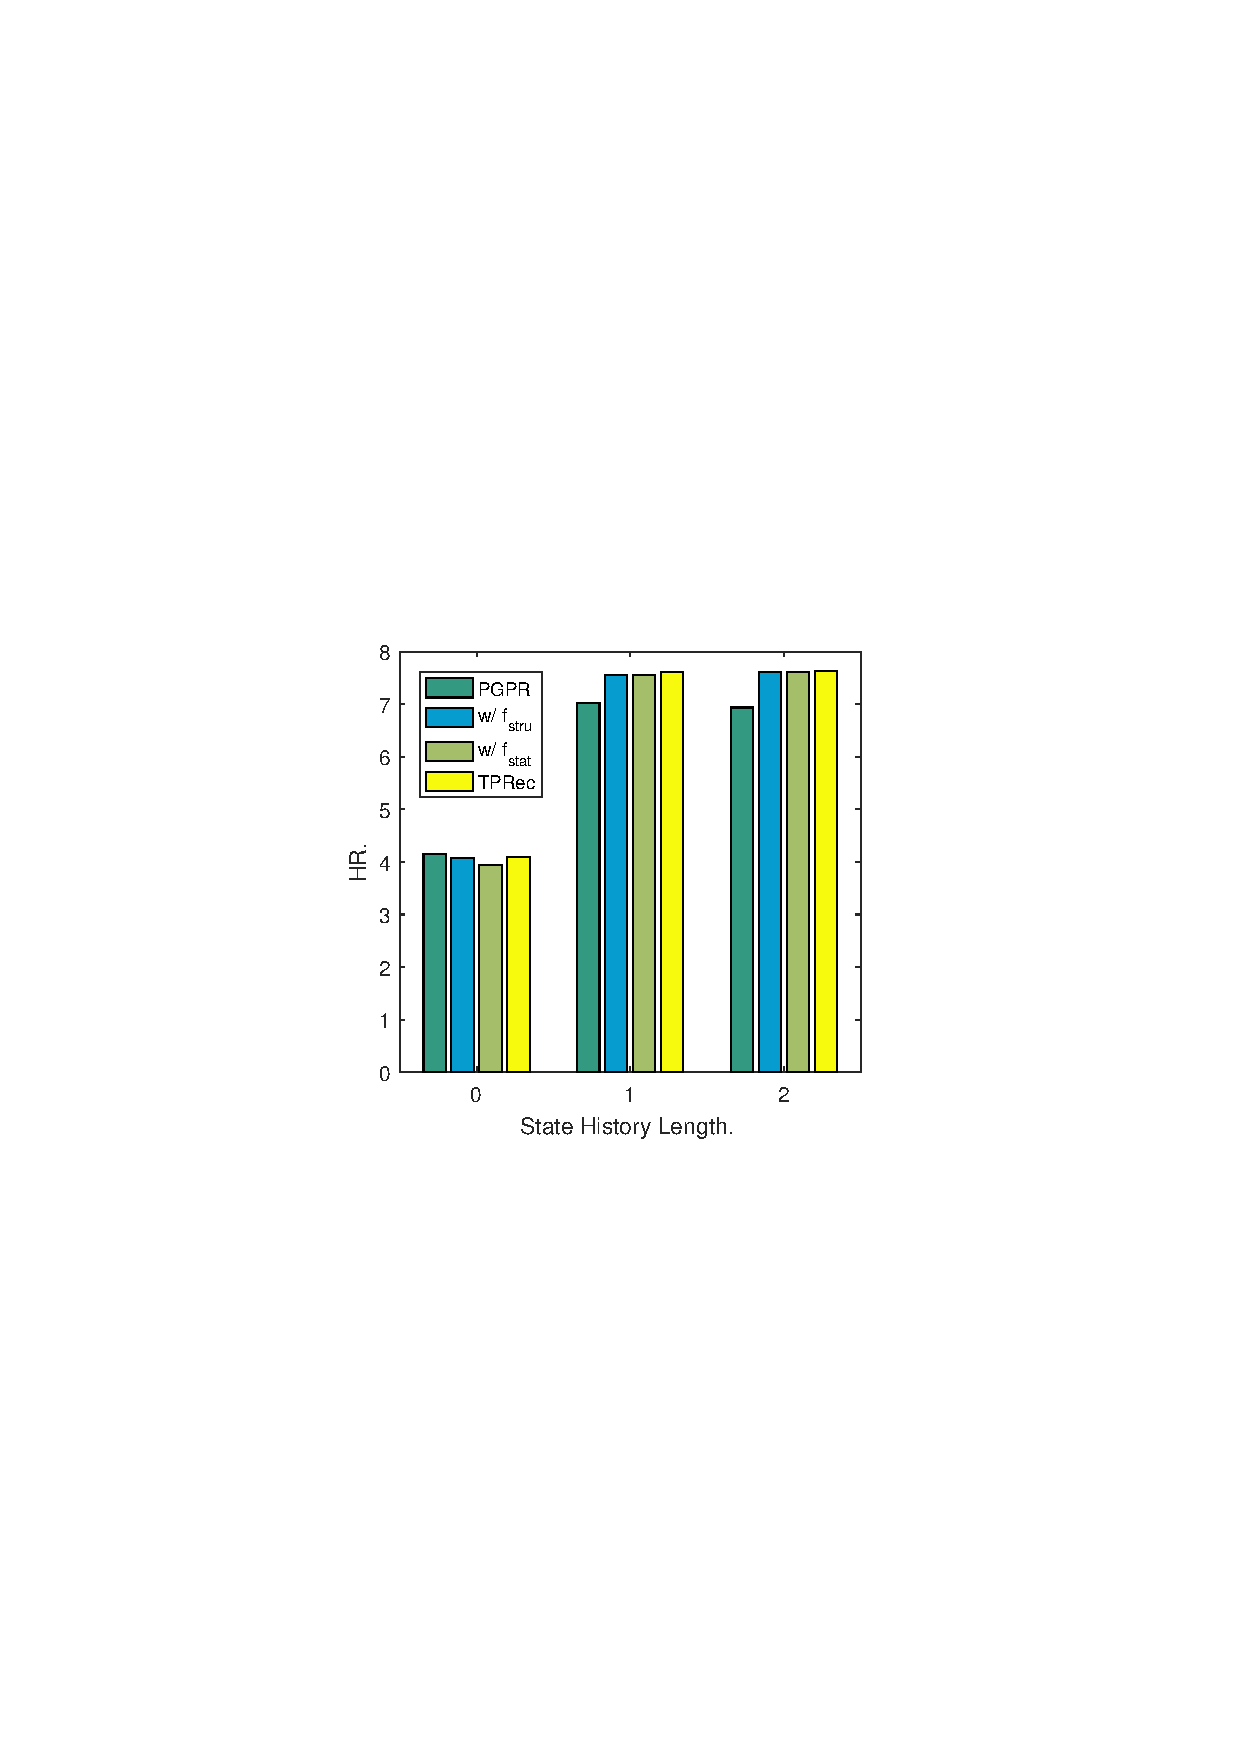
\includegraphics[width=1\textwidth]{chart/cloth_s_hr.pdf}
		\end{minipage}
	}
	\subfloat[Precision (Clothing).]{
		\begin{minipage}[t]{0.25\textwidth}
			\centering
			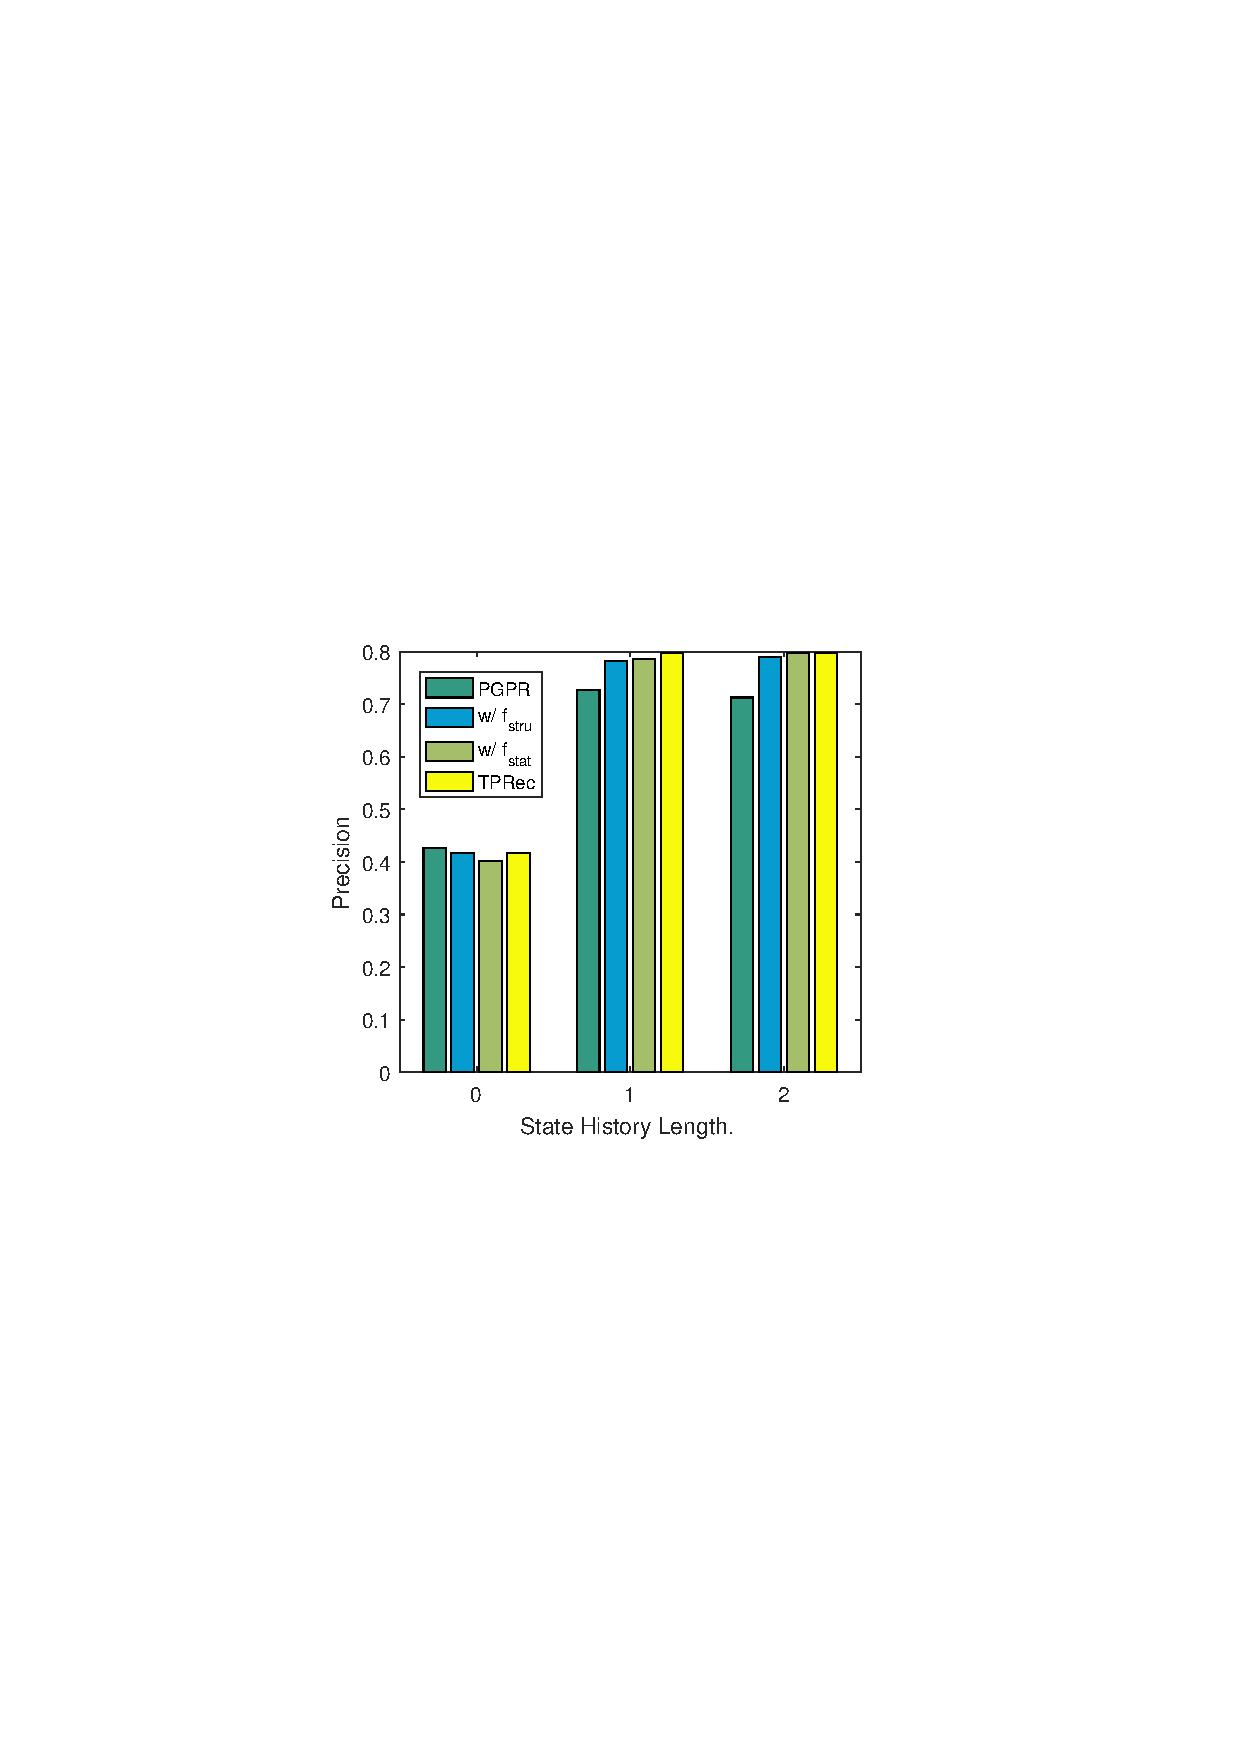
\includegraphics[width=1\textwidth]{chart/cloth_s_prec.pdf}
		\end{minipage}
	}
	
	\subfloat[NDCG (Clothing).]{
		\begin{minipage}[t]{0.25\textwidth}
			\centering
			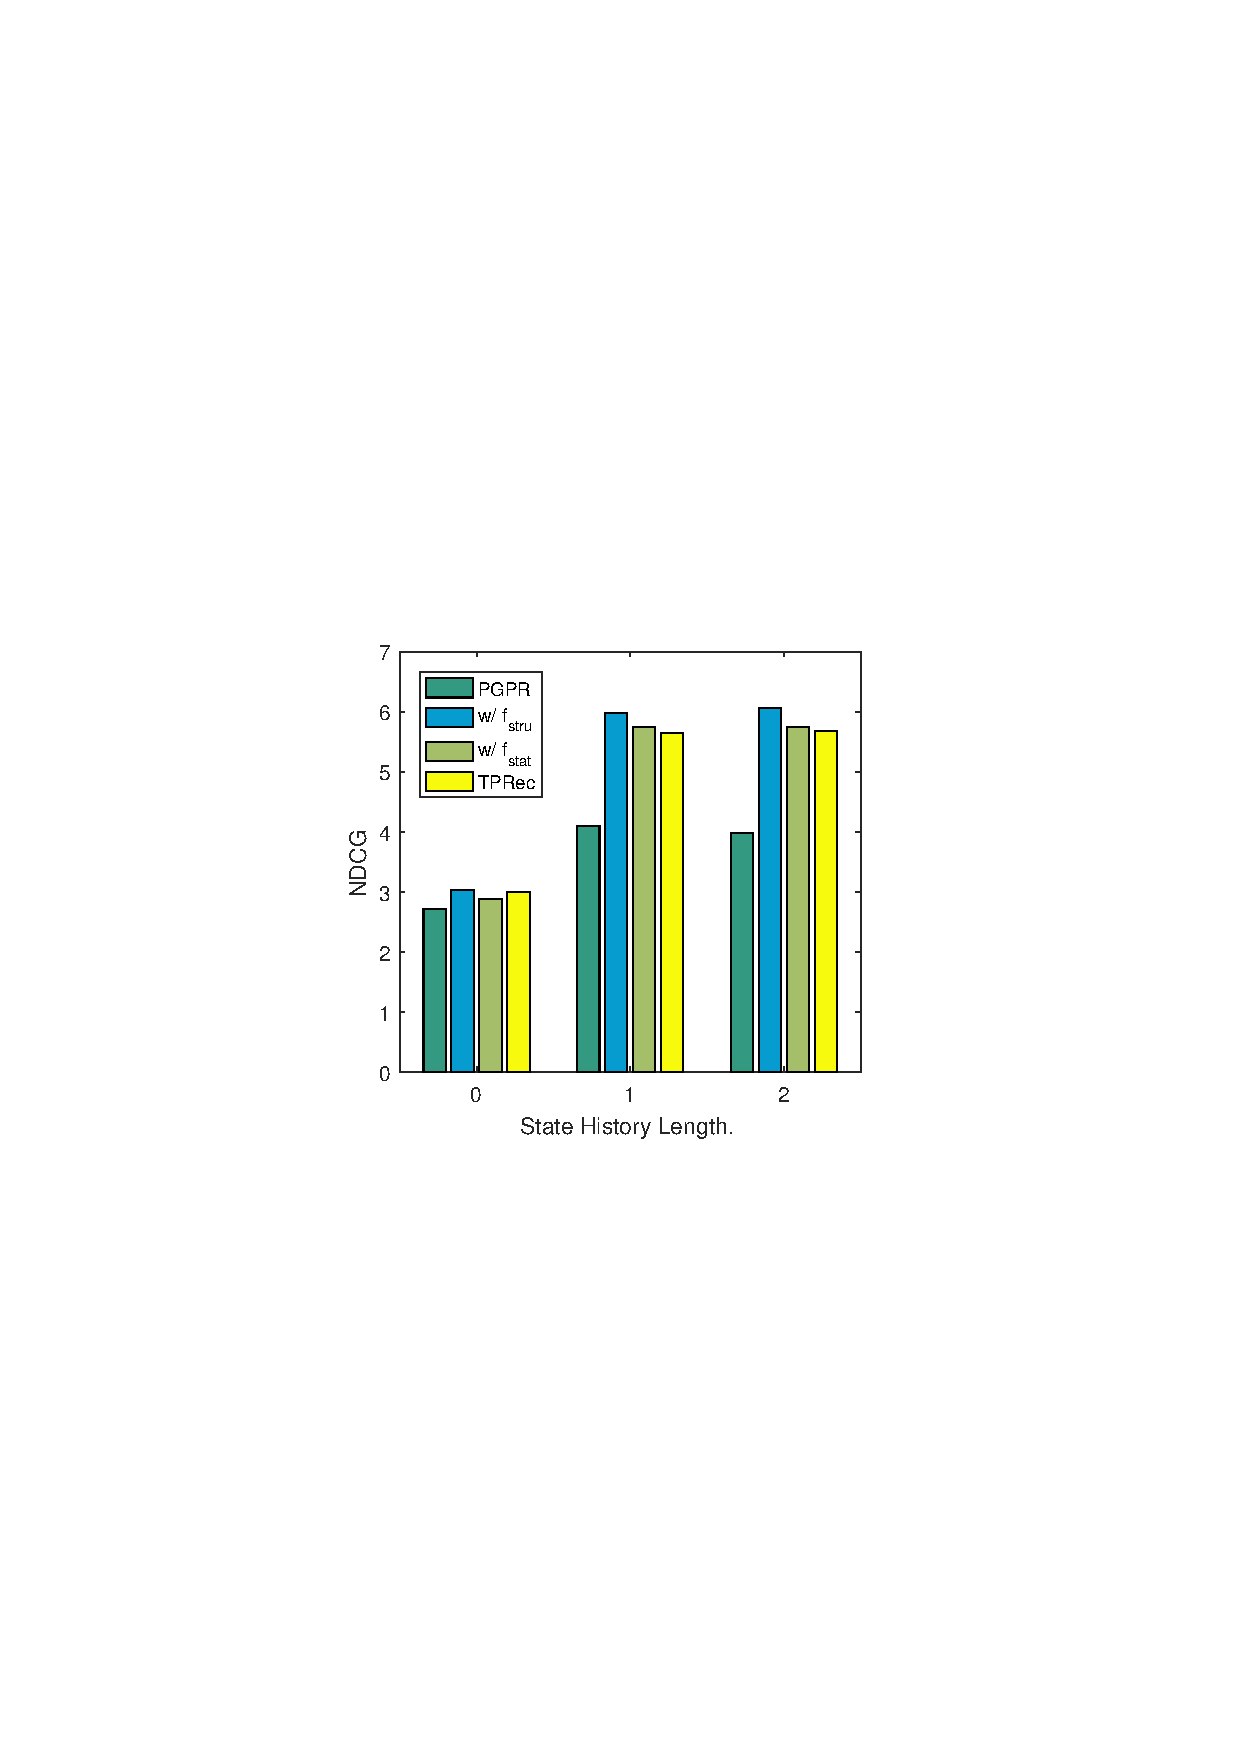
\includegraphics[width=1\textwidth]{chart/cell_s_ndcg.pdf}
		\end{minipage}
	}
	\subfloat[Recall (Cell).]{
		\begin{minipage}[t]{0.25\textwidth}
			\centering
			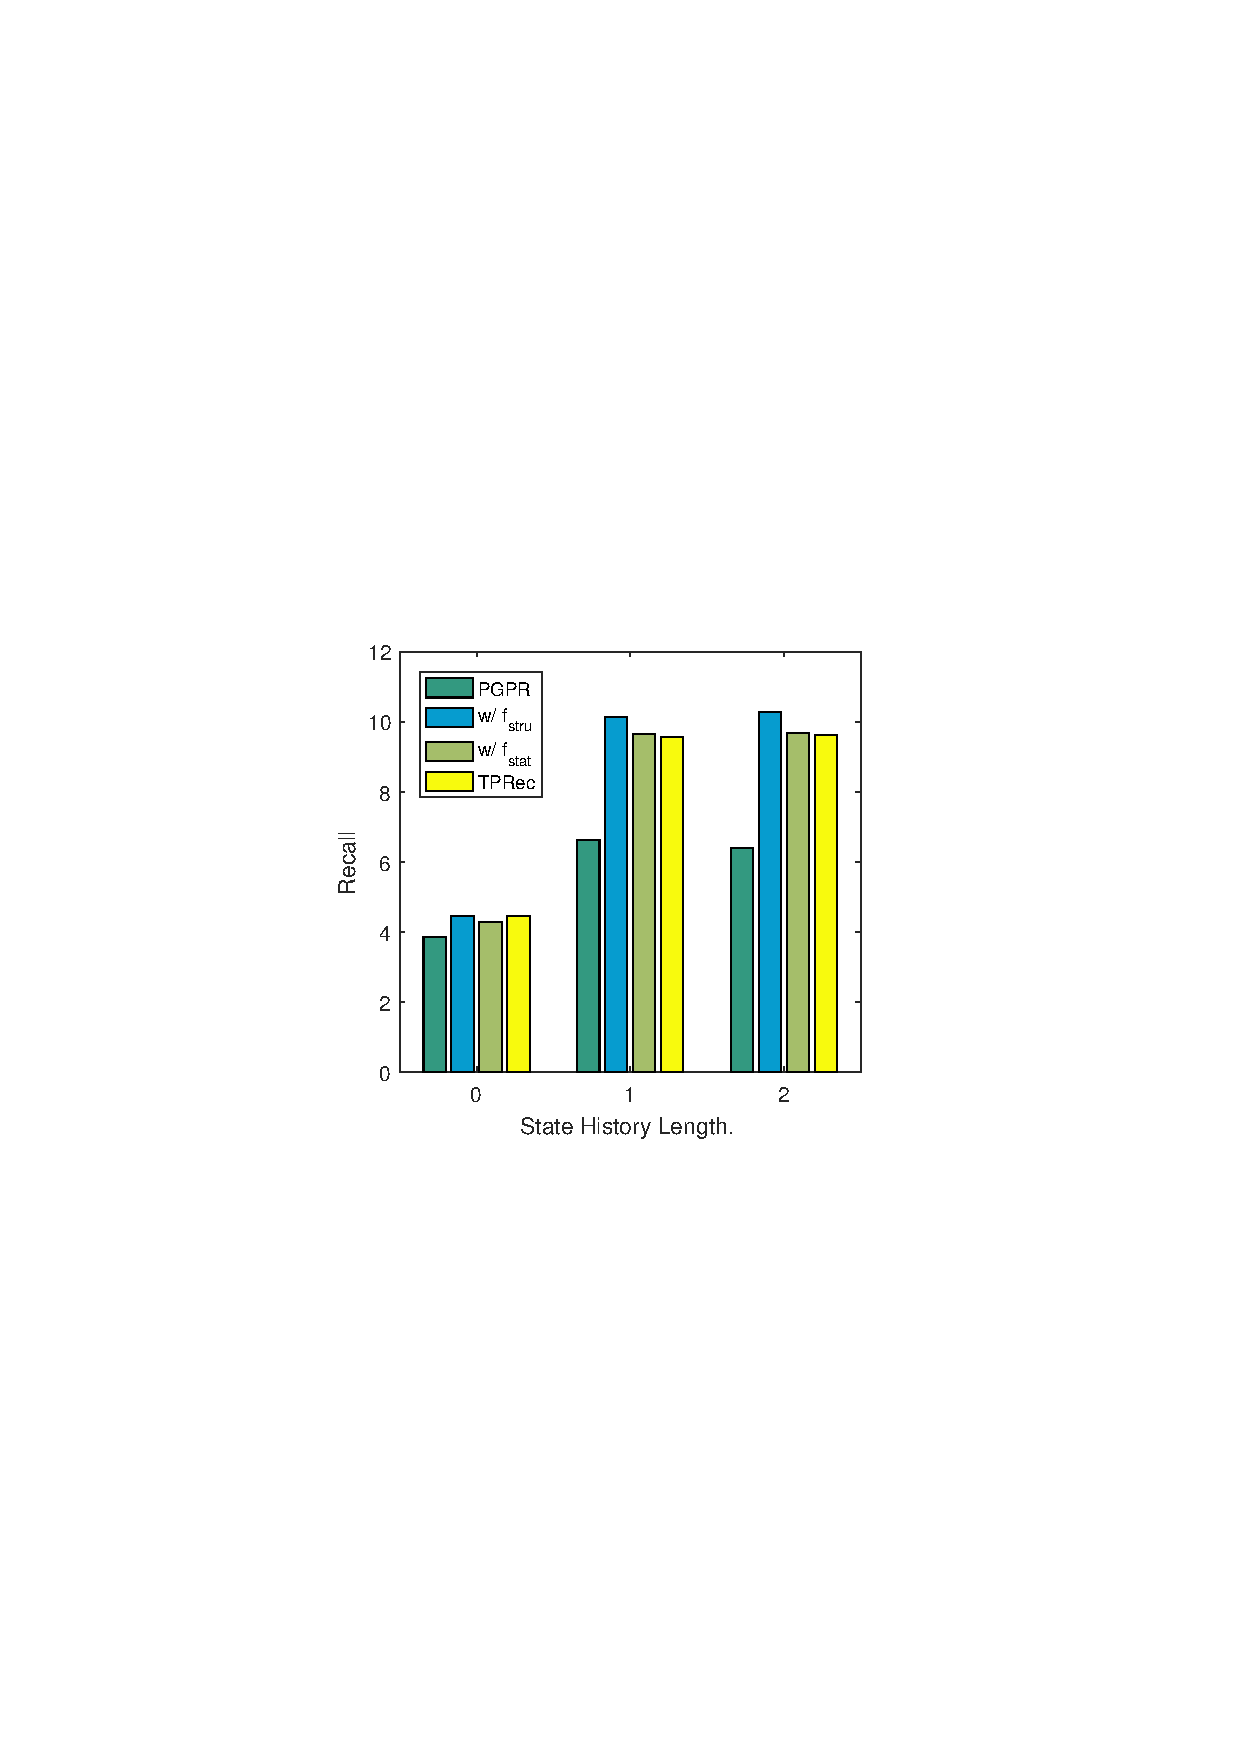
\includegraphics[width=1\textwidth]{chart/cell_s_recall.pdf}
		\end{minipage}
	}
	\subfloat[HR (Cell).]{
		\begin{minipage}[t]{0.25\textwidth}
			\centering
			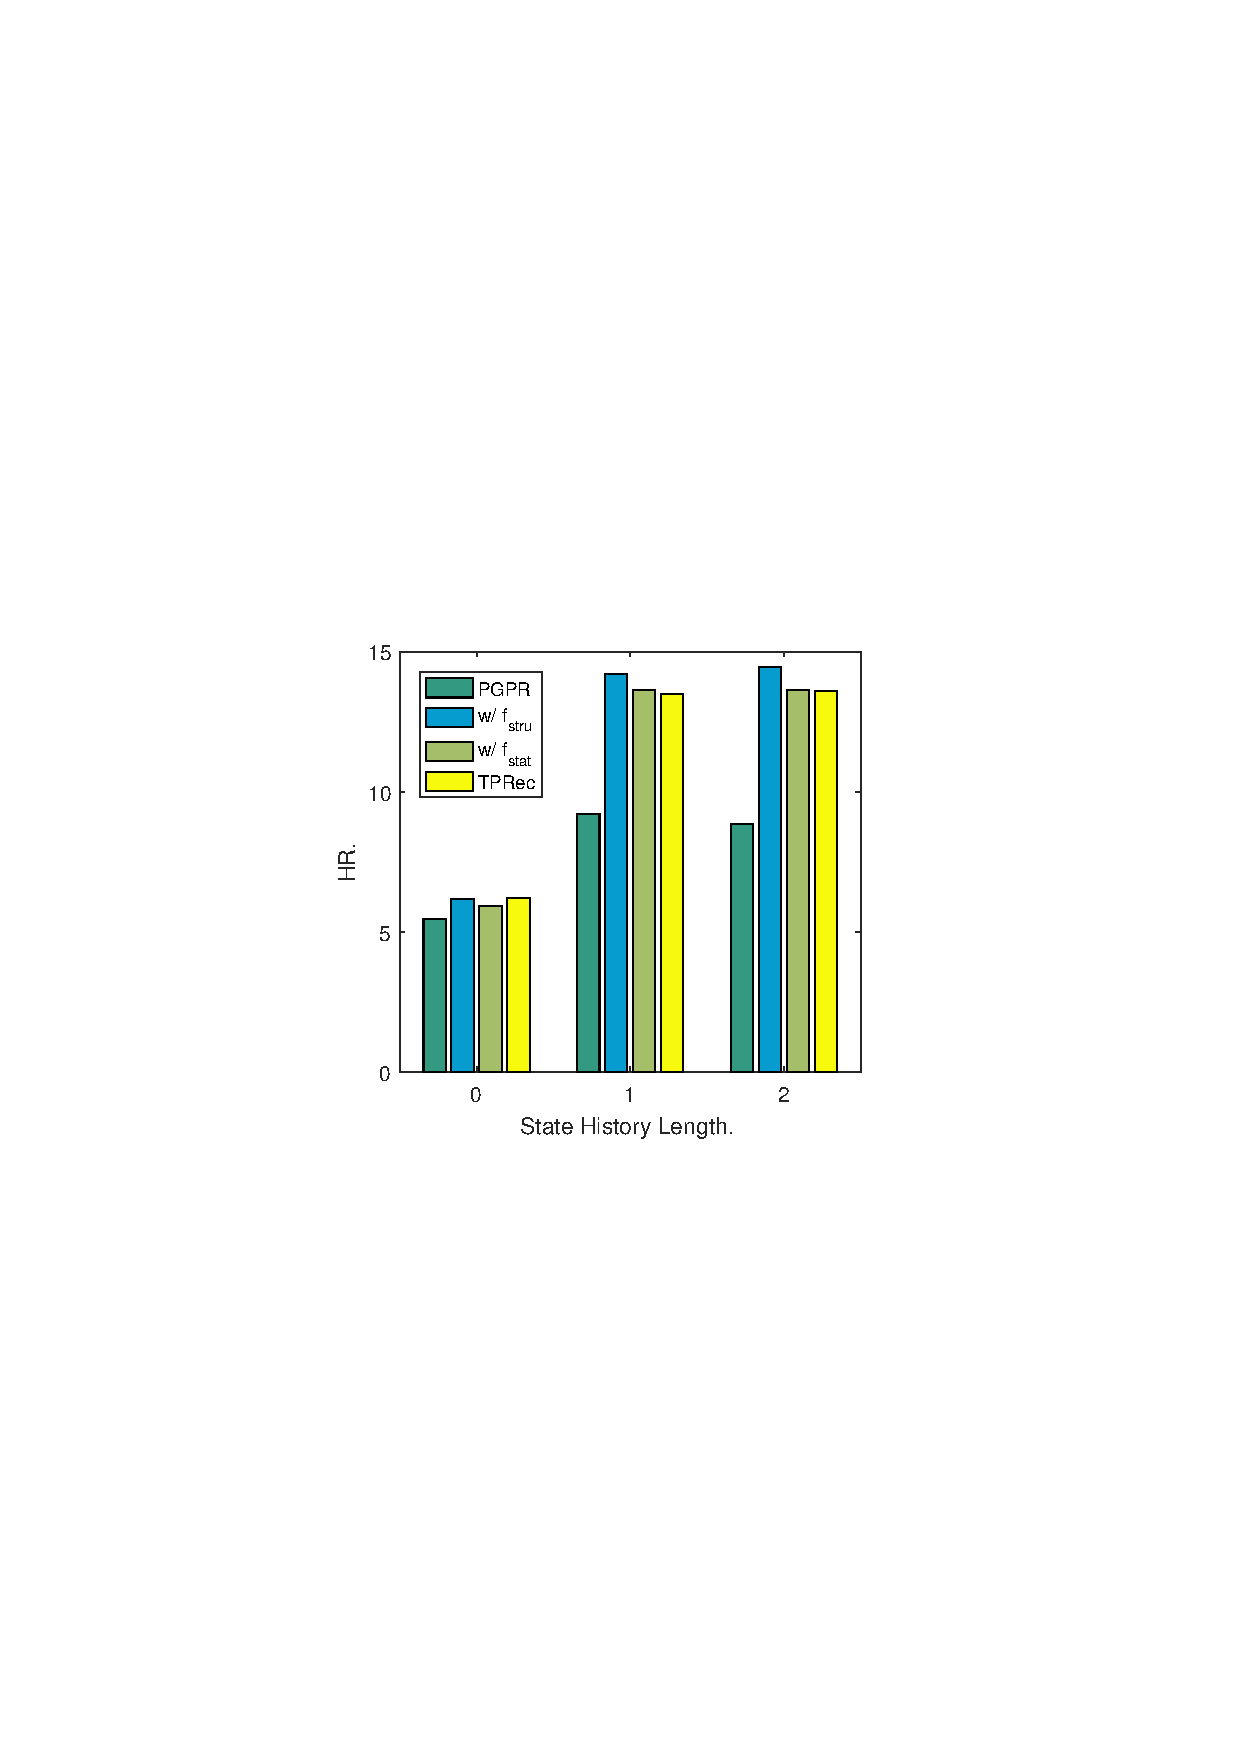
\includegraphics[width=1\textwidth]{chart/cell_s_hr.pdf}
		\end{minipage}
	}
	\subfloat[Precision (Cell).]{
		\begin{minipage}[t]{0.25\textwidth}
			\centering
			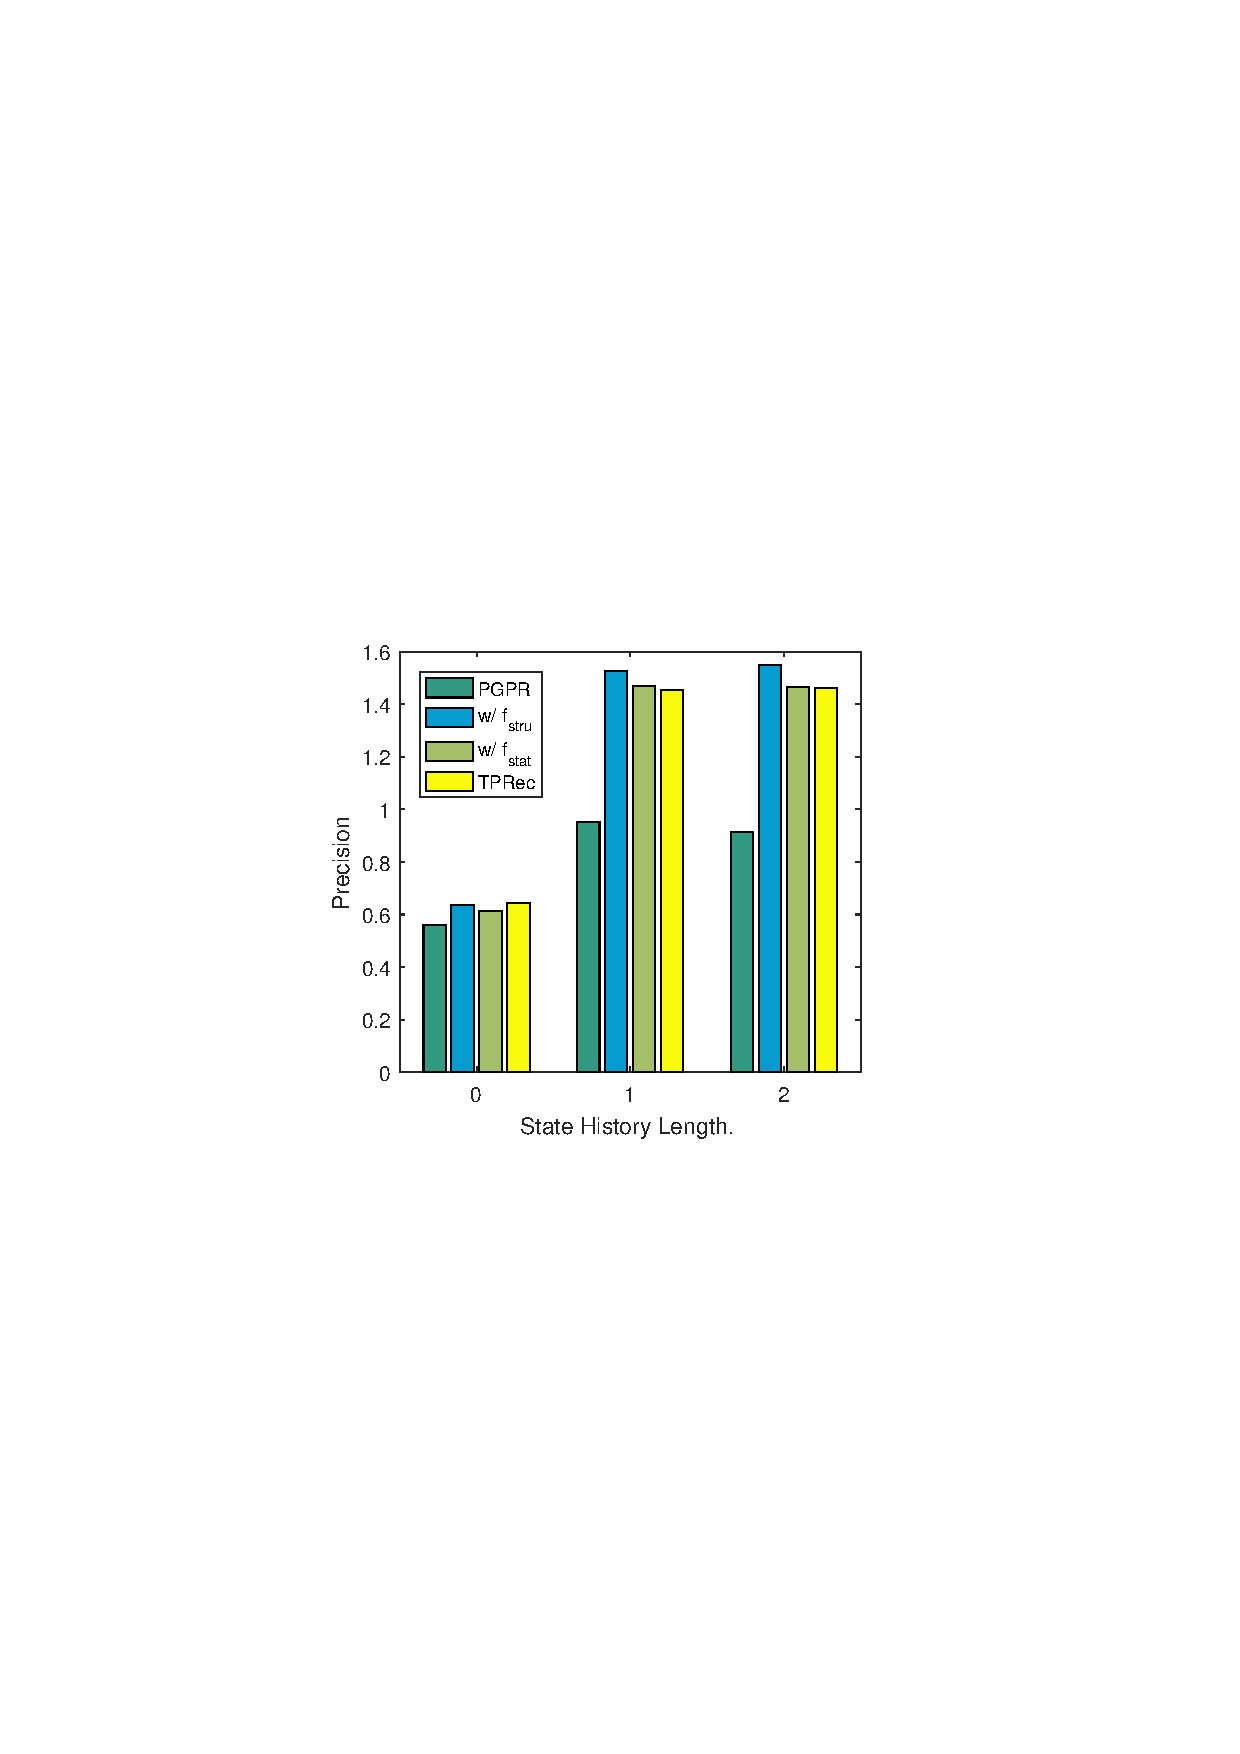
\includegraphics[width=1\textwidth]{chart/cell_s_prec.pdf}
		\end{minipage}
	}
	
	\subfloat[NDCG (Beauty).]{
		\begin{minipage}[t]{0.25\textwidth}
			\centering
			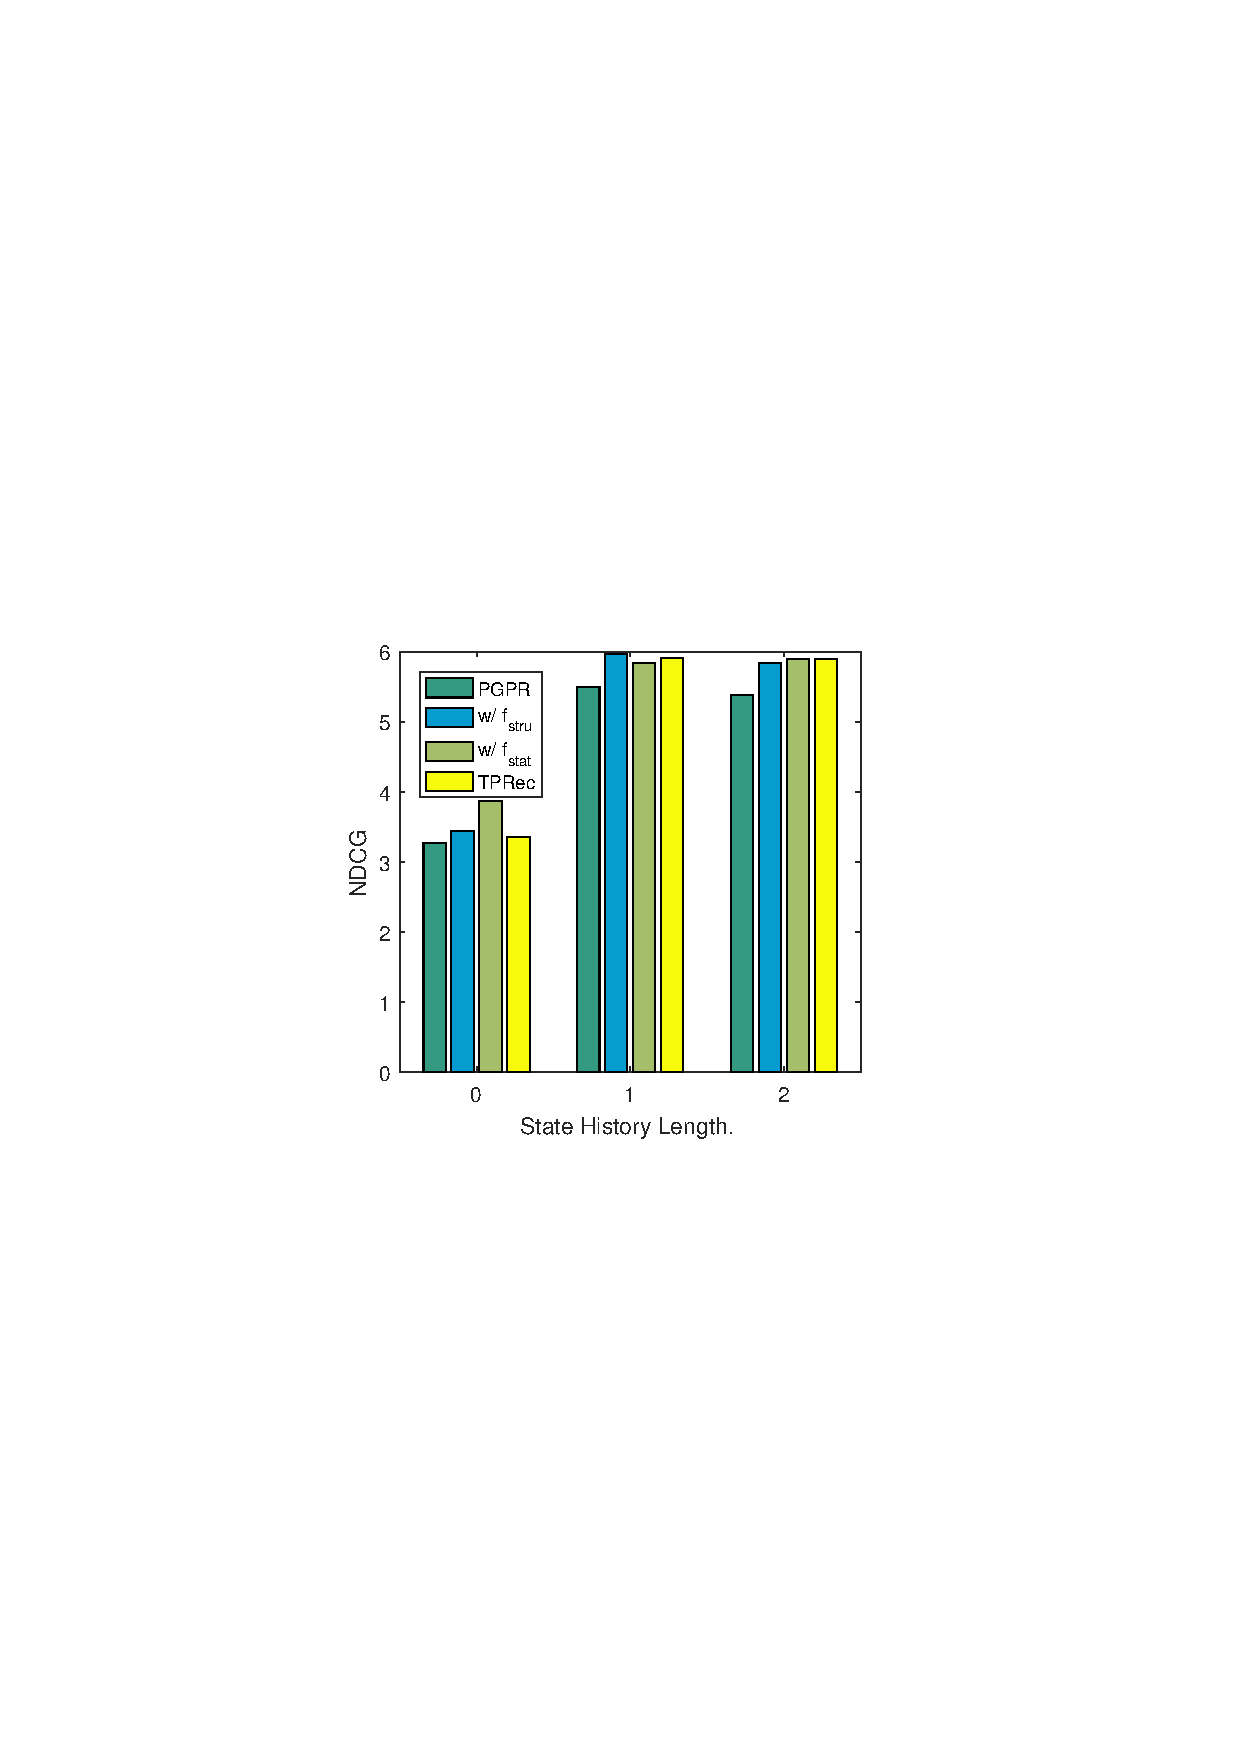
\includegraphics[width=1\textwidth]{chart/beauty_s_ndcg.pdf}
		\end{minipage}
	}
		\subfloat[Recall (Beauty).]{
		\begin{minipage}[t]{0.25\textwidth}
			\centering
			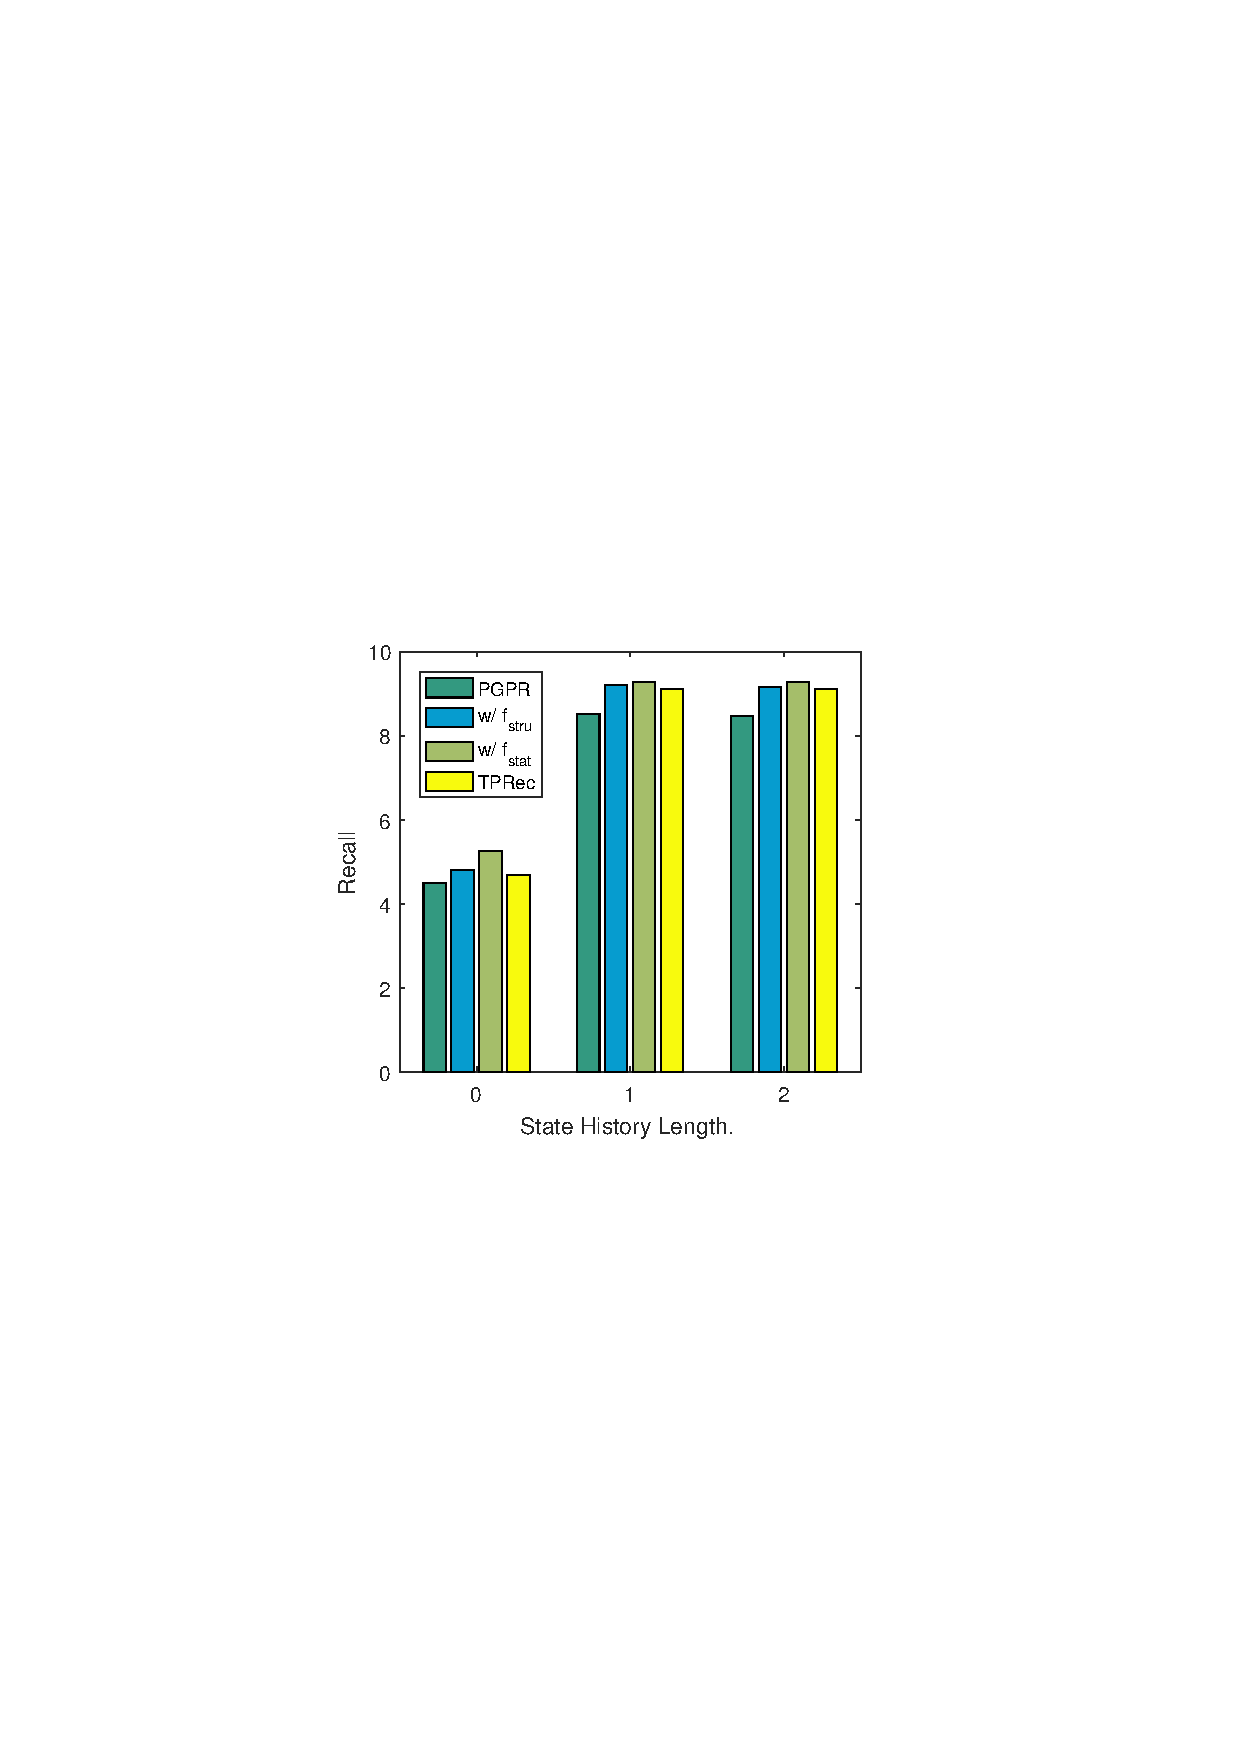
\includegraphics[width=1\textwidth]{chart/beauty_s_recall.pdf}
		\end{minipage}
	}
	\subfloat[HR (Beauty).]{
		\begin{minipage}[t]{0.25\textwidth}
			\centering
			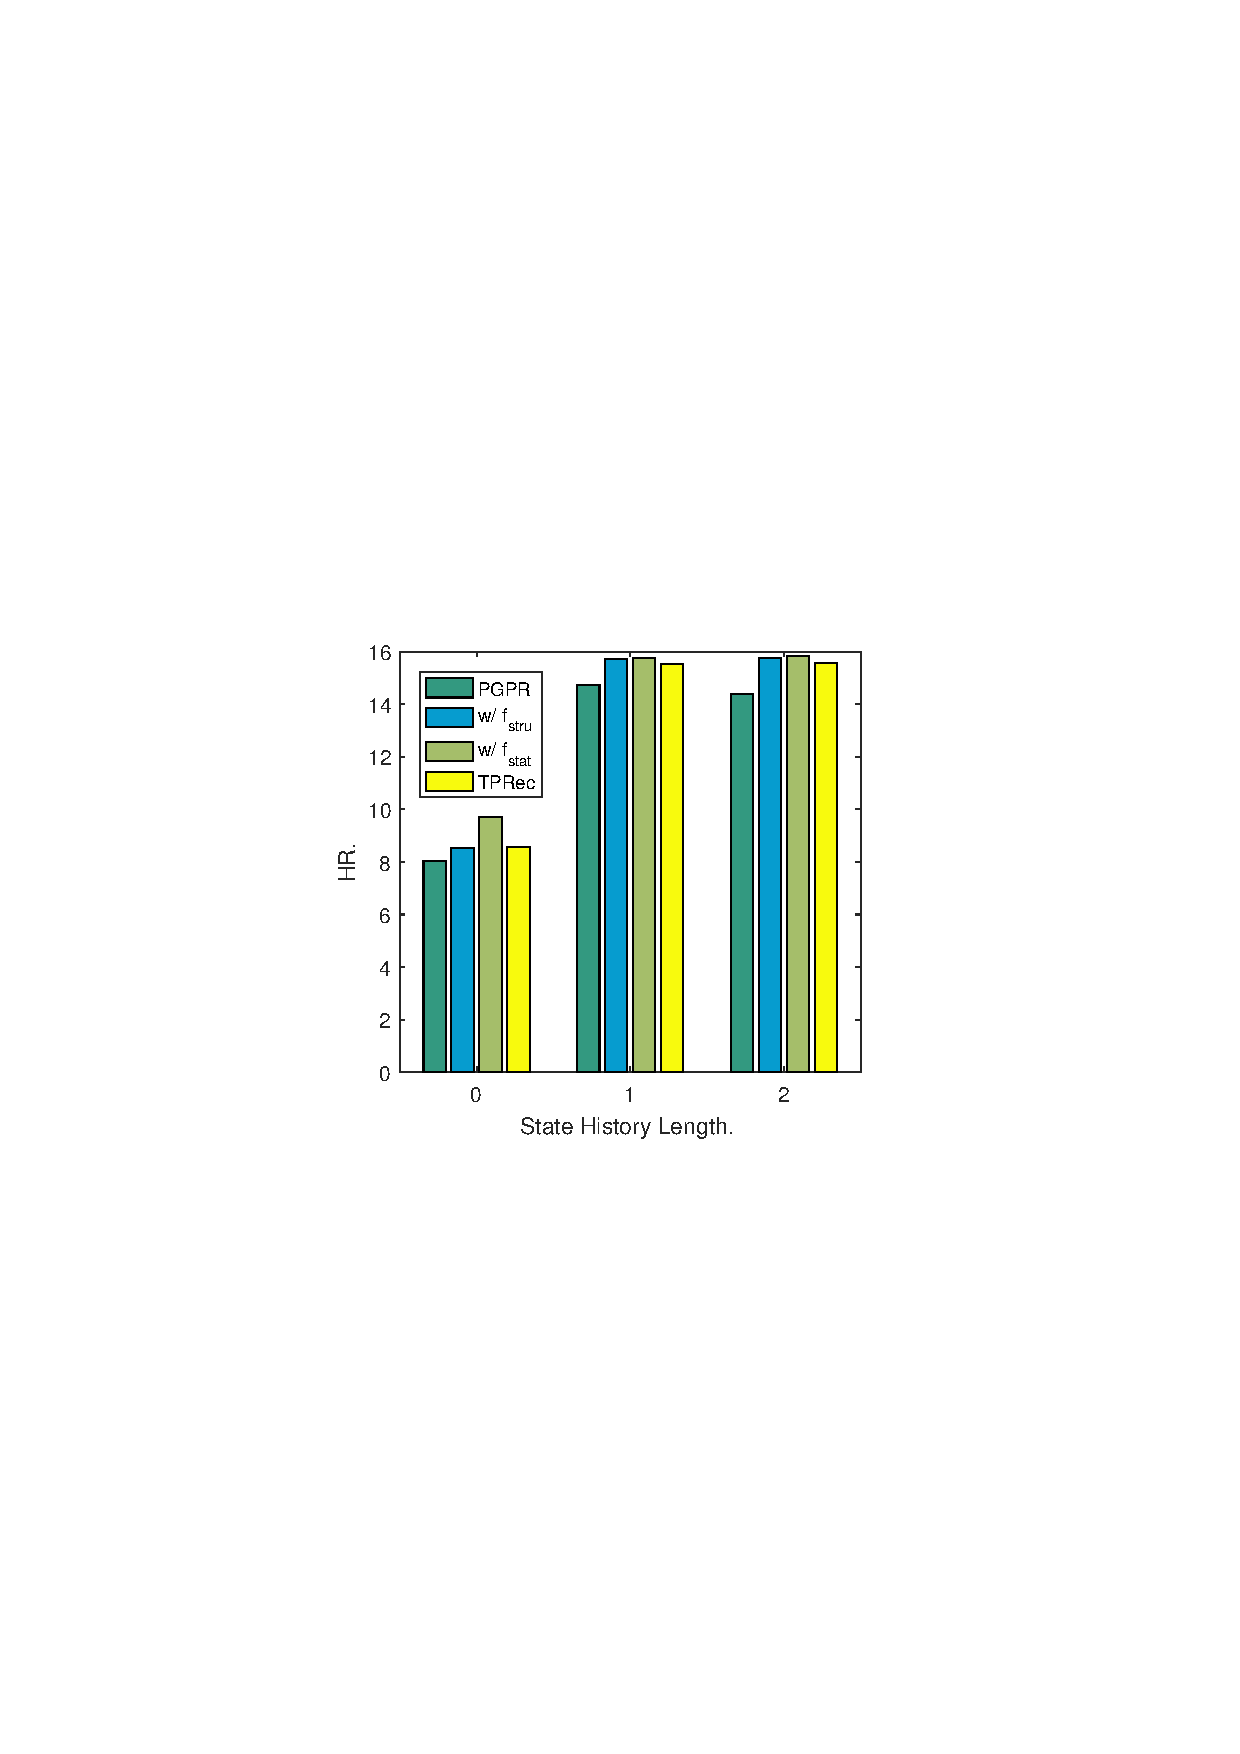
\includegraphics[width=1\textwidth]{chart/beauty_s_hr.pdf}
		\end{minipage}
	}
	\subfloat[Precision (Beauty).]{
		\begin{minipage}[t]{0.25\textwidth}
			\centering
			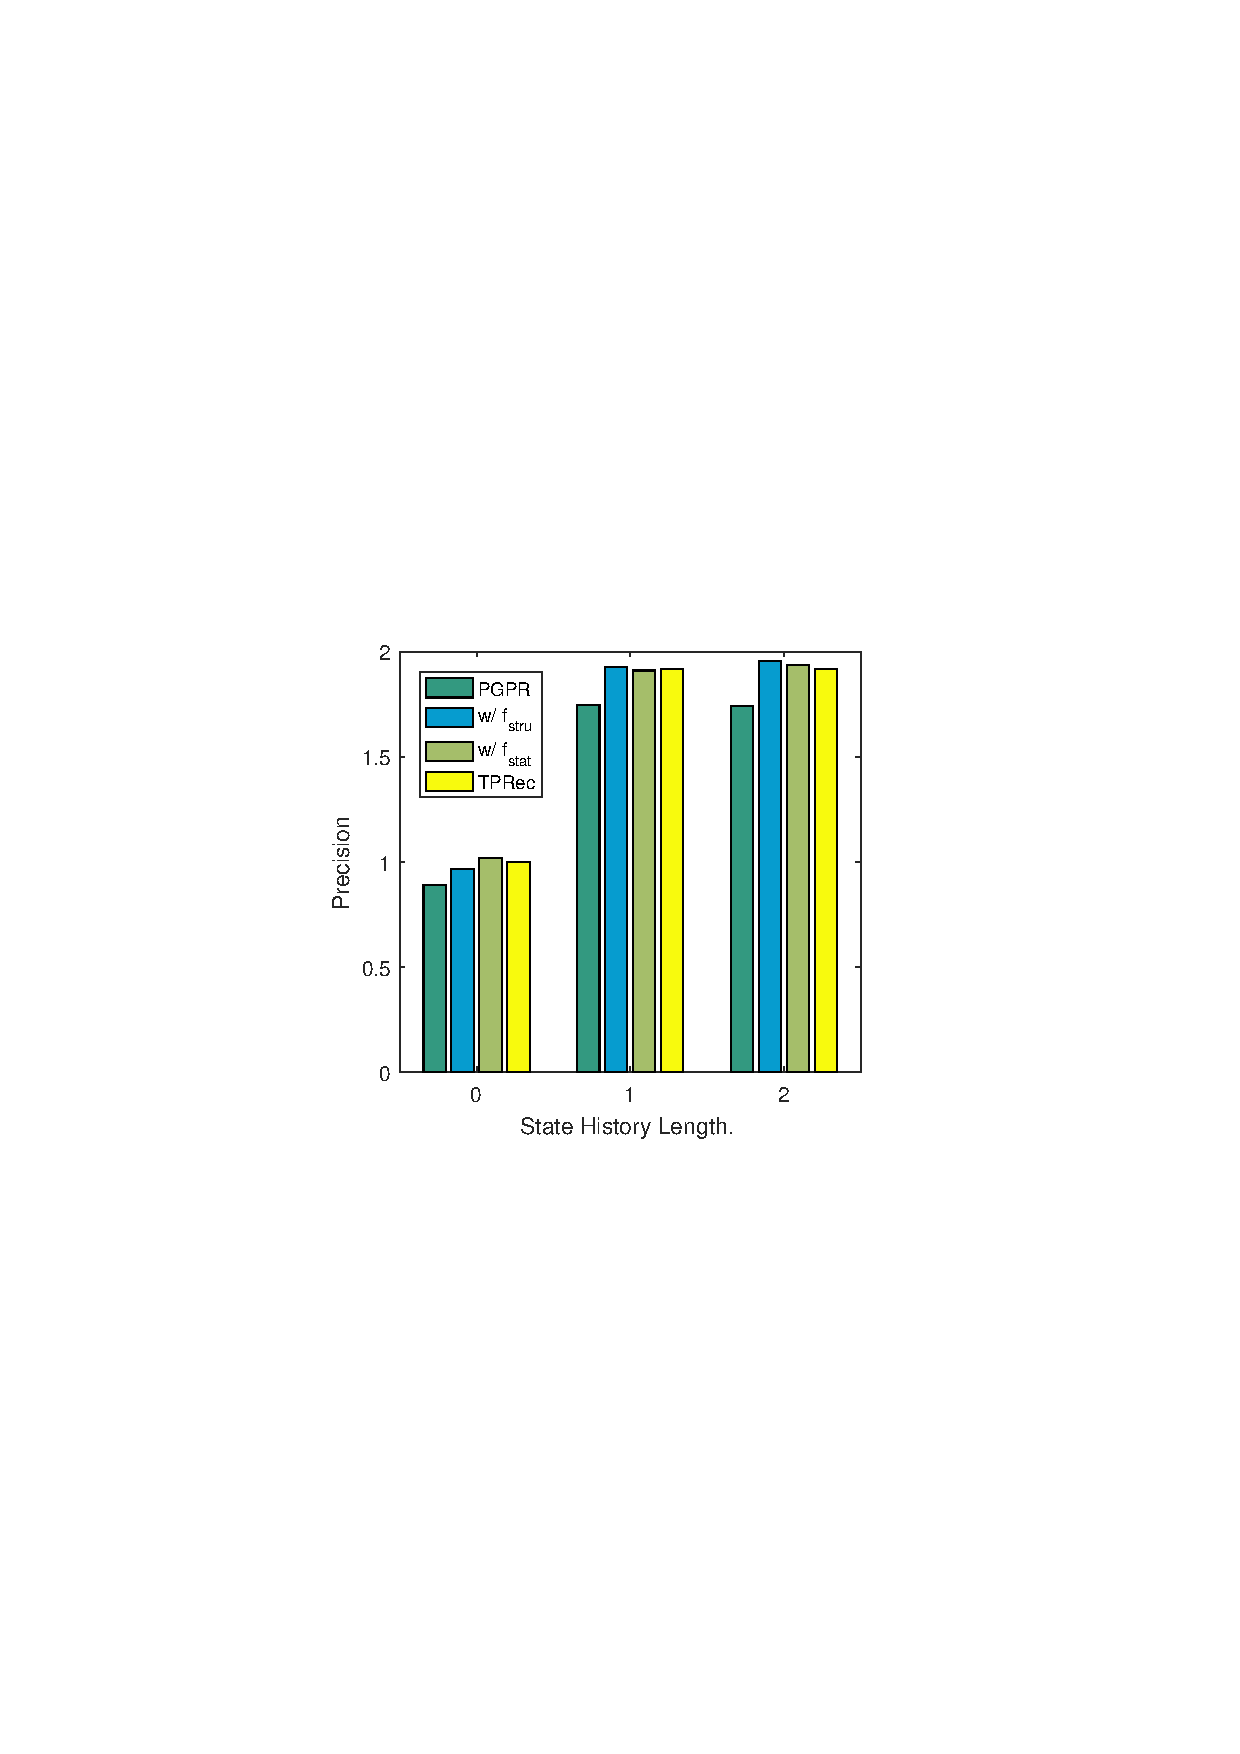
\includegraphics[width=1\textwidth]{chart/beauty_s_prec.pdf}
		\end{minipage}
	}
\caption{ Effect of varying state history length $k'$.
}
	\label{stateHistory}
\end{figure}

\subsection{Evaluating Explanations (RQ4)}
How to evaluate explanations in recommender system is a hard problem. Fortunately, inspired by \cite{countER, ADAC}, we mathematically define a user-oriented evaluation metric to evaluate explainability. And finally, we give a case study to demonstrate explanations.

\subsubsection{\textbf{Explainability Evaluation}} 
To automatically evaluate the quality of explanations generated by \tkgrec, we adopt the user's reviews on items as the ground truth reason about why the user purchased the item, as previous works\cite{countER, ADAC, chen2019co, chen2018neural, li2020generate, wang2018explainable, DIR,  wang2021towards, igv} do. Here, for reasoning paths $\tau_{u,\hat{V}}$ that an item $\hat{v} \in \hat{V}$ recommended to user $u$ before position $K$, we extract all the \textit{Word} feature entities as an explanation list, which is defined as $S_{u} = [s^{(0)}_{u}, s^{(1)}_{u}, ..., s^{(r)}_{u}]$. Thus, if a reasoning path contains more entities that are mentioned in ground truth reviews, it will achieve better explainability. More specifically, we filter less salient review words if their frequency is more than 5000 and TF-IDF < 0.1, 
and the remaining words are our ground truth reason $G_u = [g^{(0)}_{u}, g^{(1)}_{u}, ..., g^{(n)}_{u}]$.

Then for each user, we calculate the $Recall$, $Precision$ and $F_1$ score of the reasoning path's $Word$ entities $S_{u}$ with regard to the ground truth $G_u$:

\begin{align}   \label{metric_explain}
	 Recall &= \frac{|S_{u} \cap G_u|}{|G_{u}| + 1}, & Precision &= \frac{|S_{u} \cap G_u|}{|S_{u}| + 1}, &  F_1 &=  2 \cdot \frac{Precision \cdot Recall}{Precision + Recall + 1},
\end{align}
where $Recall$ measures the percentage of aspects liked by the user included in our explanation, $Precision$ indicates how much our explanation is liked by the user, and $F_1$ score is the harmonic mean between those two. And the $+ 1$ in the denominator is used to avoid dividing by $0$. Finally, we average the scores of all users to evaluate explainability. 


\begin{table}[t!]
\caption{Explanation performance comparison between PGPR and \tkgrec\ on different datasets.}\label{explainCmp}
\begin{tabular}{c|crr|crr|crr}
\hline \hline
\textbf{Dataset} & \multicolumn{3}{c|}{\textbf{Cloth}}                                                                & \multicolumn{3}{c|}{\textbf{Cellphone}}                                                            & \multicolumn{3}{c}{\textbf{Beauty}}                                                               \\ \hline
\textbf{Metric}  & \textbf{Recall}            & \multicolumn{1}{c}{\textbf{Prec.}} & \multicolumn{1}{c|}{\textbf{F1}} & \textbf{Recall}            & \multicolumn{1}{c}{\textbf{Prec.}} & \multicolumn{1}{c|}{\textbf{F1}} & \textbf{Recall}            & \multicolumn{1}{c}{\textbf{Prec.}} & \multicolumn{1}{c}{\textbf{F1}} \\ \hline
\textbf{PGPR}    & \multicolumn{1}{r}{23.771} & 90.750                             & 19.340                           & \multicolumn{1}{r}{22.970} & 90.623                             & 18.522                           & \multicolumn{1}{r}{19.296} & 90.879                             & 15.936                          \\
\textbf{\tkgrec}   & \multicolumn{1}{r}{24.642} & 90.871                             & 21.133                           & \multicolumn{1}{r}{23.637} & 90.895                             & 19.043                           & \multicolumn{1}{r}{20.093} & 90.891                    & 17.471                          \\ \hline \hline
\end{tabular}
\end{table}


From Table \ref{explainCmp}, our \tkgrec\ outperforms PGPR in all three datasets. Though not strictly, it provides an angle to show that the use of temporal information can achieve better explainability.



% From table \ref{abCmpt}, when removing personalized time-aware weighting strategy in reward, we observe significant performance degradation (higher than 69.21\%) of w/o R comparing with w/o full. w/o R even performs worse than PGPR. This interesting phenomenon clearly reveals the importance of using personalized weights. Time-aware relations are indeed useful for path reasoning, but they require to be carefully exploited. Only if we finely differentiate the contribution of each type of relation, can we sufficiently enjoy the merits of such information.

% \begin{align}   \label{metric_explain}
% 	 Precision &= \frac{|S_{u} \cap G_u|}{|S_{u}|}, & Recall &= \frac{|S_{u} \cap G_u|}{|G_{u}|}, & F_1 &=  2 \dot \frac{Precision \dot Recall}{Precision + Recall},
% \end{align}

%1. temporary加在图谱里面的情况效果用TransE本来的本知评价指标描述(introduction里面肯定
%得举个例子   -图谱为何需要时间-?);
%2. temporary用在explainable Rec里面的效果用Case study RQ1中提到的invalid users的例
%子描述.
%We model translation-based recommendation task as follows. The baseline is
%original KG
%without temporal information and encoded by TransE, and our method also
%uses TransE to encode TCKG, as mentioned in Section \ref{trl}. For a test
%couple $(User, Purchase)$,
%we generate
%corrupted products according
%to $User + Purchase \stackrel{_?}{\rightarrow} \ Product$.  Moreover, our TCKG
%embedding's
%relation $Purchase$ is adjusted to the query time from Equation \ref{rankeq}.
%We adopt the same dataset
%settings in section \ref{testdata}(70\% for training and 30\% for testing). Two
%evaluation metrics are used here, \ie, NDCG and Hit Ratio based on the top-10
%predicted items, as used in Section \ref{evalMetric}.
%As shown in Table \ref{lkCmp}, TCKG embedding performs consistently better than
%normal KG embedding, which means the temporal information we modeled does
%improve semantic information in knowledge graph and, thus, increase the recommendation results.
%
%
%The effects of using temporal information can be divided into two aspects:
%1. \textit{How does temporal information affect KG embedding?} and 2.
%\textit{How does temporal
%information benefit in explainable recommendation?} The answer to the first
%question is shown in Table \ref{lkCmp}, which compares the effects of KG
%embedding and
%TCKG embedding in translation-based recommendation\cite{transRec}. And we give
%a \textbf{case study}
%derived from
%invalid users to answer the second question.
\subsubsection{\textbf{Case Study}}
To better understand how temporal information boosts the quality of explainable recommendation, we conduct a case study based on the result of our \tkgrec. As shown in Figure \ref{caseStudy}, we provide several examples of the learned reasoning paths with hop scores, where the path marked in red denotes the top relevant one predicted by \tkgrec.
 
 
%To intuitively demonstrate the role of temporal information in
%explainable
%recommendation, we present a case study based on the results generated in the
%previous experiments. As shown in Figure \ref{caseStudy}, we extract the
%relative reasoning paths of the predicted results and red mark the higher
%ranked one.

The first example (Case 1) comes from the \textit{Clothing} dataset, where we make a recommendation for a specific user on 24-11-2013. By leveraging temporal information, our \tkgrec~ can deduce the weather is winter and correspondingly identify the most relevant word is ``cold''. Based on such knowledge, \tkgrec~ is able to retrieve more relevant ``sweater'' to the user, while PGPR that does not use temporal information would fall short. In the second example (Case 2), there are two users who both bought an ``iPhone'' on 24-3-2014 and 12-1-2014 respectively. The second user also purchased a "phone" on 05-8-2013 and a "charger line" on 11-2-2014. As we can see, our \tkgrec~ recommends ``charge line'' instead of ``phone'' as it could capture the common sense that a person is unlikely to buy two mobile phones in a short time. The last example (Case 3) depicts two reasoning paths of a user purchasing "shampoo". Our \tkgrec~ could differentiate the better one --- the red path is more reasonable, as the link ``purchase'' happened on the day 4-7-2013, which is the shopping festival as the day 11-11-2013. Naturally, the user on 11-11-2013 is more likely to have similar needs as on 4-7-2013, and the item from the red path is more likely to be favored by the user.

\begin{figure}[]
%\setlength{\abovecaptionskip}{0cm}
%\setlength{\belowcaptionskip}{0cm}
%\centerline{
\includegraphics{fig1.png}}
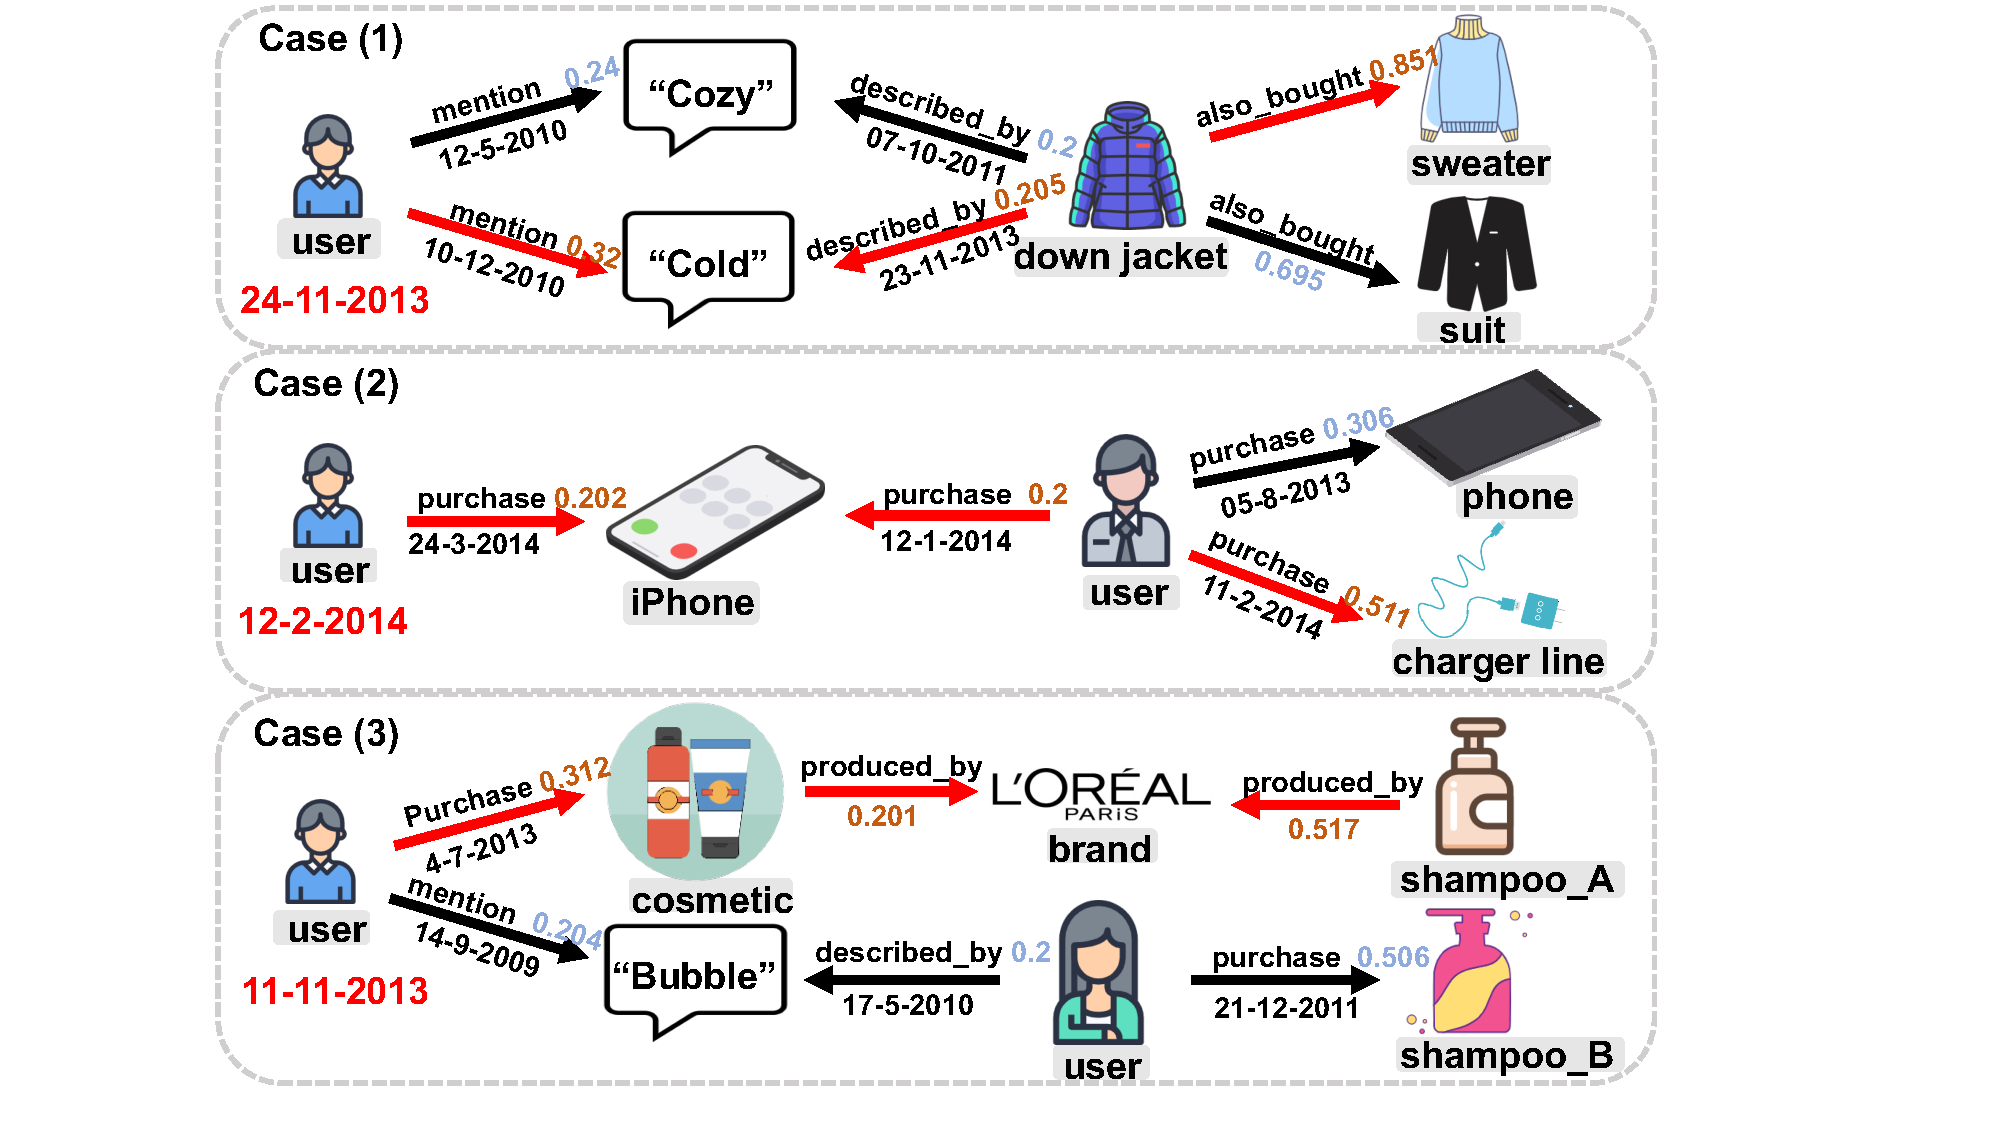
\includegraphics[width=\textwidth]{chart/caseStudy.pdf}
\caption{Case study on how temporal information benefits explainable
recommendation. The timestamp in red font below ``user'' depicts the recommended
date. The path marked in red denotes the top relevant one predicted by TPRec. }
\label{caseStudy}
\end{figure}



%needed to recommend on 24-11-2013. Since it is a winter
%recommendation, our model judged that the
%"sweater" is better than "suit", which well demonstrates the ability of our
%model to recommend in different time scenarios.
%%That means our model can capture different time scenes and give corresponding
%%recommendations.
%
%In the second example (Case 2), there are
%two "user"s both bought a "iPhone" on 24-3-2014 and 12-1-2014, and the second
%"user"
%purchased a "phone" on 05-8-2013 and a "charger line" on 11-2-2014.
%According to common sense, a person who already owns a mobile phone will hardly
%buy an old mobile phone in a short time.
%Therefore, Our model considered the "charger line" was a better choice in
%12-2-2014,
%which shows \tkgrec\ can capture the temporal dependency between hops in
%reasoning paths.
%%
%The last example (Case 3) depicts two recommended paths for user to purchase
%"shampoo". Since it is on 14-9-2009 when user mentioned "Bubble", there may
%contain the
%potential preference drift over time.
%While user purchased cosmetic on
%4-7-2013, which is shopping festival, and so is recommended time 11-11-2013.
%That means
%Our method recommended "shampoo\_A", because the path began time 4-7-2013 and
%the
%recommended time 11-11-2013 both are shopping festivals. We conclude that our
%\tkgrec\ not only achieves promising recommendation results, but also
%can efficiently find explainable reasoning paths for recommendation.


%\begin{table}[t!]
%\begin{tabular}{|c|cc|cc|cc|}
%\hline
%Methods    & \multicolumn{2}{c|}{\textbf{Clothing}}                 &
%\multicolumn{2}{c|}{\textbf{Cell Phones}}              &
%\multicolumn{2}{c|}{\textbf{Beauty}}                   \\ \hline
%Metric(\%) & \multicolumn{1}{l}{NDCG} & \multicolumn{1}{l|}{Hit Ratio.} &
%\multicolumn{1}{l}{NDCG} & \multicolumn{1}{l|}{Hit Ratio.} &
%\multicolumn{1}{l}{NDCG} & \multicolumn{1}{l|}{Hit Ratio.} \\ \hline
%Baseline   & 1.917                   & 5.482                        &
%3.472                   & 6.896                        &
%3.687                   & 10.956                       \\
%Ours.      & \textbf{2.060}          & \textbf{5.746}               &
%\textbf{3.550}          & \textbf{9.458}               &
%\textbf{3.708}          & \textbf{11.354}              \\ \hline
%\end{tabular}
%\caption{Translation-based recommendation results on three datasets between KG
%embedding and our TCKG embedding.}
%\label{lkCmp}
%\end{table}


%\subsubsection{TCKG Embedding.}
%We model translation-based recommendation task as follows. The baseline is
%original KG
%without temporal information and encoded by TransE, and our method also
%uses TransE to encode TCKG, as mentioned in Section \ref{trl}. For a test
%couple $(User, Purchase)$,
%we generate
%corrupted products according
%to $User + Purchase \stackrel{_?}{\rightarrow} \ Product$.  Moreover, our TCKG
%embedding's
%relation $Purchase$ is adjusted to the query time from Equation \ref{rankeq}.
%We adopt the same dataset
%settings in section \ref{testdata}(70\% for training and 30\% for testing). Two
%evaluation metrics are used here, \ie, NDCG and Hit Ratio based on the top-10
%predicted items, as used in Section \ref{evalMetric}.
%As shown in Table \ref{lkCmp}, TCKG embedding performs consistently better than
%normal KG embedding, which means the temporal information we modeled does
%improve semantic information in knowledge graph and, thus, increase the recommendation results.
































\section{Related Work}
\label{sec:related}

We divide the related works into three categories: (\romannumeral1) knowledge 
graph based recommendation, (\romannumeral2) temporal knowledge graph embedding
and (\romannumeral3)  temporal information in 
recommendation.


\subsection{Knowledge Graph Based Recommendation}

Existing studies on KG-based recommendation systems \cite{surveyRec} can be roughly grouped into two sub-categories: embedding-based methods and path-based
methods.

Embedding-based methods adopt a common general model, where the latent vector
$\boldsymbol{u}_i$ of each user $u_i$ and item embedding $\boldsymbol{v}_j$ can 
be
extracted from KGE, and the probability  of item $v_j$ being recommended to
user $u_i$ can be calculated by $\hat{y}_{i, j}=f\left(\mathbf{u}_{i},
\mathbf{v}_{j}\right)$. Note that $f(\cdot)$ can be either DNN, inner product,
or other scoring functions.  
%
For instance, \cite{CKE} proposed CKE, which uses TransE to unify the KG information in the CF framework.
%
Deep Knowledge-based Network (DKN) \cite{DKN} treats entity embeddings and word embeddings as different channels, where Kim CNN \cite{kimCNN} is used to combine them together for news recommendation.
\cite{KSR} uses a GRU network with a knowledge-enhanced key-value memory network, named KSR, to capture user preferences from the sequential interactions.
\cite{kgat} and \cite{kgin} employ the message passing mechanism of graph neural networks over KG to model the higher-order connections among users, entities, and items.


In the line of path-based methods, recommendations are made based on the connectivity patterns of the entity in user-item graph.
For example, \cite{mcrec} uses CNN to obtain each path instance's embedding.
%
\cite{kprn} proposed a knowledge-aware path recurrent network (KPRN) solution,
which constructs the extracted path sequence with both the entity embedding and
the relation embedding, and encodes the path sequence with an LSTM layer before
recommendation.  
%
RippleNet~\cite{ripplenet} combined embedding-based and path-based methods and
modeled users' preference propagation by their historical interests along the
path in the KG. 
%
Inspired by KG reasoning techniques~\cite{deeppath, multihop, gowalk}, PGPR~\cite{pgpr} performs reinforcement policy-guided path reasoning over
KG-based user-item interaction.
Inspired by such RL-based policy networks, CPR~\cite{RLconversa} models conversational recommendation as a path reasoning problem on a heterogeneous graph.
Different from PGPR which relies on sparse reward signal, ADAC~\cite{ADAC} adopts an Adversarial Actor-Critic model to achieve faster converge. 

These KG reasoning methods (\eg,~\cite{pgpr, ADAC, RLconversa}) can provide explainable reasoning paths while obtaining accurate recommendation results.
However, they do not use temporal information and may lead to inappropriate
recommendations.
Therefore, we propose \tkgrec, aiming to leverage temporal information for promoting explainable recommendation.


%\subsection{Squential Recommendation}
%Sequential recommendation captures patterns between consecutive user-item 
%interactions and predicts the successive item that the user is likely to 
%adopt. 
%A classic work is the FPMC model \cite{rendle2010fFPMC}, which integrates
%matrix factorization with Markov chains for modeling long-term perferences and 
%dynamic transitions of users.

\subsection{Temporal Knowledge Graph Embedding}


Existing studies on knowledge graph embedding research focus on static
knowledge graphs. A series of these models are variations of 
TransE~\cite{transE, transD,
transH, transR}. These models assume that facts are not changing with time, which is
obviously contrary to reality. 
%
Therefore, recent studies begin to take temporal information (\eg , fact
occurrence time, end time, \etc)
%
%\footnote{\hxie{what do you mean by ``fact \textit{occursSince} when \etc''}}
%
into consideration \cite{surveyKG}, which turns out to further improve the
performance of KG embedding.

There exist only a few studies on temporal knowledge graph (TKG) embedding. 
%
\cite{leblay} proposed TTransE by simply extending existing
embedding methods like TransE. TTransE adopts translational distance score
functions to learn associations between facts of a KG.
%and encode time information in entity-relation to low dimensional spaces. 
%
\cite{ma_embedding} generalized existing models for static
knowledge graphs to temporal knowledge graphs with a timestamp embedding. 
%
\cite{hyte} took a timestamp as a hyper-plane and projected
entities and relations to learn KG embedding. 

TKG embedding has to deal with two types of dynamics, namely,
entity dynamics and relation dynamics.

Entity dynamics refers to the fact that real-world events can
change the state of a given entity's state and therefore affect its
corresponding relations. 
%
\cite{knowevolve} modeled the occurrence of a fact as a
temporal point process, and used a novel recurrent network to learn the
representation of non-linearly evolving entities. 
%
\cite{contextTemporal} formulated the temporal scoping
problem as a state change detection problem and utilized the context to learn
the states and the state change vectors.

Relation dynamics refers to the fact that the relations
among entities in a knowledge graph may change over time. 
%
\cite{relation_dy} realized that there exist temporal
dependencies in relational chains following the timeline, for example,
$(P,\text{wasBornIn}, \_ )$ $ \rightarrow$ $ (P, $ $ \text{graduateFrom}$ $, $ $\_ ) $ $\rightarrow $ $(P, \text{workAt}, \_ ) $
$\rightarrow $ $(P,\text{diedIn}, \_ )$, and found that many facts are only
valid during a short time period. To solve that issue, the authors proposed two
time-aware KG completion models to incorporate the above two kinds of temporal
information.

%Numerous experiments demonstrate effectiveness of those TKG embedding methods
%over traditional KG embedding methods in different tasks, which illustrates
%the auxiliary role of temporal information in representation.
%%%%%%%%%%%%%%%%%%%%%%%%%%%%%%%%%%%%%%%%%%%%%%%%%%%%%%%%%%%%%%%%%%%%%%%%%%%%%%%%%
Although those TKG embedding methods achieve better
performance than traditional KG embedding methods, 
none of them have considered if only part of the facts is updated very frequently, which is common in recommendation
and dealed by our \tkgrec.
%%%%%%%%%%%%%%%%%%%%%%%%%%%%%%%%%%%%%%%%%%%%%%%%%%%%%%%%%%%%%%%%%%%%%%%%%%%%%%%%%

\subsection{Temporal Information in Recommendation}

Temporal Information is important contextual information for providing users 
with an accurate prediction based on historical behaviors\cite{timeSurveyReview}.
\cite{yi2014beyond} finds that dwell time is an important factor to quantify how likely an item is relevant to a user.
\cite{liang2012time} uses the temporal information in micro-blogs in order to profile users' time-sensitive topic interests.
\cite{chang2017streaming} proposes sREC, which captures temporal dynamics of users and topics under steaming settings, to perform real-time recommendations.
\cite{seqInMusic} proposes CoSeRNN and leverages time context and device context for better music recommendation.
As for temporal patterns of user behaviors, \cite{timeMatters} and \cite{timeAwareSeq} discover ``absolute" and ``relative" time patterns and jointly learn those temporal patterns to model user dynamic preferences and predict future items.
\cite{heteTemporal} defines the periodic and evolving patterns of user preferences, and proposes a cascade of two encoders with an attention module to capture such temporal patterns.

Recently, KG-based methods achieve great success for many temporal tasks.
\cite{kerl} uses both sequence- and knowledge-level state representations to capture user preference with an induction network, and adopt a composite reward to capture both sequence-level and knowledge-level information for sequential recommendation.
\cite{KSR} uses GRU to capture the user’s sequential preference, and utilizes knowledge base information to model the user’s attribute-level preference.
\cite{huang2019explainable} designs EIUM, which represents KG with 
multi-modal fusion, and adopts a masked self-attention model to encode the user’s sequential interactions for capturing her dynamic interests.
Most of those methods with temporal information consider KG information as enhanced representation to assist sequential recommendation.
Our work differs from these works by modeling the statistical and structural 
temporal patterns between user-item interactions to construct TCKG, and propose time-aware path reasoning over the TCKG to make full use of the structural constraints in KG. It's inconvenient to utilize our \tkgrec\ to predict the next item task like other sequential recommendation methods, because the KG data is different from the sequence data. That is, we need to construct a dynamic edge MASK matrix on KG's adjacency matrix to avoid the next item $v$'s information and other items behind $v$ from influencing the training phase. We will leave this as our future work.
% If we superimpose T to predict the next item,
%Sequential recommendation captures patterns between consecutive user-item 
%interactions and predicts the successive item that the user is likely to 
%adopt. 
%A classic work is the FPMC model \cite{rendle2010fFPMC}, which integrates
%matrix factorization with Markov chains for modeling long-term perferences and 
%dynamic transitions of users.
% (5) Thank you for pointing out such interesting direction. The motivation of our reward function is mentioned in ans.(2). We haven't considered to take the user's recently interacted items v as the pre-known target items, and set the reward function as the similarity between the reasoning terminal item $\hat{v}$ and $v$. However, the KG data is different with sequence data. That is, we need to construct a dynamic edge MASK matrix on KG's adjacency matrix to avoid items $v$'s information and the other items behind v from influencing the training phase. We will leave this as our future work. \\


















\section{Conclusion}
\label{sec:conclusion}

In this paper, we present \tkgrec, a novel 
time-aware path reasoning model for recommendation, which addresses the timeliness of
interpretation.
To the best of our knowledge, the \tkgrec\ method is the first work to
introduce time-aware path reasoning method into a recommendation
system and achieves significant performance improvement by leveraging the
temporal information.
%
%To the best of our knowledge, the \tkgrec\ method is the first work to
%introduce time-aware reasoning method into a recommendation
%system and achieves significant performance improvement by leveraging the
%temporal information.
%
%Our model consists of time-aware interaction relation extraction component, which 

Our model first uses time-aware interaction relation extraction component to
construct TCKGs for the
reasoning environment. Then the time-aware representation learning component encodes 
entities and relations to get proper
representation. Finally is the key time-aware reasoning component, which adopts a 
time-aware
personalized reasoner to explore temporal information assisted recommendation.
%
We also conduct extensive experiments on three real-world datasets to evaluate
the effectiveness of \tkgrec. Evaluation results demonstrate that \tkgrec\
outperforms the existing models on a set of widely used metrics.

For future work, we plan to evaluate \tkgrec\ using more datasets from other
product domains and other major online vendors, transform the training process 
to make it suitable for next item prediction,
% Change the training process to make it suitable for sequence recommendation
and extend our \tkgrec\ model
by leveraging the adversarial learning model to automatically shape rewards in
order to achieve more accurate recommendation results.  We also plan to combine
causal inferences with our model to achieve better interpretability.


\section{ACKNOWLEDGMENTS}
This work is supported in part by National Key R\&D Program of China (Grant No. SQ2021YFC3300088), the National Natural Science Foundation
of China (Grant 62102382, U19A2079, No. U19B2036),  USTC Research
Funds of the Double First-Class Initiative (WK2100000019), and the National Key R\&D Program of China (2021ZD011802).

%%
%% Keywords. The author(s) should pick words that accurately describe
%% the work being presented. Separate the keywords with commas.


%%
%% The next two lines define the bibliography style to be used, and
%% the bibliography file.
\bibliographystyle{ACM-Reference-Format}
\bibliography{sigproc}


\end{document}
\endinput
%%
%% End of file `sample-acmsmall.tex'.
